\chapter{Keyword Reference}
\label{chap:keyword-reference}

This chapter documents the unified FEMaster input language:
supported Abaqus-compatible definitions, CalculiX-compatible aliases,
and FEMaster-specific extensions can be used together. Keywords are
organized by modelling role. Section~\ref{sec:keyword-index}
provides a compact index.

\paragraph*{Reading the keyword pages}

Each keyword has one canonical entry, beginning with its modelling
purpose and supported parameters or data lines. An example of that
keyword follows. Where a genuinely useful alternative exists, it is
shown directly below the primary example. Abaqus compatibility and
FEMaster extensions are identified without presenting separate input
languages. The \cmd{ELEMENT} reference additionally documents the
individual numerical formulations and their accepted type aliases.

\section{Input Structure}
\label{sec:input-format}

FEMaster reads a unified keyword-based input language. A command
begins with an asterisk, optional parameters follow after commas,
and keyword-specific data are provided on subsequent lines.
Supported Abaqus and CalculiX input forms coexist with FEMaster
extensions in the same deck; selecting a particular file format
or parser is not required.

Familiar Parts, Assemblies, Steps, loads, and boundary conditions
can therefore be combined with FEMaster features such as named
load and support collectors, explicit LOADCASE definitions,
generic Fields, and solver controls. Each keyword page presents
a preferred example and, where meaningful, additional supported
alternatives below it rather than in parallel columns.

\subsection{Command lines}

A command line begins with \texttt{*}. The command name follows immediately and may be followed by comma-separated parameters. Parameters can be key/value pairs or flags. Data lines continue until the next command line begins.

\begin{syntax}
*COMMAND, KEY=value, FLAG
value, value, value
value, value, value
\end{syntax}

Command and parameter names are case insensitive. Whitespace inside command names is ignored, so compact names such as \cmd{SOLIDSECTION} and spaced names such as \cmd{SOLID SECTION} refer to the same command where that keyword is supported. The manual normally uses the spaced form when it improves readability and the compact form where it is customary in native FEMaster decks.

Parameter values retain their meaning. Numerical values are read as integer or floating-point quantities according to the keyword definition. Boolean-style options may appear as flags or as explicit values where documented. Names are used to reference Parts, Instances, sets, surfaces, materials, sections, coordinate systems, Fields, amplitudes, collectors, and other model entities.

\subsection{Data lines and multiline records}

The number and meaning of data-line entries depend on the keyword. Some commands accept one record per line, such as \cmd{NODE}. Others read a fixed-size group of values, a matrix, a list of identifiers, or multiple records. The keyword pages describe the required ordering explicitly.

Comma-separated values preserve the visibility of optional empty entries. Whitespace around values is ignored. Several native FEMaster commands use the literal \val{NAN} to mean that a generalized component is not prescribed. This is different from zero: zero is a physical numerical value, whereas an empty or NaN component may mean ``leave this degree of freedom unspecified'' for the corresponding keyword.

Long connectivity or data records may continue over more than one physical line where that command permits multiline input. This representation accommodates higher-order elements and large fixed-size material or Section definitions.

\subsection{Scopes}

Several keywords open scopes. A Part contains reusable mesh topology and part-level regions. An Assembly contains Instance placement and assembly-level region definitions. Material subcommands apply to the active material. Native FEMaster \cmd{LOADCASE} opens an analysis definition. Abaqus \cmd{STEP} opens an Abaqus analysis step.

Scopes are defined by keywords, not by indentation. Indentation may be used for readability but has no syntactic meaning. Closing commands such as \cmd{END PART}, \cmd{END ASSEMBLY}, \cmd{END INSTANCE}, \cmd{END STEP}, and native \cmd{END} make the end of the corresponding scope explicit.

Parts, Assemblies, and Instances are optional for simple native FEMaster models. Nodes and elements may be defined directly without constructing an explicit Assembly. The structured form represents reusable Parts, repeated Instances, independent local ID spaces, and assembly-level selections.

\paragraph{Optional native \cmd{MODEL} marker.}
Native FEMaster may optionally place \cmd{MODEL} at root level as a descriptive marker. It does not open a scope, create a second model object, or select among several models; omitting it has no effect on the topology or analysis. \key{NAME} is optional and may be used to attach a descriptive model name.

\begin{syntax}
*MODEL, NAME=BRACKET_MODEL
\end{syntax}

This marker is part of the native input-file framing rather than a separate model-definition hierarchy level. Abaqus input does not require or use a corresponding wrapper.

\subsection{Names, identifiers, and references}

Node and element IDs are user-defined non-negative integer labels. They may start at \textbf{0}; they do not need to start at 1 and do not need to be contiguous. IDs only need to be unique within the topology scope in which they are defined. For example, \val{0}, \val{10}, and \val{1000} are valid node IDs.

Inside separate Parts, the same numerical ID may be reused because each Part has its own local topology. Instances preserve these local labels from the user's point of view. When an assembly-level command needs to identify an entity from a particular Instance, the documented Instance-qualified reference syntax is used.

Named resources are used throughout the rest of the deck. Node sets, element sets, surfaces, materials, profiles, orientations, Fields, amplitudes, collectors, and other definitions are referenced by name. Stable names expose the model structure without repeatedly addressing individual numerical IDs.

\emph{User IDs} and \emph{local positional indices} represent different concepts. User node and element IDs may be sparse and may include zero. By contrast, indices such as a Field's \val{local_node}, \val{local_ip}, or \val{local_mp} identify a position inside an element and are explicitly zero based where documented.

\subsection{FEMaster and Abaqus examples in this manual}

Each keyword page shows a primary definition with useful alternatives
stacked directly below it. A given keyword may have Abaqus-compatible
or FEMaster-specific data forms; their placement and limitations are
defined by that keyword rather than by separate input dialects.
For example, \cmd{SOLVER} belongs inside a \cmd{LOADCASE} or inside
a \cmd{STEP} after its procedure definition.

The comparison shows how the same model operation is expressed in either accepted input style without exposing parser implementation details.

\keywordpage{HEADING}

\cmd{HEADING} adds descriptive text to an input deck. It does not change the finite-element equations or the numerical result. The keyword keeps exported, archived, and regression decks self-describing and is accepted in both native FEMaster and Abaqus input.

A heading is metadata conventionally placed near the beginning of a file. Later model commands do not reference it by name, and it does not substitute for a Part name, material name, loadcase name, or other actual model identifier.

Native FEMaster also accepts the optional root-level \cmd{MODEL, NAME=...} marker described above. \cmd{HEADING} is free descriptive text, whereas \cmd{MODEL} is a compact native file marker.

\syntaxheading

\begin{syntax}
*HEADING
Descriptive model title
\end{syntax}

\exampleheading

\begin{inputdeck}[Abaqus-compatible]
*HEADING
Cantilever verification model
\end{inputdeck}


\section{Model Definition}
\label{sec:model-definition}
A FEMaster model can be defined directly through nodes and elements
or organized into reusable Parts and placed Instances. The optional
Part/Assembly hierarchy supports multiple placements of the same
component with independent local numbering; simple models can omit
the hierarchy. Node and element IDs are non-negative user labels,
including \val{0}, and need not be consecutive.

Named node sets, element sets, and surfaces provide reusable selections
for Section assignments, loads, supports, and constraints. The
following keywords define the mesh, its organization, and its
associated regions.

\keywordpage{PART}

\cmd{PART} begins a reusable finite-element component definition. Nodes, elements, part-level sets, surfaces, and section assignments that follow belong to the active Part until \cmd{END PART} closes it.

A Part is defined in its own local coordinate system. Its node coordinates describe the undeformed component geometry before any Instance placement. The Part itself has no global translation or rotation. If the same component is needed in several locations, define its topology once and create several \cmd{INSTANCE} entries.

Part-local IDs are independent. Node \val{0} in Part \val{LEFT} and node \val{0} in Part \val{RIGHT} are different nodes even though they use the same numerical label. The same applies to element IDs. This is one of the main practical advantages of the Part representation: imported or reusable components do not need to be renumbered merely because another Part uses the same IDs.

Explicit Parts are optional in native FEMaster input. If nodes and elements are written directly at root level, they belong to the flat model topology and can be used without writing \cmd{PART}, \cmd{ASSEMBLY}, or \cmd{INSTANCE}.

Part-level sets, surfaces, and Section assignments follow the Part when it is instantiated. Part-level definitions therefore describe properties intrinsic to every placed copy, whereas Assembly-level definitions can select or combine particular Instances.

\begin{keywordparameters}
\key{NAME} & required & Unique Part name. The name is referenced by \cmd{INSTANCE}. \\
\end{keywordparameters}

\exampleheading

\begin{inputdeck}
*PART, NAME=ROD
*NODE, NSET=PNODES
0,   0., 0., 0.
1, 100., 0., 0.
*ELEMENT, TYPE=T3D2, ELSET=BAR
0, 0, 1
*END PART
\end{inputdeck}


\keywordpage{END PART}

\cmd{END PART} closes the active Part scope. Definitions that follow are no longer part-local unless another \cmd{PART} is opened. The command is distinct from native \cmd{END}, which terminates a native loadcase.

\syntaxheading

\begin{syntax}
*END PART
\end{syntax}

\exampleheading

\begin{inputdeck}
*PART, NAME=PLATE
...
*END PART
\end{inputdeck}

\keywordpage{ASSEMBLY}

\cmd{ASSEMBLY} begins the optional Assembly scope. The Assembly is where placed Instances and regions that refer to the assembled model are defined. A model that does not need explicit Instances may omit this scope entirely.

The Assembly combines several Parts or repeated placements of one Part. Part-level topology remains expressed with local IDs, while Assembly-level sets and surfaces select entities from particular Instances. This preserves local numbering inside each component without forcing a single manually renumbered global mesh.

The Assembly organizes the placed model but is not required by the solver. A flat native model and a structured Assembly represent alternative organizational forms for the same finite-element topology.

\key{NAME} is optional and defaults to \val{ASSEMBLY}. The name is descriptive for the supported current workflow; Instances and assembly-level regions are the referenced objects inside the Assembly.

\begin{keywordparameters}
\key{NAME} & optional & Assembly name; default \val{ASSEMBLY}. \\
\end{keywordparameters}

\exampleheading

\begin{inputdeck}
*ASSEMBLY, NAME=ASSEMBLY
*INSTANCE, NAME=ROD_A, PART=ROD
0., 0., 0.
*END INSTANCE
*END ASSEMBLY
\end{inputdeck}

\keywordpage{END ASSEMBLY}

\cmd{END ASSEMBLY} closes the Assembly scope.

\syntaxheading

\begin{syntax}
*END ASSEMBLY
\end{syntax}

\exampleheading

\begin{inputdeck}
*ASSEMBLY, NAME=ASSEMBLY
*INSTANCE, NAME=LEFT, PART=ROD
0., 0., 0.
*END INSTANCE
*END ASSEMBLY
\end{inputdeck}


\keywordpage{INSTANCE}

\cmd{INSTANCE} places an existing Part in the Assembly. Native FEMaster intentionally accepts the same placement representation used by the supported Abaqus reader. \key{NAME} gives the Instance a unique assembly name and \key{PART} selects the reusable Part.

An Instance may be placed by translation, rotation, both, or neither. A three-value data line gives a translation
\[
\boldsymbol t=(t_x,t_y,t_z).
\]
A seven-value line defines a rotation by two points on the rotation axis and an angle in degrees:
\[
(x_1,y_1,z_1,x_2,y_2,z_2,\varphi).
\]
The two axis points must be distinct. If both translation and rotation are supplied, the translation is applied first and the axis-angle rotation second. With no placement data the Part is instantiated in its original position.

Instance placement changes the position and orientation of the component in the assembled model; it does not require the Part coordinates or Part IDs to be rewritten. Several Instances may therefore reference the same Part with different placements.

The Part-local node and element labels remain associated with every Instance. Assembly-level sets use the Instance qualification to distinguish the same local ID in several placed copies.

\begin{keywordparameters}
\key{NAME} & required & Unique Instance name used for assembly-level references. \\
\key{PART} & required & Name of the Part to place. \\
\end{keywordparameters}

\begin{keyworddata}
\val{tx, ty, tz} & Optional translation vector. \\
\val{x1,y1,z1,x2,y2,z2,angle} & Optional rotation axis through two points and rotation angle in degrees. \\
\end{keyworddata}

\exampleheading

\begin{inputdeck}
*INSTANCE, NAME=RIGHT, PART=BRACKET
100., 0., 0.
0., 0., 0., 0., 0., 1., 90.
*END INSTANCE
\end{inputdeck}

\keywordpage{END INSTANCE}

\cmd{END INSTANCE} closes the current Instance definition.

\exampleheading

\begin{inputdeck}
*INSTANCE, NAME=A, PART=BLOCK
20., 0., 0.
*END INSTANCE
\end{inputdeck}

\keywordpage{NODE}

\cmd{NODE} defines finite-element nodes by user ID and Cartesian reference coordinates. In a Part scope the nodes belong to that Part. In a flat native model they belong directly to the model topology.

Node IDs are non-negative integers. \textbf{ID 0 is valid.} IDs need not be contiguous and may be chosen to preserve meaningful numbering from a mesh generator or external model. They must only be unique within the topology scope in which they are defined.

The optional \key{NSET} parameter adds every node in the block to a node set. Native FEMaster defaults this set to \val{NALL}. Coordinates are Cartesian reference coordinates. Missing trailing coordinate components default to zero; explicit three-component coordinates expose the complete position in shared examples.

Node order has no mechanical meaning by itself, but the order in which node IDs appear in an element connectivity is crucial because it determines the element's local topology and orientation.

The coordinates define the undeformed geometry. Loads, prescribed displacements, initial velocities, and Instance placement do not change the meaning of the node's Part-local reference coordinates.

\begin{keywordparameters}
\key{NSET} & optional & Node set receiving all nodes in the block; native default \val{NALL}. \\
\end{keywordparameters}

\begin{keyworddata}
\val{id} & Non-negative user node ID; \val{0} is valid. \\
\val{x, y, z} & Cartesian reference coordinates. \\
\end{keyworddata}

\exampleheading

\begin{inputdeck}
*NODE, NSET=EDGE
0,  0., 0., 0.
10, 25., 0., 0.
20, 50., 0., 0.
\end{inputdeck}

\keywordpage{ELEMENT}

\cmd{ELEMENT} defines element topology and connectivity. Each data
record starts with an element ID followed by the node IDs in
formulation-specific order. The \key{TYPE} parameter selects the
formulation, while \key{ELSET} optionally assigns the elements to a
named set. Element IDs are non-negative user labels, may start at
\val{0}, and need not be consecutive.

Connectivity order matters: it defines local edges and faces,
element orientation, shell normals, and the mapping between the
reference element and its physical geometry. The connected nodes
must belong to the same topology scope as the element.

\begin{syntax}
*ELEMENT, TYPE=<element-type>, ELSET=<set>
<element-id>, <node-1>, <node-2>, ...
\end{syntax}

\begin{keywordparameters}
\key{TYPE} & required & Element type or formulation identifier listed below. \\
\key{ELSET} & optional & Element set receiving the block; the general set \val{EALL} is used by default. \\
\end{keywordparameters}

\begin{keyworddata}
\val{id} & Non-negative element ID; \val{0} is valid. \\
\val{n1, n2, ...} & Node connectivity in formulation-specific order. \\
\end{keyworddata}

Element connectivity defines topology and kinematics, but additional
physical properties are assigned by the applicable Section or
concentrated-property keywords; see Section~\ref{sec:sections}.
The following element reference lists the supported types and their
aliases, followed by the individual numerical formulations, connectivity,
applications, and limitations.

% Included directly inside the *ELEMENT keyword entry.
% Families are subsubsections; individual formulations are paragraphs.
\addtocontents{toc}{\protect\setcounter{tocdepth}{4}}

The selected element type determines kinematics, interpolation,
integration scheme, and recoverable mechanical quantities. The overview
groups alternative input names of the same implementation; the detailed
descriptions cover connectivity, applications, and limitations.

\subsubsection{Supported element types}
\label{sec:elements}

Each row describes one implemented formulation. Alternative accepted
\key{TYPE} names are grouped in the same row; they select the same
FEMaster implementation rather than distinct numerical elements.

\begin{longtable}{@{}p{0.33\linewidth}p{0.09\linewidth}p{0.49\linewidth}@{}}
\toprule
\textbf{Element type and aliases} & \textbf{Nodes} & \textbf{Formulation} \\
\midrule
\endhead
\val{C3D4} & 4 & Linear tetrahedral solid. \\
\val{C3D5} & 5 & Five-node pyramid represented by a degenerated hexahedral topology. \\
\val{C3D6} & 6 & Linear wedge solid. \\
\val{C3D8} & 8 & Fully integrated linear hexahedral solid. \\
\val{C3D8I} & 8 & Incompatible-mode hexahedral solid with condensed enhanced modes. \\
\val{C3D8R} & 8 & Reduced-integration hexahedral solid with hourglass stabilization. \\
\val{C3D10} & 10 & Quadratic tetrahedral solid. \\
\val{C3D13} & 13 & Quadratic pyramid solid with rational interpolation. \\
\val{C3D15} & 15 & Quadratic wedge solid. \\
\val{C3D20} & 20 & Fully integrated quadratic hexahedral solid. \\
\val{C3D20R} & 20 & Reduced-integration quadratic hexahedral solid. \\
\val{MITC3FRT}, \val{S3}, \val{S3R} & 3 & Finite-rotation triangular shell. \\
\val{MITC4FRT}, \val{S4}, \val{S4R}, \val{MITC4} & 4 & Finite-rotation quadrilateral MITC shell. \\
\val{MITC6FRT}, \val{S6}, \val{S6R} & 6 & Quadratic finite-rotation triangular shell. \\
\val{MITC8FRT}, \val{S8}, \val{S8R}, \val{MITC8} & 8 & Quadratic finite-rotation quadrilateral MITC shell. \\
\val{B31} & 2 & Shear-flexible geometrically exact three-dimensional beam. \\
\val{B33} & 2 & Three-dimensional Euler--Bernoulli beam. \\
\val{T3}, \val{T3D2} & 2 & Three-dimensional axial truss. \\
\val{MASS} & 1 & Concentrated translational mass. \\
\val{ROTARYI} & 1 & Concentrated rotary inertia. \\
\val{SPRING1} & 1 & Point-to-ground spring in a generalized nodal direction. \\
\val{QSPT} & 4 & Specialized quadrilateral shear-panel element. \\
\bottomrule
\end{longtable}

The table describes accepted input names, not numerical equivalence
with the corresponding elements in other finite-element solvers.
In particular, the \val{R} suffix of imported shell names such as
\val{S4R} does not select a separate reduced-integration
formulation in FEMaster.

\clearpage
\subsubsection{Solid elements}

Solid elements model a three-dimensional continuum. They use translational nodal degrees of freedom and obtain their constitutive response from a \cmd{SOLID SECTION}. They represent the full three-dimensional stress state, through-thickness stresses, and local geometry or load introduction that shell and line elements omit.

Low-order solids are inexpensive but may require significant refinement in bending-dominated problems. Higher-order solids generally represent curvature and stress gradients more efficiently, but they contain more degrees of freedom per element and are more sensitive to poor midside-node placement and distorted mappings. Well-shaped hexahedra are useful for structured or swept meshes, while tetrahedra and pyramids accommodate irregular geometry and mixed-topology transitions. Reduced integration introduces additional sensitivity to low-energy modes and stabilization. Mesh quality and refinement should be assessed using displacements, reactions, energies, and stress trends; convergence of the algebraic solver alone does not establish discretization accuracy.

\clearpage
\paragraph{\val{C3D4}: 4-node tetrahedral solid}

\begin{figure}[H]
    \centering
    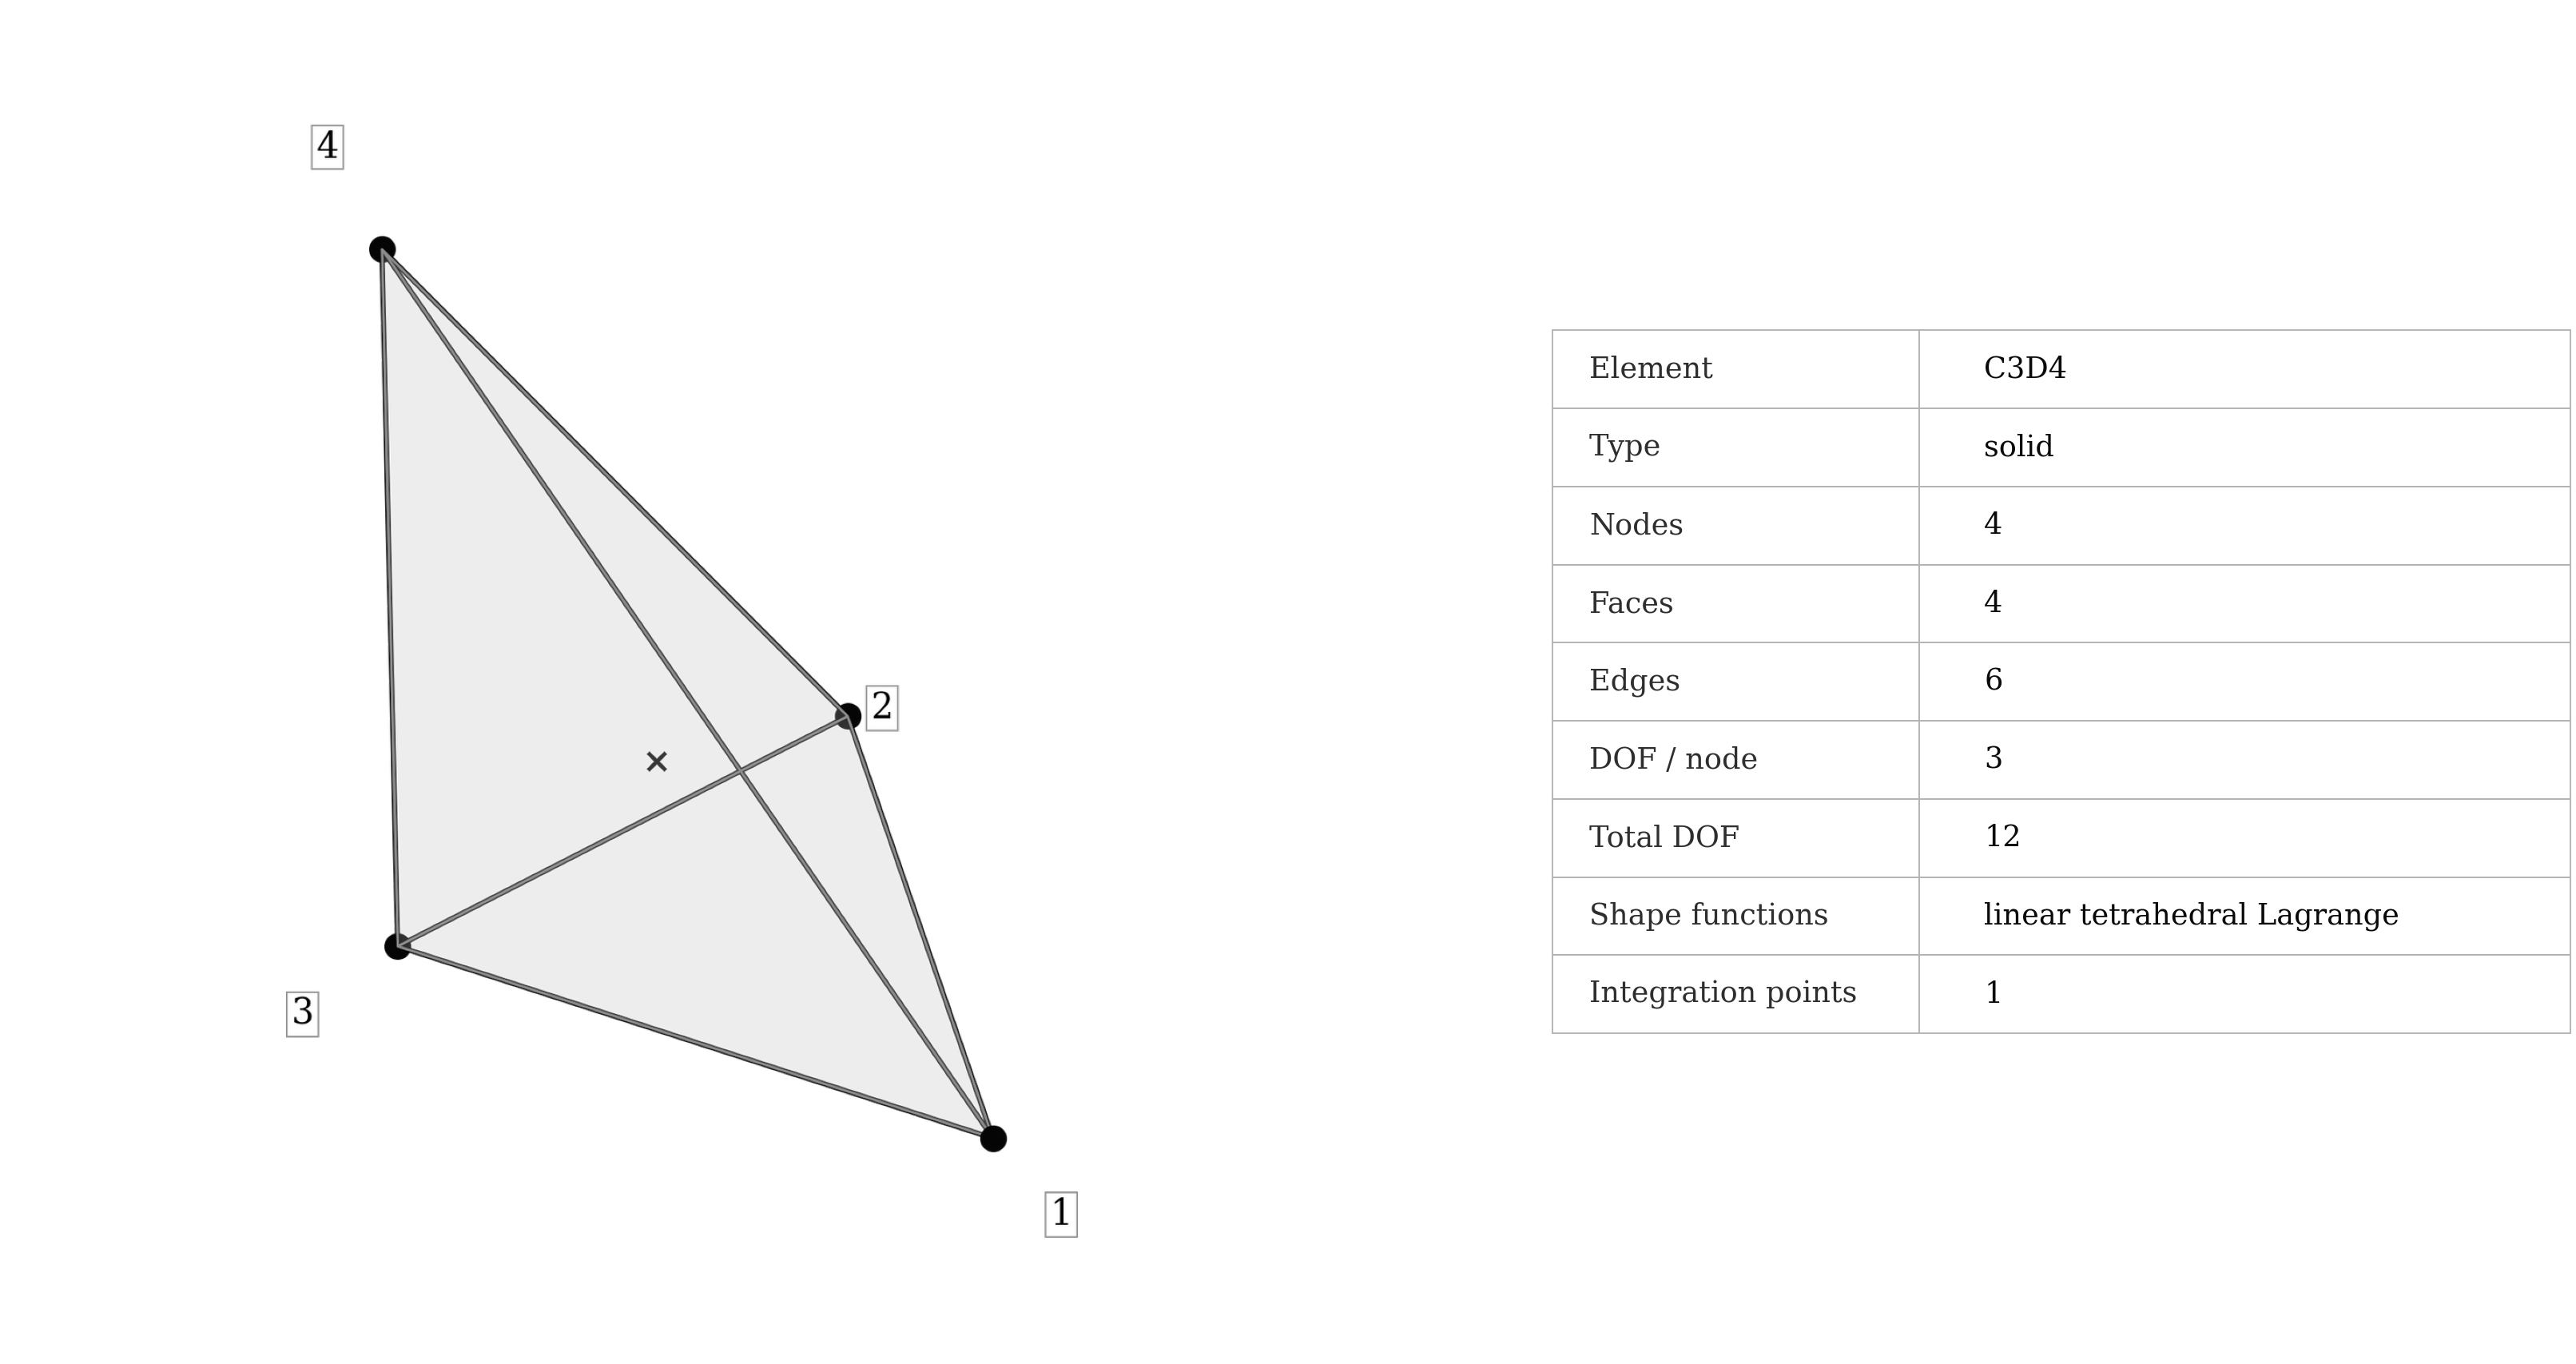
\includegraphics[width=0.78\linewidth]{pages/figures/element_schematics/c3d4_schematic.png}
    \caption{\val{C3D4} element topology and integration scheme.}
\end{figure}

\begin{syntax}
*ELEMENT, TYPE=C3D4, ELSET=<set>
<id>, <n1>, <n2>, <n3>, <n4>
\end{syntax}

\val{C3D4} is the simplest three-dimensional continuum element in FEMaster. It uses four corner nodes and linear displacement interpolation over a tetrahedral reference domain. The resulting strain field is constant within one element, which makes the element inexpensive and geometrically easy to mesh but limits the deformation and stress gradients that a single element can reproduce.

The principal advantage of \val{C3D4} is meshing flexibility. Tetrahedra can fill complex CAD volumes, narrow transitions, and irregular local details with little manual topology design. This supports early stiffness checks, coarse load-path studies, and robust automatic meshing at the cost of stress accuracy per degree of freedom.

The limitation is stiffness and stress resolution. Linear tetrahedra tend to be overly stiff in bending-dominated problems unless the mesh is fine. Since the strain state is constant in each element, stress fields can appear piecewise constant or patchy and steep gradients near holes, fillets, notches, and concentrated loads require substantial refinement.

Compared with \val{C3D4}, \val{C3D10} provides higher-order tetrahedral stress resolution in tetrahedral meshes. The sensitivity of \val{C3D4} results to refinement appears in displacements, reactions, strain energy, and averaged stresses, while a single coarse local peak is not a convergence measure.

\clearpage
\paragraph{\val{C3D5}: 5-node pyramid input}

\begin{figure}[H]
    \centering
    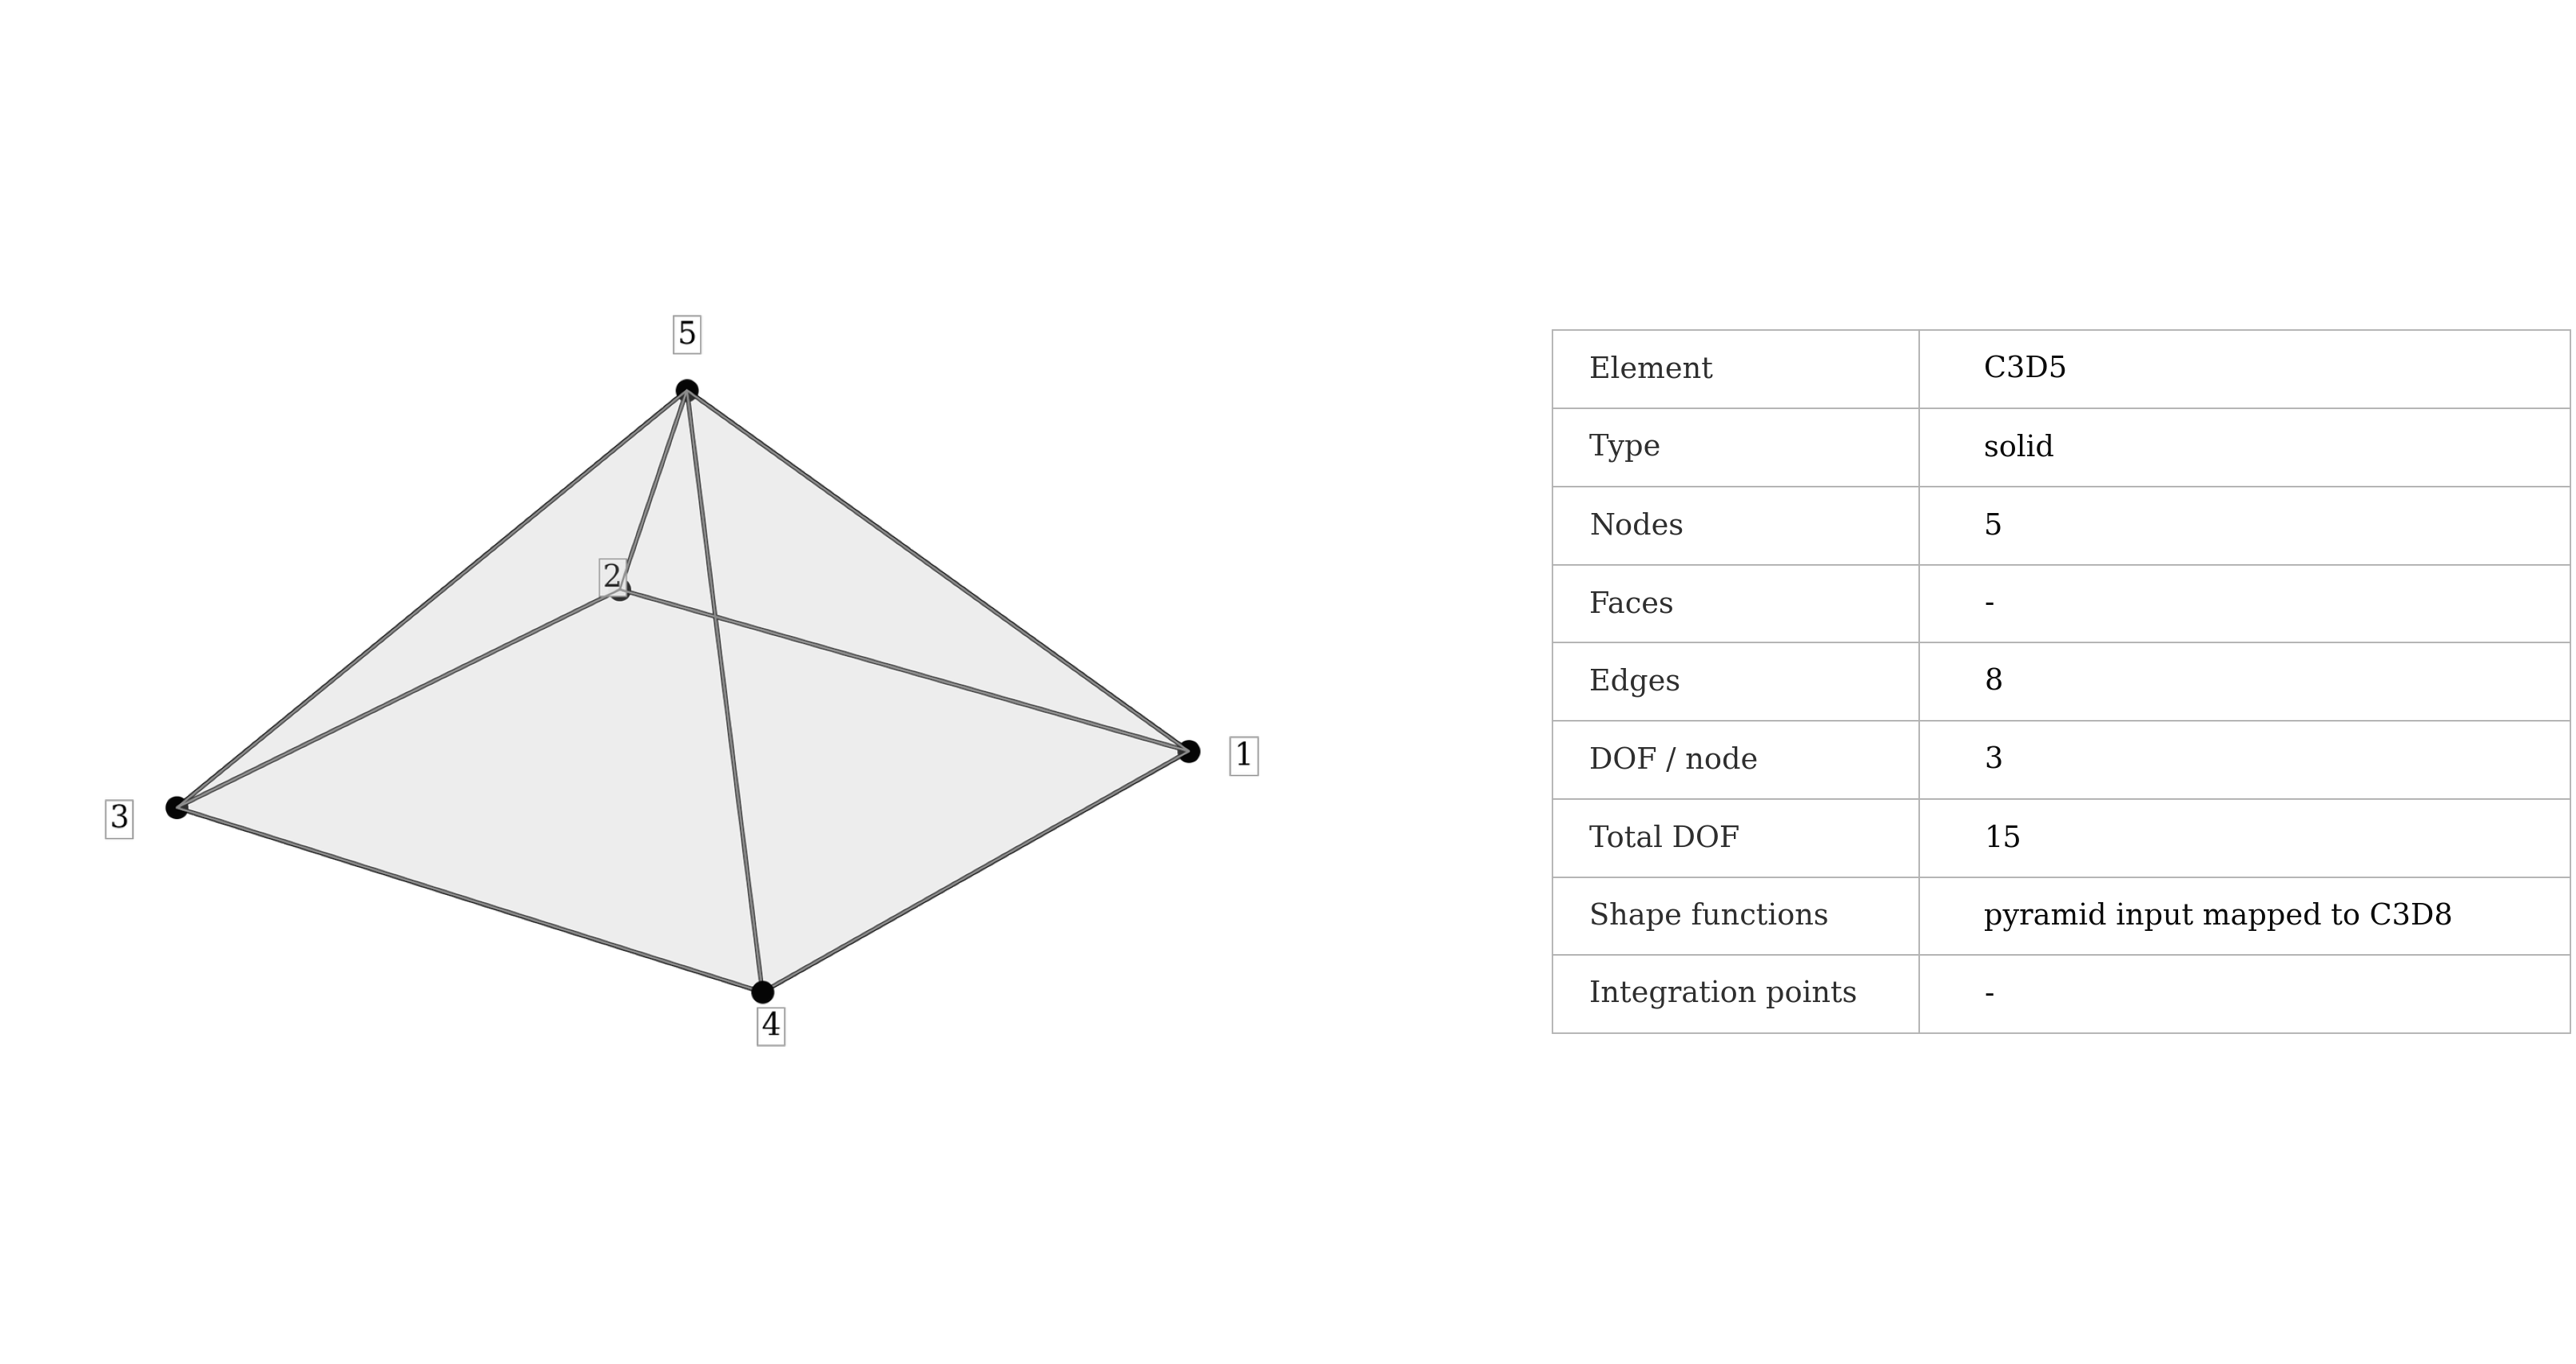
\includegraphics[width=0.78\linewidth]{pages/figures/element_schematics/c3d5_schematic.png}
    \caption{\val{C3D5} pyramid input topology.}
\end{figure}

\begin{syntax}
*ELEMENT, TYPE=C3D5, ELSET=<set>
<id>, <n1>, <n2>, <n3>, <n4>, <apex>
\end{syntax}

\val{C3D5} provides a five-node pyramid connectivity for transition meshes. FEMaster represents this input with a degenerated eight-node hexahedral topology in which the four upper hexahedral positions coincide at the pyramid apex. The user nevertheless writes the natural five-node pyramid connectivity shown above.

The element primarily acts as a transition cell between hexahedral and tetrahedral regions. In automatically generated mixed meshes, it connects a quadrilateral face to tetrahedral topology without forcing a large surrounding region to change element family.

A degenerated mapping is generally less predictable than a regular hexahedron, wedge, or tetrahedron. Flat pyramids, badly skewed bases, and apex positions close to the base plane can produce poor Jacobians and unreliable stiffness. These properties limit \val{C3D5} primarily to transition regions rather than large stress-critical volumes.

In models with many pyramids in the primary load path, reactions and global stiffness can remain plausible even when local stress quality differs significantly from an alternative regular-element mesh.

\clearpage
\paragraph{\val{C3D6}: 6-node wedge solid}

\begin{figure}[H]
    \centering
    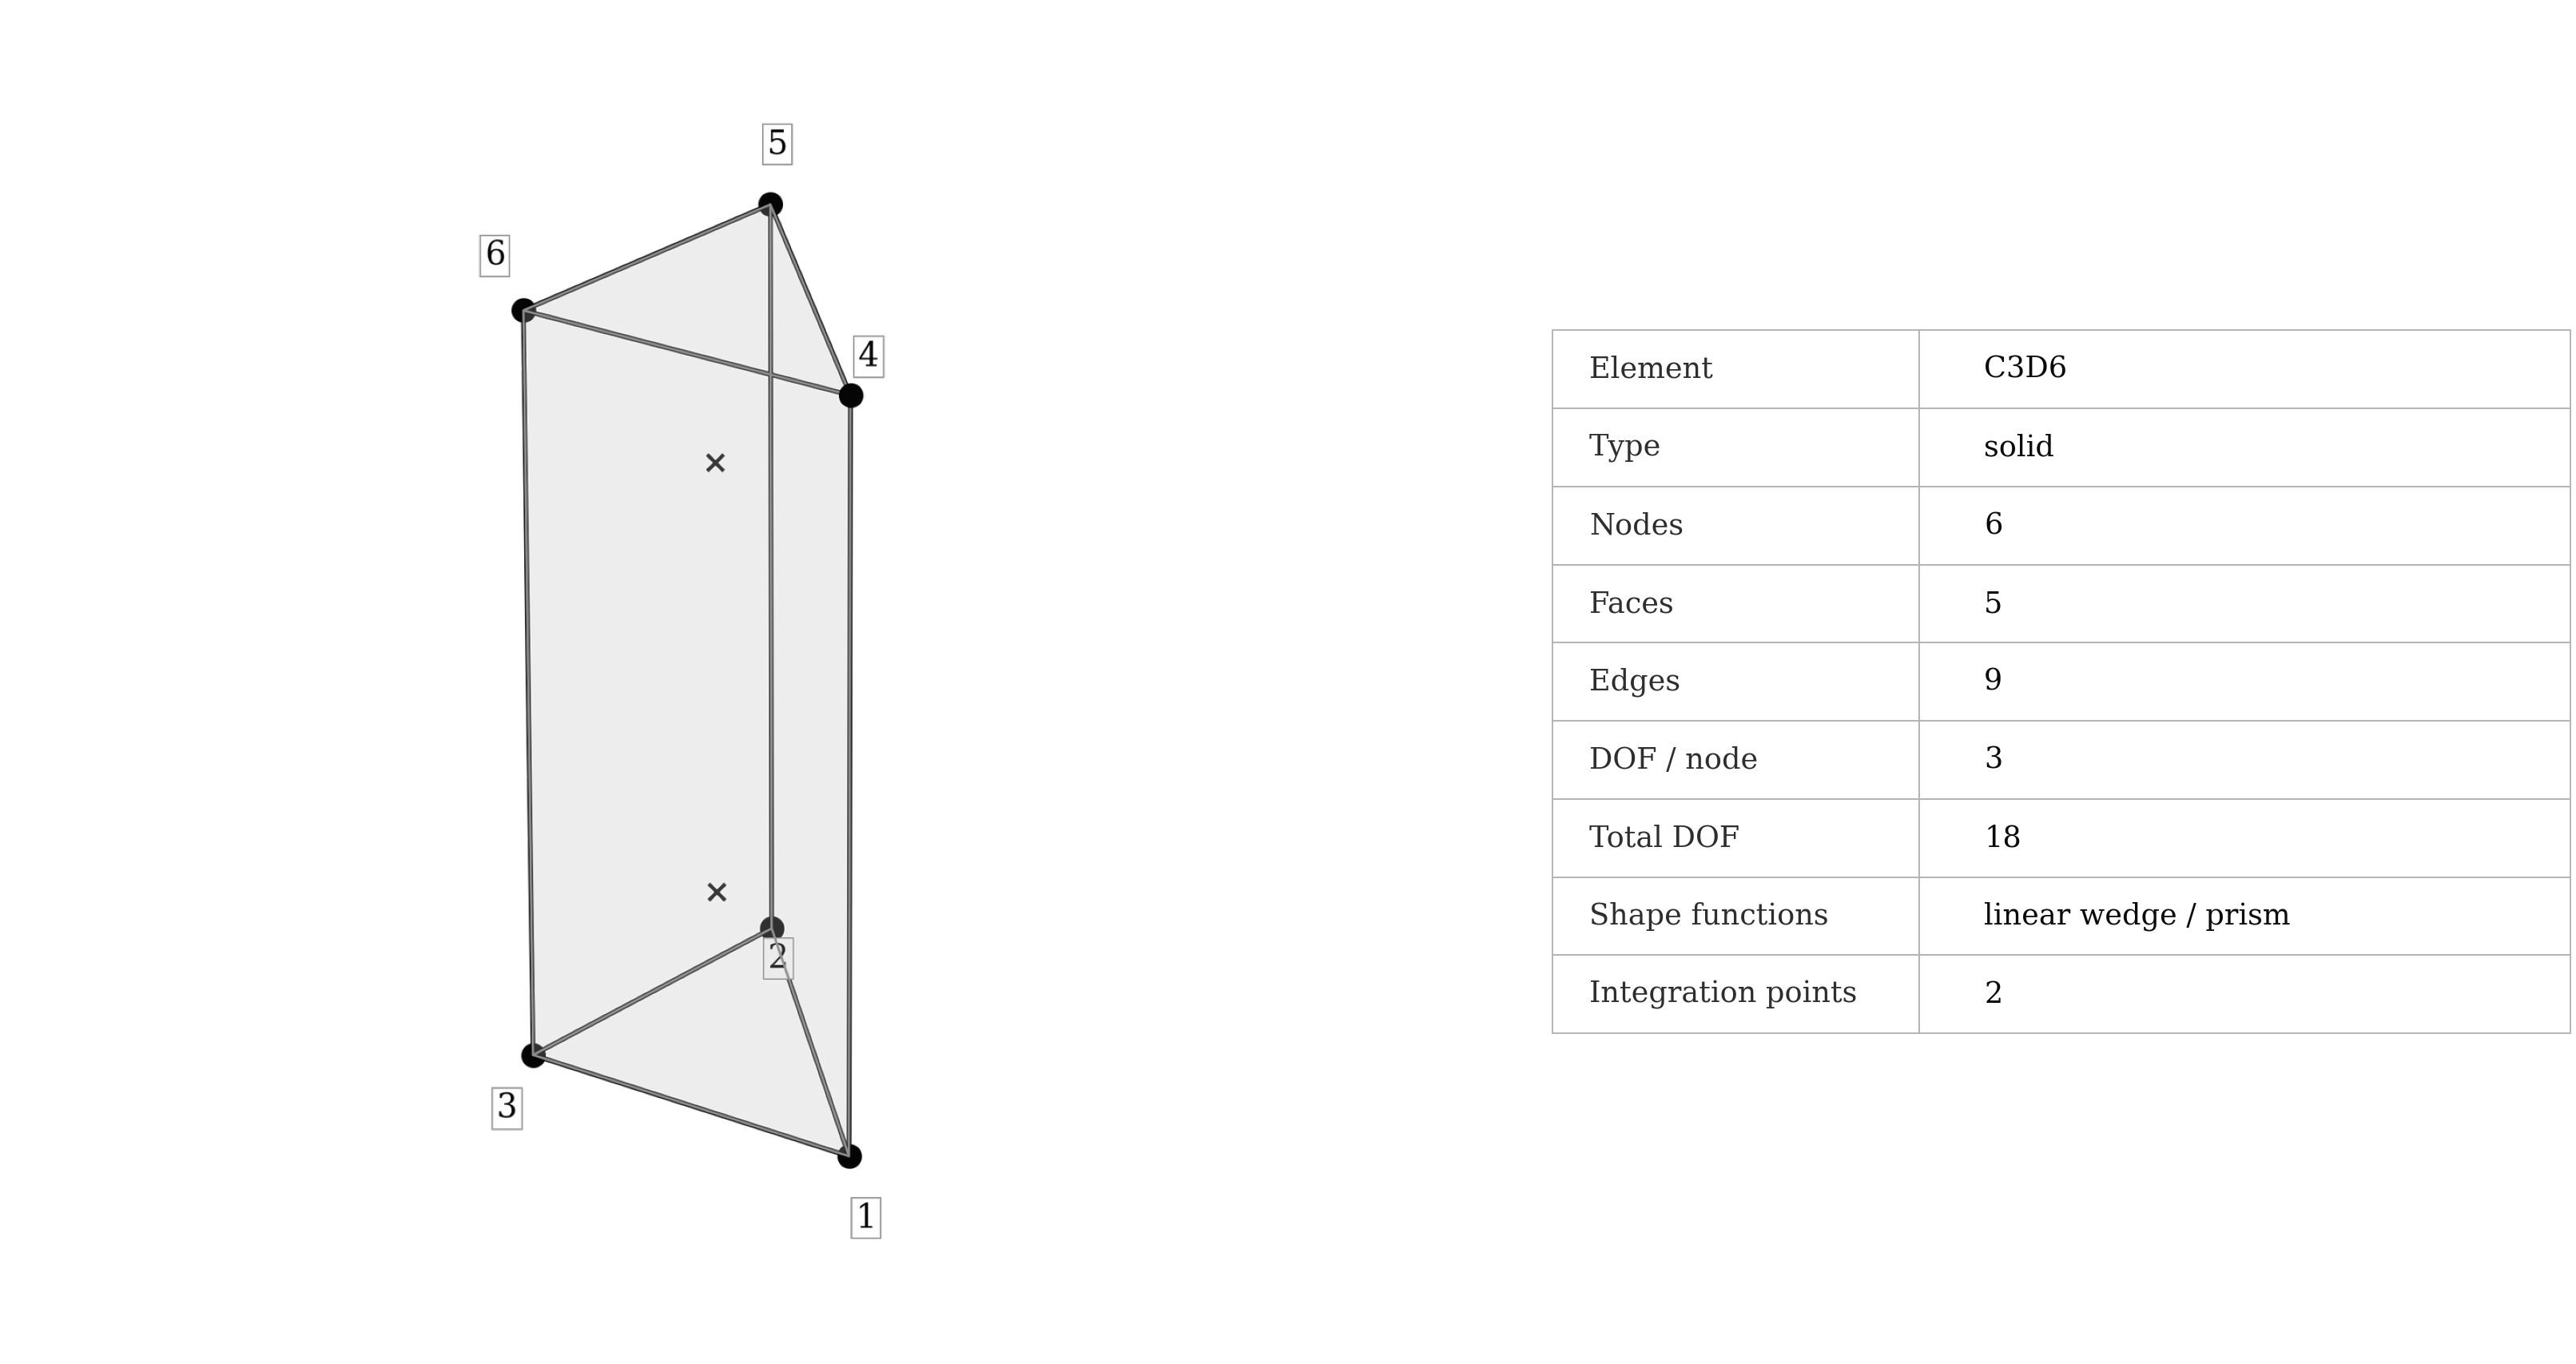
\includegraphics[width=0.78\linewidth]{pages/figures/element_schematics/c3d6_schematic.png}
    \caption{\val{C3D6} wedge element.}
\end{figure}

\begin{syntax}
*ELEMENT, TYPE=C3D6, ELSET=<set>
<id>, <n1>, <n2>, <n3>, <n4>, <n5>, <n6>
\end{syntax}

\val{C3D6} is a linear wedge or prism element. It combines triangular end faces with quadrilateral side faces and represents swept meshes, extruded triangular surface meshes, layered regions, and transitions where a purely hexahedral topology is not possible.

A wedge mesh can align naturally with a dominant through-thickness or extrusion direction. In locally layered solids and prismatic regions, its element rows can follow the physical geometry more consistently than an unstructured tetrahedral mesh.

Like other low-order elements, \val{C3D6} has limited bending and gradient resolution. One or two linear wedges through the thickness of a bending-dominated region provide limited stress recovery. Resolution increases with the number of elements in the gradient direction, while collapsed triangular faces, excessive twisting between end faces, and highly skewed side faces degrade the mapping.

\val{C3D6} matches geometries with a natural wedge topology. \val{C3D15} provides the corresponding higher-order interpolation for quadratic swept meshes.

\clearpage
\paragraph{\val{C3D8}: 8-node hexahedral solid}

\begin{figure}[H]
    \centering
    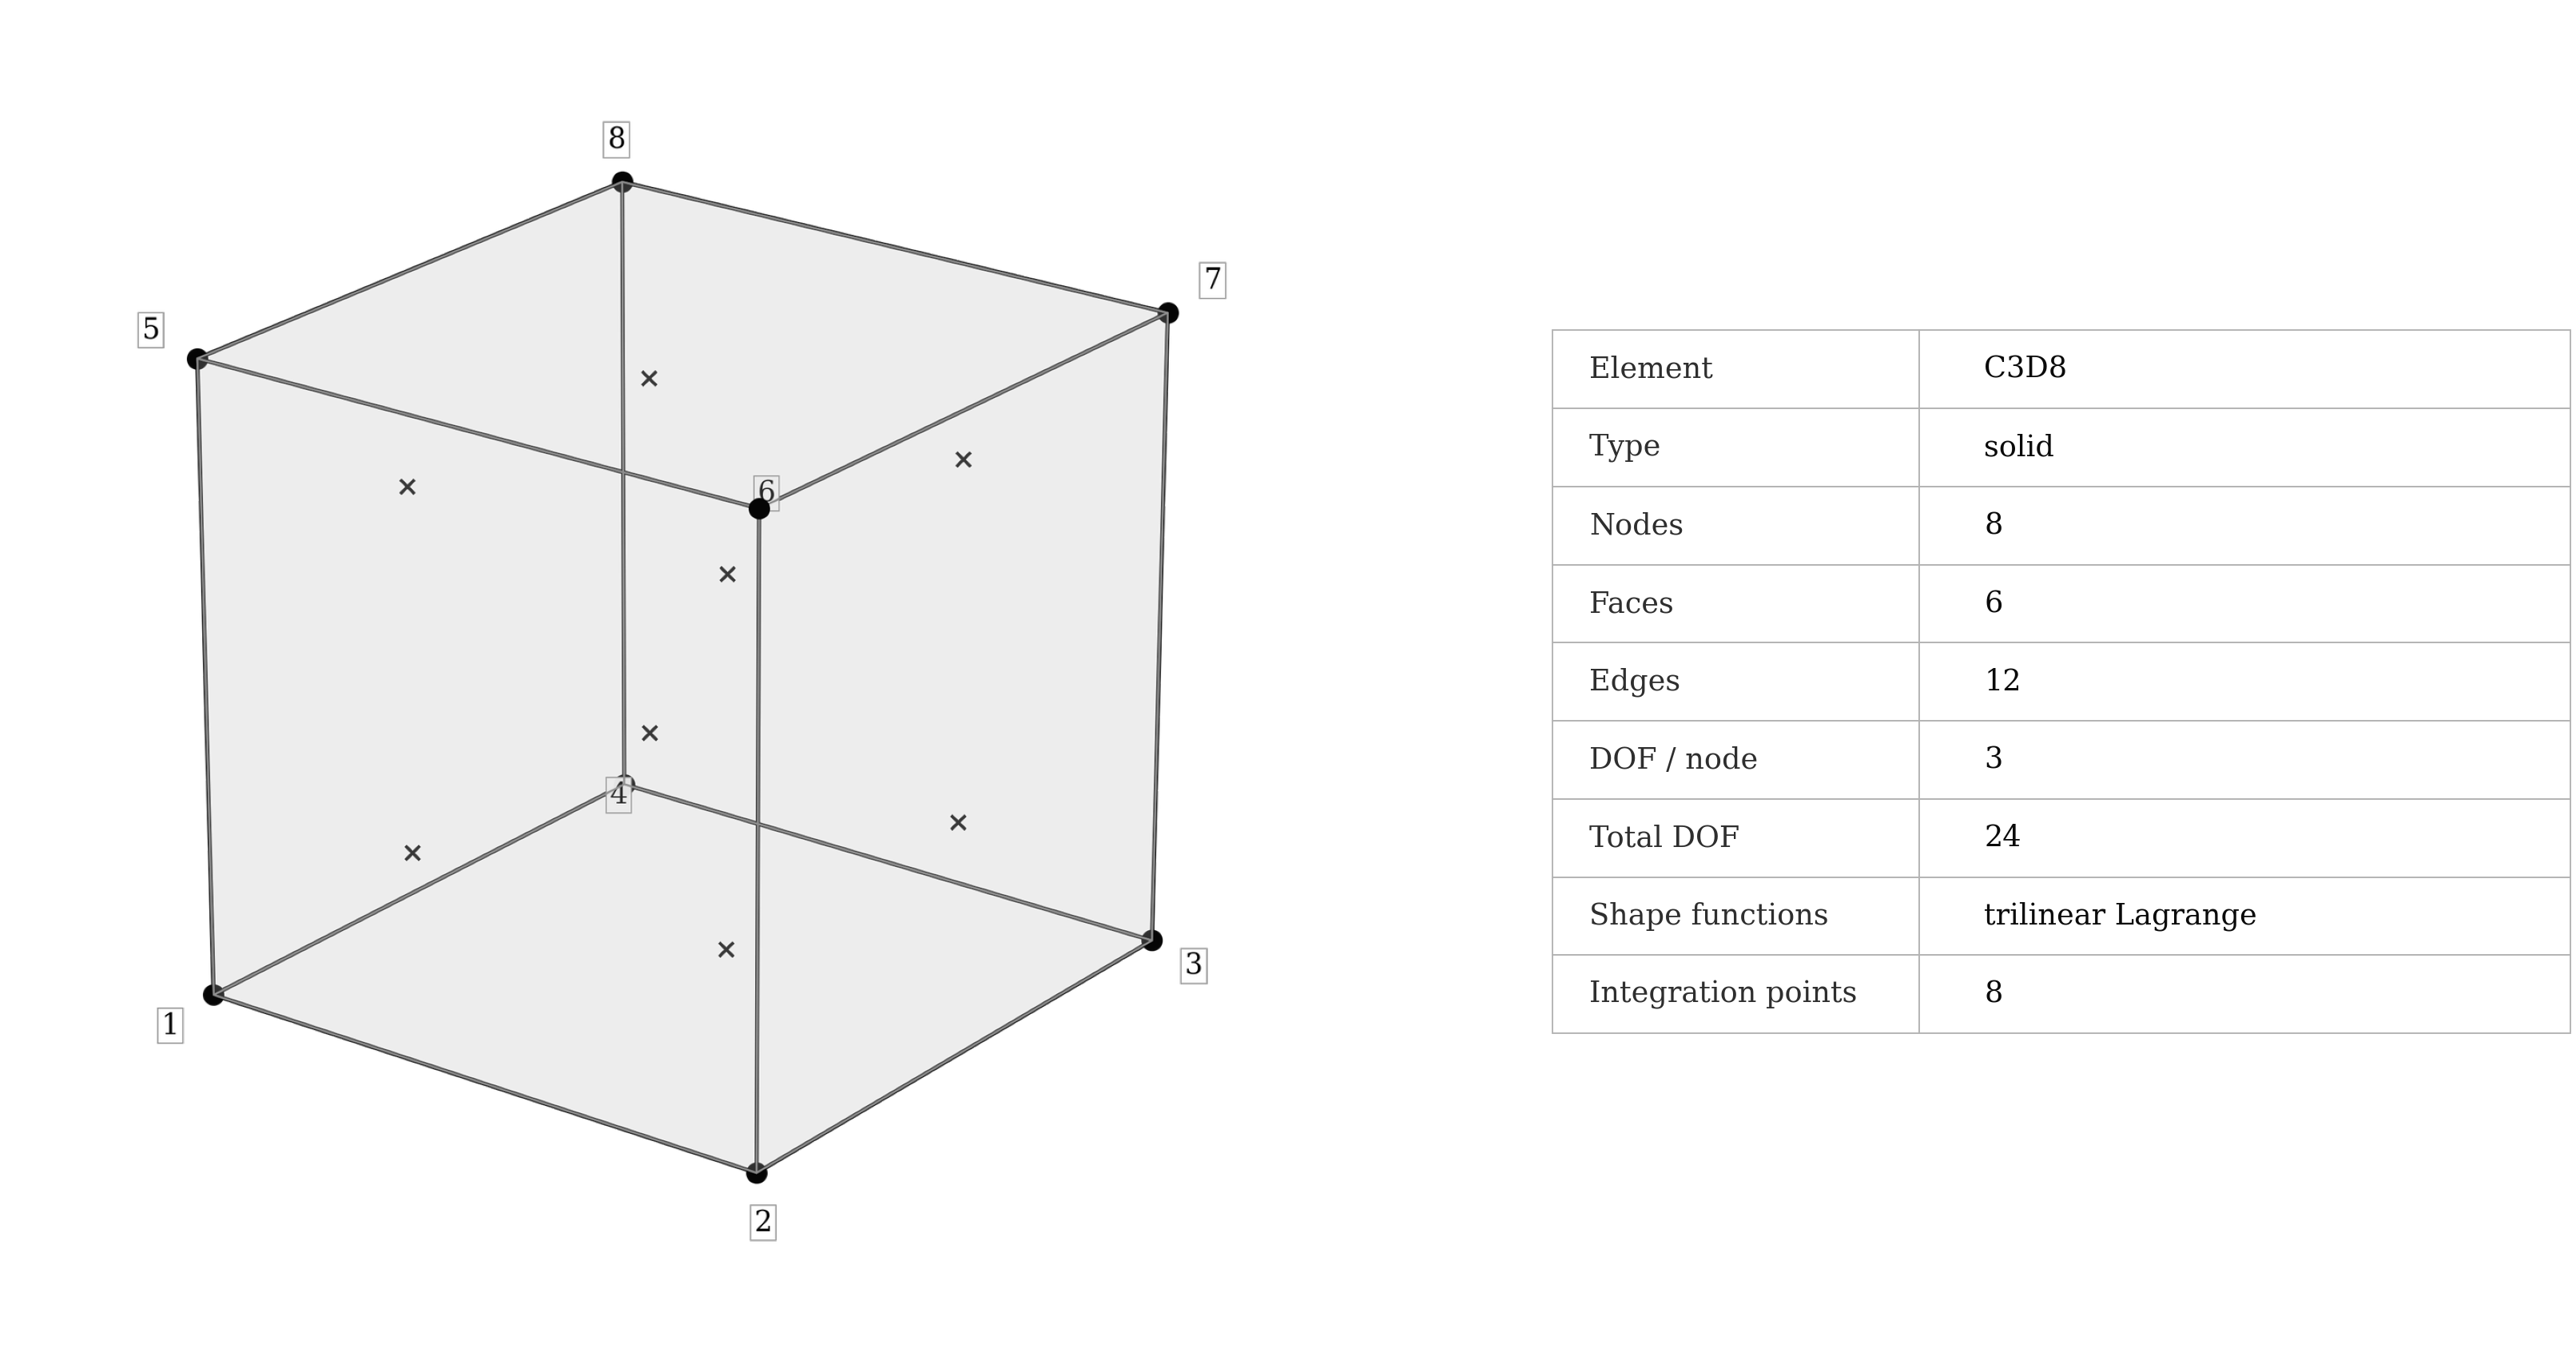
\includegraphics[width=0.82\linewidth]{pages/figures/element_schematics/c3d8_schematic.png}
    \caption{\val{C3D8} hexahedral solid element.}
\end{figure}

\begin{syntax}
*ELEMENT, TYPE=C3D8, ELSET=<set>
<id>, <n1>, <n2>, <n3>, <n4>, <n5>, <n6>, <n7>, <n8>
\end{syntax}

\val{C3D8} is the standard low-order hexahedral continuum element. It uses trilinear displacement interpolation and full integration. For regular block-like, swept, or layered meshes it is often an efficient general-purpose solid because element directions can follow geometry and material orientation naturally.

Hexahedral topology provides direct control of the number of elements through thickness and along structural load paths. A regular \val{C3D8} mesh therefore represents plates modelled with solids, bonded layers, spars, ribs, extruded components, and regions whose orthotropic material axes follow the mesh.

The element remains low order. A coarse mesh can be too stiff in bending, and straight element edges only approximate curved boundaries. Through-thickness resolution and refinement of curved or stress-critical geometry directly control the corresponding bending-stress and geometry errors.

Warping, skew, negative Jacobians, and extreme aspect ratios can remove the numerical advantages of the hexahedral topology. A clean quadratic tetrahedral mesh can provide a more accurate mapping than a badly distorted hexahedral mesh; topology alone does not determine mesh quality.

\clearpage
\paragraph{\val{C3D8I}: incompatible-mode 8-node hexahedral solid}

\begin{figure}[H]
    \centering
    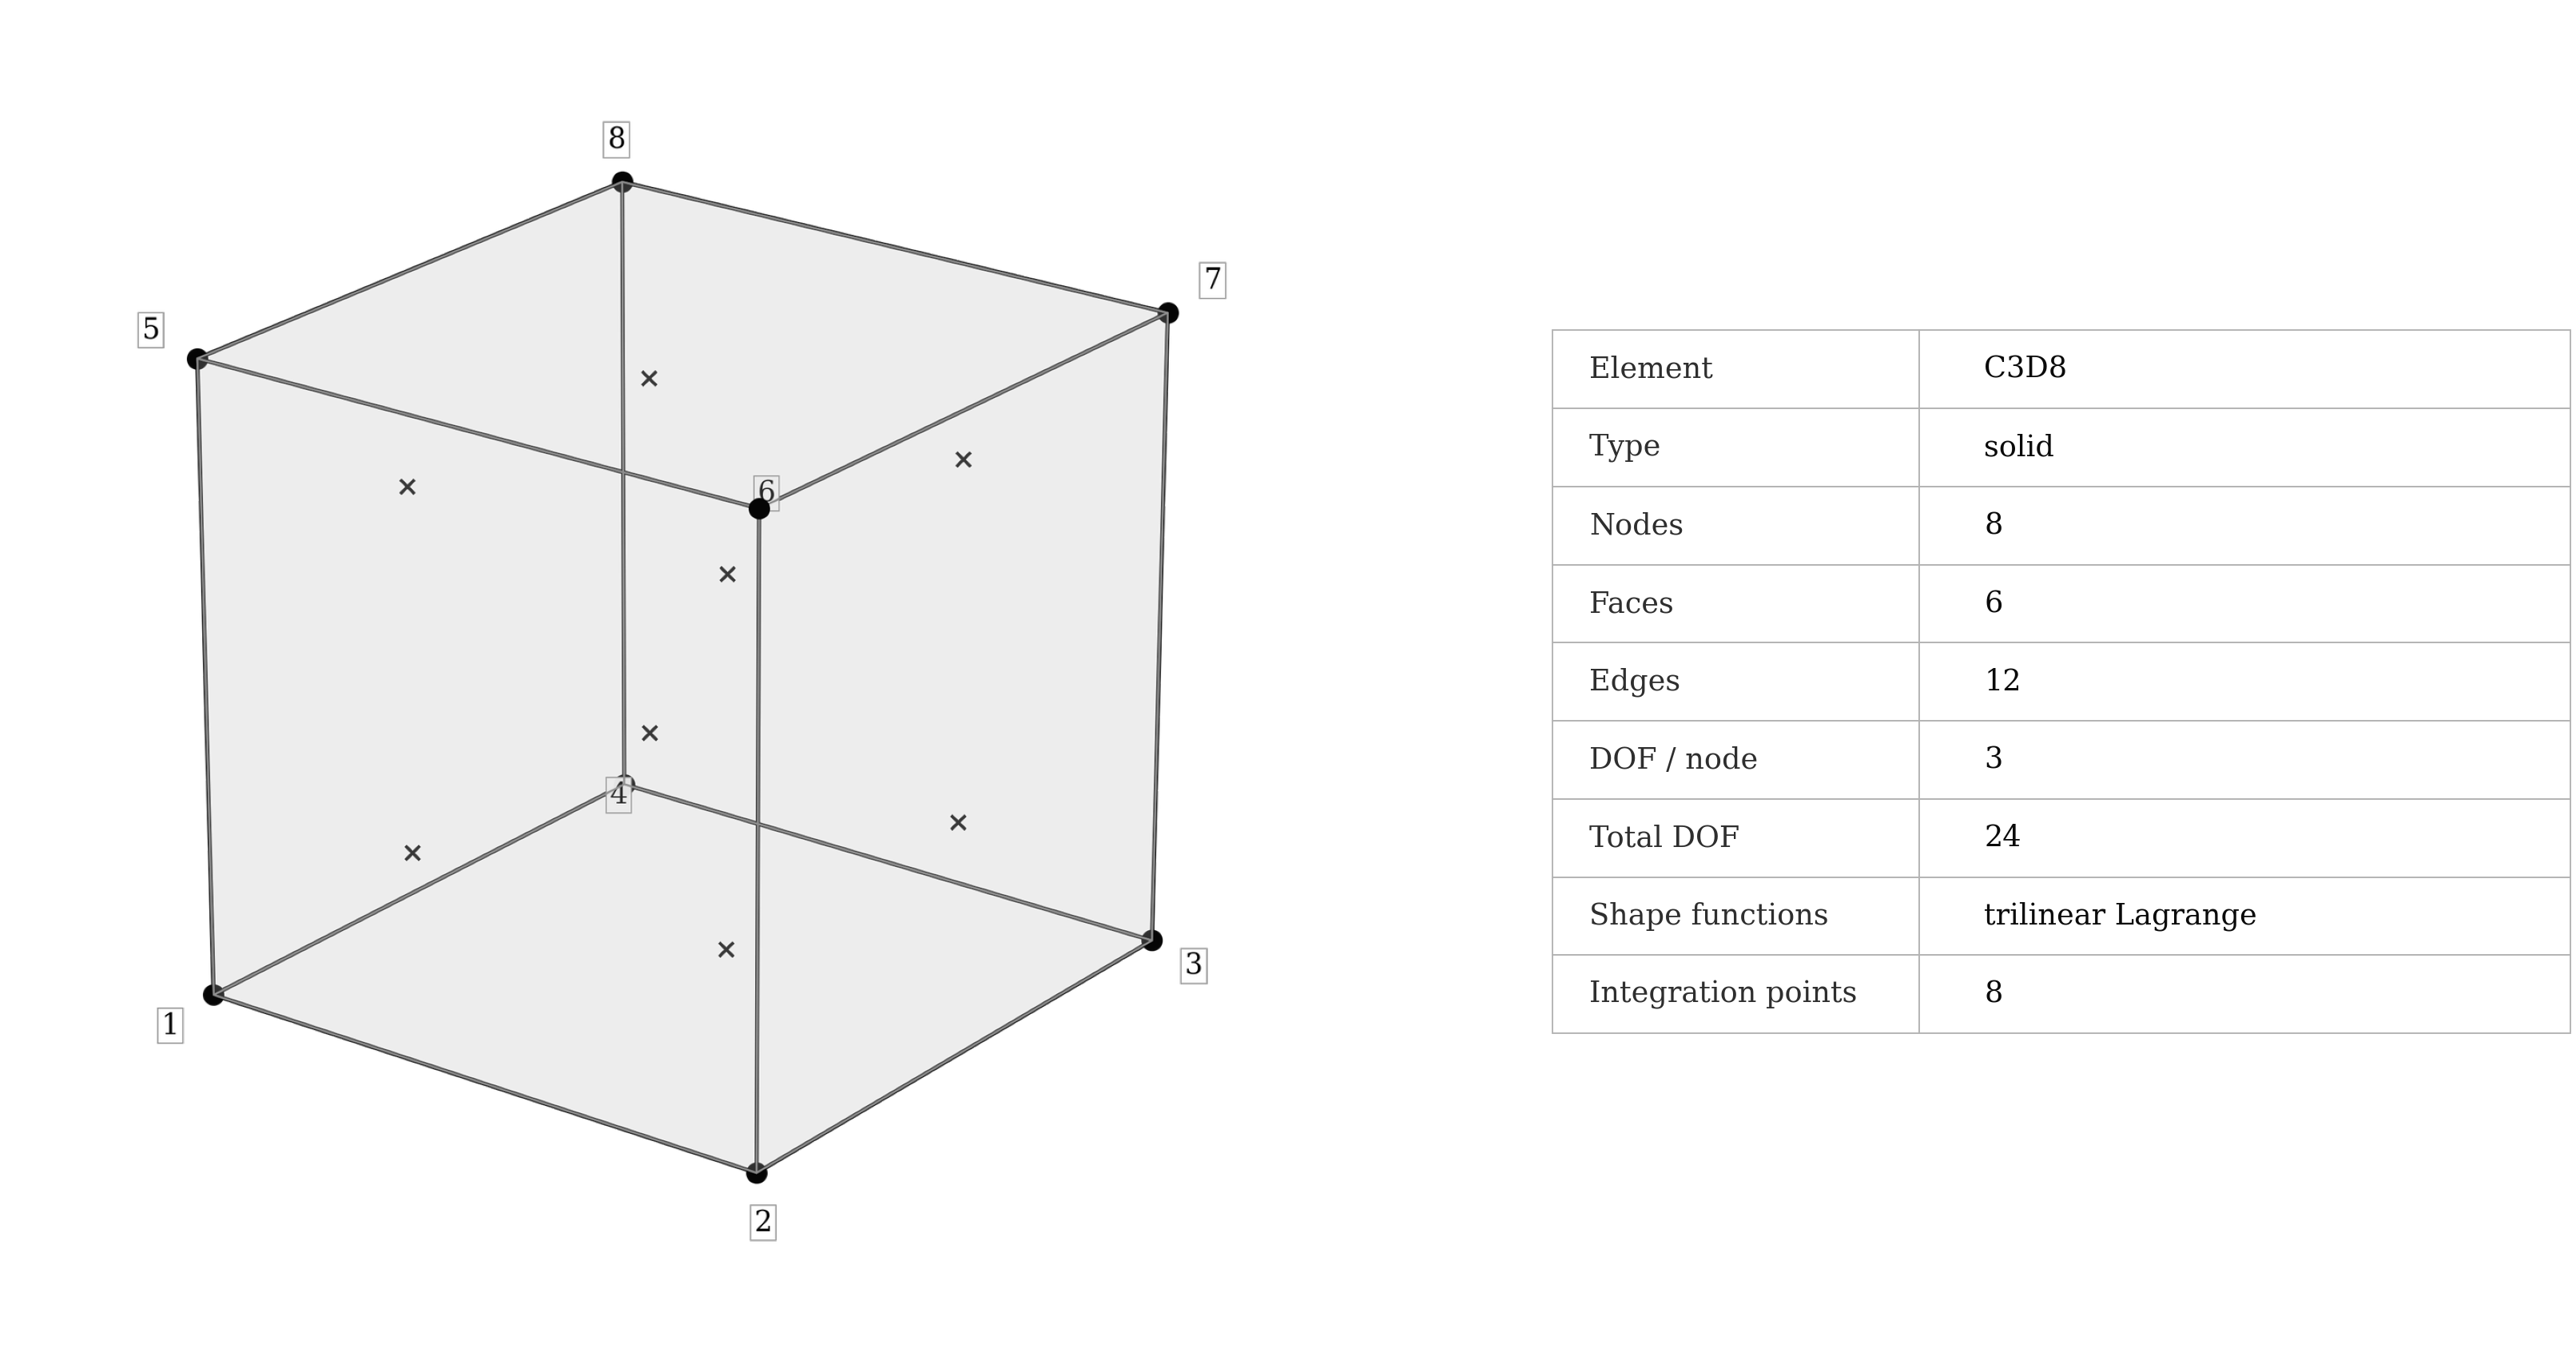
\includegraphics[width=0.82\linewidth]{pages/figures/element_schematics/c3d8_schematic.png}
    \caption{\val{C3D8I} topology; the eight external nodes are identical to \val{C3D8}.}
\end{figure}

\begin{syntax}
*ELEMENT, TYPE=C3D8I, ELSET=<set>
<id>, <n1>, <n2>, <n3>, <n4>, <n5>, <n6>, <n7>, <n8>
\end{syntax}

\val{C3D8I} uses the same trilinear eight-node geometry and the same full
\(2\times2\times2\) integration rule as \val{C3D8}. Its compatible displacement
field is augmented by 13 element-local enhanced modes. Nine principal
vector-valued modes improve bending behaviour by removing parasitic constraints
of the low-order compatible interpolation; four additional volumetric modes
improve the response in nearly incompressible states.

The 13 enhanced parameters are internal to each element. FEMaster solves their
local stationarity equations and statically condenses them, so a \val{C3D8I}
still contributes only the 24 translational nodal degrees of freedom of an
ordinary eight-node solid to the global system. Unlike \val{C3D8R}, the element
does not rely on reduced integration or hourglass stabilization.

For geometrically nonlinear analysis the enhanced parameters are solved by a
local Newton iteration at every element evaluation and the complete material and
geometric tangent blocks are condensed by a Schur complement. The finite-strain
kinematics use a right multiplicative enhancement
\[
\bar{\mathbf F}
=
\mathbf F_c
\left(
\mathbf I + \sum_m \alpha_m \mathbf H_m
\right).
\]
The enhanced tensors therefore remain in the reference configuration. A
superposed spatial rigid rotation maps
\(\bar{\mathbf F}\rightarrow\mathbf Q\bar{\mathbf F}\), so the enhanced
mode space and condensed response remain objective.

\val{C3D8I} is intended primarily for low-order hexahedral meshes in which
bending or near-incompressibility makes a standard \val{C3D8} unnecessarily
stiff. It remains a trilinear geometry mapping and is still sensitive to severe
warping and skew. The incompatible modes improve the kinematics; they do not turn
a poor eight-node geometry into a higher-order element.

\clearpage
\paragraph{\val{C3D8R}: reduced-integration 8-node hexahedral solid}

\begin{figure}[H]
    \centering
    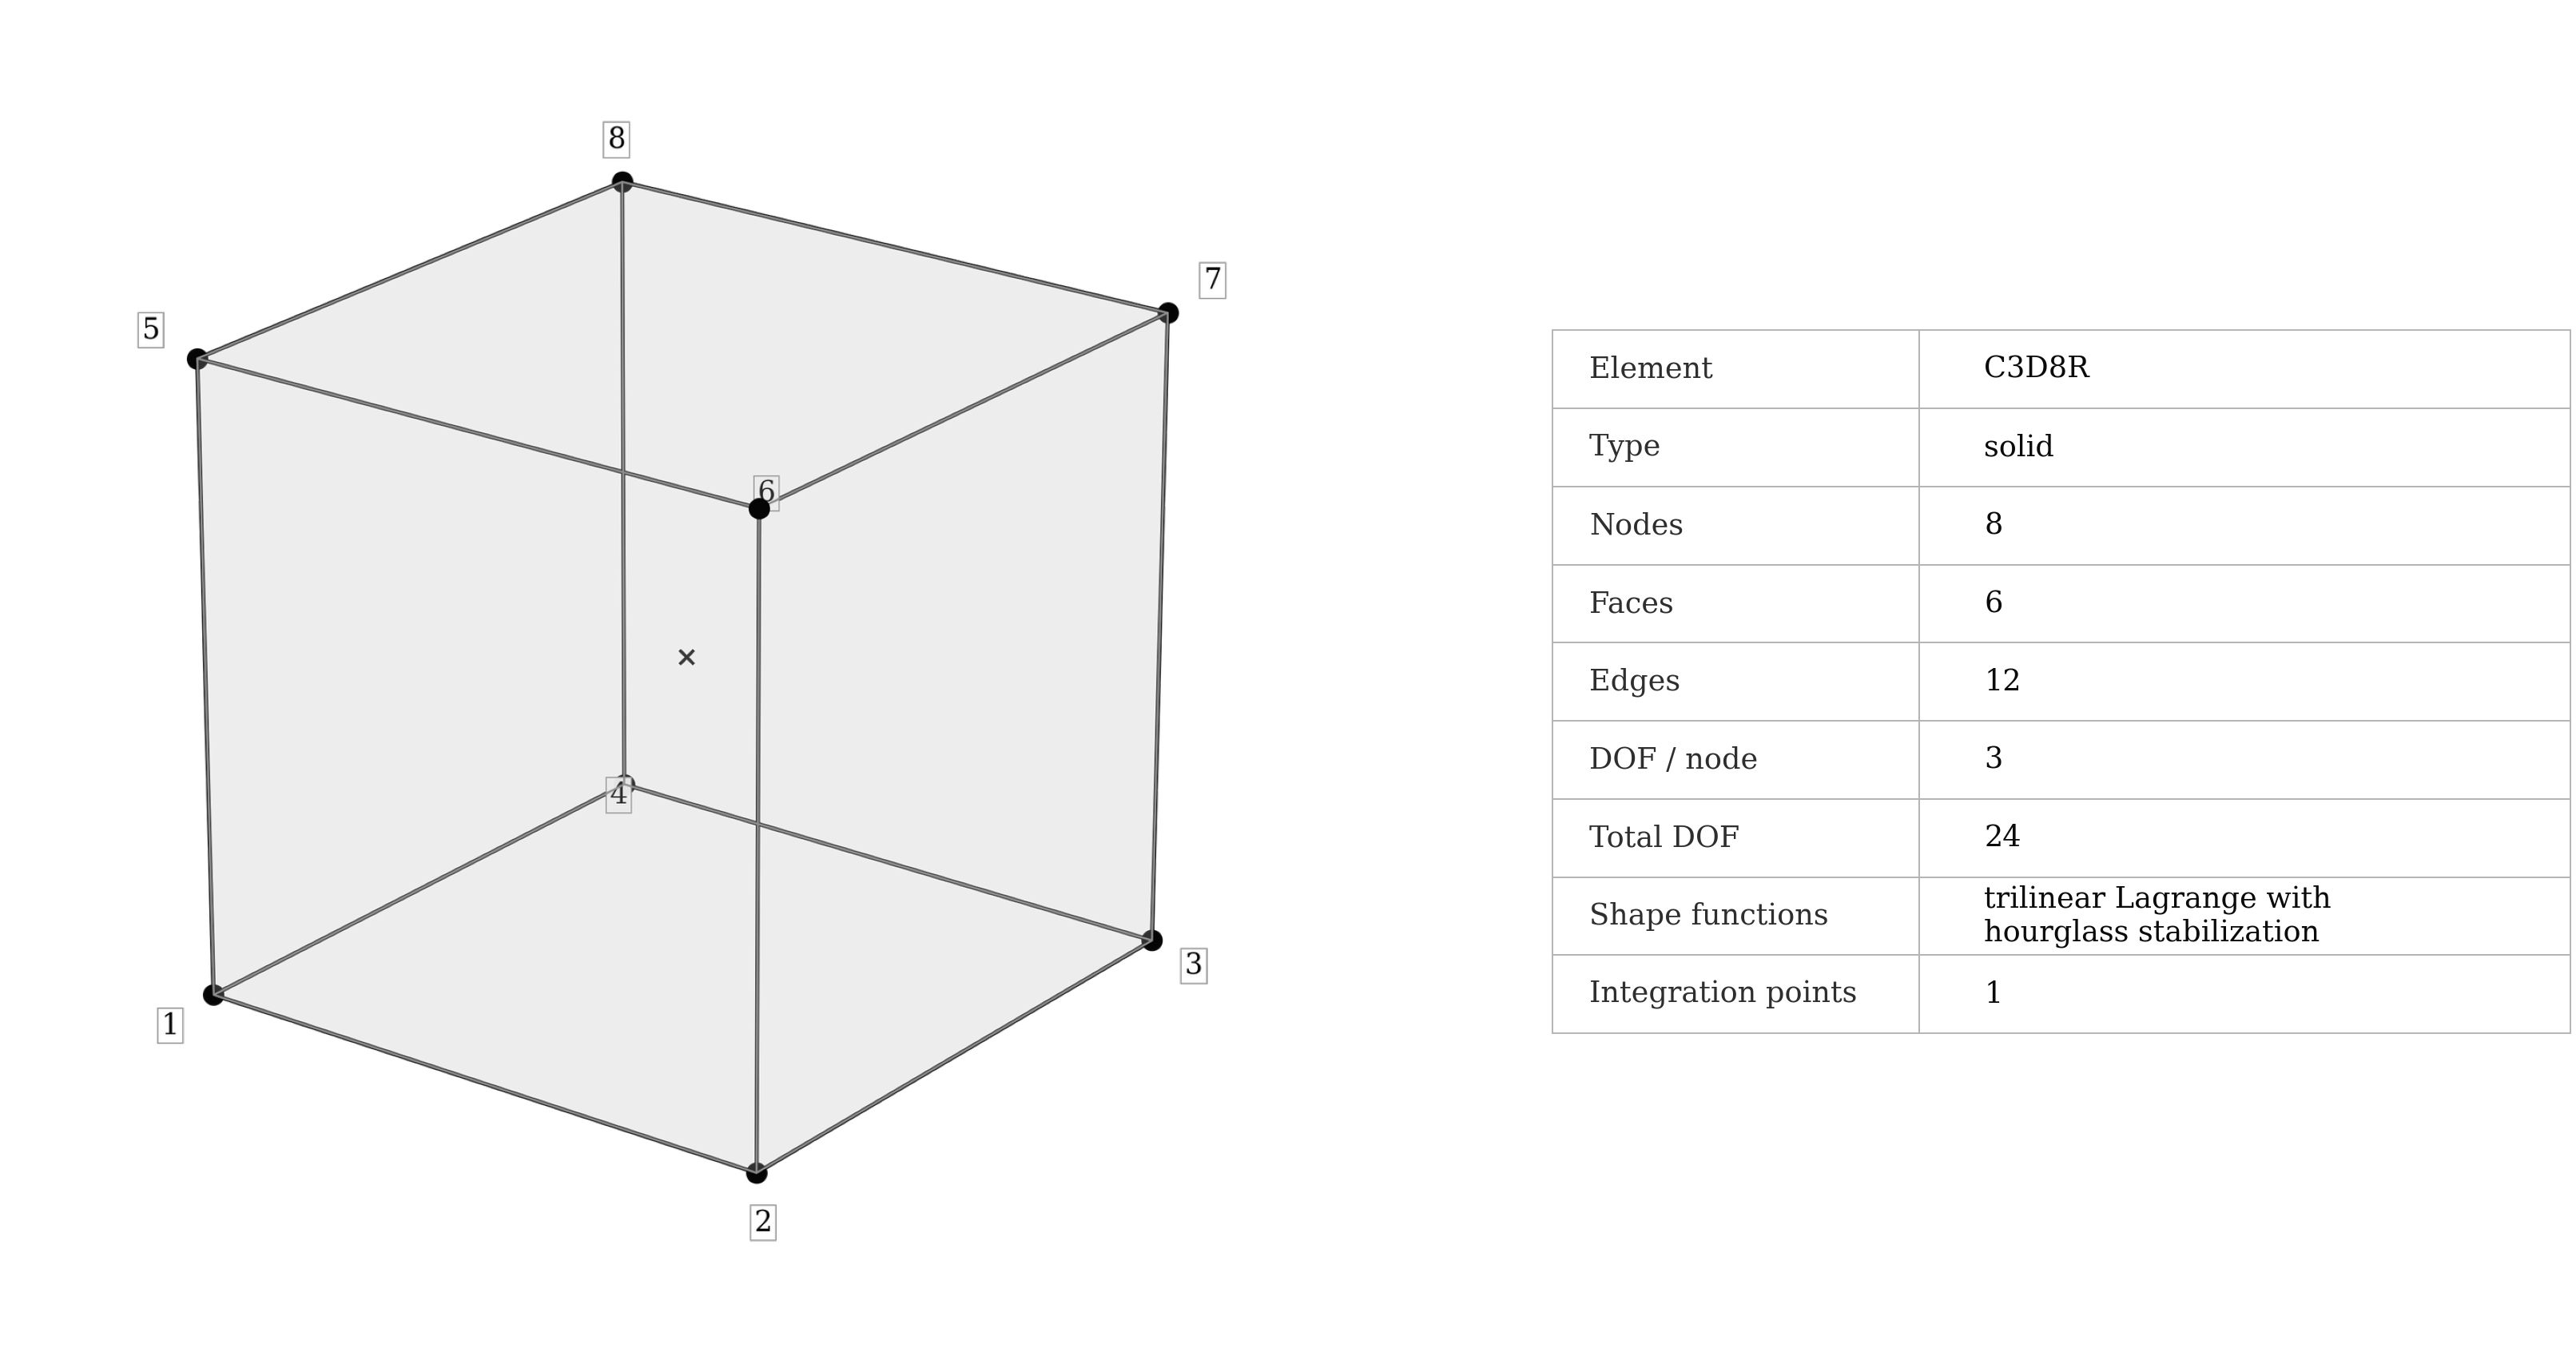
\includegraphics[width=0.82\linewidth]{pages/figures/element_schematics/c3d8r_schematic.png}
    \caption{\val{C3D8R} reduced-integration hexahedral solid element.}
\end{figure}

\begin{syntax}
*ELEMENT, TYPE=C3D8R, ELSET=<set>
<id>, <n1>, <n2>, <n3>, <n4>, <n5>, <n6>, <n7>, <n8>
\end{syntax}

\val{C3D8R} uses the same eight-node topology as \val{C3D8} but evaluates the continuum contribution with one integration point at the element centre. Reduced integration lowers assembly cost and avoids some of the excessive stiffness that a fully integrated low-order hexahedron can exhibit in bending-dominated states.

One-point integration also introduces zero-energy hourglass deformation modes. FEMaster therefore adds hourglass stabilization. The primitive scalar hourglass patterns are based on the four non-affine modes
\[
\gamma_1=s\,t,\qquad
\gamma_2=t\,r,\qquad
\gamma_3=r\,s,\qquad
\gamma_4=r\,s\,t.
\]
These modes are projected so that affine displacement fields are not penalized. The stabilization scale is based on the element reference volume, the reference geometry gradients, and an effective shear stiffness derived from the constitutive tangent. The default dimensionless hourglass coefficient is \(\alpha=0.005\).

Newton convergence alone does not characterize \val{C3D8R}; the deformation pattern and stabilization sensitivity are independent numerical properties. A coarse or badly distorted mesh can converge while exhibiting nonphysical hourglass deformation. Comparison with \val{C3D8} and mesh refinement expose response components associated with hourglass-sensitive deformation.

Severe finite rotations and highly distorted elements increase sensitivity to reduced-integration stabilization. Relative to \val{C3D8}, \val{C3D8R} exchanges lower integration cost and locking tendency for dependence on hourglass control.

\clearpage
\paragraph{\val{C3D10}: 10-node quadratic tetrahedral solid}

\begin{figure}[H]
    \centering
    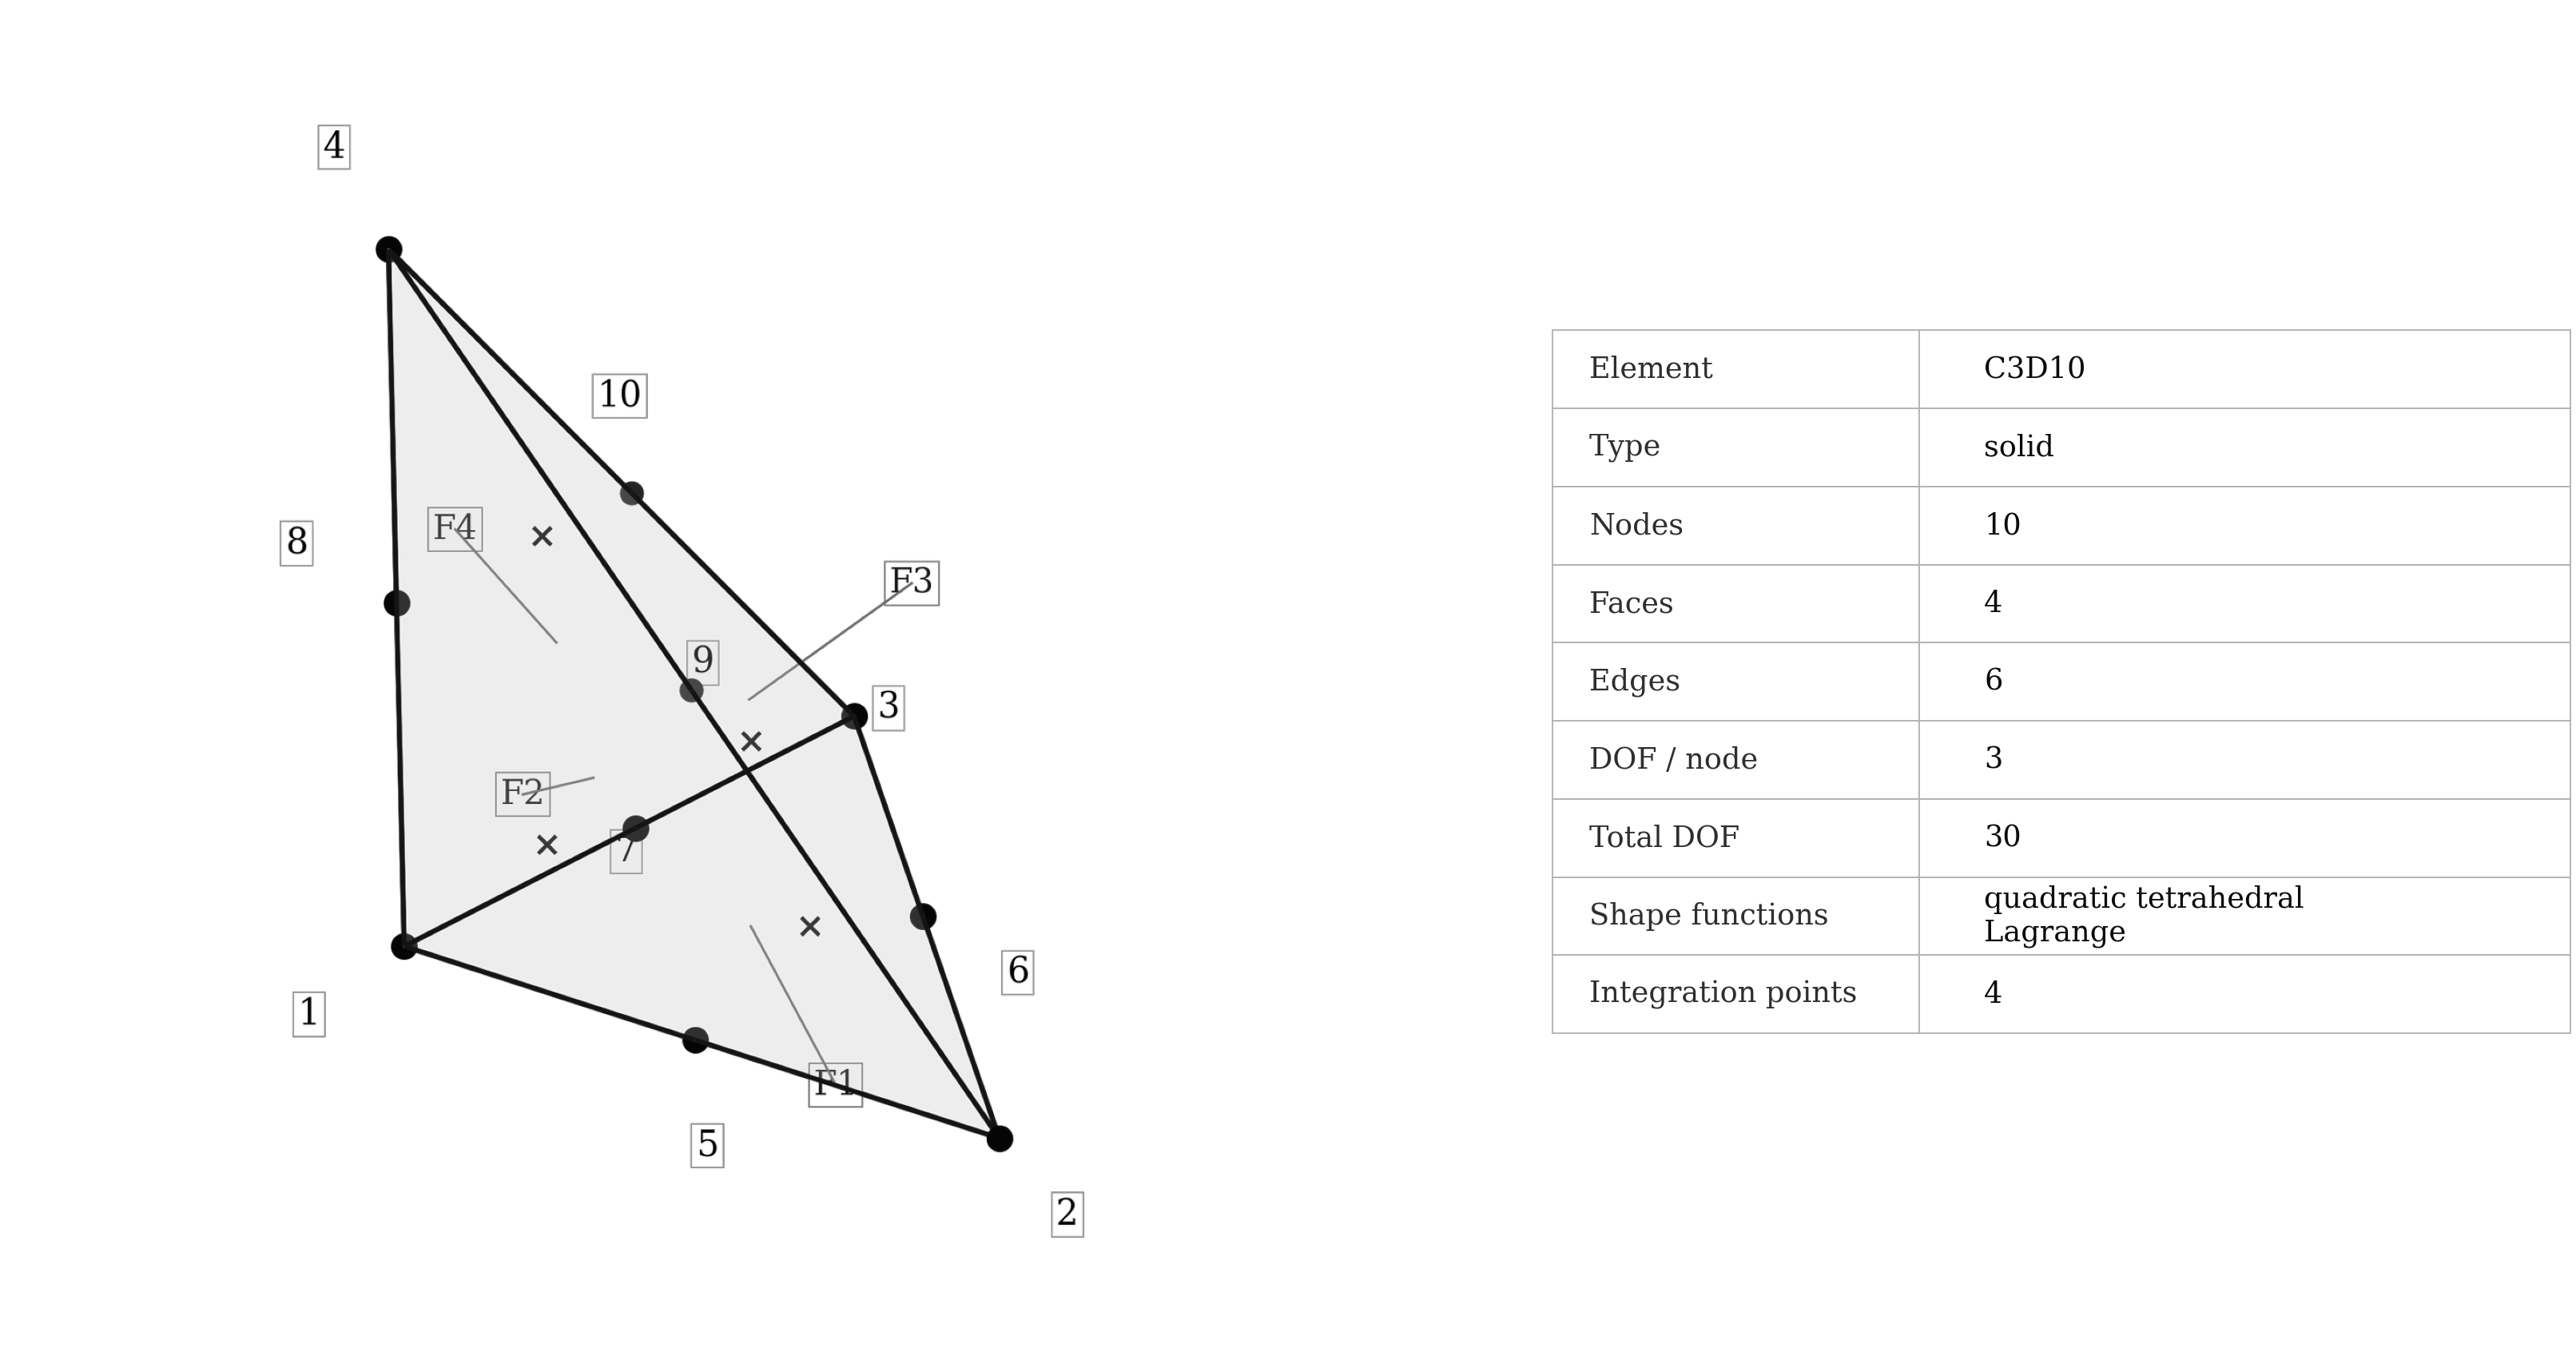
\includegraphics[width=0.80\linewidth]{pages/figures/element_schematics/c3d10_schematic.png}
    \caption{\val{C3D10} quadratic tetrahedral element.}
\end{figure}

\begin{syntax}
*ELEMENT, TYPE=C3D10, ELSET=<set>
<id>, <n1>, <n2>, <n3>, <n4>, <n5>, <n6>, <n7>, <n8>, <n9>, <n10>
\end{syntax}

\val{C3D10} is the quadratic tetrahedral solid. Six midside nodes augment the four corner nodes and allow quadratic displacement interpolation. Compared with \val{C3D4}, the element can represent curved deformation, bending, and stress gradients far more efficiently.

For automatic tetrahedral meshing, \val{C3D10} retains the geometric flexibility of tetrahedra while reducing the excessive stiffness and piecewise-constant strain behaviour associated with linear tetrahedra.

The quadratic geometry mapping also represents curved boundaries more accurately when midside nodes follow the CAD geometry. Badly displaced midside nodes can create a distorted mapping even if the corner tetrahedron appears acceptable.

The element costs more per cell than \val{C3D4}, but substantially fewer cells may be required for comparable displacement and stress accuracy. Refinement is still required near singularities, sharp re-entrant corners, and concentrated loads where no polynomial element can make a mathematical singularity disappear.

\clearpage
\paragraph{\val{C3D13}: 13-node quadratic pyramid solid}

\begin{figure}[H]
    \centering
    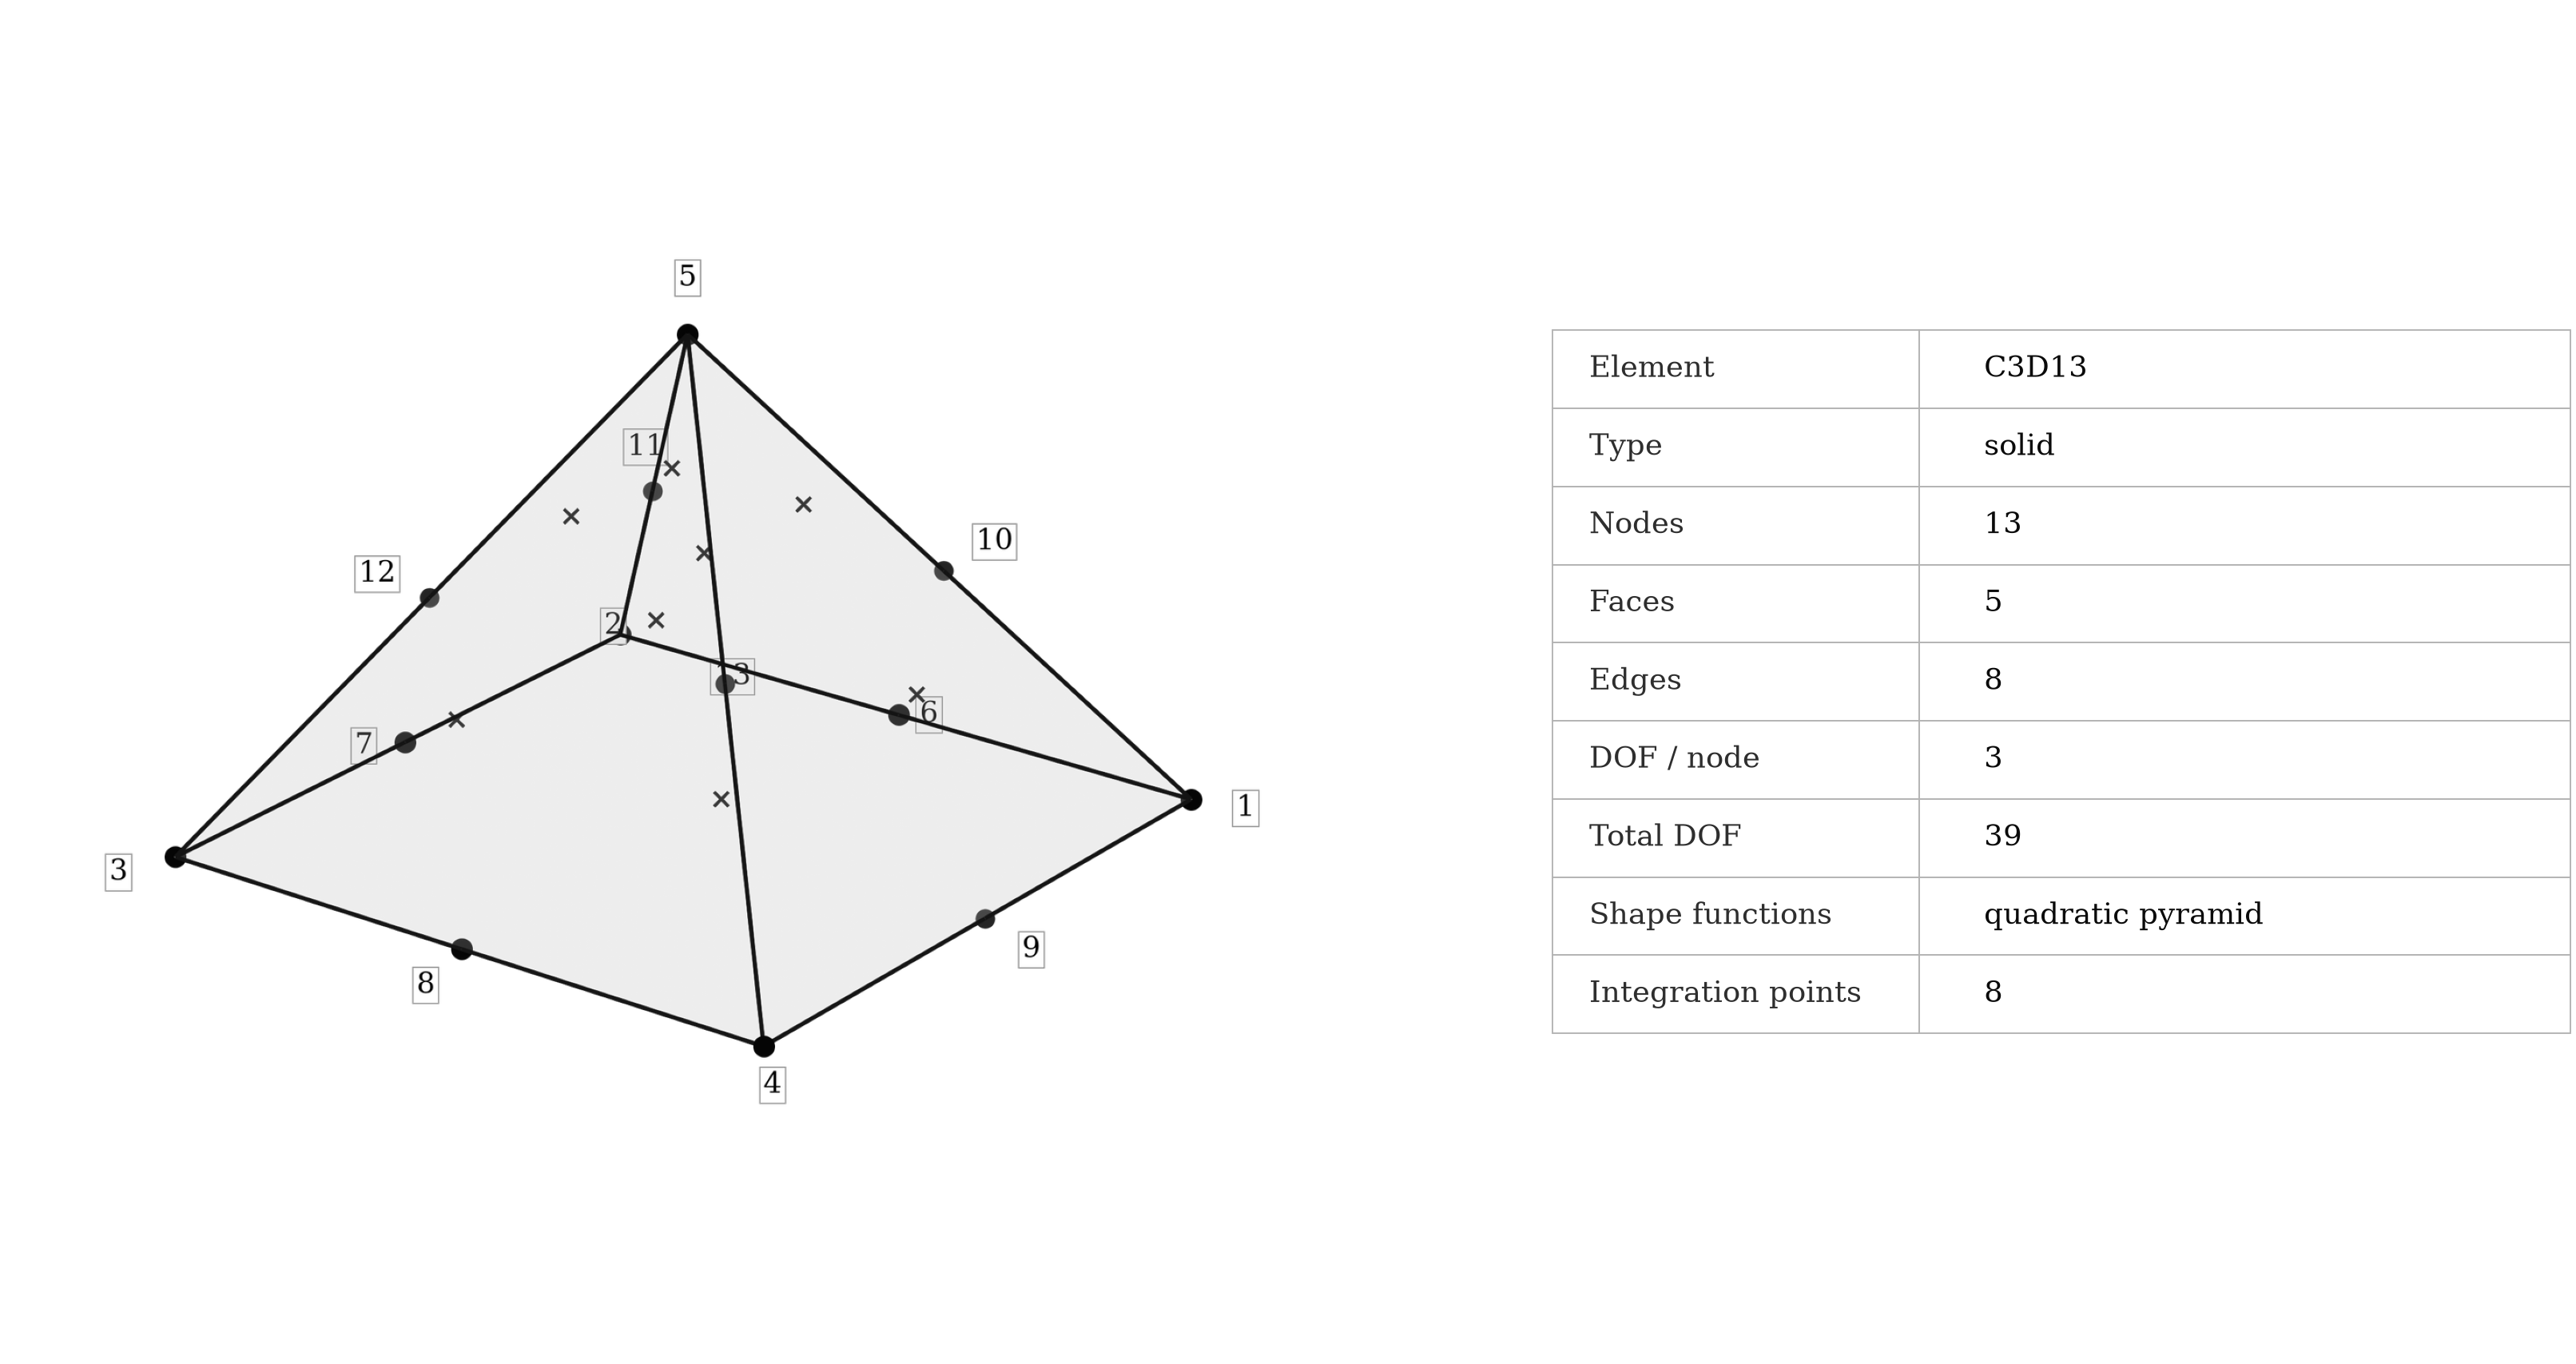
\includegraphics[width=0.78\linewidth]{pages/figures/element_schematics/c3d13_schematic.png}
    \caption{\val{C3D13} quadratic pyramid topology and integration scheme.}
\end{figure}

\begin{syntax}
*ELEMENT, TYPE=C3D13, ELSET=<set>
<id>, <n1>, <n2>, <n3>, <n4>, <n5>, <n6>, <n7>, <n8>, <n9>, <n10>, <n11>, <n12>, <n13>
\end{syntax}

\val{C3D13} is a thirteen-node quadratic pyramid element with rational
shape functions in the natural pyramid coordinates. Nodes 1--4 define
the quadrilateral base and node 5 the apex. Nodes 6--9 lie on the four
base edges, while nodes 10--13 lie between the base corners and the
apex. The rational interpolation accommodates the collapsed pyramid
geometry and provides a higher-order displacement description than
the five-node \val{C3D5} transition element.

A pyramid is useful where a quadrilateral-faced hexahedral mesh must
transition to a region containing tetrahedral cells. Compared with
\val{C3D5}, the midside nodes can represent curved edges and varying
deformation fields more accurately, provided their positions are
consistent with the intended physical geometry. Strongly distorted
pyramids or poor apex placement can still result in inaccurate
Jacobians, stiffness, and stress recovery.

The element uses the \val{DOMAIN_ISO_PYRAMID} quadrature with
\val{ORDER_QUARTIC} (27 integration points) and provides five
outward-oriented quadratic faces for surface definitions: an
eight-node quadrilateral base (\val{S1}) and four six-node
triangular sides (\val{S2}--\val{S5}). Recovered stress and strain
values are extrapolated from the constitutive integration points.
As for other quadratic solids, local stresses should be assessed
through mesh refinement rather than a single extrapolated nodal peak.

\clearpage
\paragraph{\val{C3D15}: 15-node quadratic wedge solid}

\begin{figure}[H]
    \centering
    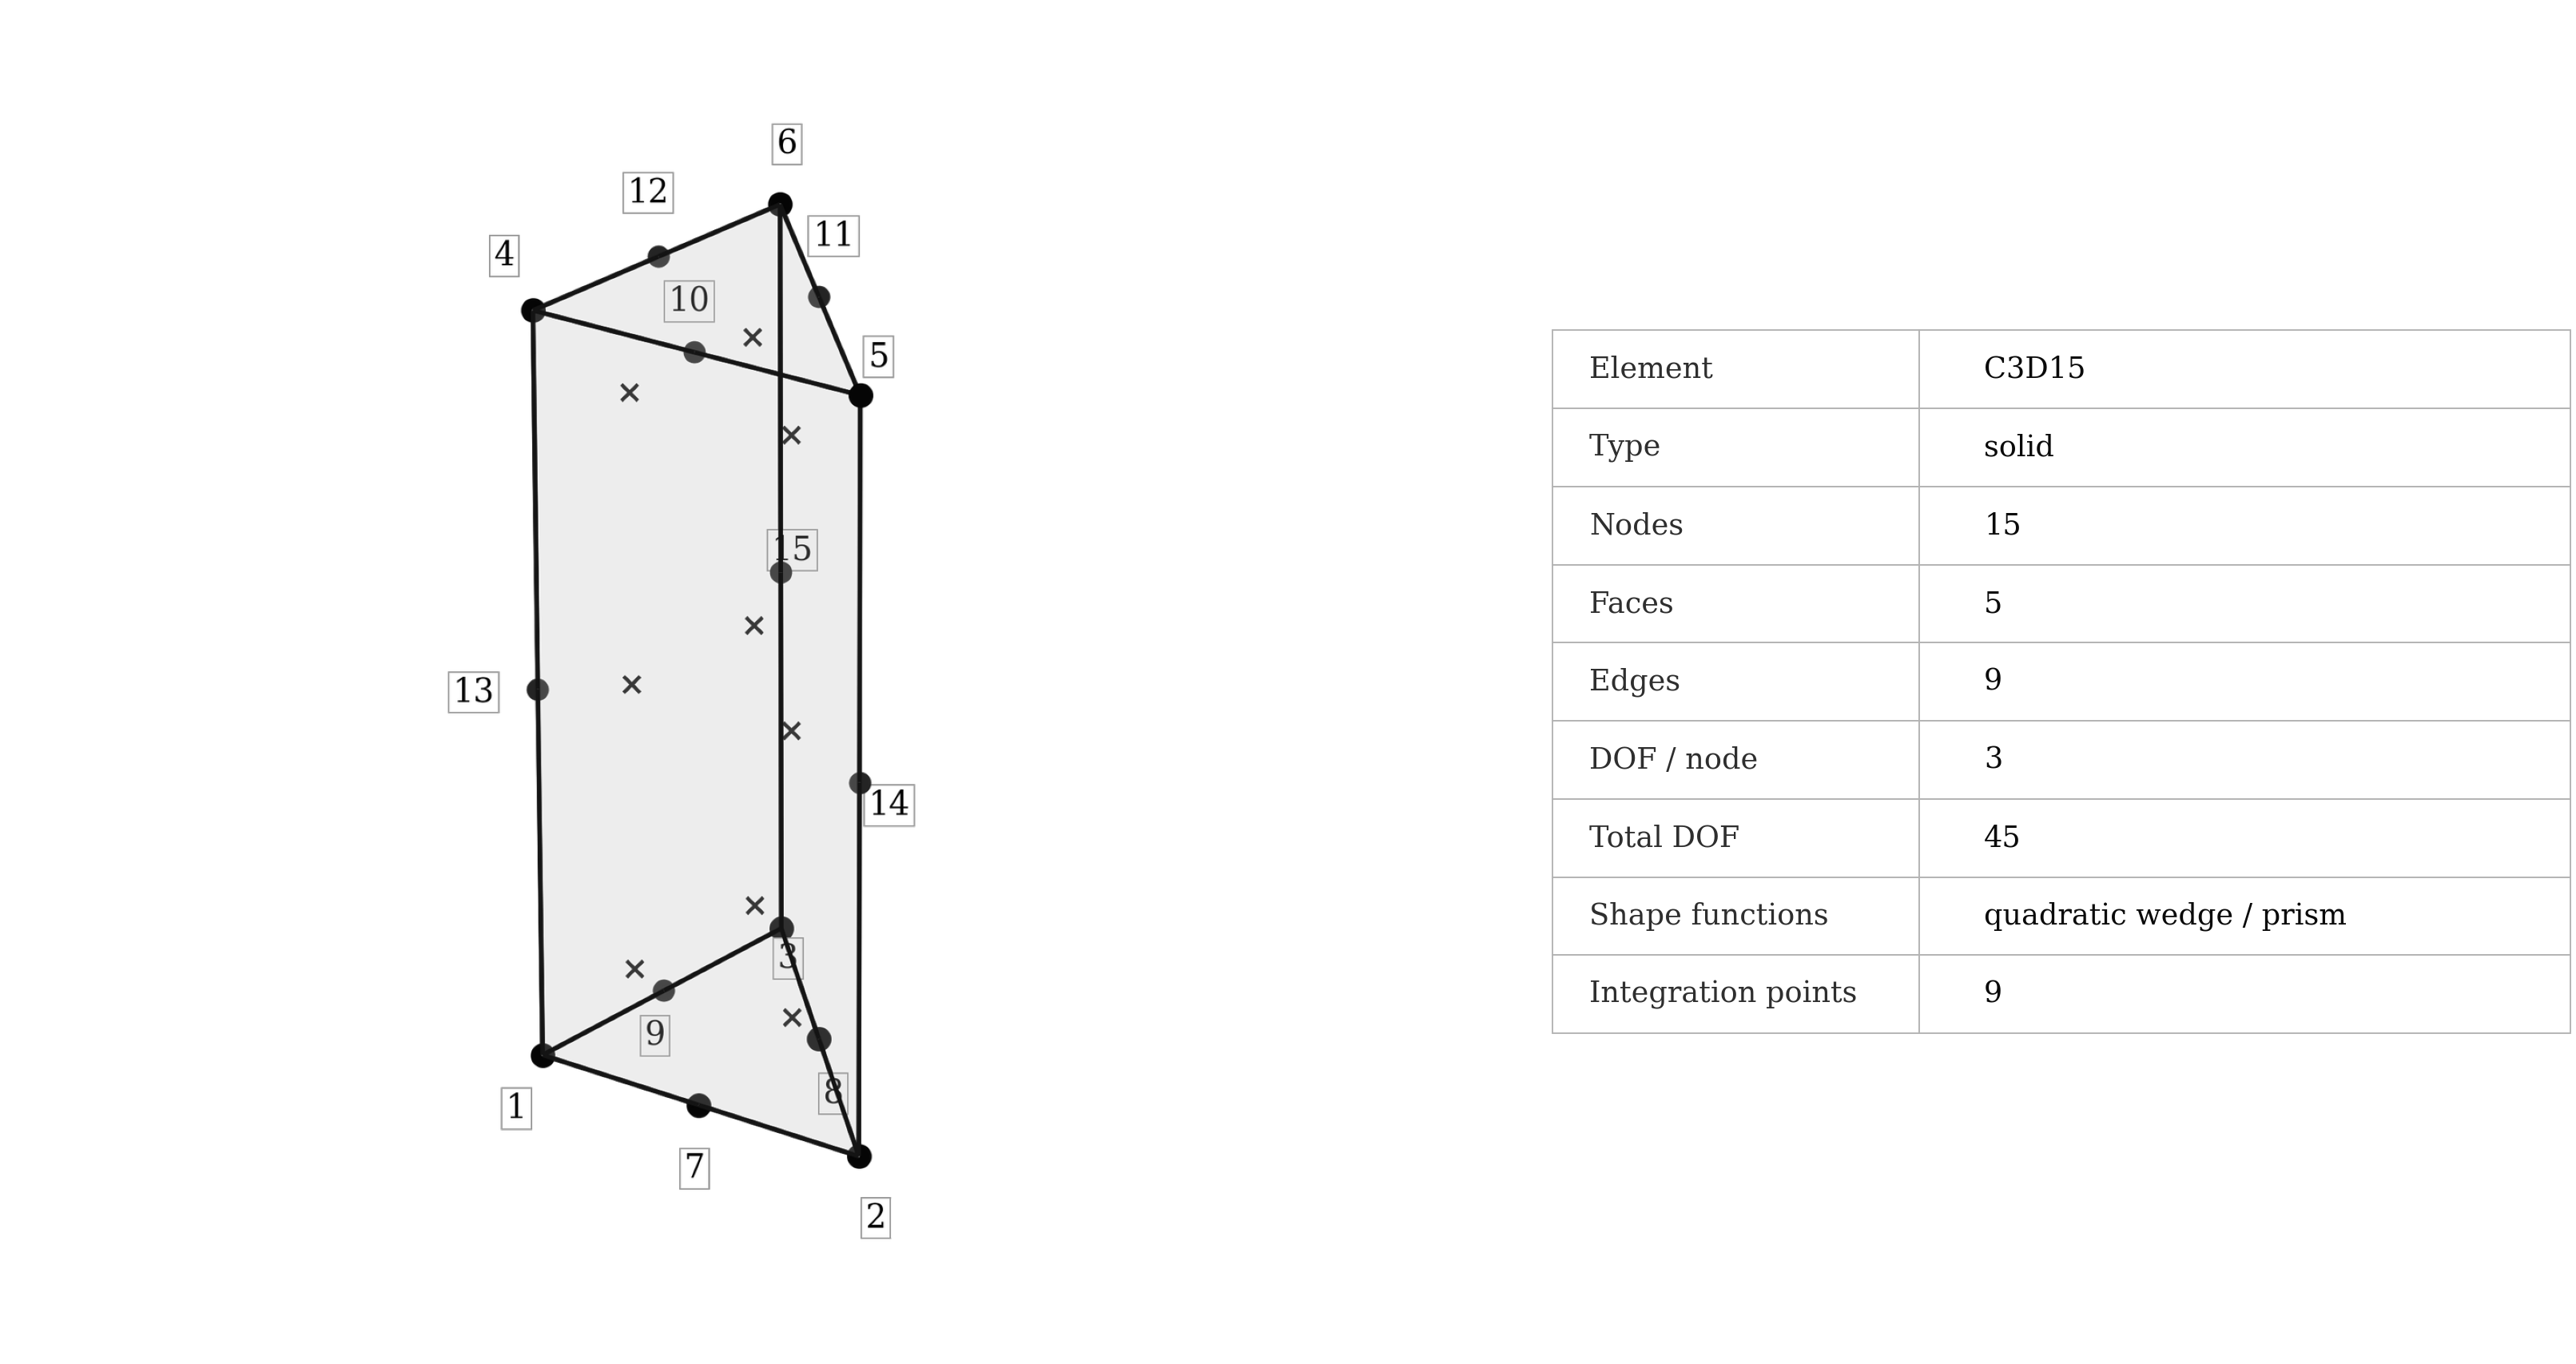
\includegraphics[width=0.80\linewidth]{pages/figures/element_schematics/c3d15_schematic.png}
    \caption{\val{C3D15} quadratic wedge element.}
\end{figure}

\begin{syntax}
*ELEMENT, TYPE=C3D15, ELSET=<set>
<id>, <n1>, ..., <n15>
\end{syntax}

\val{C3D15} is the quadratic counterpart of the six-node wedge. It adds midside nodes and represents curvature, bending, and through-thickness gradients at higher order than \val{C3D6}. Its topology matches higher-order swept meshes and prismatic regions created by extruding a quadratic triangular surface mesh.

The element combines wedge topology with higher-order through-thickness interpolation. Curved swept solids, local layered regions, and transition zones can therefore require fewer elements than with \val{C3D6}.

Higher-order mapping increases sensitivity to midside-node placement. Poorly shaped triangular end faces, excessive twisting of the side faces, and midside nodes that depart from the intended geometry degrade the mapping. A high-order wedge with a poor mapping is not automatically more accurate than a clean low-order mesh.

\val{C3D15} represents quadratic wedge meshes. A structured quadratic hexahedral mesh provides the more regular \val{C3D20} topology where geometry permits it, whereas \val{C3D10} supports fully unstructured complex geometry.

\clearpage
\paragraph{\val{C3D20}: 20-node quadratic hexahedral solid}

\begin{figure}[H]
    \centering
    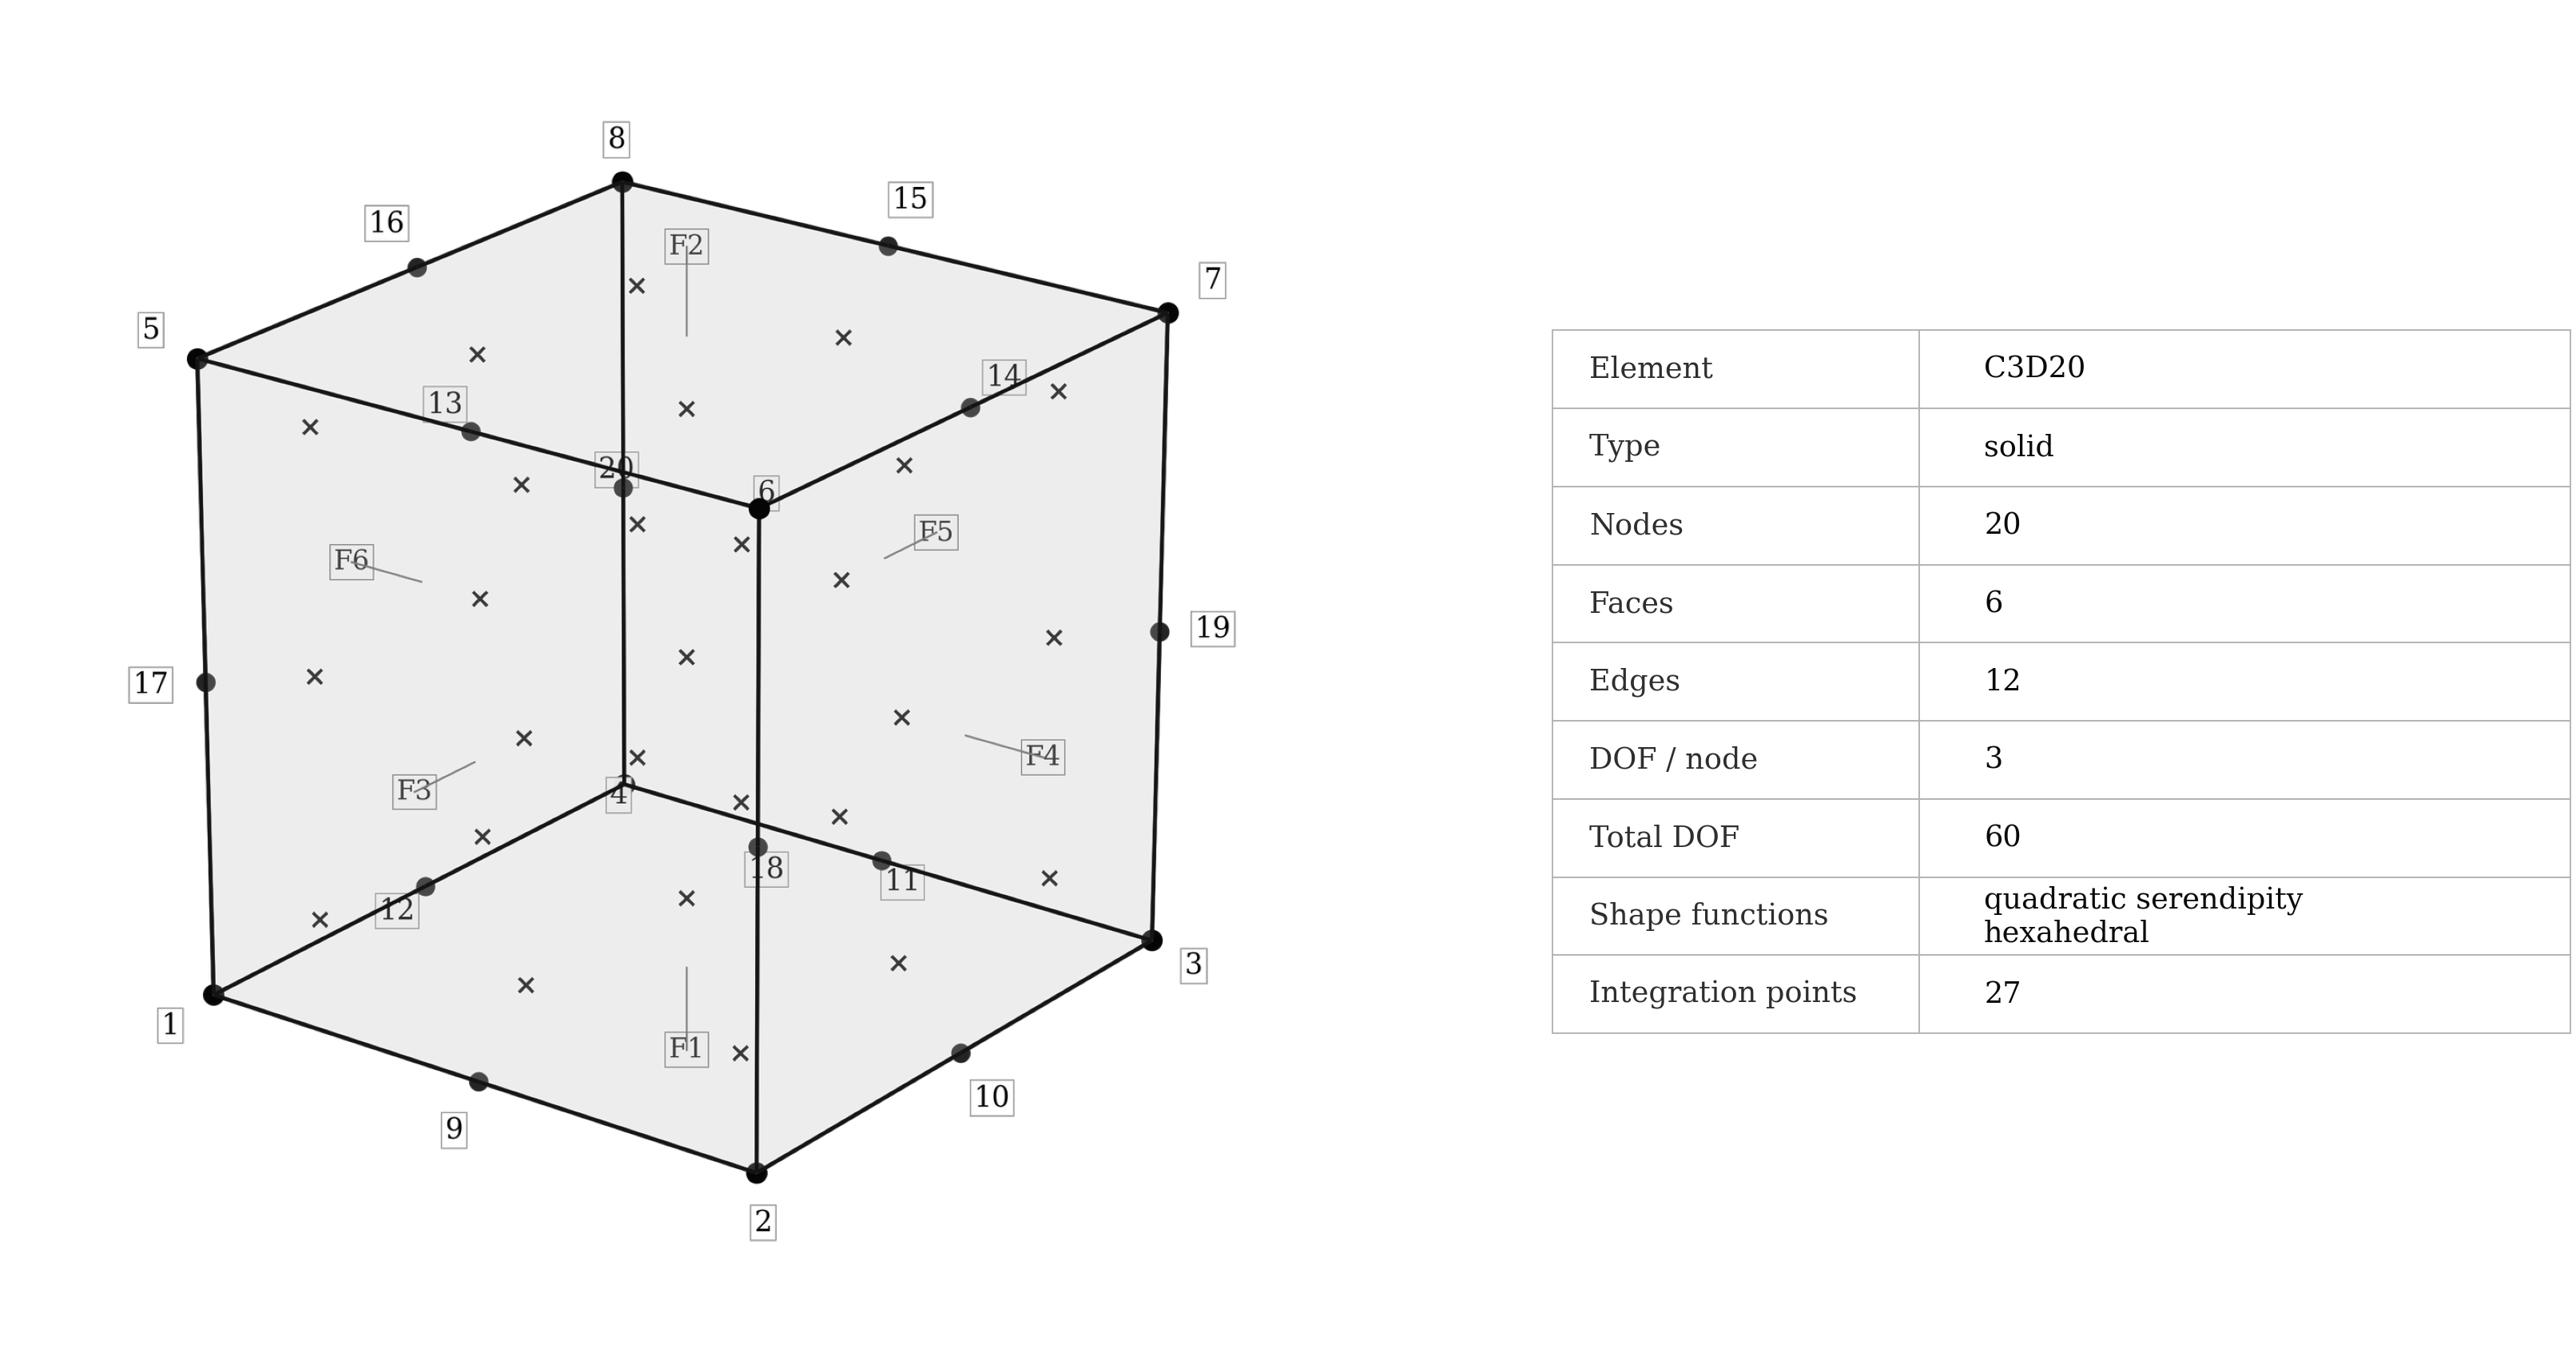
\includegraphics[width=0.82\linewidth]{pages/figures/element_schematics/c3d20_schematic.png}
    \caption{\val{C3D20} quadratic hexahedral element.}
\end{figure}

\begin{syntax}
*ELEMENT, TYPE=C3D20, ELSET=<set>
<id>, <n1>, ..., <n20>
\end{syntax}

\val{C3D20} is the full-integration quadratic hexahedral solid. The eight corner nodes are supplemented by twelve midside nodes, giving the element higher-order bending and stress-gradient representation than \val{C3D8}. Curved geometry is also represented at higher order when midside nodes follow the physical boundary.

For smooth structural fields and high-quality structured meshes, \val{C3D20} provides high-order solid accuracy. Its quadratic hexahedral interpolation represents curved blocks, swept volumes, thick structural regions, and smooth stress gradients.

The main costs are larger element matrices and stricter geometric quality requirements. Distortion of a quadratic mapping can be more harmful than distortion of a linear one because the midside nodes participate directly in the geometry interpolation. Jacobian quality therefore depends on both corner and midside-node positions.

Relative to \val{C3D8}, \val{C3D20} exchanges larger element matrices for higher-order accuracy. A fine regular \val{C3D8} mesh can remain less expensive for models dominated by linear global stiffness.

\clearpage
\paragraph{\val{C3D20R}: 20-node reduced-integration hexahedral solid}

\begin{figure}[H]
    \centering
    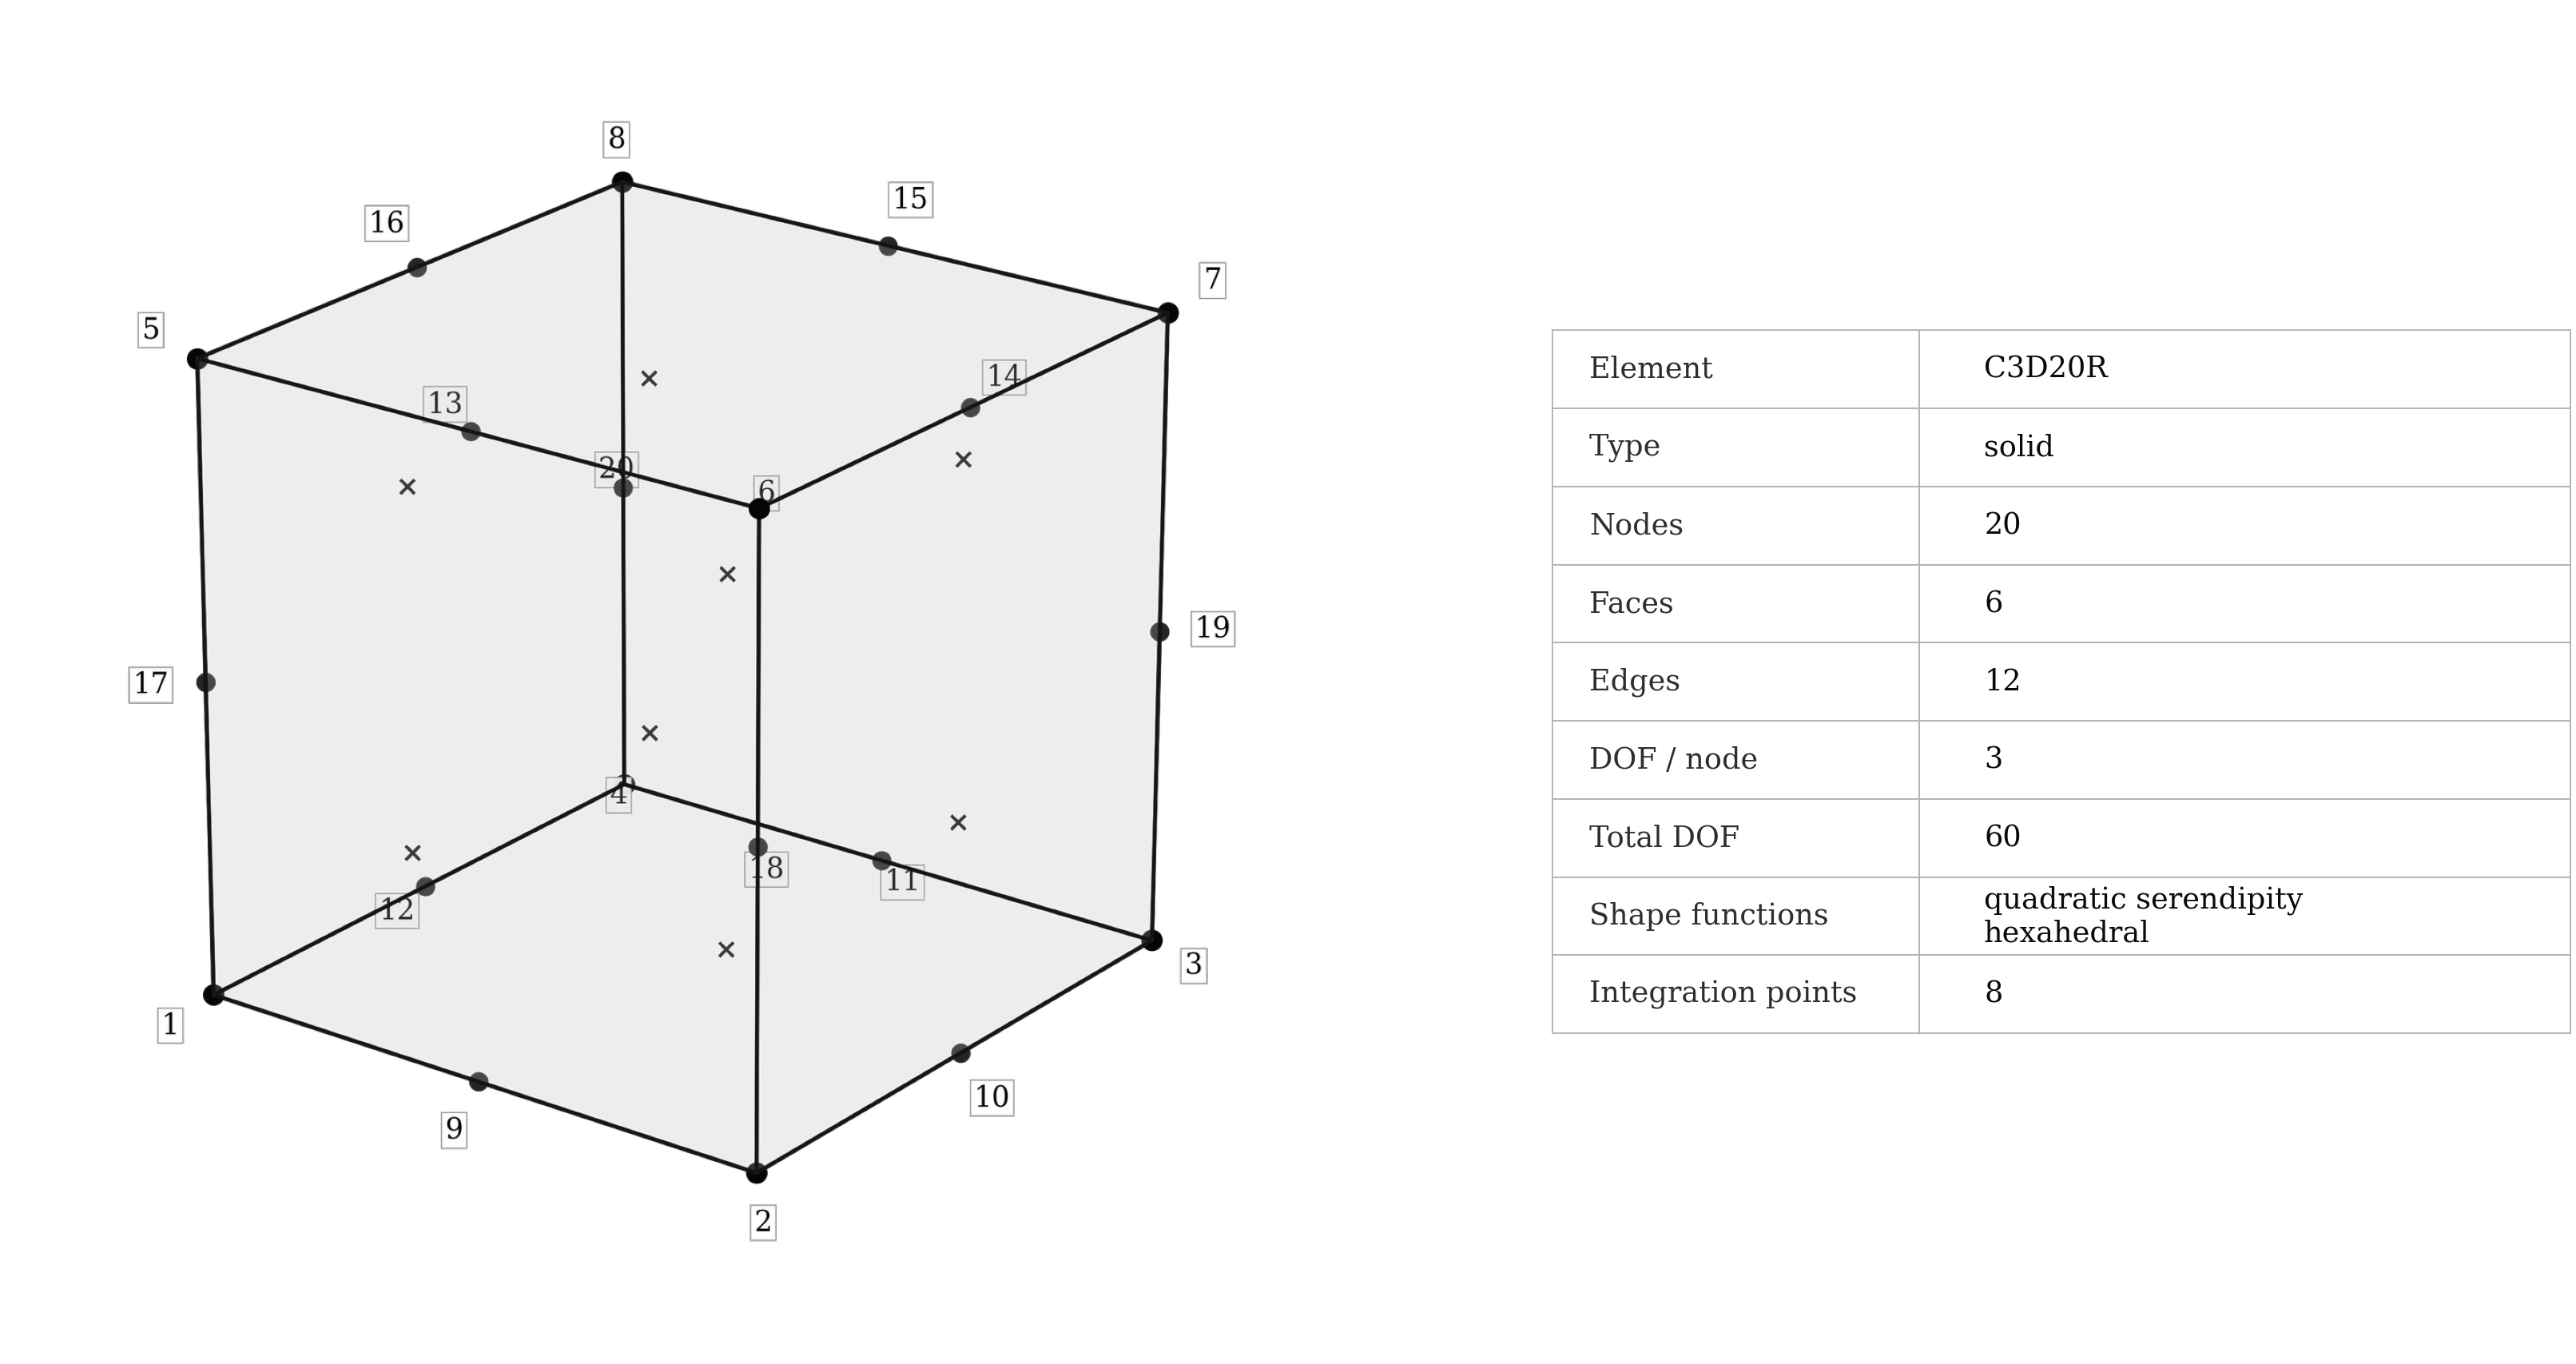
\includegraphics[width=0.82\linewidth]{pages/figures/element_schematics/c3d20r_schematic.png}
    \caption{\val{C3D20R} reduced-integration quadratic hexahedral solid element.}
\end{figure}

\begin{syntax}
*ELEMENT, TYPE=C3D20R, ELSET=<set>
<id>, <n1>, ..., <n20>
\end{syntax}

\val{C3D20R} uses the same twenty-node topology and quadratic interpolation as \val{C3D20}, but the stiffness contribution is evaluated with reduced integration. The reduced rule lowers cost and can improve behaviour in states where full integration introduces excessive constraint or stiffness.

Reduced integration changes the numerical character of the element; it is not merely a faster switch. Nonphysical low-energy deformation modes and sensitivity to mesh distortion can appear in deformed shapes, reaction balance, strain-energy distribution, and comparison with \val{C3D20}.

The formulation combines a quadratic hexahedral mesh with reduced integration. \val{C3D20} provides the corresponding fully integrated comparison formulation.

Solid stress and strain recovery is performed at the constitutive integration points and then extrapolated to element nodes; global nodal results are averaged over element contributions. An element with fewer integration points cannot provide the same recovered spatial variation as its full-integration counterpart. See Section~\ref{sec:output-results} for the distinction between integration-point, element-nodal, and averaged nodal fields.

\clearpage
\subsubsection{Shell elements}

Shell elements model thin-walled structures through a two-dimensional
reference surface with an assigned thickness or generalized sectional
stiffness. Their kinematics represent membrane stretching, bending,
and transverse shear without discretizing the thickness with
continuum elements. FEMaster's finite-rotation shells use independent
nodal translations and rotations, so the current orientation of
the shell can be represented directly. Typical applications include
plates, aircraft skins, curved panels, and other lightweight
structures dominated by midsurface deformation.

The recovered quantities include membrane forces, bending moments,
transverse-shear resultants, and supported top/bottom stresses, but
not an arbitrary three-dimensional through-thickness stress field.
A solid model may be more suitable near concentrated load
introductions, connections, or locations with significant thickness
effects. The shell normal determines the top/bottom convention,
affects pressure direction, and enters the interpretation of bending
results. Mesh quality, surface orientation, thickness, and material
directions must therefore be defined consistently.

Four finite-rotation formulations are available, covering triangular
and quadrilateral topologies with linear and quadratic geometric
interpolation. Triangular meshes accommodate irregular boundaries,
while quadrilateral meshes are particularly effective on structured
surfaces. Higher-order elements resolve smooth curvature more
efficiently but increase element cost and require well-positioned
midside nodes. Each heading lists all accepted aliases of the same
FEMaster implementation.

\clearpage
\paragraph{\val{MITC3FRT} / \val{S3} / \val{S3R}: 3-node finite-rotation triangular shell}

\begin{figure}[H]
    \centering
    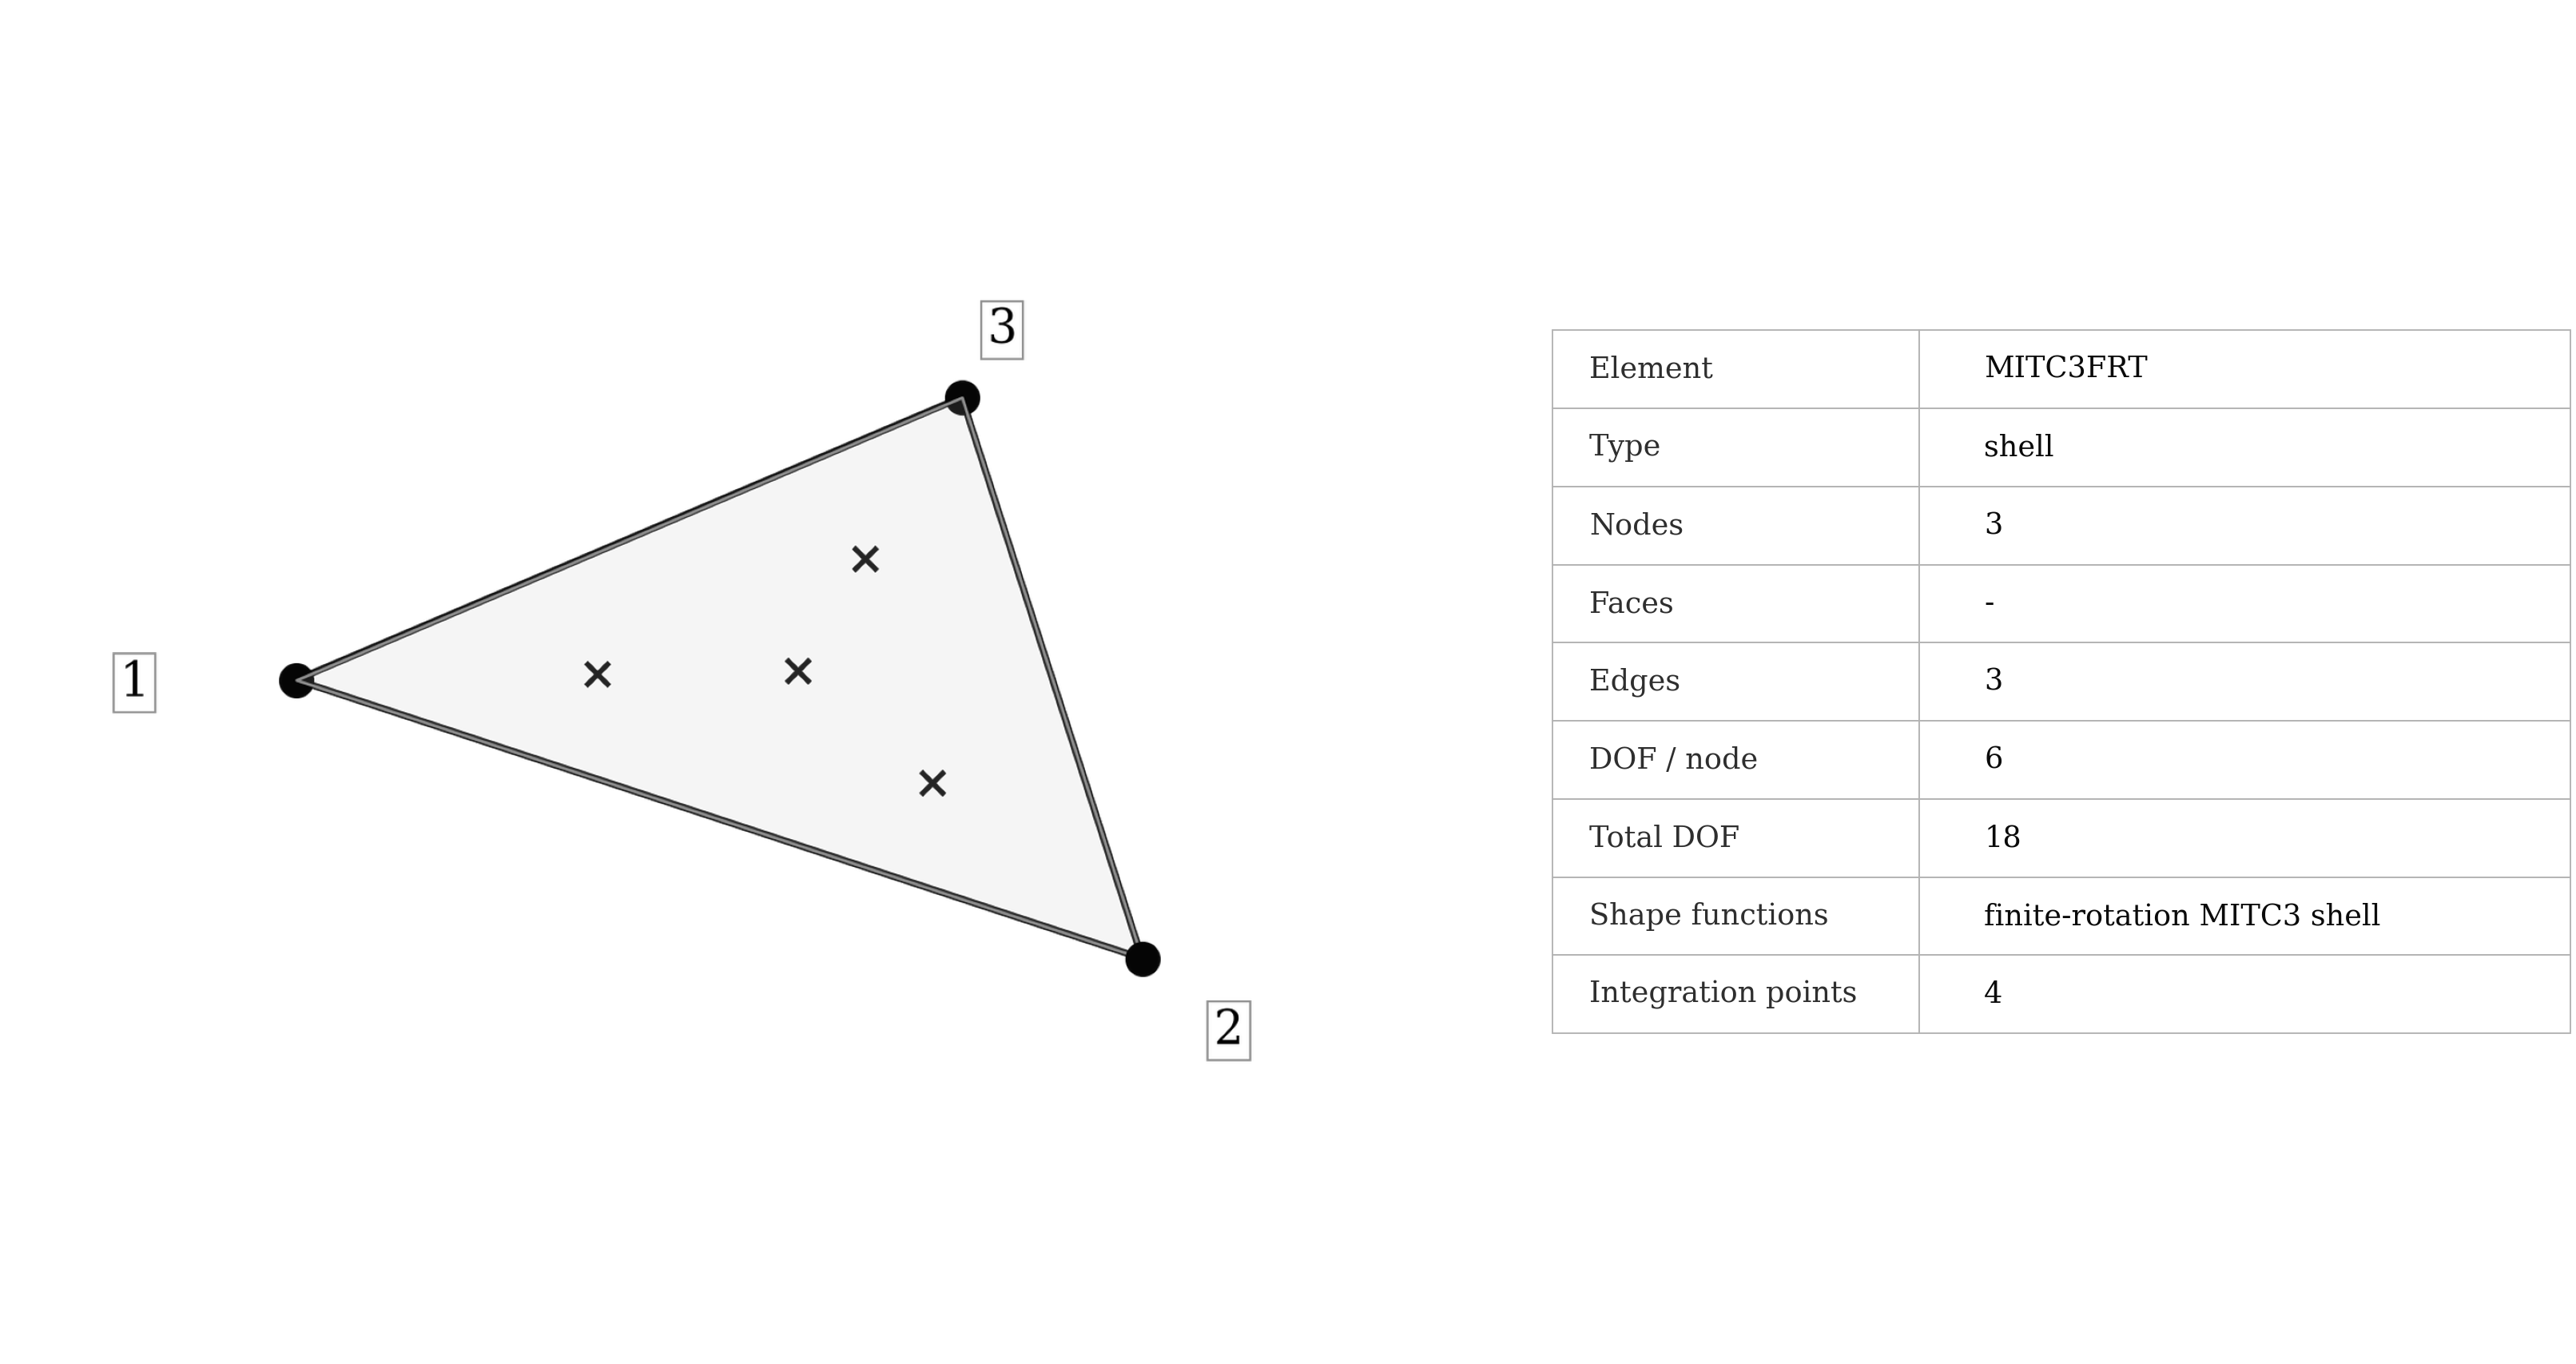
\includegraphics[width=0.76\linewidth]{pages/figures/element_schematics/mitc3frt_schematic.png}
    \caption{Three-node finite-rotation triangular shell geometry and node ordering.}
\end{figure}

\begin{syntax}
*ELEMENT, TYPE=MITC3FRT, ELSET=<set>
<id>, <n1>, <n2>, <n3>
\end{syntax}

The three-node triangular shell combines a linear geometric
interpolation with finite-rotation kinematics and independent nodal
translations and rotations. It represents membrane deformation,
bending, and transverse shear within the common shell framework.
This compact topology is useful for unstructured surface meshes,
irregular boundaries, openings, and transitions where a regular
quadrilateral mesh would be difficult to construct.

A single linear triangle has limited resolution of curved geometry
and spatially varying bending fields. Bending-dominated or strongly
curved models therefore require refinement, with convergence checked
using displacements, stresses or shell resultants, and strain energy.
The aliases \val{S3} and \val{S3R} select the same implementation as
\val{MITC3FRT}; the \val{R} suffix does not select a separate
reduced-integration formulation in FEMaster.

\clearpage
\paragraph{\val{MITC4FRT} / \val{S4} / \val{S4R} / \val{MITC4}: 4-node finite-rotation quadrilateral shell}

\begin{figure}[H]
    \centering
    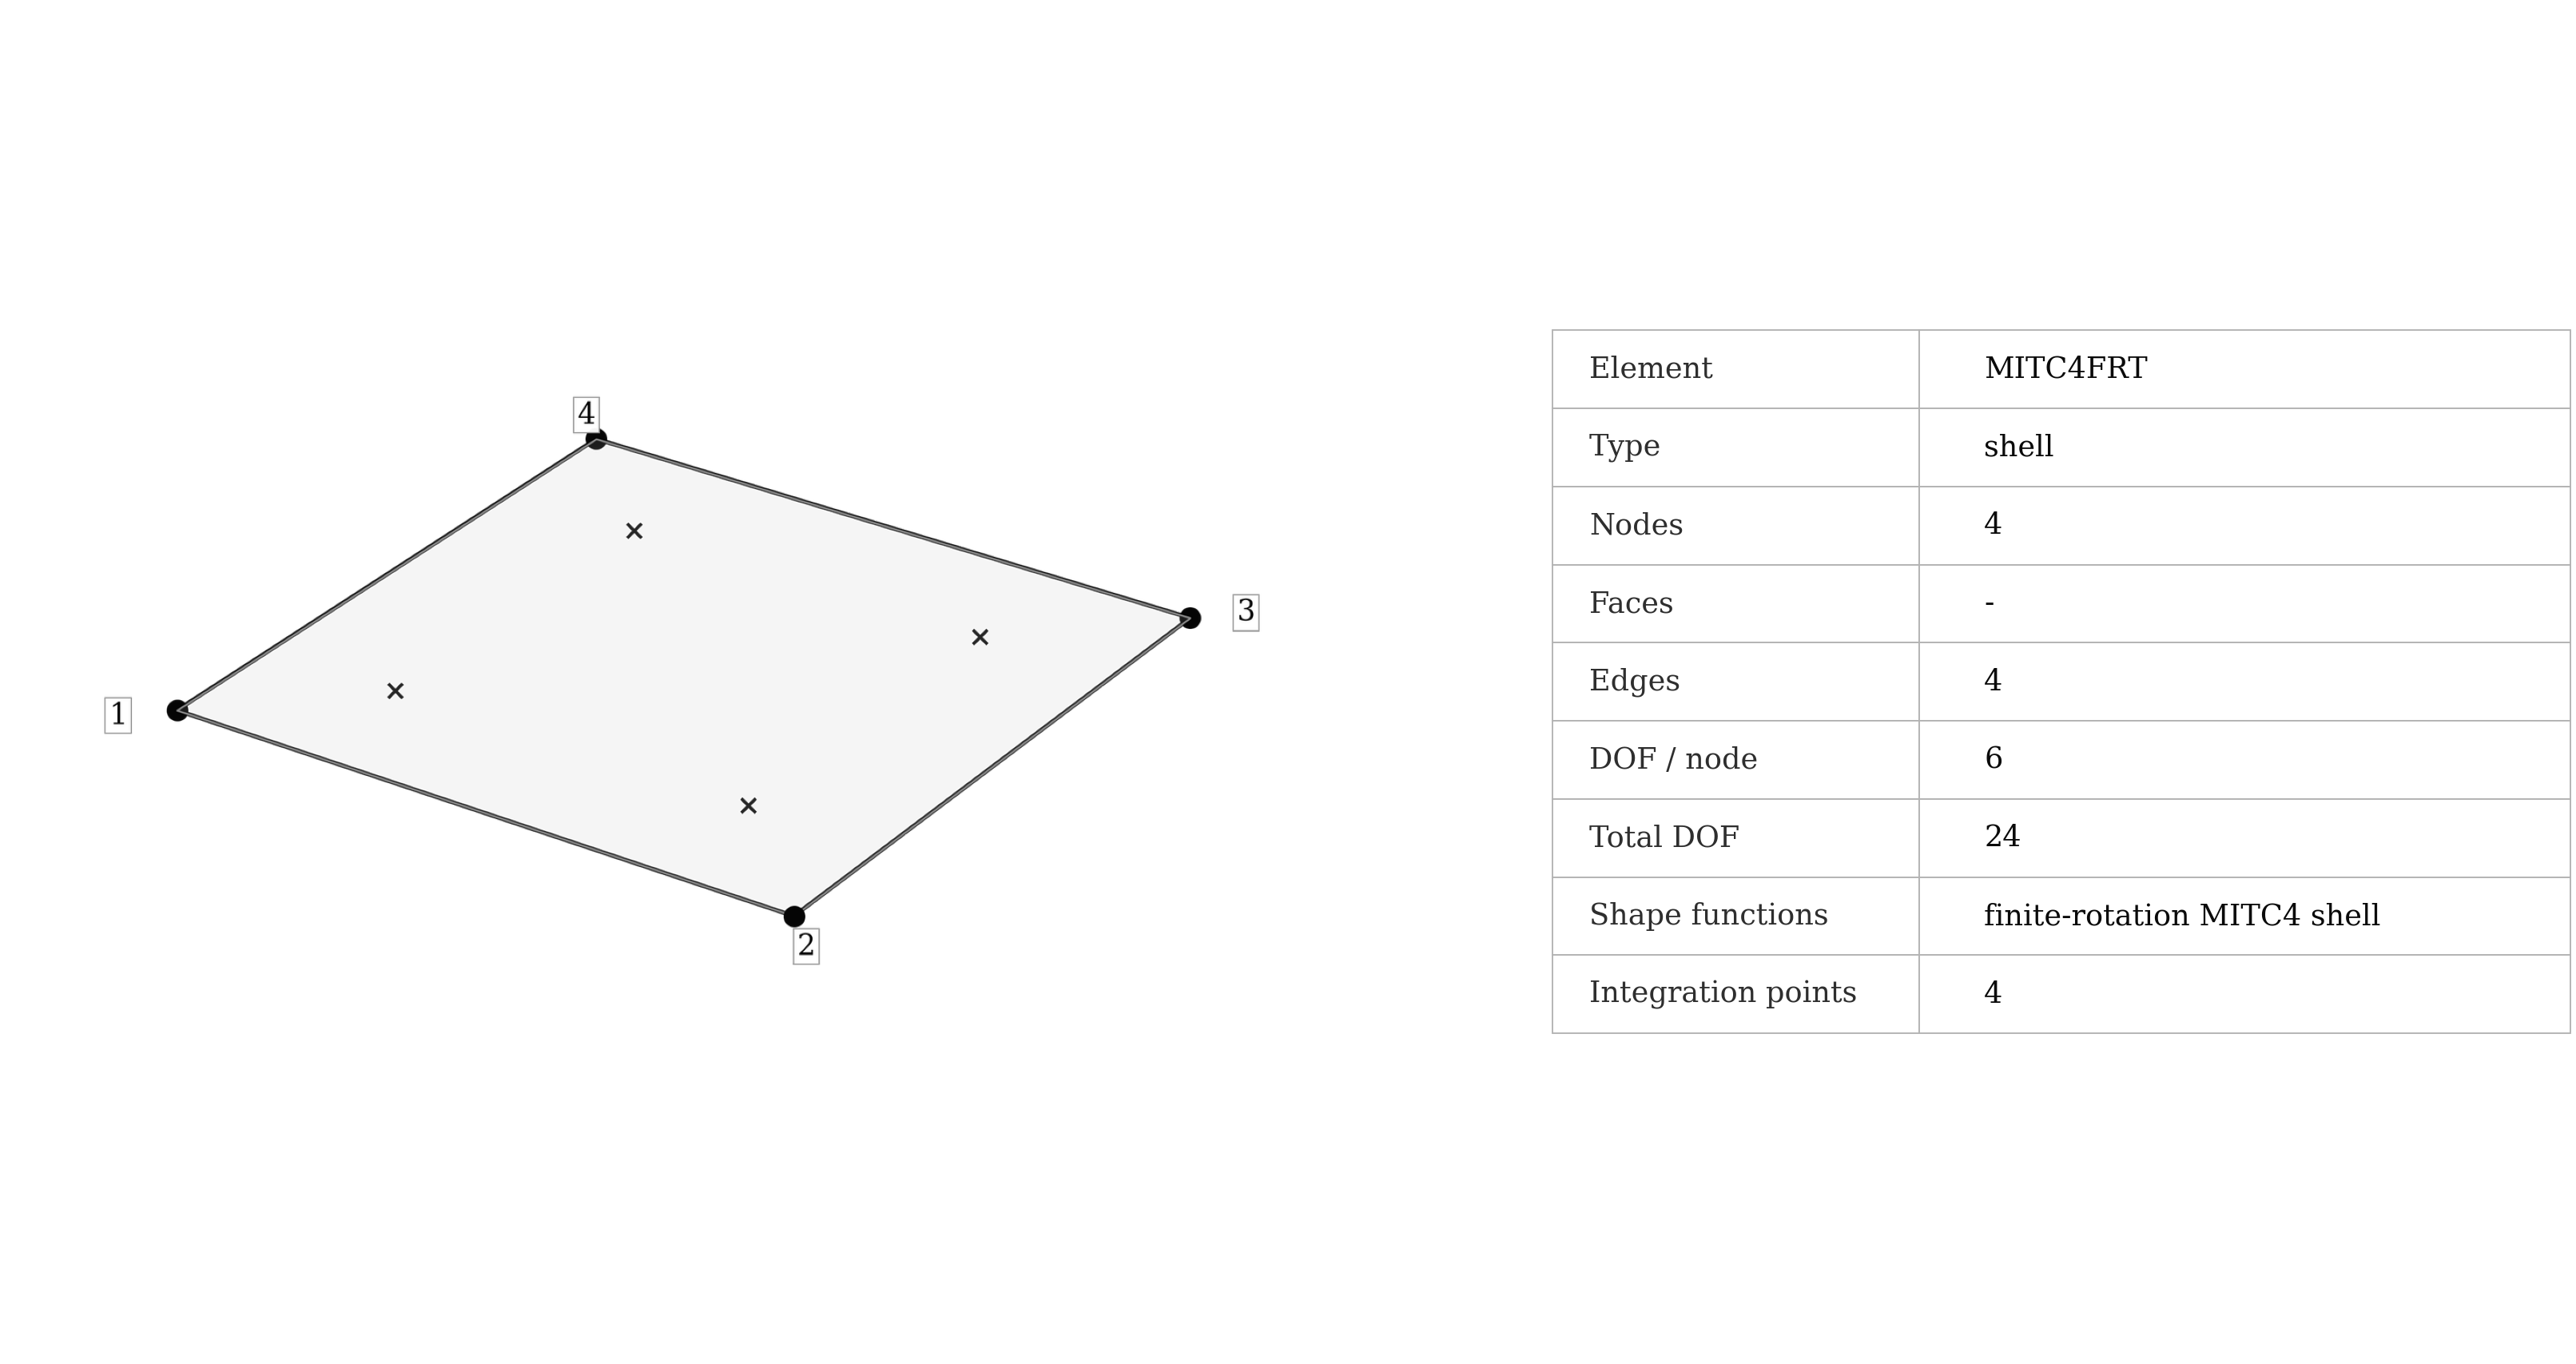
\includegraphics[width=0.78\linewidth]{pages/figures/element_schematics/mitc4frt_schematic.png}
    \caption{Four-node finite-rotation MITC shell geometry and node ordering.}
\end{figure}

\begin{syntax}
*ELEMENT, TYPE=MITC4FRT, ELSET=<set>
<id>, <n1>, <n2>, <n3>, <n4>
\end{syntax}

The four-node quadrilateral shell combines finite-rotation kinematics
with a Mixed Interpolation of Tensorial Components (MITC) treatment
of transverse shear. In thin-shell bending, an ordinary low-order
displacement interpolation can become artificially stiff because
the shear strains cannot approach their limiting values correctly.
This numerical effect, known as shear locking, is mitigated by the
MITC interpolation while transverse-shear deformation remains part
of the underlying shell model.

The formulation is well suited to plates, skins, stiffened panels,
and shell assemblies discretized with regular quadrilaterals. It
represents bending and twisting through independent nodal rotations
rather than an internally expanded solid mesh. Nevertheless, strong
warping, severe element skewness, and insufficient surface resolution
can reduce accuracy, especially for curved geometry and nonlinear
deformation paths. The names \val{S4}, \val{S4R}, and \val{MITC4}
are aliases for \val{MITC4FRT}; they do not select different
integration schemes.

\clearpage
\paragraph{\val{MITC6FRT} / \val{S6} / \val{S6R}: 6-node finite-rotation triangular shell}

\begin{figure}[H]
    \centering
    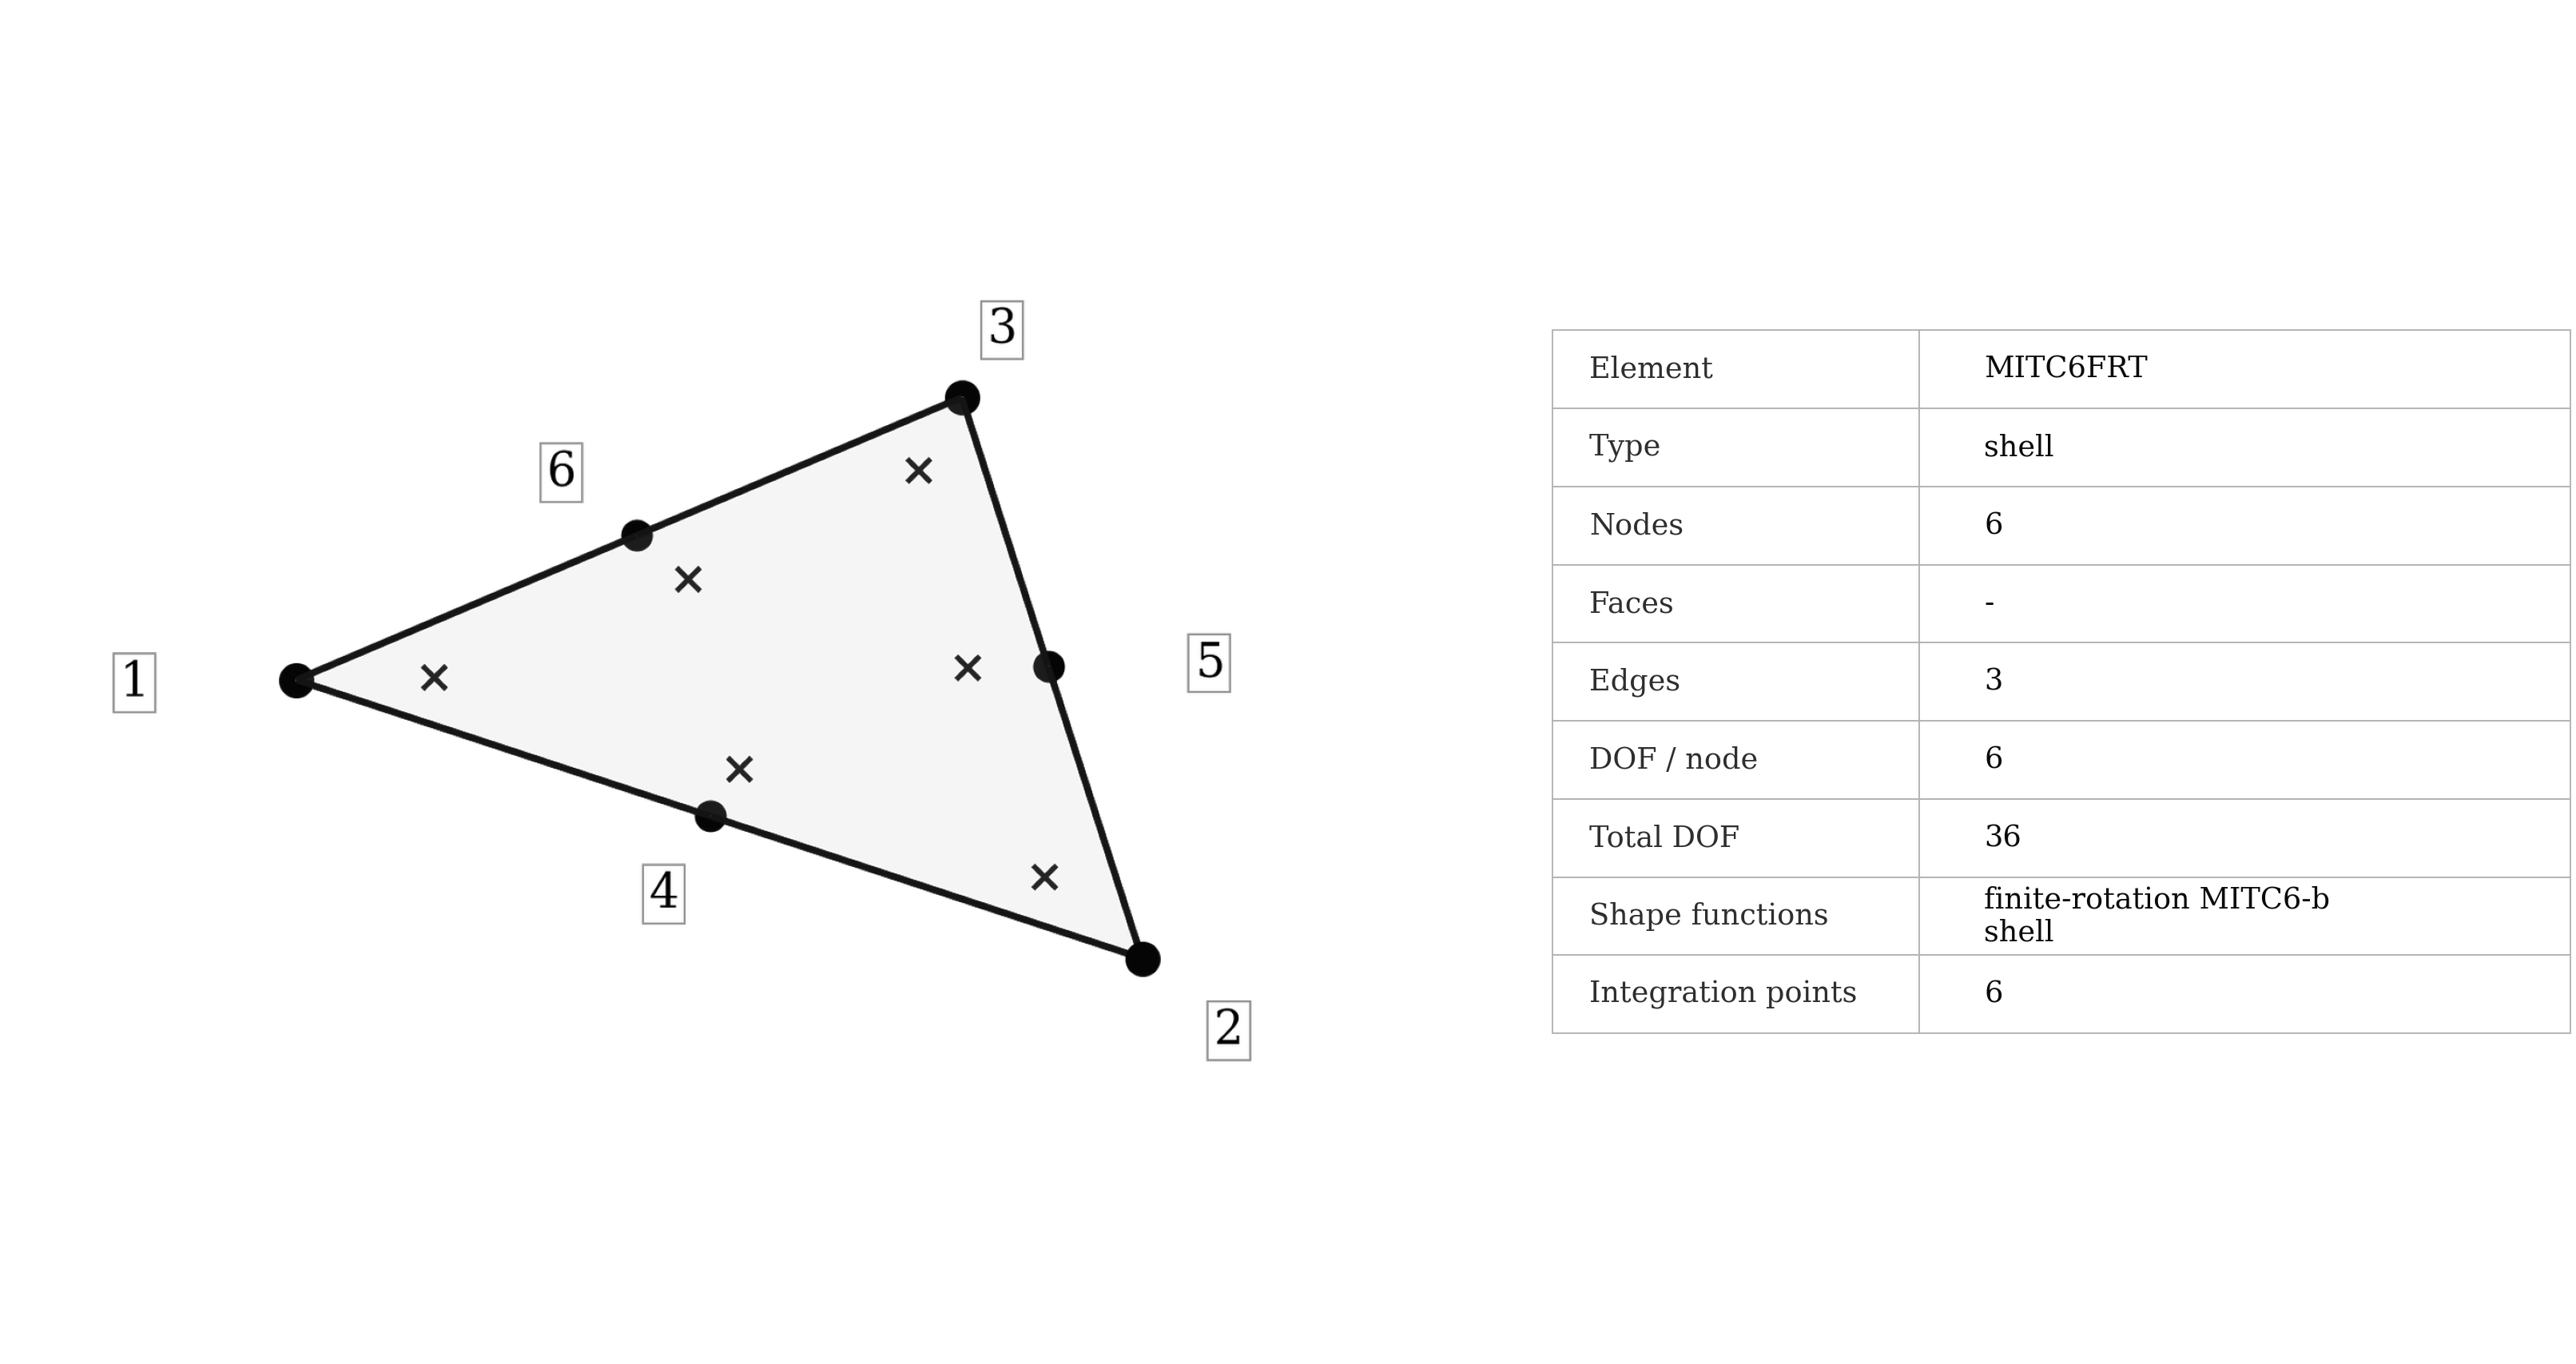
\includegraphics[width=0.78\linewidth]{pages/figures/element_schematics/mitc6frt_schematic.png}
    \caption{Six-node finite-rotation triangular shell geometry and node ordering.}
\end{figure}

\begin{syntax}
*ELEMENT, TYPE=MITC6FRT, ELSET=<set>
<id>, <n1>, <n2>, <n3>, <n4>, <n5>, <n6>
\end{syntax}

The six-node triangular shell extends the finite-rotation midsurface
description to quadratic geometric interpolation. Its midside nodes
allow curved edges and a more detailed representation of smoothly
varying displacement and bending fields than the three-node
triangle. It is useful for curved shell regions, cutouts, and
unstructured higher-order surface meshes where triangular topology
is preferred.

The higher interpolation order improves geometric flexibility but
does not eliminate sensitivity to mesh quality. Midside nodes must
follow the intended surface and highly distorted triangles can
produce inaccurate stiffness and recovered results. Thin-shell
bending calculations should therefore be checked by mesh
refinement. The \val{S6} and \val{S6R} aliases select exactly the
same FEMaster implementation as \val{MITC6FRT}.

\clearpage
\paragraph{\val{MITC8FRT} / \val{S8} / \val{S8R} / \val{MITC8}: 8-node finite-rotation quadrilateral shell}

\begin{figure}[H]
    \centering
    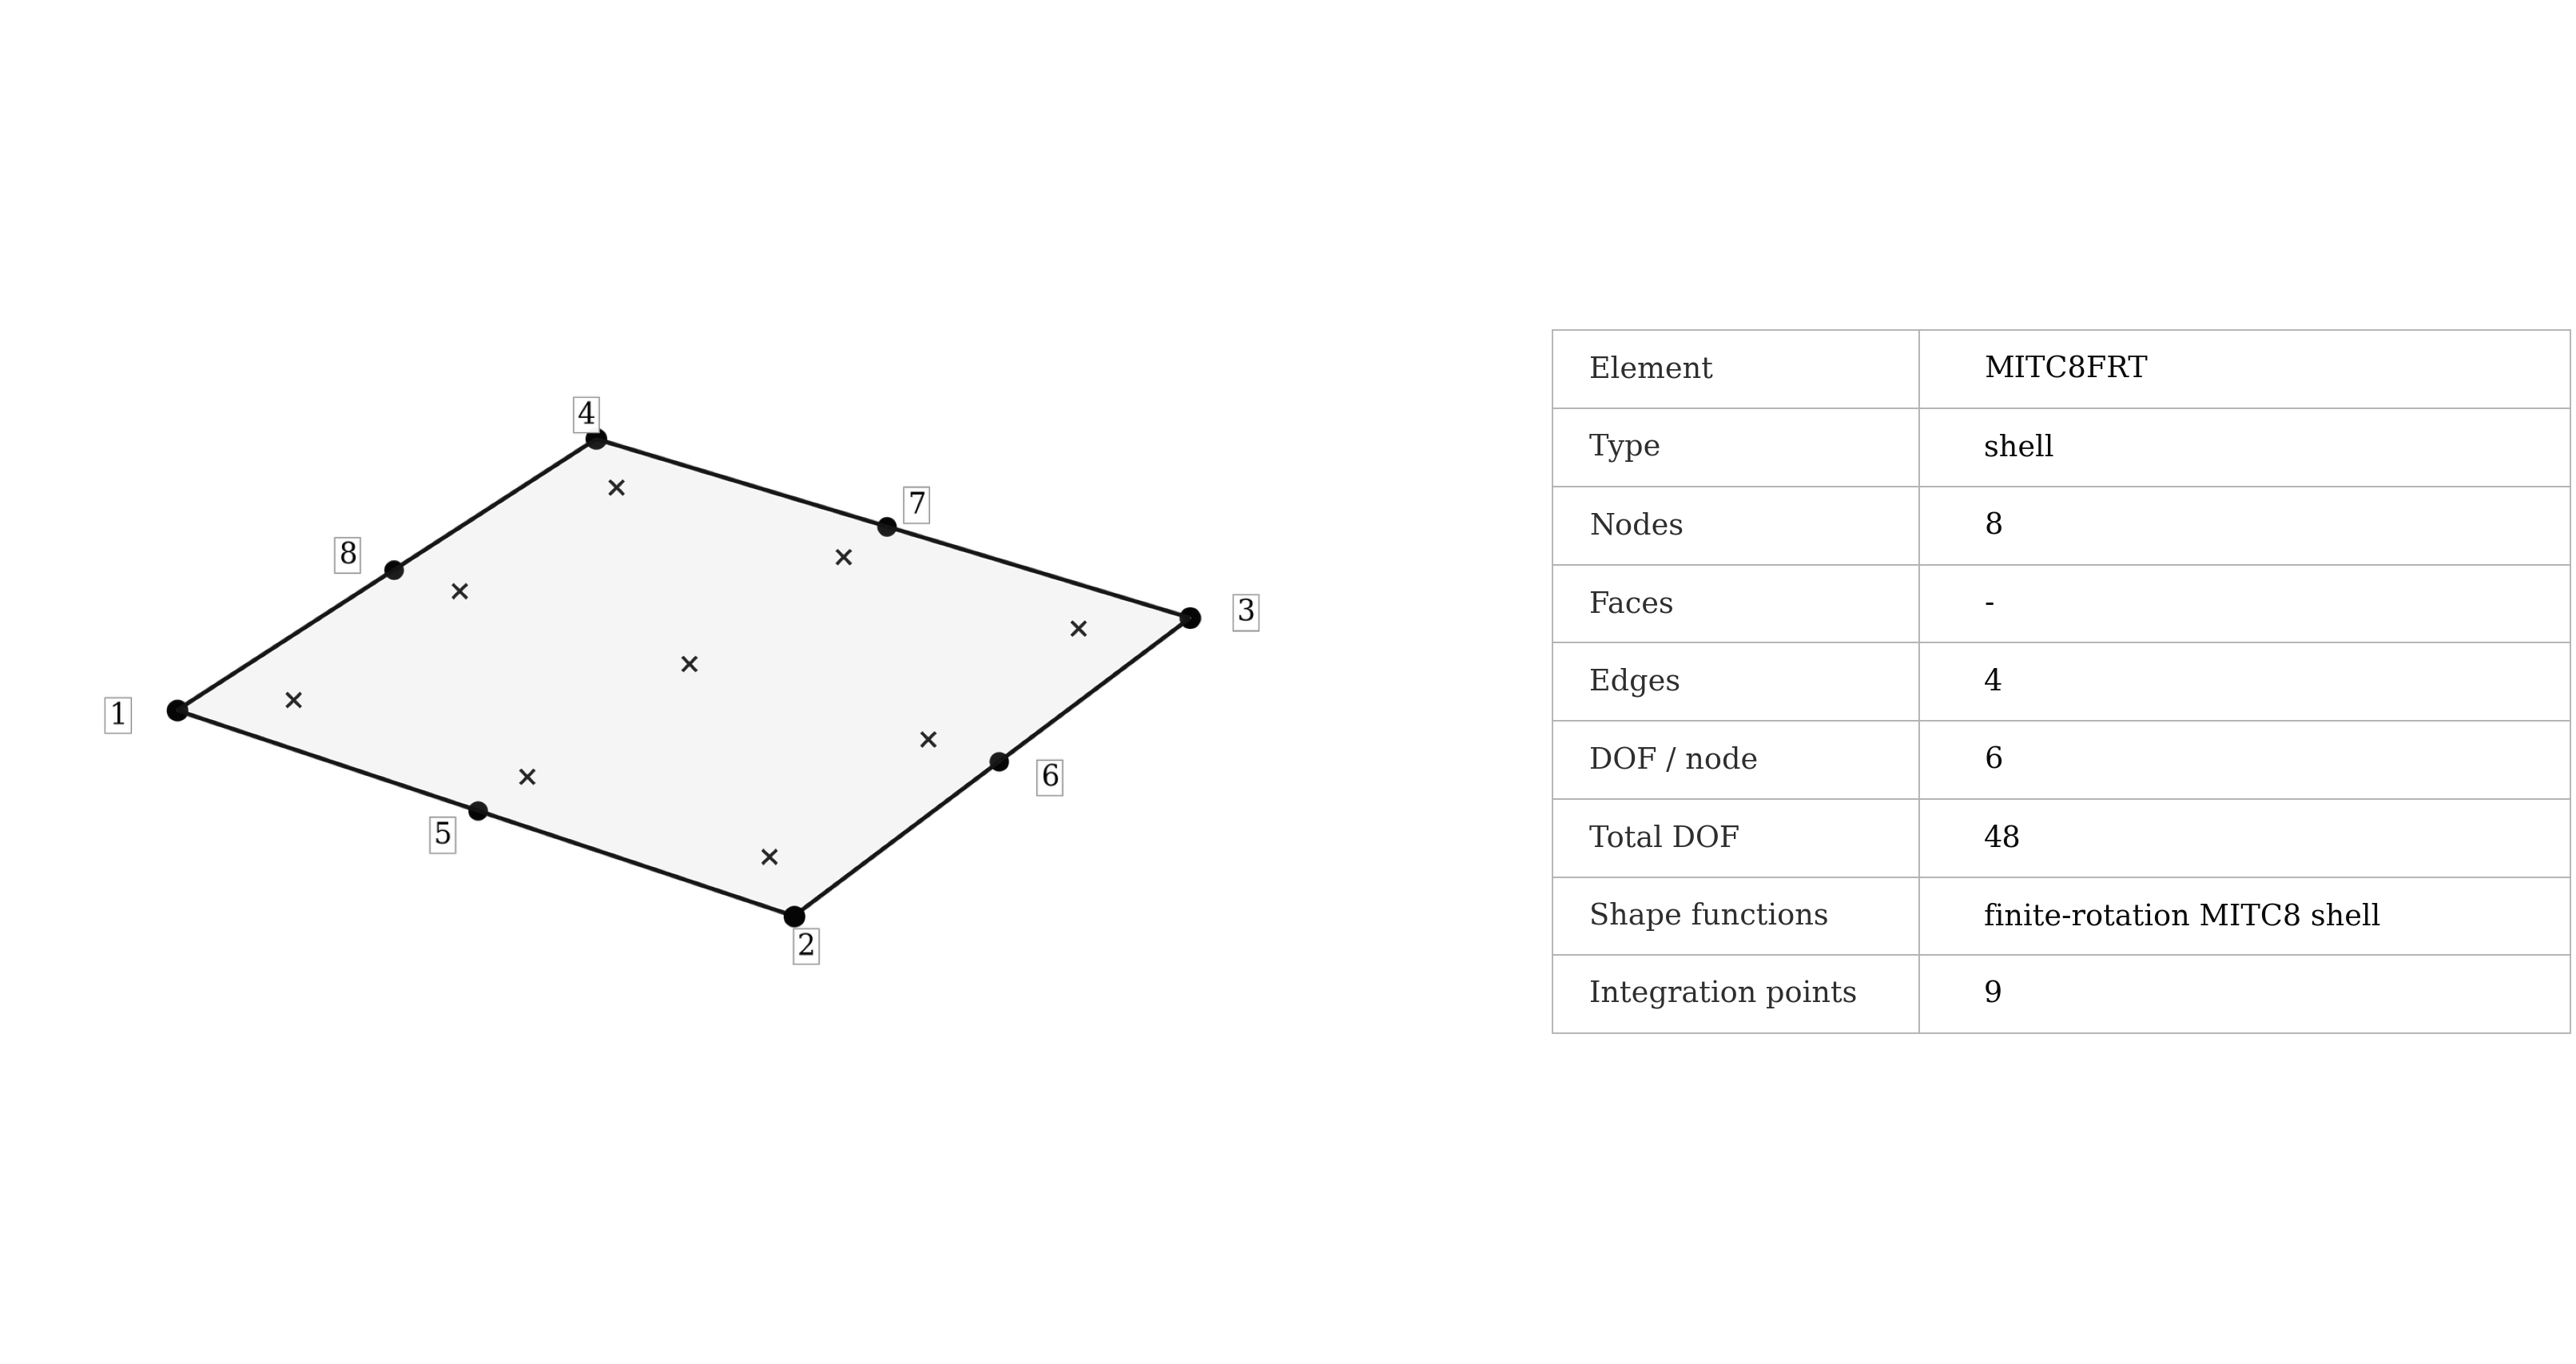
\includegraphics[width=0.80\linewidth]{pages/figures/element_schematics/mitc8frt_schematic.png}
    \caption{Eight-node finite-rotation MITC shell geometry and node ordering.}
\end{figure}

\begin{syntax}
*ELEMENT, TYPE=MITC8FRT, ELSET=<set>
<id>, <n1>, <n2>, <n3>, <n4>, <n5>, <n6>, <n7>, <n8>
\end{syntax}

The eight-node quadrilateral shell combines higher-order midsurface
interpolation, finite-rotation kinematics, and an MITC
transverse-shear treatment. The midside nodes provide a richer
description of smooth curvature, displacement, and bending fields
than the four-node element. This makes the formulation suitable
for curved panels and shell regions where accurate geometry and
smooth stress-resultant gradients are important.

Compared with \val{MITC4FRT}, the additional nodes increase
element cost but may reduce the number of elements needed for
smooth curved geometry. Accuracy still depends on the placement
of midside nodes, consistent shell normals, and acceptable element
warping. The shell idealization does not resolve detailed
through-thickness continuum stresses. The aliases \val{S8},
\val{S8R}, and \val{MITC8} select this same
\val{MITC8FRT} implementation.

Although grouped with the shell and panel formulations, \val{QSPT}
is a specialized shear-panel element rather than a general-purpose
shell. Its kinematics and recoverable quantities differ from those
of the finite-rotation MITC shells described above.

\clearpage
\paragraph{\val{QSPT}: quadrilateral shear-panel element}

\begin{figure}[H]
    \centering
    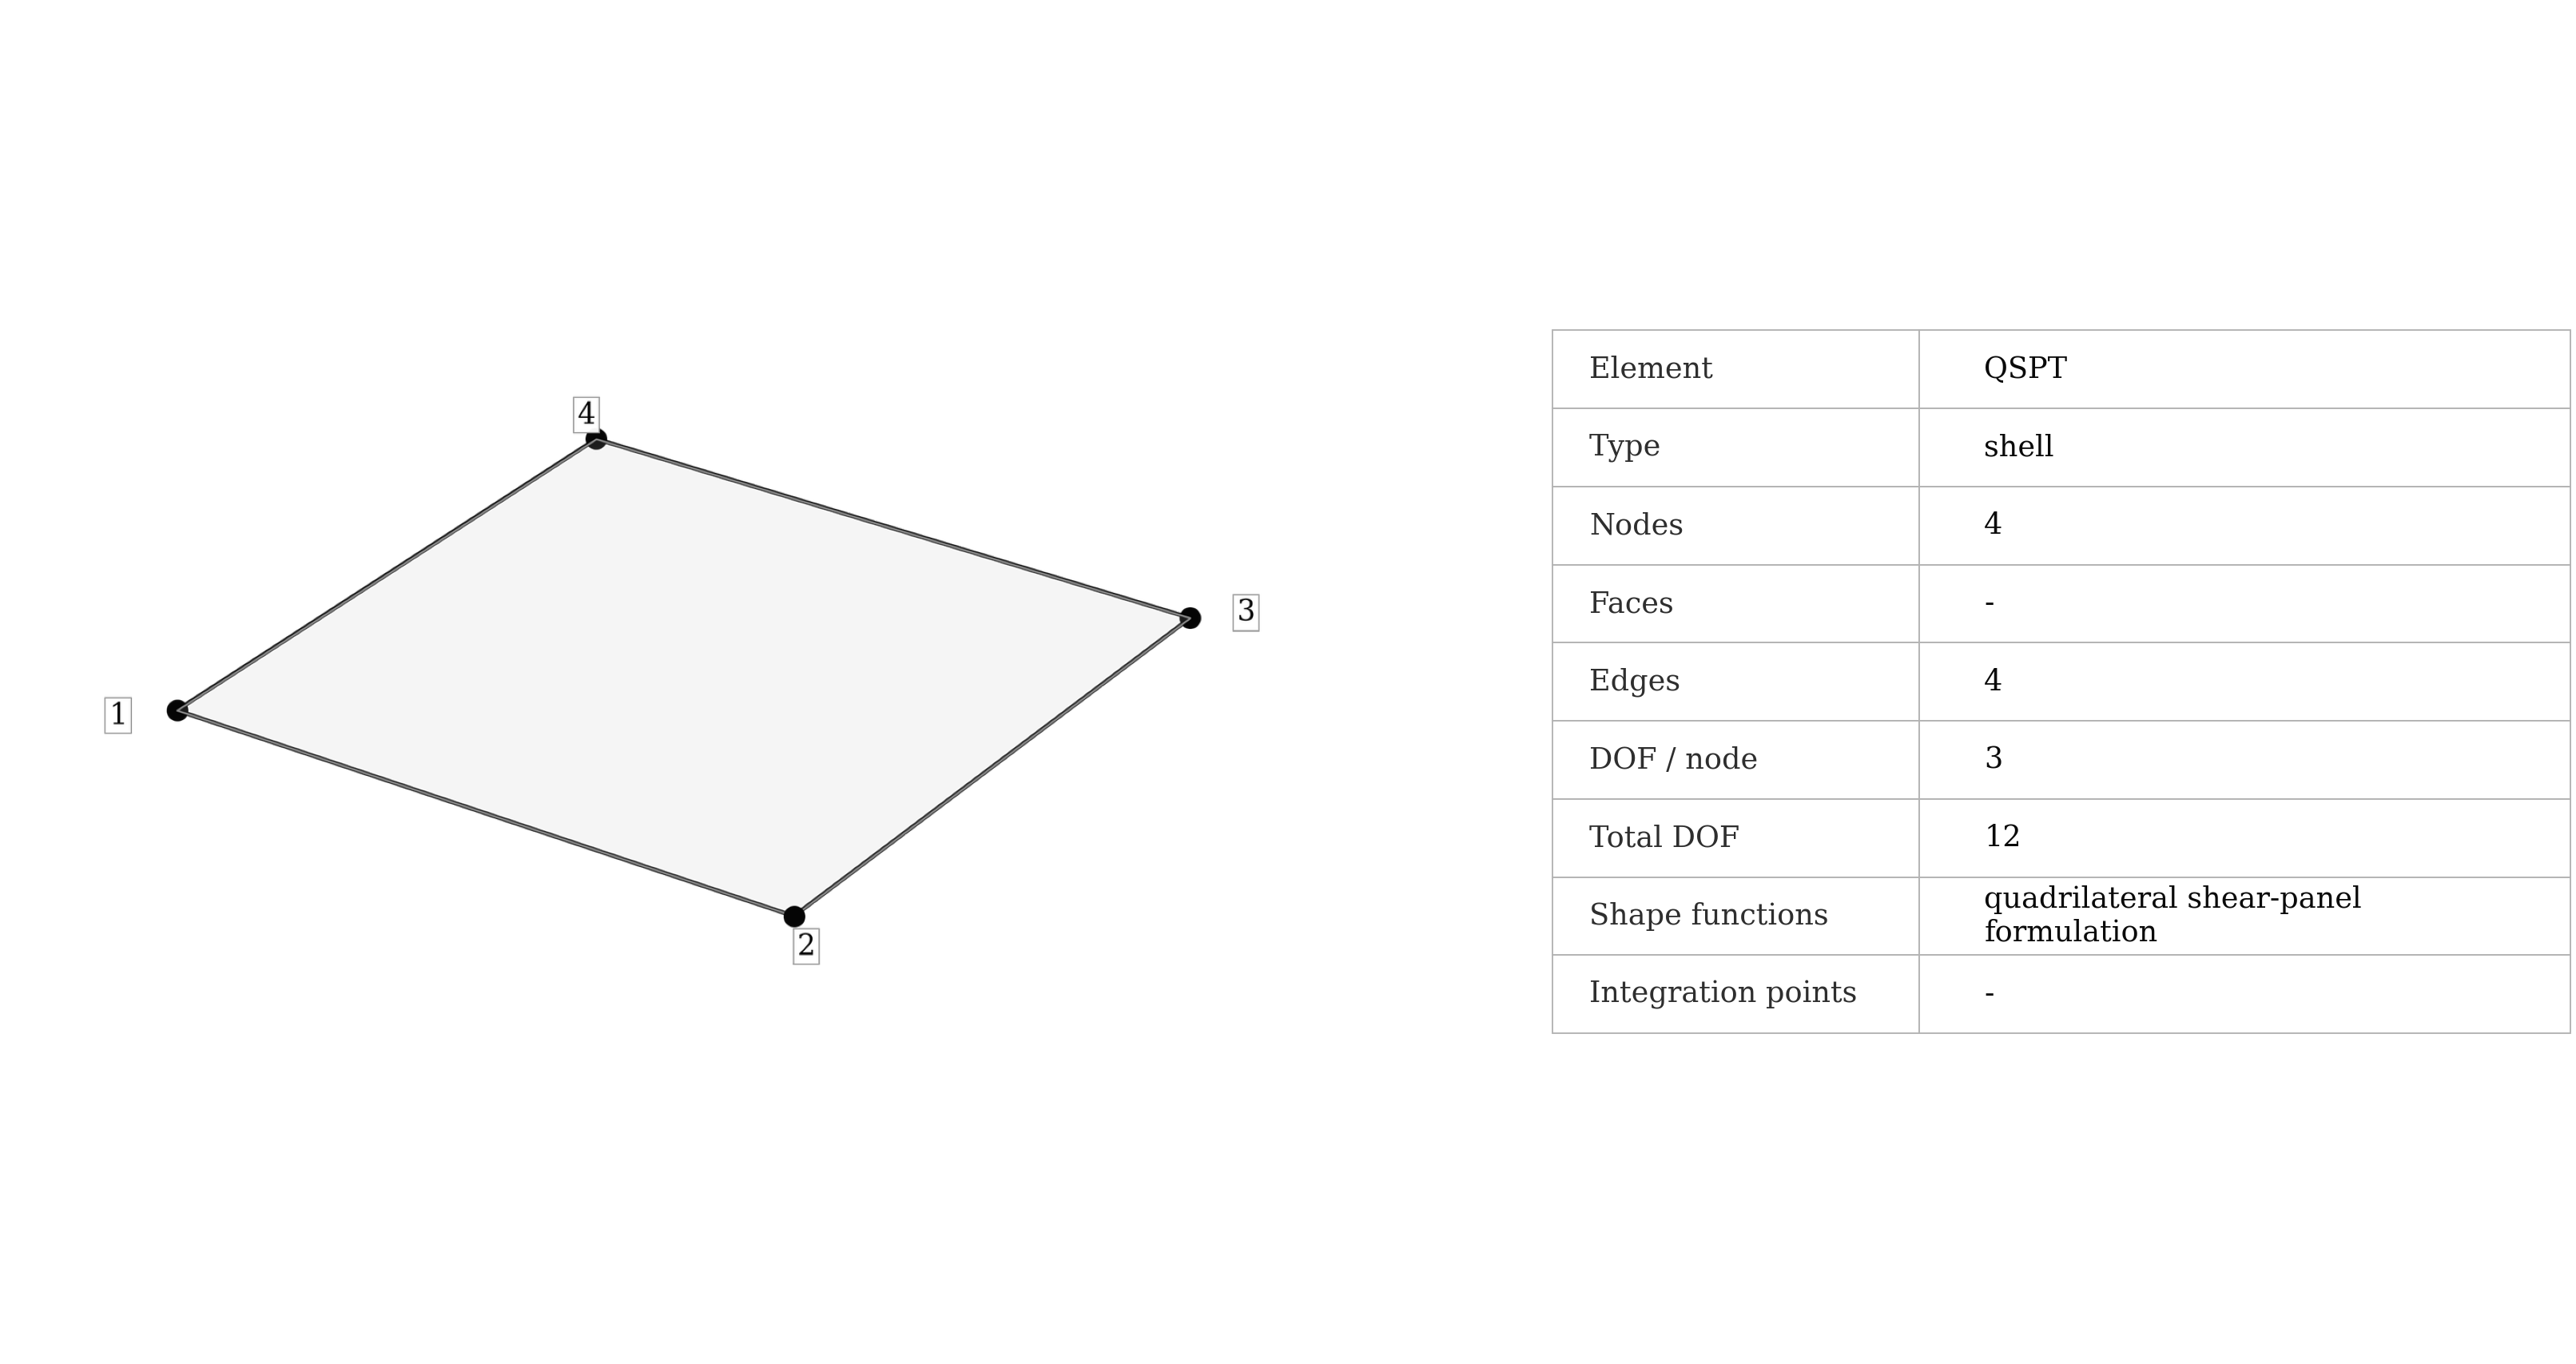
\includegraphics[width=0.78\linewidth]{pages/figures/element_schematics/qspt_schematic.png}
    \caption{\val{QSPT} shear-panel element.}
\end{figure}

\begin{syntax}
*ELEMENT, TYPE=QSPT, ELSET=<set>
<id>, <n1>, <n2>, <n3>, <n4>
\end{syntax}

\val{QSPT} is a specialized four-node quadrilateral panel element developed for shear-flow-oriented structural idealizations. It is intended for simplified panel models where the principal purpose of the element is to transfer in-plane shear rather than reproduce the complete behaviour of a general shell.

Typical applications are preliminary thin-walled structures, webs, aircraft-style shear panels, and reduced-order structural models in which panel shear flow is the primary quantity of interest. In such models \val{QSPT} can provide a compact load-path representation without introducing a complete shell formulation for every panel.

\val{QSPT} is not a general replacement for \val{MITC4FRT} despite sharing a four-node quadrilateral topology. It does not provide the bending stiffness, local shell curvature, full shell resultants, or detailed top/bottom stresses of a shell formulation.

\clearpage
\subsubsection{Beam and truss elements}

Line elements idealize slender three-dimensional members by describing the cross-section through section properties instead of meshing it explicitly. This can reduce the number of degrees of freedom by orders of magnitude compared with shell or solid modelling. The trade-off is that local three-dimensional connection behaviour, detailed cross-section distortion, holes, welds, and local stress concentrations are not resolved.

\clearpage
\paragraph{\val{B31}: 2-node geometrically exact 3D beam}

\begin{syntax}
*ELEMENT, TYPE=B31, ELSET=<set>
<id>, <n1>, <n2>
\end{syntax}

\val{B31} is a two-node shear-flexible spatial beam with three translational and three rotational degrees of freedom per node. The rotational degrees of freedom use FEMaster's total global axis--angle convention. The element evaluates finite rotations on \(SO(3)\), interpolates the relative nodal rotation objectively along the shortest rotation path, and carries the six generalized section strains
\[
[\varepsilon_x,\gamma_y,\gamma_z,\kappa_x,\kappa_y,\kappa_z]^T .
\]

The formulation uses the two end points as order-one Gauss--Lobatto integration points. Axial, transverse-shear, torsional and bending stiffnesses are obtained from the assigned isotropic material and \cmd{PROFILE}. The profile values \(A_{sy}\) and \(A_{sz}\) define the effective shear areas; if they are omitted, both default to \(5A/6\).

Finite section offsets are part of the beam kinematics. With \(SP\) the shear point, \(SMP\) the section material/centroid point and \(REF\) the nodal reference line, the stored profile data define
\[
SP-SMP=(0,e_y,e_z),\qquad
REF-SMP=(0,\mathrm{ref}_y,\mathrm{ref}_z).
\]
The vector from the nodal reference line to the shear point is therefore rotated with the current section orientation. The \(SP-SMP\) eccentricity also enters the sectional constitutive matrix so axial/bending coupling is represented without applying a small-rotation offset matrix after assembly.

For nonlinear static analysis the internal force and the complete tangent are evaluated at the supplied base state. A superposed finite rigid-body translation and rotation therefore produces zero generalized strain. Linear static, eigenfrequency, harmonic and buckling operators use the same B31 reference tangent and mass/geometric operators. The current mass operator is the order-one collocated sectional mass matrix including reference-line eccentricity.

The relative rotation between the two B31 nodes must remain below 180 degrees so the shortest \(SO(3)\) interpolation branch is unique. Large overall rigid-body rotations are not restricted by this condition; it applies only to the relative nodal rotation within one element.

\clearpage
\paragraph{\val{B33}: 3D beam element}

\begin{figure}[H]
    \centering
    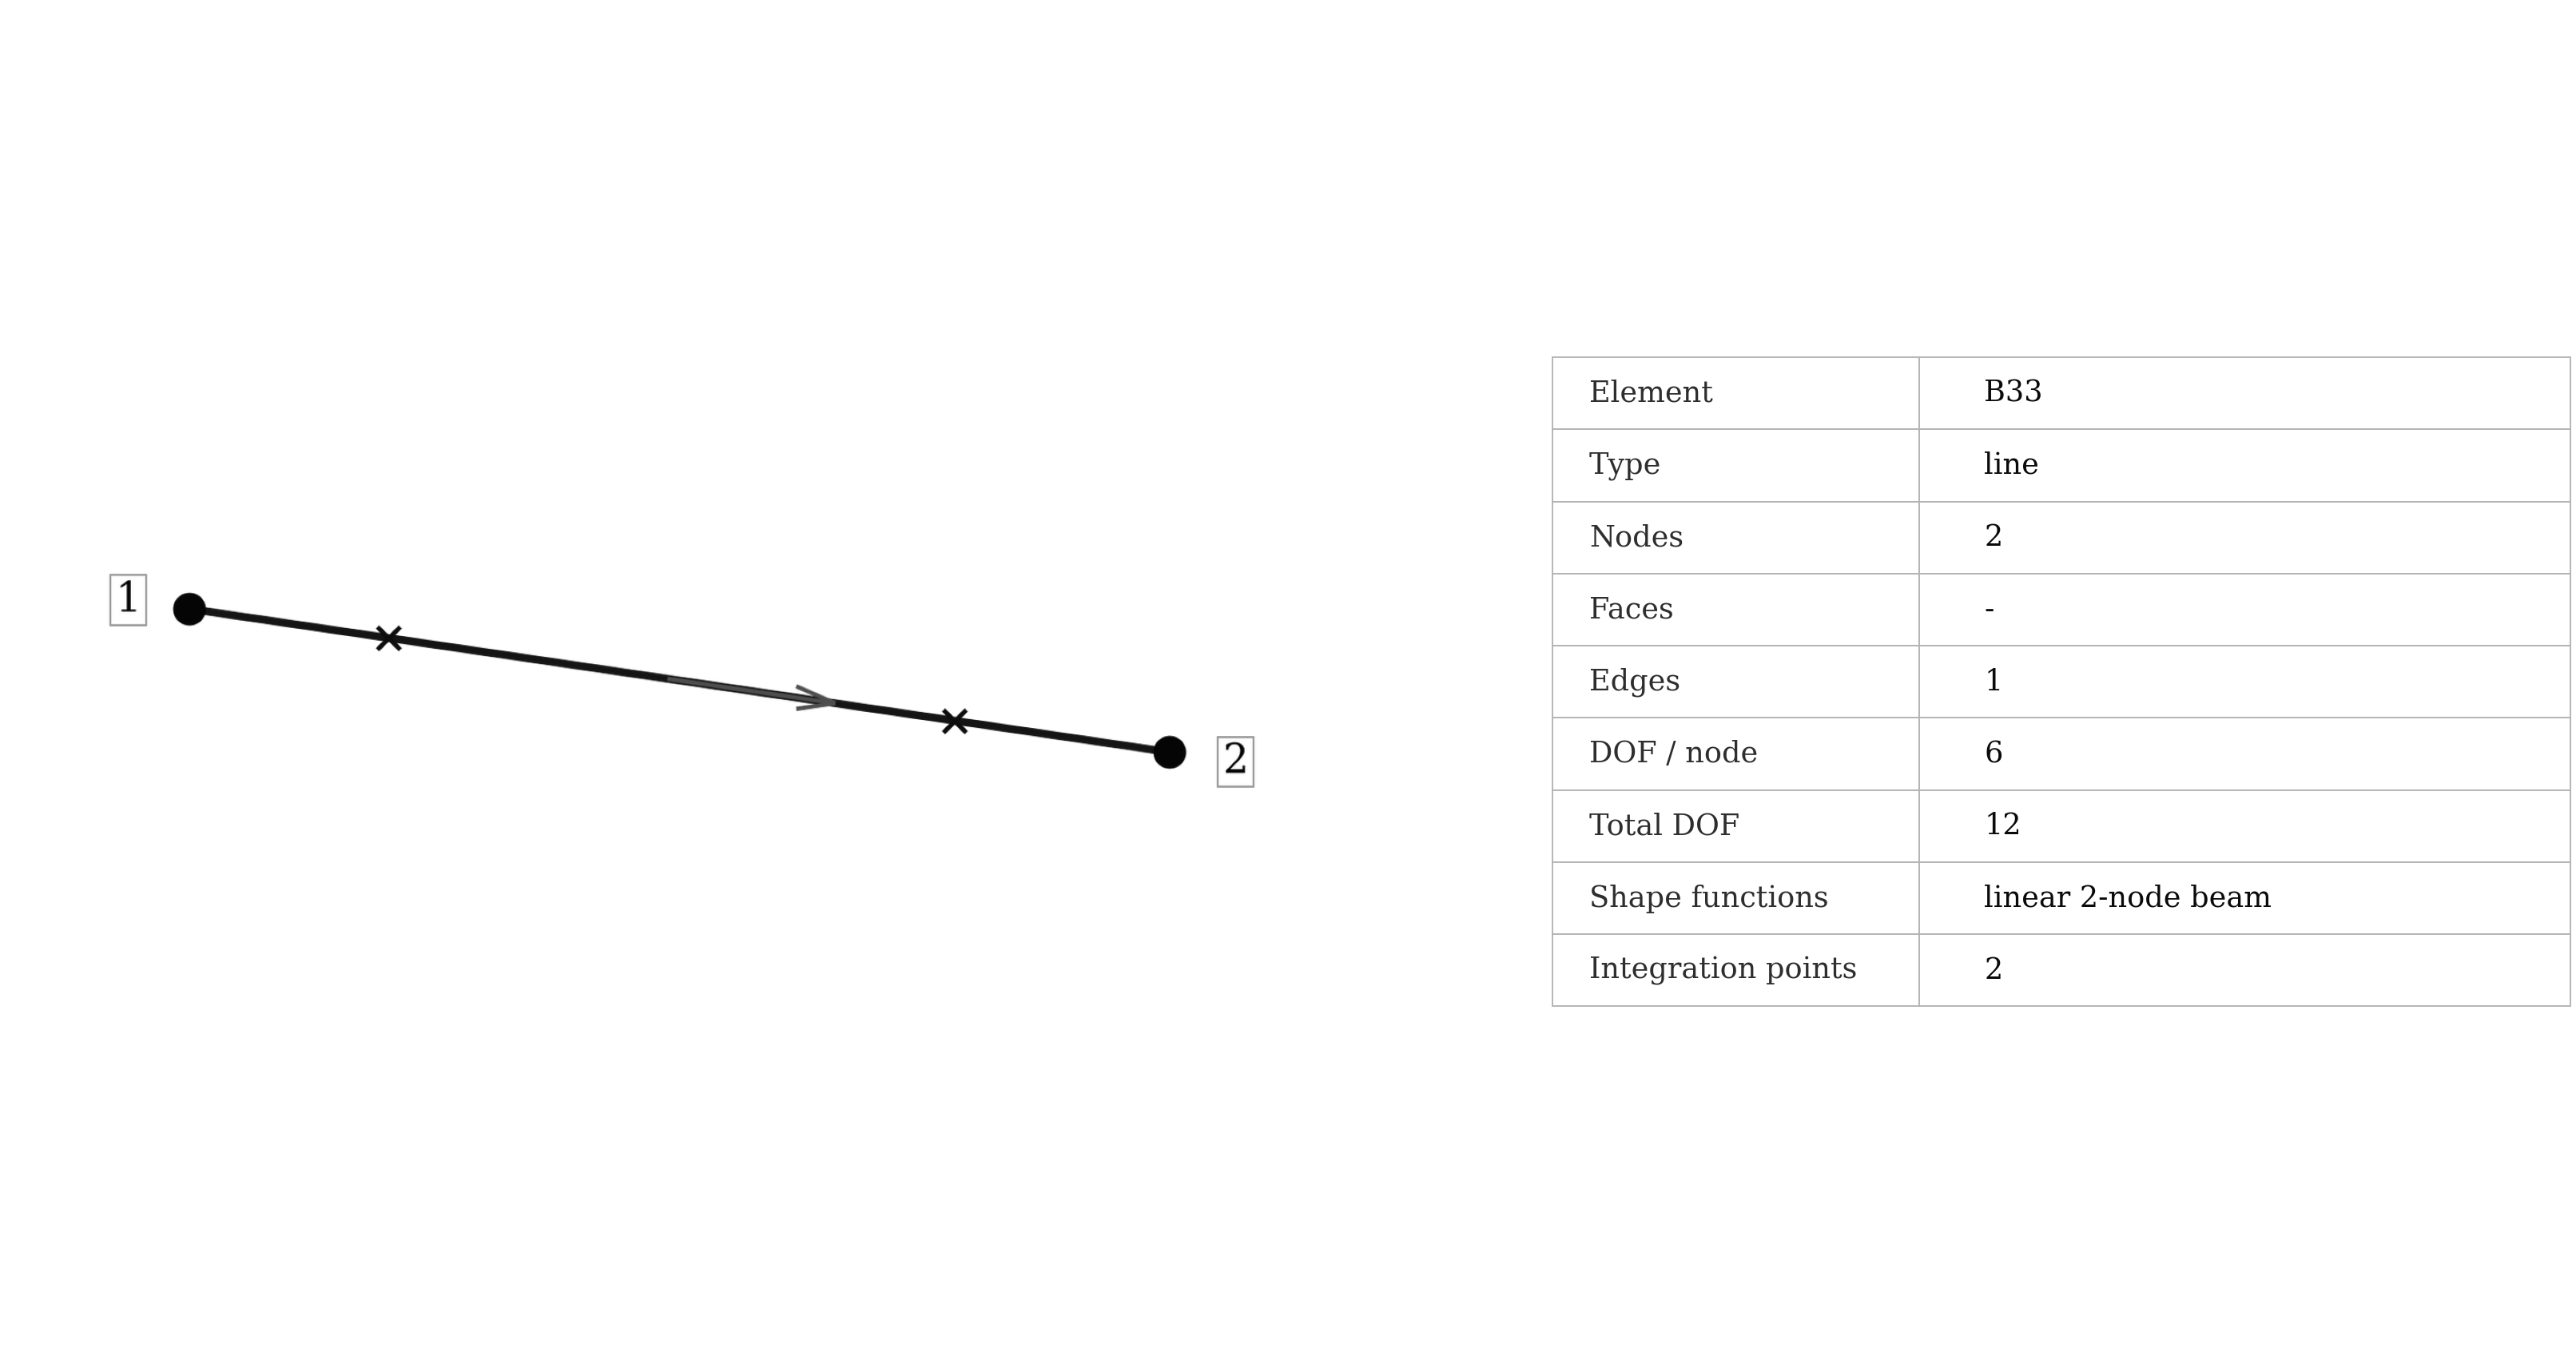
\includegraphics[width=0.70\linewidth]{pages/figures/element_schematics/b33_schematic.png}
    \caption{\val{B33} beam element.}
\end{figure}

\begin{syntax}
*ELEMENT, TYPE=B33, ELSET=<set>
<id>, <n1>, <n2>
\end{syntax}

\val{B33} is a two-node three-dimensional beam element with translational and rotational nodal degrees of freedom. It represents axial deformation, bending, torsion, and the section response defined by \cmd{BEAM SECTION} and the referenced \cmd{PROFILE}.

The current \cmd{ELEMENT} syntax uses exactly two connectivity nodes for \val{B33}. Beam cross-section orientation is supplied by the orientation vector in \cmd{BEAM SECTION}; an additional orientation node is not part of the current connectivity grammar.

Beam elements represent slender frames, stiffeners, spars, ribs, idealized support members, and other structures through Section forces and global deformation. They include axial area, bending inertias, torsional stiffness, product of inertia, Section offsets, and reference-line offsets without meshing the full cross-section.

The beam idealization does not resolve local connection stresses, bolt or weld geometry, detailed cross-section deformation, or three-dimensional load introduction. Those effects require a corresponding shell or solid representation. The beam local axes determine the interpretation of bending moments, section forces, and profile properties.

The Abaqus-compatible \val{B33} name uses the same two-node connectivity.

\clearpage
\paragraph{\val{T3}: 2-node truss element}

\begin{figure}[H]
    \centering
    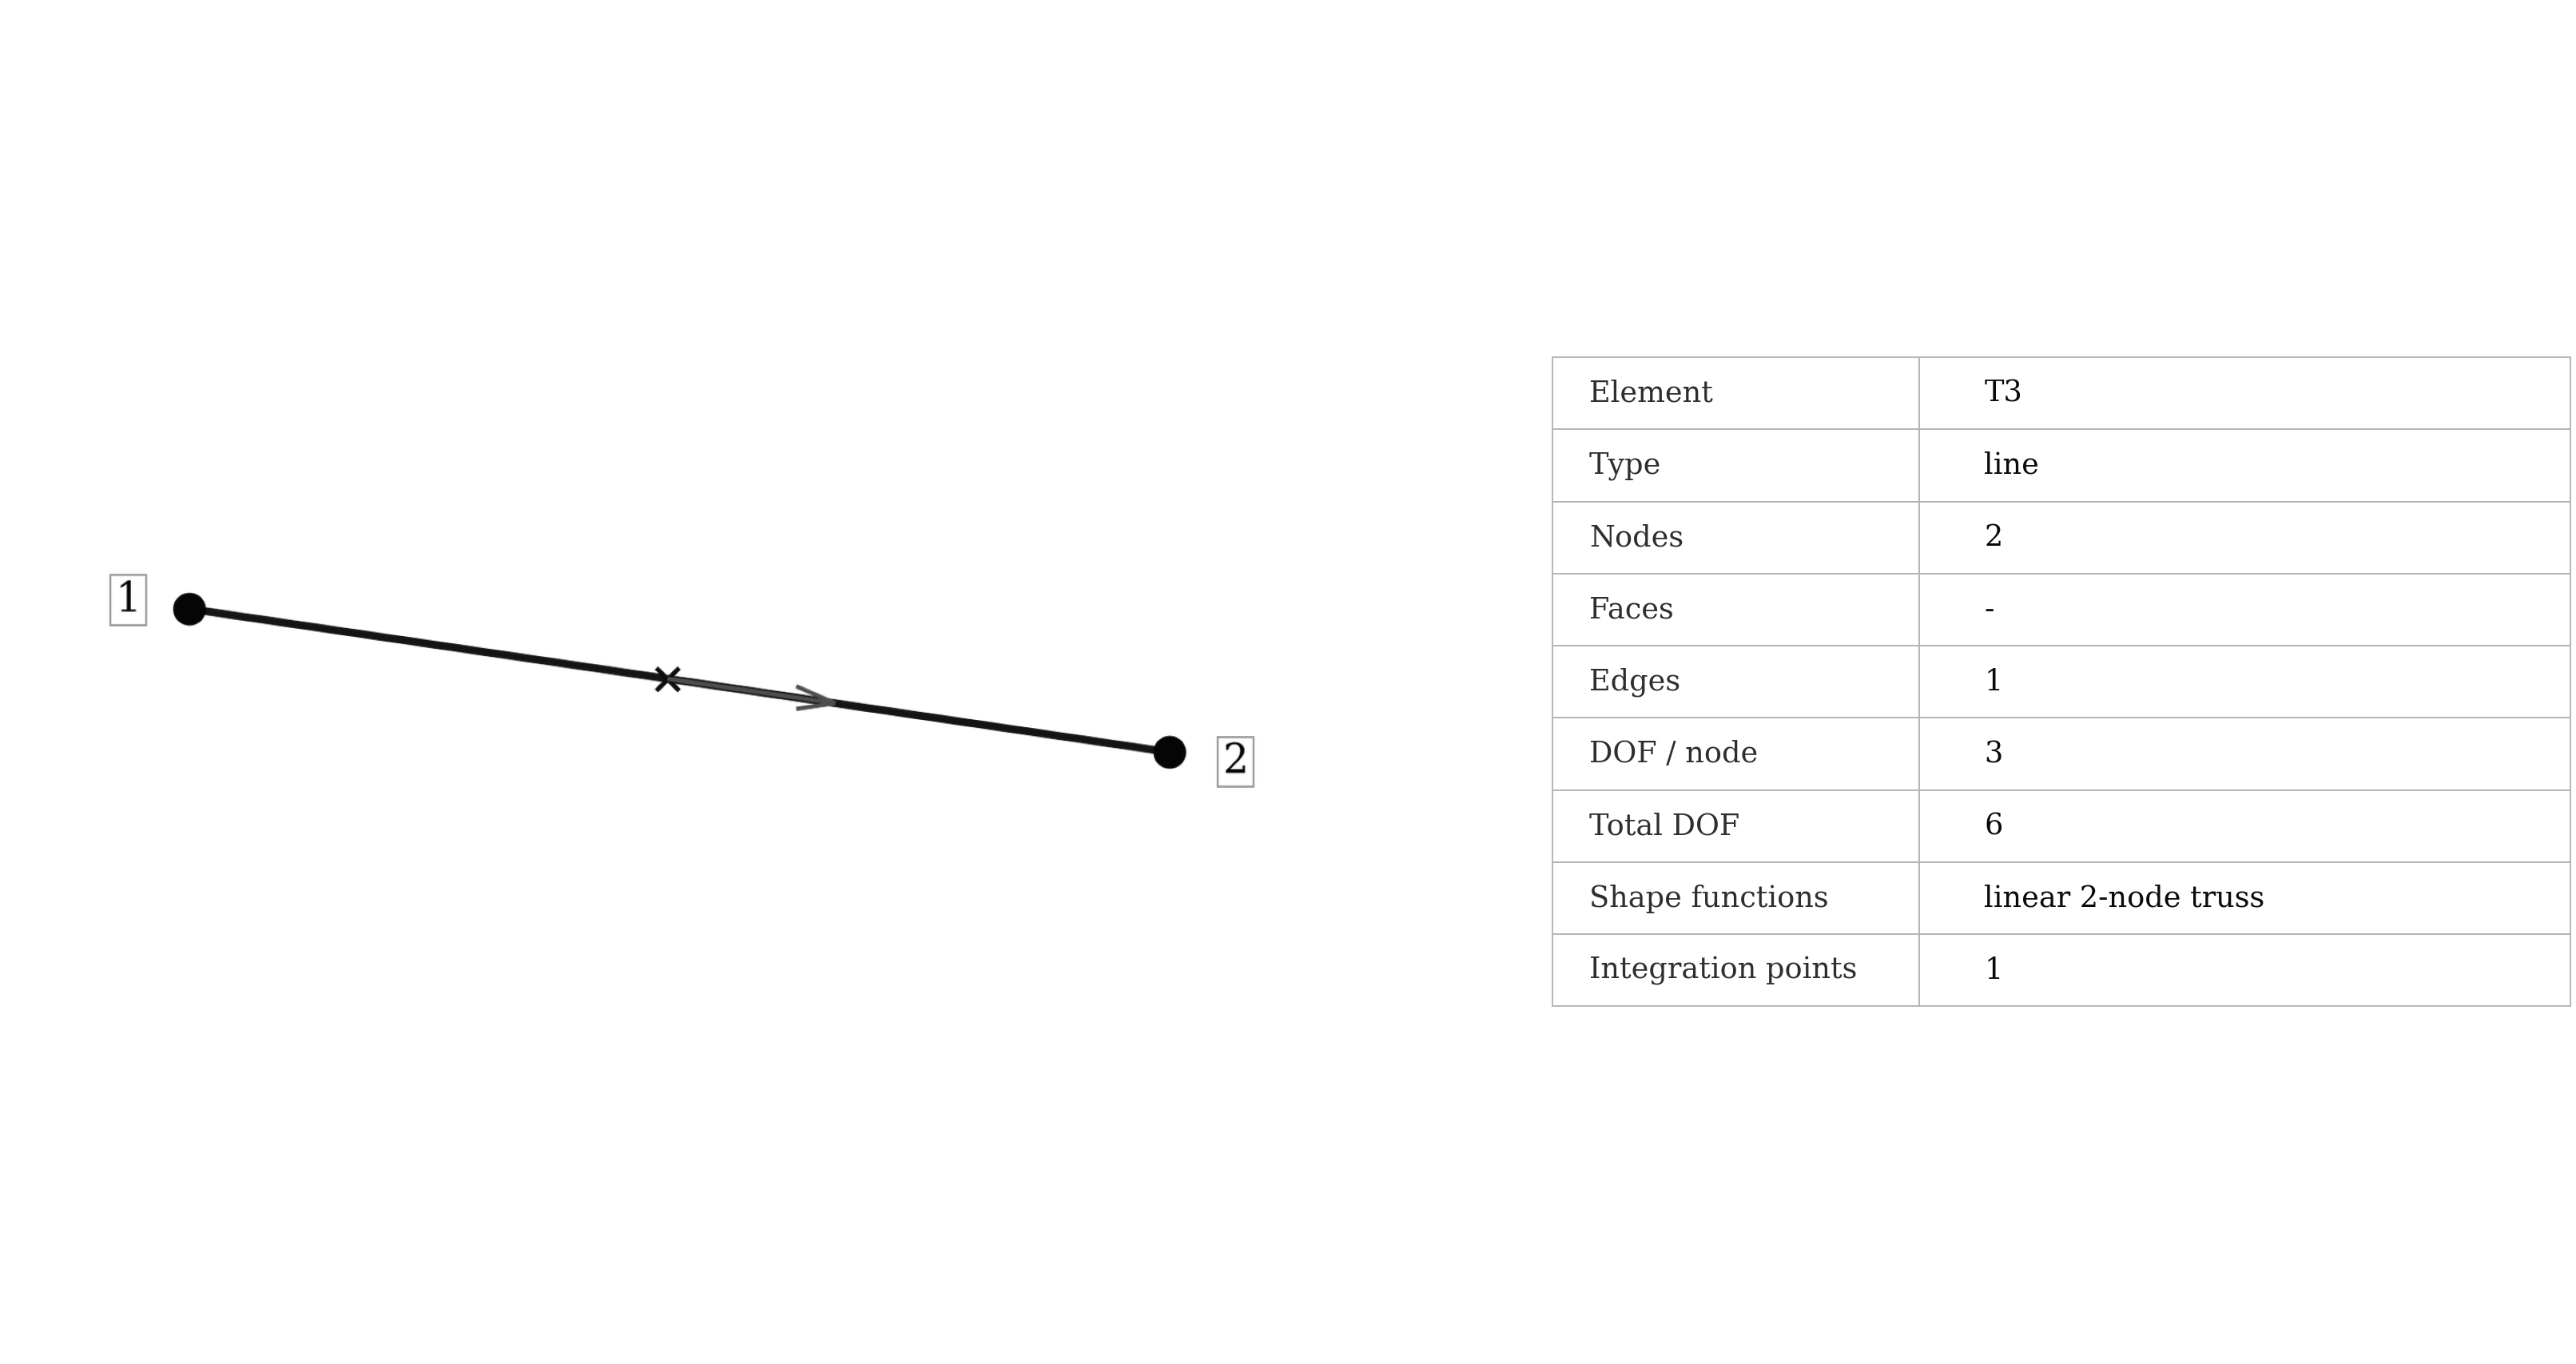
\includegraphics[width=0.68\linewidth]{pages/figures/element_schematics/t3_schematic.png}
    \caption{\val{T3} truss element.}
\end{figure}

\begin{syntax}
*ELEMENT, TYPE=T3, ELSET=<set>
<id>, <n1>, <n2>
\end{syntax}

\val{T3} is a two-node truss element. It carries axial force along its current line direction and uses translational nodal degrees of freedom. The material and cross-sectional area are assigned by \cmd{TRUSS SECTION}.

The element represents pin-jointed members, rods, braces, links, and other components whose structural action is axial tension or compression. Its mechanical quantities are axial force, axial strain, and axial stress.

The limitations are deliberate. \val{T3} has no bending stiffness, no torsional stiffness, and no rotational continuity. It cannot model fixed-end moments, eccentric frame action, or transverse stiffness of a physical beam; those behaviours require \val{B33} or a shell/solid representation.

The Abaqus-compatible name \val{T3D2} selects the same FEMaster truss formulation as \val{T3}.

\begin{inputdeck}[Abaqus-compatible alternative]
*ELEMENT, TYPE=T3D2, ELSET=BARS
10, 1, 2
\end{inputdeck}

\clearpage
\subsubsection{Point elements}

Point elements are zero-dimensional structural elements attached to a single node. They preserve element identity and ELSET membership while their physical contribution is supplied by an assigned point-mass section rather than by continuum geometry or a material law. The unified input language accepts three regular one-node types: \val{MASS}, \val{ROTARYI}, and \val{SPRING1}. Internally all three use the same \texttt{PointElement}; the corresponding property keyword determines which generalized diagonal coefficient is populated.

A point element without an assigned point property is intentionally inert. It has zero stiffness, zero mass, no stress or strain state, and activates no degrees of freedom. Property definitions are documented in Section~\ref{sec:sections}; this section focuses on the element topology and kinematic role.

\clearpage
\paragraph{\val{MASS}: 1-node concentrated-mass element}

\begin{syntax}
*ELEMENT, TYPE=MASS, ELSET=<set>
<id>, <node>
*MASS, ELSET=<set>
<mass>
\end{syntax}

\val{MASS} is an Abaqus-compatible one-node point element. The \cmd{ELEMENT} record creates only topology: an element ID, one connected node, and normal ELSET membership. The scalar physical mass is assigned separately by \cmd{MASS, ELSET=...}.

For the supported isotropic property, the element mass matrix is
\[
M_e=\operatorname{diag}(m,m,m,0,0,0),
\]
so a positive mass activates the three translational components at the connected node. Several \val{MASS} elements may reference the same node; each represents an independent concentrated contribution and the assembled mass is additive.

The point element has zero geometric volume, but its density-scaled field integration interprets \(m\) as the complete concentrated mass measure. Consequently, a regular \val{MASS} element contributes to the global mass matrix, eigenfrequency and transient analyses, inertia relief, and element-targeted mass-proportional body or inertial loads. The Abaqus-compatible \cmd{DLOAD} with \val{GRAV} produces the concentrated force \(m\boldsymbol a\) when the selected element region contains the point element. FEMaster-specific \cmd{VLOAD} instead denotes force density and does not load this zero-volume point element.

Part-local \val{MASS} elements and their \cmd{MASS} property assignments are copied to every Instance during model compilation. An assembly-level \cmd{MASS} assignment instead targets compiled point elements through an assembly ELSET.

\textbf{Alternative:} For concentrated mass that does not require
an explicit element ID or ELSET membership, the FEMaster-specific
\cmd{POINTMASS} keyword assigns a mass directly to an NSET:

\begin{inputdeck}[FEMaster-specific alternative]
*POINTMASS, NSET=PAYLOAD_NODES
0.025
\end{inputdeck}

This creates auxiliary point elements during model compilation.
The specified value is applied independently to each node in the
set; load selection and element-set behavior differ from a regular
\val{MASS} element. See Section~\ref{sec:sections}.

\clearpage
\paragraph{\val{ROTARYI}: 1-node rotary-inertia element}

\begin{syntax}
*ELEMENT, TYPE=ROTARYI, ELSET=<set>
<id>, <node>
*ROTARY INERTIA, ELSET=<set>
<I11>, <I22>, <I33>, <I12>, <I13>, <I23>
\end{syntax}

\val{ROTARYI} is the rotational-inertia counterpart of \val{MASS}. Its one-node topology is identical, but the property acts on the rotational degrees of freedom. FEMaster's supported diagonal mapping produces
\[
M_e=\operatorname{diag}(0,0,0,I_{11},I_{22},I_{33}).
\]
Each nonzero diagonal inertia activates its corresponding nodal rotation.

Abaqus permits the full symmetric rotary-inertia tensor. The current FEMaster point section stores only the diagonal moments, so the data positions \(I_{12}\), \(I_{13}\), and \(I_{23}\) are accepted only when zero. Orientation-dependent rotary inertia is likewise outside the current mapping.

A \val{ROTARYI} element can share its connected node with a \val{MASS} element. This is the regular element-based way to represent translational mass and rotary inertia at the same physical point while preserving the Abaqus separation between the two element families.

\clearpage
\paragraph{\val{SPRING1}: 1-node point-to-ground spring}

\begin{syntax}
*ELEMENT, TYPE=SPRING1, ELSET=<set>
<id>, <node>
*SPRING, ELSET=<set>
<dof>
<stiffness>
\end{syntax}

\val{SPRING1} is a one-node spring between the connected node and ground. The first \cmd{SPRING} data line selects the generalized nodal direction; the second gives the constant linear stiffness. Degrees of freedom 1--3 act on translations and degrees of freedom 4--6 act on rotations.

For one selected direction the point-element stiffness matrix contains exactly one nonzero diagonal entry. Translational DOFs therefore represent ordinary point-to-ground springs, whereas rotational DOFs represent torsional point-to-ground springs. Multiple independent directions are represented by multiple \val{SPRING1} elements, which may all reference the same node.

The current mapping is deliberately narrower than the complete Abaqus spring family. It supports only real, constant, linear \val{SPRING1} behavior in the global nodal system. \val{SPRING2}, \val{SPRINGA}, local orientations, nonlinear force--displacement curves, frequency or field dependence, and complex stiffness are not mapped.

The FEMaster-specific \cmd{POINTMASS} keyword provides an alternative NSET-based convenience syntax when mass, rotary inertia, and several diagonal translational or rotational springs should be combined directly on the same target nodes. It creates auxiliary post-compile point elements rather than regular ELSET members.

\addtocontents{toc}{\protect\setcounter{tocdepth}{3}}


\keywordpage{NSET}

\cmd{NSET} creates or extends a named node set. The same basic syntax is accepted by native FEMaster and by the supported Abaqus input format. \key{NSET} gives the set name; \key{NAME} is accepted as an alternative spelling. Data may contain explicit node references or generated arithmetic ranges.

Inside a Part, numerical entries refer to that Part's local node IDs. Separate Parts may therefore contain sets with the same numerical members without referring to the same physical nodes. If a Part is instantiated more than once, its Part-level node sets remain available for every copy.

At Assembly level, \key{INSTANCE=<name>} qualifies local IDs with one particular Instance. This is the most direct way to create a support or load region on one placed copy of a reusable Part. Assembly-level sets may also combine selections from different Instances by using the supported qualified references or by building larger sets from previously named regions.

With \key{GENERATE}, every data row contains
\[
\text{start},\quad \text{end},\quad \text{increment}.
\]
The end value is inclusive. The increment defaults to 1 and must not be zero. Positive and negative increments are supported, so generated sequences can run in either direction as long as the sign agrees with the requested range.

Part-level sets represent regions intrinsic to the component, such as a bolt row, root edge, or material domain, and are available on every Instance. Assembly-level sets represent placement-dependent selections, such as one support on a particular Instance or a region combining nodes from several components.

\begin{keywordparameters}
\key{NSET} / \key{NAME} & required & Name of the node set to create or extend. \\
\key{INSTANCE} & optional & Assembly-level qualifier for local node references. \\
\key{GENERATE} & optional flag & Interpret each data row as start, end, increment. \\
\end{keywordparameters}

\begin{keyworddata}
Explicit form & One or more node IDs or supported named/qualified node references. \\
Generated form & \val{start, end, increment}; the increment defaults to \val{1} and must be nonzero. \\
\end{keyworddata}

\exampleheading

\begin{dialectexamples}
\begin{femasterdeck}
*PART, NAME=BEAM
*NODE
0, 0., 0., 0.
1, 1., 0., 0.
2, 2., 0., 0.
3, 3., 0., 0.
*NSET, NSET=ENDS
0, 3
*NSET, NSET=ALLN, GENERATE
0, 3, 1
*END PART
\end{femasterdeck}
\begin{abaqusdeck}
*PART, NAME=BEAM
*NODE
0, 0., 0., 0.
1, 1., 0., 0.
2, 2., 0., 0.
3, 3., 0., 0.
*NSET, NSET=ENDS
0, 3
*NSET, NSET=ALLN, GENERATE
0, 3, 1
*END PART
\end{abaqusdeck}
\end{dialectexamples}

\clearpage
\paragraph*{Assembly-level Instance selection}

A typical Assembly selection looks like
\begin{syntax}
*ASSEMBLY
*INSTANCE, NAME=BEAM_A, PART=BEAM
0., 0., 0.
*END INSTANCE
*INSTANCE, NAME=BEAM_B, PART=BEAM
100., 0., 0.
*END INSTANCE

*NSET, NSET=SUPPORT_A, INSTANCE=BEAM_A
0
*NSET, NSET=SUPPORT_B, INSTANCE=BEAM_B
0
*END ASSEMBLY
\end{syntax}
Both sets contain a local node with ID \val{0}, but they refer to different placed Instances.

\keywordpage{ELSET}

\cmd{ELSET} is the element-domain counterpart of \cmd{NSET}. It creates or extends a named element set from explicit element references or generated ranges. \key{ELSET} supplies the name and \key{NAME} is accepted as an alternative.

Element sets are central to property assignment. Solid, shell, beam, and truss Sections normally target an \cmd{ELSET}, so the element-set structure can mirror the physical construction of the model through separate names for different materials, thicknesses, beam profiles, or design domains.

Inside a Part, entries refer to that Part's local element IDs. At Assembly level, \key{INSTANCE} qualifies local IDs with one placed Instance. This allows two Instances of the same Part to be selected independently even though they use identical local element numbering.

\key{GENERATE} follows the same inclusive start/end/increment rule as \cmd{NSET}. ID \val{0} is valid, so for example \val{0, 99, 1} generates one hundred element IDs if they exist in the intended topology.

A Section assigned to a Part-level element set belongs to the component and follows every Instance of the Part. Assembly-level element sets instead identify loads, diagnostics, or other selections whose meaning depends on the particular placed copy.

\begin{keywordparameters}
\key{ELSET} / \key{NAME} & required & Name of the element set to create or extend. \\
\key{INSTANCE} & optional & Assembly-level qualifier for local element references. \\
\key{GENERATE} & optional flag & Generate an arithmetic sequence of element IDs. \\
\end{keywordparameters}

\begin{keyworddata}
Explicit form & One or more element IDs or supported named/qualified element references. \\
Generated form & \val{start, end, increment}; inclusive end, nonzero increment. \\
\end{keyworddata}

\exampleheading

\begin{dialectexamples}
\begin{femasterdeck}
*ELSET, ELSET=DESIGN_DOMAIN, GENERATE
0, 99, 1

*ELSET, ELSET=EVEN_ELEMENTS, GENERATE
0, 98, 2
\end{femasterdeck}
\begin{abaqusdeck}
*ELSET, ELSET=DESIGN_DOMAIN, GENERATE
0, 99, 1

*ELSET, ELSET=EVEN_ELEMENTS, GENERATE
0, 98, 2
\end{abaqusdeck}
\end{dialectexamples}

\keywordpage{SURFACE}

\cmd{SURFACE} defines a geometric boundary from element sides. A surface is more than a node set: it retains which element face is selected and therefore has a well-defined interpolation, area or line measure, and orientation. Surface information is required for pressure loads, distributed tractions, surface couplings, ties, and contact.

A side is selected by an element or element-set target together with a side label such as \val{S1}, \val{S2}, and so on. The actual face represented by a side label depends on the element type and its connectivity. Reversing or changing the element node order can therefore change the physical direction of a surface normal.

For shell elements the two sides of the midsurface can also be described by \val{SPOS} and \val{SNEG}. These represent the positive and negative shell sides that determine pressure direction and top/bottom interpretation.

Native FEMaster additionally supports an explicit surface-ID form in which a user surface ID is supplied together with the parent element and side. Explicit surface IDs are non-negative and may start at \val{0}. A surface named directly from an element or element set avoids the separate numerical surface-ID space of the explicit form.

At Assembly level, \key{INSTANCE} can qualify the target element or element set. This allows a face of one particular Instance to be selected even when several copies use the same local element IDs and set names.

The Abaqus example uses the supported element-based \cmd{SURFACE, TYPE=ELEMENT} syntax. Only the specialized surface features documented here are included in the supported Abaqus subset.

An unordered node set contains no element-side information and therefore cannot define a pressure or contact normal. The selected element side determines the surface orientation. For shell models, normal consistency additionally controls the positive and negative shell faces and the sign convention of bending-related quantities.

\begin{keywordparameters}
\key{SFSET} / \key{NAME} & optional & Name of the destination surface region; native default \val{SFALL}. \\
\key{INSTANCE} & optional & Assembly-level Instance qualifier. \\
\end{keywordparameters}

\begin{keyworddata}
Target form & \val{element-or-elset, side}. \\
Explicit native form & \val{surface_id, element_id, side}. \\
\end{keyworddata}

\exampleheading

\begin{dialectexamples}
\begin{femasterdeck}
*SURFACE, NAME=TOP
SOLIDS, S2

*SURFACE, NAME=ONE_FACE
0, 42, S1
\end{femasterdeck}
\begin{abaqusdeck}
*SURFACE, NAME=TOP, TYPE=ELEMENT
SOLIDS, S2
\end{abaqusdeck}
\end{dialectexamples}

\keywordpage{SFSET}

\cmd{SFSET} groups existing native FEMaster surface entities into a named surface region. It combines surfaces created with explicit user surface IDs or several previously defined surface groups into one target.

\cmd{SURFACE} and \cmd{SFSET} therefore serve different purposes: \cmd{SURFACE} creates geometric boundary entities from elements, while \cmd{SFSET} collects already existing surface entities. A direct named \cmd{SURFACE} does not require the separate numerical surface-ID space used by \cmd{SFSET}.

The destination name is supplied by \key{SFSET} or \key{NAME}; the native default is \val{SFALL}. Explicit surface references can be listed directly. With \key{GENERATE}, arithmetic ranges of surface IDs can be produced using the same inclusive start/end/increment convention as node and element sets. \key{INSTANCE} can be used for Assembly-level selection where applicable.

The supported Abaqus input format does not have a separate \cmd{SFSET} keyword. A named Abaqus \cmd{SURFACE} already serves as the reusable surface region, so the right-hand example expresses the same modelling intent directly through one combined surface definition.

\begin{keywordparameters}
\key{SFSET} / \key{NAME} & optional & Destination surface-region name; native default \val{SFALL}. \\
\key{INSTANCE} & optional & Assembly-level Instance qualifier. \\
\key{GENERATE} & optional flag & Generate an arithmetic sequence of surface IDs. \\
\end{keywordparameters}

\begin{keyworddata}
Explicit form & Existing surface IDs or supported named surface references. \\
Generated form & \val{start, end, increment}; inclusive end, nonzero increment. \\
\end{keyworddata}

\exampleheading

\begin{dialectexamples}
\begin{femasterdeck}
*SURFACE, NAME=PATCH_A
0, 20, S1
1, 21, S1
*SURFACE, NAME=PATCH_B
2, 22, S1

*SFSET, NAME=CONTACT_FACE
0, 1, 2
\end{femasterdeck}
\begin{abaqusdeck}
*SURFACE, NAME=CONTACT_FACE, TYPE=ELEMENT
20, S1
21, S1
22, S1
\end{abaqusdeck}
\end{dialectexamples}


\section{Model Properties}
\label{sec:model-properties}
\subsection{Materials}
\label{sec:materials}

Materials define constitutive and inertial properties independently of the mesh. A material is created once, given a name, and referenced by one or more Sections. The same material may therefore be used by several element regions, Parts, or Instances without duplicating its constants.

\cmd{MATERIAL} begins a material definition. The material-property keywords that follow---for example \cmd{ELASTIC}, \cmd{PLASTIC}, \cmd{HYPERELASTIC}, \cmd{DENSITY}, and thermal expansion---belong to that material until the material definition ends with the next appropriate root-level model definition. A material may contain only the properties required by the intended analyses; for example, density is unnecessary for a purely elastic static stiffness calculation but is required when mass participates in the mechanics.

\keywordnestedpage{MATERIAL}

\cmd{MATERIAL} creates a named material and makes it the current target for subsequent material-property keywords. Native FEMaster accepts the identifier through \key{MATERIAL} or \key{NAME}; Abaqus input uses \key{NAME}.

The command itself does not define a constitutive law. Elasticity, plasticity, hyperelasticity, density, and thermal expansion are added with separate keywords. This makes the material definition modular and keeps the physical meaning of each property explicit.

Material names must be unique. Sections reference the material by name, so one definition can be reused throughout the model.

Materials are independent of Parts. The corresponding Section assignment connects a material to a particular mesh region.

\begin{keywordparameters}
\key{MATERIAL} / \key{NAME} & required & Unique material identifier. \\
\end{keywordparameters}

The material definition becomes the active target for ELASTIC and DENSITY. The assigned unit system must be consistent with all geometry, loads, and mass data.

\exampleheading

\begin{inputdeck}
*MATERIAL, NAME=STEEL
*ELASTIC
210000., 0.3
*DENSITY
7.85e-9
\end{inputdeck}


\keywordnestedpage{ELASTIC}

\cmd{ELASTIC} defines a linear-elastic constitutive law. Native FEMaster supports isotropic elasticity, generalized isotropic elasticity with an independent shear modulus, orthotropic engineering constants, and an orthotropic stiffness-coefficient form. The supported Abaqus input covers the corresponding documented Abaqus forms.

\paragraph*{Isotropic elasticity}

For \key{TYPE=ISOTROPIC} or \val{ISO}, the data are Young's modulus \(E\) and Poisson's ratio \(\nu\). This is the default form. The shear modulus is
\[
G=\frac{E}{2(1+\nu)},
\]
and the three-dimensional isotropic constitutive law follows from \(E\) and \(\nu\) in the usual way.

For ordinary stable isotropic elasticity, \(E>0\) and \(-1<\nu<0.5\). Values very close to \(\nu=0.5\) describe nearly incompressible behaviour and may require element formulations and meshes that can represent that regime without excessive volumetric locking.

\paragraph*{Generalized isotropic elasticity}

Native FEMaster also accepts \val{GENERALISEDISOTROPIC}, \val{GENERALISED_ISOTROPIC}, or \val{GENISO}. This form reads \(E\), \(\nu\), and an independent \(G\). It preserves the isotropic-style normal relation while allowing the shear response to differ from the classical identity \(G=E/[2(1+\nu)]\).

This is a FEMaster-specific convenience for constitutive models with a physically independent shear modulus. It does not compensate for an inappropriate element formulation or mesh.

\paragraph*{Orthotropic engineering constants}

\key{TYPE=ENGINEERINGCONSTANTS} defines the nine constants
\[
E_1,E_2,E_3,\nu_{12},\nu_{13},\nu_{23},G_{12},G_{13},G_{23}.
\]
These quantities are expressed in the material coordinate system. A Section orientation therefore determines which physical directions of the model correspond to material axes 1, 2, and 3.

The Poisson ratios are directional. For example, \(\nu_{12}\) describes strain in direction 2 caused by stress in direction 1. The reciprocal values follow from elastic symmetry, e.g.
\[
\frac{\nu_{12}}{E_1}=\frac{\nu_{21}}{E_2}.
\]
Transferred orthotropic data are compatible only when the axis ordering and Poisson-ratio convention agree with this definition.

\paragraph*{Orthotropic stiffness coefficients}

\key{TYPE=ORTHOTROPIC} or \val{ORTHO} accepts the nine coefficients
\[
D_{1111},D_{1122},D_{2222},D_{1133},D_{2233},D_{3333},D_{1212},D_{1313},D_{2323}.
\]
The first six values form the symmetric normal-stiffness block
\[
\begin{bmatrix}
D_{1111} & D_{1122} & D_{1133}\\
D_{1122} & D_{2222} & D_{2233}\\
D_{1133} & D_{2233} & D_{3333}
\end{bmatrix},
\]
while \(D_{1212}\), \(D_{1313}\), and \(D_{2323}\) are the three shear stiffnesses. The normal block must be nonsingular. This form accepts constitutive stiffness coefficients directly rather than through engineering constants.

Elastic constants follow the unit system of the model. If stresses are measured in MPa, the elastic moduli and stiffness coefficients are also entered in MPa. FEMaster does not attach units to numerical values, so dimensional consistency is determined by the complete set of input quantities.

\begin{keywordparameters}
\key{TYPE} & optional & Elasticity form. Native default \val{ISOTROPIC}; supported forms and aliases are described above. \\
\end{keywordparameters}

\begin{keyworddata}
\val{E, nu} & Isotropic Young's modulus and Poisson ratio. \\
\val{E, nu, G} & Native generalized-isotropic form. \\
Engineering constants & \(E_1,E_2,E_3,\nu_{12},\nu_{13},\nu_{23},G_{12},G_{13},G_{23}\). \\
Orthotropic stiffness & \(D_{1111},D_{1122},D_{2222},D_{1133},D_{2233},D_{3333},D_{1212},D_{1313},D_{2323}\). \\
\end{keyworddata}

\paragraph*{Isotropic material example}

The first block defines an isotropic steel with Young's modulus and Poisson ratio. The second block supplies nine directional engineering constants for an orthotropic material; its section must use the intended material axes.

\begin{inputdeck}
*MATERIAL, NAME=STEEL
*ELASTIC
210000., 0.3
\end{inputdeck}


\paragraph*{Orthotropic material example}
\begin{inputdeck}
*MATERIAL, NAME=COMPOSITE
*ELASTIC, TYPE=ENGINEERING CONSTANTS
135000., 10000., 10000., 0.30, 0.30, 0.40, 5000., 5000., 3500.
\end{inputdeck}

\keywordnestedpage{PLASTIC}

\cmd{PLASTIC} adds associative isotropic von Mises (\(J_2\)) elastoplasticity with tabulated isotropic hardening to the current material. The command is registered in \emph{both} the native FEMaster and supported Abaqus parsers. It requires an isotropic \cmd{ELASTIC} definition for the same material; orthotropic, generalized-isotropic, and hyperelastic definitions cannot be combined with the current \cmd{PLASTIC} implementation. The material keeps the Young's modulus and Poisson ratio defined by \cmd{ELASTIC}.

Each data row gives the current uniaxial \emph{true (Cauchy) yield stress} followed by the \emph{accumulated equivalent plastic strain}, not total strain. This is the same stress meaning used by Abaqus-style \cmd{PLASTIC} input. The first row must have zero equivalent plastic strain. Later strain values must increase strictly, while yield stresses must be positive and non-decreasing. FEMaster interpolates the yield stress linearly between rows and holds it constant beyond the last row (perfect plasticity after the supplied range). A single row describes a perfectly plastic material from initial yield.

\key{TYPE} is optional and defaults to \val{J2}; accepted selectors are \val{J2}, \val{MISES}, \val{VONMISES}, and \val{VON\_MISES}. The material implementation provides small-strain and finite-strain constitutive responses for the supported axial, solid, and integrated-shell evaluation paths. A nonlinear analysis is required to evolve plastic history; a linear static analysis does not turn into an elastoplastic analysis merely because this keyword is present.

For finite strain, the return map uses Mandel/Kirchhoff equivalent stress internally. Because J2 plastic flow is isochoric, the tabulated Cauchy yield radius is converted consistently as \(\tau_y=J\sigma_y\), where \(J=\det\mathbf F\). This conversion and its deformation derivative are included in the finite-strain algorithmic tangent.

When converting uniaxial test data to this table, use true stress and subtract the elastic strain from the corresponding logarithmic total strain before specifying the plastic-strain ordinate. Stress values and Young's modulus must use the same stress unit.

\begin{keywordparameters}
\key{TYPE} & optional & \val{J2} (default), \val{MISES}, \val{VONMISES}, or \val{VON\_MISES}. \\
\end{keywordparameters}

\begin{keyworddata}
\val{true (Cauchy) yield stress, equivalent plastic strain} & One hardening point per row; the first plastic strain is zero and subsequent strains are strictly increasing. \\
\end{keyworddata}

The table specifies true yield stress against equivalent plastic strain, with the first plastic strain equal to zero. The second row introduces hardening beyond initial yield.

\exampleheading

\begin{inputdeck}
*MATERIAL, NAME=STEEL
*ELASTIC
210000., 0.3
*PLASTIC
250., 0.
300., 0.02
350., 0.05
\end{inputdeck}

\keywordnestedpage{HYPERELASTIC}

\cmd{HYPERELASTIC} defines the currently supported finite-strain Neo-Hooke material law. Native FEMaster accepts the Neo-Hooke selector through the documented spellings \val{NEOHOOKE}, \val{NEO_HOOKE}, and \val{NEO-HOOKE}. The supported Abaqus input uses the corresponding \val{NEO HOOKE} form.

The material is parameterized by \(C_{10}\) and \(D_1\). \(C_{10}\) controls the deviatoric stiffness and \(D_1\) controls compressibility. These parameters are distinct from Young's modulus and Poisson's ratio and do not accept \(E\) and \(\nu\) as direct substitutes.

For the conventional compressible Neo-Hooke parameterization, the small-strain shear modulus is related to \(C_{10}\) by
\[
\mu=2C_{10}.
\]
The precise relation between \(D_1\) and bulk stiffness follows the Neo-Hooke energy convention used by the model. Converted test data or material cards are compatible only when they use the same parameter convention rather than merely matching parameter names.

Hyperelasticity is a finite-strain constitutive model and requires a nonlinear analysis and an element formulation capable of evaluating the finite-deformation response. Defining a hyperelastic material does not by itself make a linear static loadcase nonlinear.

For nearly incompressible rubber-like materials, the ratio between bulk and shear stiffness can become very large. Element formulation, mesh quality, nonlinear convergence, and contact penalty stiffness are then sensitive to the volumetric stiffness.

\begin{keywordparameters}
Neo-Hooke selector & required & Selects the supported Neo-Hooke constitutive model. \\
\end{keywordparameters}

\begin{keyworddata}
\val{C10} & Deviatoric Neo-Hooke coefficient. \\
\val{D1} & Compressibility coefficient. \\
\end{keyworddata}

The supported Neo-Hooke model is intended for finite-strain elastic behavior. Its constants must be expressed in the same mechanical unit system as the remainder of the model.

\exampleheading

\begin{inputdeck}
*MATERIAL, NAME=RUBBER
*HYPERELASTIC, NEO HOOKE
0.348, 5.0e-6
\end{inputdeck}

\keywordnestedpage{DENSITY}

\cmd{DENSITY} assigns mass density \(\rho\) to the current material. The keyword is shared by native FEMaster and the supported Abaqus input format.

Density contributes wherever the model requires mass. For an element occupying volume \(V\), the total distributed mass scales with
\[
m=\int_V \rho\,\mathrm dV.
\]
The corresponding element mass matrix enters eigenfrequency and transient analyses, and density also affects gravity/body loads, inertial loading, and inertia-relief calculations where those features are used.

Density must be consistent with the chosen length, force, mass, and time units. A common source of dynamic errors is to enter geometry in millimetres and elastic modulus in MPa while leaving density in kg/m\(^3\) without conversion. Such a model may have a plausible static stiffness but eigenfrequencies that are wrong by orders of magnitude.

A purely stiffness-based linear static analysis can omit density. Eigenfrequency, transient, inertia-relief, and mass-dependent loadcases require mass data from density, explicitly modelled concentrated masses, or both.

\begin{keyworddata}
\val{rho} & Scalar mass density. \\
\end{keyworddata}

For eigenfrequency, inertia, and transient analyses, this value enters the mass matrix. A static stress analysis without inertial loading need not use mass density.

\exampleheading

\begin{inputdeck}
*MATERIAL, NAME=STEEL
*DENSITY
7.85e-9
\end{inputdeck}

\keywordnestedpage{EXPANSION}

\cmd{EXPANSION} defines one constant isotropic coefficient of thermal expansion \(\alpha\) in both FEMaster and Abaqus input. The coefficient describes the free thermal strain produced by a temperature change. In the isotropic case,
\[
\boldsymbol\varepsilon_{\mathrm{th}}
=\alpha\,\Delta T
\begin{bmatrix}1&1&1&0&0&0\end{bmatrix}^{T}.
\]
Defining \(\alpha\) alone does not load the structure; a temperature Field and reference temperature are required to create \(\Delta T\).

The coefficient has units of inverse temperature, for example K\(^{-1}\). Temperature differences in kelvin and degrees Celsius are numerically identical, so either scale may be used for \(\Delta T\) as long as the coefficient is consistent.

The supported property is scalar and isotropic. Direction-dependent or tabulated temperature-dependent expansion is not described by this keyword. \key{TYPE} is optional and accepts \val{ISO} or \val{ISOTROPIC}; the default is \val{ISO}.

Thermal stress arises when free thermal expansion is restrained or when temperature varies spatially. A uniformly heated completely free body expands without developing stress in an ordinary thermoelastic model.

\begin{keywordparameters}
\key{TYPE} & optional & \val{ISO} or \val{ISOTROPIC}; default \val{ISO}. \\
\key{ZERO} & optional & Stress-free reference temperature; default \val{0}. \\
\end{keywordparameters}

\begin{keyworddata}
\val{alpha} & Constant isotropic coefficient of thermal expansion. \\
\end{keyworddata}

The coefficient describes free thermal strain per unit change in temperature. The older THERMALEXPANSION spelling shown below selects the same underlying property.

\exampleheading

\begin{inputdeck}
*MATERIAL, NAME=ALUMINIUM
*EXPANSION, TYPE=ISO
2.30e-5
\end{inputdeck}

\paragraph*{Legacy keyword}
\begin{inputdeck}
*MATERIAL, NAME=ALUMINIUM
*THERMALEXPANSION
2.30e-5
\end{inputdeck}

\keywordnestedpage{THERMALEXPANSION}

\cmd{THERMALEXPANSION} is a legacy alias for \cmd{EXPANSION}.
Both keywords accept the same constant isotropic coefficient,
optional \key{TYPE} selector, and stress-free reference temperature
\key{ZERO}. For new decks, prefer \cmd{EXPANSION}; both forms
remain usable within the unified input language.

\begin{keywordparameters}
\key{TYPE} & optional & \val{ISO} or \val{ISOTROPIC}; default \val{ISO}. \\
\key{ZERO} & optional & Stress-free reference temperature; default \val{0}. \\
\end{keywordparameters}

\begin{keyworddata}
\val{alpha} & Constant isotropic coefficient of thermal expansion. \\
\end{keyworddata}

This legacy keyword accepts the same value as EXPANSION. New input decks should use the latter, while older files remain readable.

\exampleheading

\begin{inputdeck}
*MATERIAL, NAME=ALUMINIUM
*THERMALEXPANSION
2.30e-5
\end{inputdeck}

\paragraph*{Recommended keyword}
\begin{inputdeck}
*MATERIAL, NAME=ALUMINIUM
*EXPANSION
2.30e-5
\end{inputdeck}

\subsection{Sections and Element Properties}
\label{sec:sections}

Element connectivity defines interpolation and kinematics, but it does not by itself provide a complete structural model. Sections connect element regions to material and geometric properties. For solids the Section selects a material and optionally a material orientation. Shells additionally require thickness or a generalized shell stiffness. Trusses require cross-sectional area. Beams combine material data with cross-section constants and a local section direction.

A Section defined for an element set inside a Part belongs to that Part. If the Part is instantiated several times, every Instance carries the same Section assignment. Material, thickness, area, and profile data thereby remain properties of the physical component, while the Instance placement determines where that component is located.

\keywordnestedpage{PROFILE}

\cmd{PROFILE} defines the cross-section constants used by native FEMaster beam Sections. A Profile is referenced by name from \cmd{BEAM SECTION}. It stores area, bending second moments, torsional constant, optional product of inertia, shear-centre offsets, reference-line offsets, and optional effective transverse-shear areas.

The data order is
\[
A,\ I_y,\ I_z,\ J_t,\ I_{yz},\ e_y,\ e_z,\ \mathrm{ref}_y,\ \mathrm{ref}_z,\ A_{sy},\ A_{sz}.
\]
Only the first four values are required. Product of inertia and offsets default to zero. If \(A_{sy}\) or \(A_{sz}\) is omitted or non-positive, FEMaster uses \(5A/6\). The shear areas are used by shear-flexible beam formulations such as \val{B31}; \val{B33} does not use them.

FEMaster uses the convention
\[
I_{yz}=\int_A yz\,\mathrm dA
\]
without a leading minus sign. Some texts and tools define the product of inertia with the opposite sign, so imported Section properties can differ by this convention.

The offsets \(e_y,e_z\) describe the relative position used for the section/shear-centre definition, while \(\mathrm{ref}_y,\mathrm{ref}_z\) describe the location of the beam reference line relative to the section reference point. In unsymmetric or eccentric Sections these offsets determine the different points about which axial force, shear, bending, and torsion act.

Profile constants follow the unit system of the model. In a consistent N--mm model, \(A\), \(A_{sy}\), and \(A_{sz}\) are in mm\(^2\), \(I_y\), \(I_z\), \(J_t\), and \(I_{yz}\) are in mm\(^4\), and all offsets are in mm.

\begin{keywordparameters}
\key{PROFILE} / \key{NAME} & required & Unique Profile name referenced by \cmd{BEAM SECTION}. \\
\end{keywordparameters}

\begin{keyworddata}
\val{A} & Cross-sectional area. \\
\val{Iy, Iz} & Second moments of area about the local section axes. \\
\val{Jt} & Torsional constant. \\
\val{Iyz} & Product of inertia using \(I_{yz}=\int_A yz\,\mathrm dA\). \\
\val{ey, ez} & Optional section/shear-centre offsets; default zero. \\
\val{refy, refz} & Optional reference-line offsets; default zero. \\
\val{Asy, Asz} & Optional effective transverse-shear areas; default \(5A/6\). \\
\end{keyworddata}

The profile supplies section constants that a BEAM SECTION can reference by name. It does not by itself assign a section to any element.

\exampleheading

\begin{inputdeck}
*PROFILE, NAME=RECT_EQUIV
200., 6666.67, 1666.67, 4577.,
0., 0., 0., 0., 0., 166.667, 166.667.
\end{inputdeck}

\keywordnestedpage{SOLID SECTION}

\cmd{SOLID SECTION} assigns material properties to a solid element region. Native FEMaster requires \key{ELSET} and \key{MATERIAL}; \key{MAT} is accepted as an alias. \key{ORIENTATION} is optional and defines the local basis in which directional material properties are interpreted.

No thickness or area is required because a solid element represents its physical volume directly through the mesh geometry. The Section determines the constitutive law of the elements and the material coordinate system in which an anisotropic law is evaluated.

For isotropic elasticity, changing the material orientation has no effect on the constitutive response because the stiffness is direction independent. For orthotropic or fully anisotropic material data, the orientation is physically significant and must be chosen consistently with the material axes.

\cmd{SOLID SECTION} also accepts a positive area data line
when its ELSET contains only truss elements, including \val{T3}
and \val{T3D2}. This special case is equivalent to an explicit
\cmd{TRUSS SECTION}; for an ordinary solid region no area
data line is permitted.

A Section applies one material system and orientation to its target element set. Different material systems or orientations within one geometric component therefore require separate named element sets and Section assignments. A target set containing incompatible element families does not define a uniform Section interpretation.

\begin{keywordparameters}
\key{ELSET} & required & Solid element set receiving the Section. \\
\key{MATERIAL} / \key{MAT} & required & Material assigned to the region. \\
\key{ORIENTATION} & optional & Named material coordinate system. \\
\end{keywordparameters}

\paragraph*{Solid element section}

The first form assigns material and, where needed, material orientation to a continuum-element set. For a pure truss ELSET the same keyword takes an area data line instead.

\begin{inputdeck}
*SOLID SECTION, ELSET=SOLID,
 MATERIAL=STEEL,
 ORIENTATION=MAT_AXES
\end{inputdeck}

\paragraph*{Truss cross-sectional area}
\begin{inputdeck}
*SOLID SECTION, ELSET=BARS, MATERIAL=STEEL
100.
\end{inputdeck}

\paragraph*{Explicit truss section}
\begin{inputdeck}
*TRUSS SECTION, ELSET=BARS, MATERIAL=STEEL
100.
\end{inputdeck}

\keywordnestedpage{SHELL SECTION}

\cmd{SHELL SECTION} assigns thickness and constitutive properties to shell elements. Native FEMaster supports two forms:
\begin{itemize}
  \item \val{TYPE=INTEGRATED}, where a material law is integrated through the physical shell thickness;
  \item \val{TYPE=ABD}, where the generalized membrane--bending and transverse-shear stiffnesses are supplied directly.
\end{itemize}

For \val{TYPE=INTEGRATED}, \key{ELSET} identifies the shell region and \key{MATERIAL} identifies the constitutive law. The data line supplies the physical shell thickness \(t\). The shell uses this thickness to form membrane, bending, shear, mass, and stress-recovery quantities according to the shell formulation.

For a homogeneous linear elastic shell, the familiar generalized relation has the form
\[
\begin{bmatrix}
\boldsymbol N\\
\boldsymbol M
\end{bmatrix}
=
\begin{bmatrix}
A & B\\
B & D
\end{bmatrix}
\begin{bmatrix}
\boldsymbol\varepsilon_0\\
\boldsymbol\kappa
\end{bmatrix},
\]
with additional transverse-shear resultants governed by a \(2\times2\) shear stiffness. In an integrated Section these generalized stiffnesses arise from the material and thickness. In an ABD Section they are entered directly.

For \val{TYPE=ABD}, FEMaster reads 40 numerical values: all 36 entries of the full \(6\times6\) generalized stiffness matrix in row-major order, followed by the four entries of the \(2\times2\) transverse-shear stiffness matrix. The matrix is not assumed to be symmetric from input; enter all values explicitly in the required order.

\key{ORIENTATION} selects the local Section/material coordinate system. The ABD matrix is interpreted in this local shell basis. This is critical for laminates and anisotropic panels: an ABD matrix entered in one material direction but assigned with another orientation describes a different structure. \key{CSYSAXIS}=1,2,3 selects which axis of the named coordinate system establishes the in-plane reference direction; the default is axis 1.

The supported Abaqus \cmd{SHELL SECTION} form represents a homogeneous integrated Section. Its data line gives thickness and optionally the number of Simpson integration points. FEMaster currently supports five through-thickness points for this imported form; if the count is omitted, five are used. Layered composite layups and other Abaqus-specific shell-section options are not implied by this syntax.

The shell normal and in-plane Section direction together define the local shell basis in which \(N_{xx}\), \(N_{yy}\), \(M_{xx}\), \(M_{yy}\), top/bottom stresses, and an anisotropic ABD matrix are interpreted. On curved meshes both directions vary with the surface geometry. A 90-degree orientation difference can exchange strong and weak laminate directions while leaving the input syntactically valid.

\begin{keywordparameters}
\key{TYPE} & native optional & \val{INTEGRATED} (default) or \val{ABD}. \\
\key{ELSET} & required & Shell element set. \\
\key{MATERIAL} / \key{MAT} & integrated required & Material used by the integrated Section; optional for native ABD input. \\
\key{THICKNESS} & native optional & Nominal thickness parameter; default \val{1.0}. \\
\key{ORIENTATION} & optional & Named Section/material coordinate system. \\
\key{CSYSAXIS} & native optional & Coordinate-system axis 1, 2, or 3 used for the in-plane reference direction; default 1. \\
\end{keywordparameters}

\begin{keyworddata}
Integrated FEMaster & One positive shell thickness. \\
ABD FEMaster & 36 row-major generalized-stiffness entries followed by 4 row-major transverse-shear entries. \\
Abaqus homogeneous form & Thickness and optional integration-point count; the current supported count is 5. \\
\end{keyworddata}

\paragraph*{Integrated shell section}

An integrated shell section uses a material and thickness; a directly specified ABD section instead supplies membrane, bending, coupling, and transverse-shear stiffnesses.

\begin{inputdeck}
*SHELL SECTION, ELSET=PANEL,
 MATERIAL=ALUMINIUM
2.0, 5
\end{inputdeck}

\paragraph*{Direct ABD stiffness}
\begin{inputdeck}
*SHELL SECTION, ELSET=PANEL, TYPE=ABD
1000000., 0., 0., 0., 0., 0., 0., 1000000., 0., 0., 0., 0., 0., 0., 400000., 0., 0., 0., 0., 0., 0., 5000., 0., 0., 0., 0., 0., 0., 5000., 0., 0., 0., 0., 0., 0., 2000., 100000., 0., 0., 100000.
\end{inputdeck}

The data line contains 40 values: the complete $6\times6$
generalized membrane--bending stiffness matrix in row-major order,
followed by the complete $2\times2$ transverse-shear stiffness matrix.

\keywordnestedpage{BEAM SECTION}

\cmd{BEAM SECTION} and \cmd{BEAM GENERAL SECTION} both create the same generalized linear \val{BeamSection} in FEMaster. Unlike Abaqus, FEMaster does not yet integrate nonlinear constitutive behavior through a beam cross-section. Both input keywords therefore use the same parsing and section-property code path.

There are three mutually exclusive section descriptions:

\begin{itemize}
  \item \key{PROFILE=name} references a previously declared native FEMaster \cmd{PROFILE}; a named \key{MATERIAL} is required.
  \item \key{SECTION=GENERAL} (or an omitted \key{SECTION} without \key{PROFILE}) reads \((A,I_{11},I_{12},I_{22},J)\) directly on the first data line.
  \item \key{SECTION=RECT}, \val{CIRC}, \val{PIPE}, \val{BOX}, \val{I}, \val{CHANNEL}, or \val{L} reads a geometric data line and converts it to generalized section constants.
\end{itemize}

For geometric types, use Abaqus dimension order: \val{RECT}: \(a,b\); \val{CIRC}: radius; \val{PIPE}: outer radius, wall thickness; \val{BOX}: \(a,b,t\) for uniform walls or \(a,b,t_1,t_2,t_3,t_4\); \val{I}: \(l,h,b_1,b_2,t_1,t_2,t_3\), with a T-section represented by \(b_1=t_1=0\) or \(b_2=t_2=0\); \val{CHANNEL}: \(l,h,b_1,b_2,t_1,t_2,t_3,o\); \val{L}: \(a,b,t_1,t_2\). Shapes not listed here, including \val{ARBITRARY}, \val{HEX}, \val{HAT}, and \val{TRAPEZOID}, are not yet supported.

For \val{GENERAL} and geometric input, the first data line is followed by an optional \((n_{1x},n_{1y},n_{1z})\) direction (default \(0,0,-1\)). When \key{MATERIAL} is omitted, provide a following data line with \(E,G,\alpha\); \(\alpha\) is optional. The solver currently represents these direct constants using an equivalent isotropic material, so they must imply a valid Poisson ratio.

A \key{DENSITY} override may be specified without changing a shared named material. If \key{PROFILE} is used, the only data line is the optional section direction.

For closed circular sections, torsion is calculated from the polar second moment. For solid rectangles and thin-walled open/closed library shapes, torsion uses engineering approximations. The currently generic transverse shear areas remain \(5A/6\) and nontrivial shear-center corrections are not derived. Consequently, these inputs are linear generalized-section approximations, not a claim of full Abaqus library-section equivalence.

The nonzero orientation vector must not be parallel to the beam tangent. It defines the local cross-section basis in which section inertias and offsets are interpreted.

\begin{keywordparameters}
\key{ELSET} & required & Target beam element set. \\
\key{MATERIAL} / \key{MAT} & optional & Named material; required with \key{PROFILE}. \\
\key{PROFILE} & optional & Previously defined native Profile; mutually exclusive with \key{SECTION}. \\
\key{SECTION} & optional & \val{GENERAL} (default without PROFILE), or one of the supported library shapes. \\
\key{DENSITY} & optional & Section-local nonnegative density override. \\
\end{keywordparameters}

\paragraph*{Geometric beam section}

This beam section defines the geometry of a rectangular profile and its local reference direction. A separately defined PROFILE can be used when the section constants are already known.

\begin{inputdeck}
*BEAM SECTION, ELSET=BEAMS, MATERIAL=STEEL, SECTION=RECT
10., 20.
0., 1., 0.
\end{inputdeck}



The keyword \cmd{BEAM GENERAL SECTION} is also accepted with the
same \key{SECTION} geometry and data lines; only the keyword
spelling changes. No separate definition is required.

\paragraph*{Predefined profile}
\begin{inputdeck}
*PROFILE, NAME=BEAM_PROFILE
200., 6666.7, 1666.7, 4577.
*BEAM SECTION, ELSET=BEAMS, MATERIAL=STEEL, PROFILE=BEAM_PROFILE
0., 1., 0.
\end{inputdeck}

\keywordnestedpage{TRUSS SECTION}

Native \cmd{TRUSS SECTION} assigns a material and a positive cross-sectional area to a truss element set. A truss carries only axial force, so cross-sectional area is the only geometric Section property required by the current formulation.

For an element of length \(L\), area \(A\), and Young's modulus \(E\), the small-strain axial stiffness scales as
\[
k=\frac{EA}{L}.
\]
The same area also determines material mass per unit length through \(\rho A\) and converts axial force to average axial stress through \(\sigma=N/A\).

The area must therefore use the same unit system as the geometry and material constants and must be strictly positive.

\cmd{TRUSS SECTION} is the explicit FEMaster form for assigning
a truss material and area. Alternatively, \cmd{SOLID SECTION}
accepts an area data line when the ELSET consists exclusively
of truss elements (\val{T3} or \val{T3D2}). The resulting
truss-section properties are the same. Ordinary solid elements,
in contrast, use \cmd{SOLID SECTION} without an area line.

\begin{keywordparameters}
\key{MATERIAL} / \key{MAT} & required & Truss material. \\
\key{ELSET} & required & Truss element set. \\
\end{keywordparameters}

\begin{keyworddata}
\val{area} & Strictly positive cross-sectional area. \\
\end{keyworddata}

A truss carries axial force only. The area given on the data line is the area used for axial stiffness and mass; SOLID SECTION can assign the same area to an exclusively truss-based set.

\exampleheading

\begin{inputdeck}
*TRUSS SECTION, ELSET=BARS,
 MATERIAL=STEEL
100.0
\end{inputdeck}

\paragraph*{Solid section for truss elements}
\begin{inputdeck}
*SOLID SECTION, ELSET=BARS,
 MATERIAL=STEEL
100.0
\end{inputdeck}

\keywordnestedpage{POINTMASS}

\cmd{POINTMASS} is the native NSET-based concentrated-property command. It is evaluated on the compiled model and creates one auxiliary point element for every node in the target NSET. All point elements created by one command share the supplied mass, rotary inertia, and optional ground-spring properties.

The first value is one translational point mass \(m\). It contributes equally to the three translational inertia directions. The next three values are rotary inertias
\[
(I_x,I_y,I_z)
\]
associated with the nodal rotational degrees of freedom. Translational and rotational spring constants may then be supplied. Missing values default to zero, so a pure lumped mass requires only the first scalar.

For one target node, the diagonal generalized contributions are
\[
M_p=\operatorname{diag}(m,m,m,I_x,I_y,I_z),
\]
and
\[
K_p=\operatorname{diag}(k_x,k_y,k_z,k_{rx},k_{ry},k_{rz}).
\]
All coefficients must be non-negative.

The point element activates only generalized components that carry a nonzero physical coefficient. A nonzero translational mass activates \(U_x,U_y,U_z\); a nonzero rotary inertia activates its corresponding rotational component; translational and rotational springs likewise activate their associated directions. A point element with all coefficients zero is mechanically inactive.

If the target set contains several nodes, the complete property is applied independently at every target node. The specified mass is therefore mass \emph{per node}, not the total mass of the NSET. A total payload distributed over four target nodes requires four appropriately chosen nodal masses whose sum equals the intended total.

The auxiliary point elements created by \cmd{POINTMASS} are deliberately not inserted into the public compiled element array or any ELSET. This preserves ordinary element numbering and element-domain Field offsets. They nevertheless participate in active-DOF enumeration, global stiffness assembly, global mass assembly, eigenfrequency and transient analyses, and the dedicated point-mass-aware inertia paths.

This distinction matters for loads. Native \cmd{VLOAD} and supported Abaqus \cmd{DLOAD, GRAV} select ordinary element regions and therefore do not select auxiliary \cmd{POINTMASS} objects. \cmd{VLOAD} is a force-per-volume load and, unlike density-scaled \cmd{DLOAD, GRAV}, makes no concentrated contribution to a zero-volume regular \val{MASS} point element. Native \cmd{INERTIALOAD} includes them only when \key{CONSIDER_POINT_MASSES=1}. Likewise, native \cmd{INERTIARELIEF} includes them in total mass, center of gravity, and rotary inertia only when its \key{CONSIDER_POINT_MASSES} option is enabled.

Because the auxiliary point elements activate their own DOFs, a model may consist entirely of nodes plus \cmd{POINTMASS} definitions without requiring an unrelated structural element merely to activate translational or rotational components. Node-only models can also be written to FRD; the writer omits the element-connectivity block when no regular output element topology exists.

Point masses represent equipment, payloads, actuators, engines, sensors, or other concentrated inertia without explicitly meshing the attached body. Translational stiffness has force/length units, rotational stiffness has moment/radian units, and rotary inertia has mass-length\(^2\) units in the chosen consistent system.

\begin{keywordparameters}
\key{NSET} & required & Target compiled node set. \\
\end{keywordparameters}

\begin{keyworddata}
\val{mass} & Concentrated translational mass; default 0. \\
\val{Ix, Iy, Iz} & Rotary inertia components; default 0. \\
\val{kx, ky, kz} & Translational ground-spring constants; default 0. \\
\val{krx, kry, krz} & Rotational ground-spring constants; default 0. \\
\end{keyworddata}

The command creates one auxiliary point element at every node of PAYLOAD. The listed coefficients are assigned per node, not divided by the number of nodes in the set.

\exampleheading
\begin{inputdeck}
*POINTMASS, NSET=PAYLOAD
0.025,
1.2e-3, 1.2e-3, 2.0e-3,
1000., 1000., 0.,
0., 0., 0.
\end{inputdeck}

For a translational mass alone, a regular \val{MASS} element and
its \cmd{MASS} property assignment can be used instead. The
additional rotary inertias and ground springs in the example above
are not represented by this replacement.

\paragraph*{Regular mass element}
\begin{inputdeck}
*ELEMENT, TYPE=MASS, ELSET=PAYLOAD_MASS
100, 2
*MASS, ELSET=PAYLOAD_MASS
0.025
\end{inputdeck}

\keywordnestedpage{MASS}

\cmd{MASS} assigns an isotropic concentrated translational mass to one-node \val{MASS} elements. One scalar value \(m\) is applied independently to every point element in the target ELSET and produces
\[
M_e=\operatorname{diag}(m,m,m,0,0,0).
\]
A positive mass activates the three translational nodal directions. Several \val{MASS} elements may reference the same node; their assembled contributions are additive.

The supported mapping is the isotropic form only. Abaqus anisotropic mass, orientation-dependent mass, and damping parameters are outside the current subset. Native FEMaster also retains \cmd{POINTMASS} as the legacy NSET-based variant when several diagonal point properties should be assigned together.

\begin{keywordparameters}
\key{ELSET} & required & Nonempty element set containing point elements. \\
\key{TYPE} & optional & \val{ISOTROPIC}; currently the only supported form and the default. \\
\end{keywordparameters}

\begin{keyworddata}
\val{mass} & Non-negative isotropic translational mass assigned to every target element. \\
\end{keyworddata}

An explicit MASS element is referenced through its element set and given a translational mass. The POINTMASS alternative avoids a separate regular element definition.

\exampleheading
\begin{inputdeck}
*ELEMENT, TYPE=MASS, ELSET=PAYLOAD_MASS
100, 2
*MASS, ELSET=PAYLOAD_MASS
0.01
\end{inputdeck}

\paragraph*{POINTMASS assigned directly to a node set}
\begin{inputdeck}
*POINTMASS, NSET=PAYLOAD_NODES
0.01
\end{inputdeck}

\keywordnestedpage{ROTARY INERTIA}

\cmd{ROTARY INERTIA} assigns concentrated rotary inertia to one-node \val{ROTARYI} elements. The first three data values are the diagonal moments \(I_{11}\), \(I_{22}\), and \(I_{33}\), which map directly to the three rotational nodal directions:
\[
M_e=\operatorname{diag}(0,0,0,I_{11},I_{22},I_{33}).
\]

The Abaqus data format additionally contains the products of inertia \(I_{12}\), \(I_{13}\), and \(I_{23}\). FEMaster parses these fields for input compatibility but currently requires all three to be zero because \texttt{PointMassSection} stores only diagonal rotary inertia. Missing off-diagonal fields are treated as zero. The \key{ORIENTATION} form is not supported by this mapping, so the three supported inertia directions are the point element's global nodal rotational directions. Native FEMaster also retains \cmd{POINTMASS} as the legacy NSET-based variant for diagonal rotary inertia.

\begin{keywordparameters}
\key{ELSET} & required & Nonempty element set containing \val{ROTARYI} point elements. \\
\end{keywordparameters}

\begin{keyworddata}
\val{I11, I22, I33} & Non-negative rotary inertias about the three supported axes. \\
\val{I12, I13, I23} & Optional Abaqus tensor fields; currently required to be zero. \\
\end{keyworddata}

The listed diagonal inertias act about the nodal rotational axes. They do not supply translational mass unless combined with a MASS element or POINTMASS values.

\exampleheading
\begin{inputdeck}
*ELEMENT, TYPE=ROTARYI, ELSET=PAYLOAD_INERTIA
101, 2
*ROTARY INERTIA, ELSET=PAYLOAD_INERTIA
1.2e-3, 1.2e-3, 2.0e-3, 0., 0., 0.
\end{inputdeck}

\paragraph*{POINTMASS with diagonal rotary inertia}
\begin{inputdeck}
*POINTMASS, NSET=PAYLOAD_NODES
0.,
1.2e-3, 1.2e-3, 2.0e-3
\end{inputdeck}

\keywordnestedpage{SPRING}

\cmd{SPRING} assigns a constant linear ground stiffness to one-node \val{SPRING1} elements. The first data line selects one nodal degree of freedom and the second data line gives the corresponding scalar stiffness. Degrees of freedom 1--3 create translational springs; degrees of freedom 4--6 create rotational springs:
\[
\begin{array}{c|cccccc}
\text{DOF} & 1 & 2 & 3 & 4 & 5 & 6 \\
\hline
\text{coefficient} & k_x & k_y & k_z & k_{rx} & k_{ry} & k_{rz}
\end{array}
\]

The current mapping supports only real, constant, non-negative linear stiffness in the global nodal system. Abaqus \val{SPRING2} and \val{SPRINGA} elements, local \key{ORIENTATION}, nonlinear force--displacement data, frequency or field dependence, and complex stiffness are outside the supported subset. Native FEMaster also retains \cmd{POINTMASS} as the legacy NSET-based variant for diagonal translational and rotational ground springs.

\begin{keywordparameters}
\key{ELSET} & required & Nonempty element set containing \val{SPRING1} point elements. \\
\end{keywordparameters}

\begin{keyworddata}
\val{dof} & Integer nodal degree of freedom from 1 through 6. \\
\val{stiffness} & Non-negative constant linear spring stiffness. \\
\end{keyworddata}

The two SPRING1 elements act in different generalized directions at the same node. POINTMASS can express several diagonal ground-spring components in one nodal property.

\exampleheading
\begin{inputdeck}
*ELEMENT, TYPE=SPRING1, ELSET=SPRING_X
102, 2
*SPRING, ELSET=SPRING_X
1
1000.0

*ELEMENT, TYPE=SPRING1, ELSET=ROTSPRING_Z
103, 2
*SPRING, ELSET=ROTSPRING_Z
6
25.0
\end{inputdeck}

\paragraph*{POINTMASS with translational and rotational ground springs}
\begin{inputdeck}
*POINTMASS, NSET=SUPPORT_NODES
0.,
0., 0., 0.,
1000., 0., 0.,
0., 0., 25.
\end{inputdeck}

\subsection{Coordinate Systems and Orientations}
\label{sec:coordinates}

Coordinate systems define local directions used by materials, Sections, loads, supports, and nodal transformations. They determine the interpretation of anisotropy, beam or shell local axes, cylindrical loading, and boundary-condition components expressed outside the global Cartesian basis.

\cmd{ORIENTATION} and \cmd{TRANSFORM} act on different concepts. \cmd{ORIENTATION} defines a named coordinate system that can be referenced by Sections and other orientation-aware native FEMaster features. Abaqus \cmd{TRANSFORM} assigns a local degree-of-freedom basis to a node set. Neither command moves the geometry; rigid placement of a Part is defined by \cmd{INSTANCE}.

\keywordnestedpage{ORIENTATION}

Native \cmd{ORIENTATION} creates a named rectangular or cylindrical coordinate system. \key{NAME} identifies the system and \key{TYPE} selects \val{RECTANGULAR} or \val{CYLINDRICAL}.

A rectangular coordinate system describes a fixed orthogonal basis. FEMaster accepts one, two, or three supplied direction vectors, corresponding to three, six, or nine scalar values. In most user-written models, two non-collinear directions are the clearest representation: the first vector defines the first local axis and the second vector defines the plane in which the second local axis lies. The final orthogonal triad is then determined from those directions.

For example, the vectors
\[
\boldsymbol a=(1,0,0),\qquad \boldsymbol b=(0,1,0)
\]
define a local basis aligned with the global Cartesian axes. Rotating these vectors rotates the local material or Section basis without changing any node coordinates.

A cylindrical coordinate system defines an axis and corresponding radial/circumferential directions. Unlike a rectangular system, the radial and circumferential directions depend on the position at which the system is evaluated. This represents axisymmetric-like components, cylindrical material directions, and directional quantities that follow a curved geometry.

The supported Abaqus \cmd{ORIENTATION} form uses \key{DEFINITION=COORDINATES} and \key{SYSTEM=RECTANGULAR}. Its data contain points \(a\), \(b\), and optionally \(c\). The vector \(a-c\) defines the first direction and \(b-c\) defines the second in-plane direction. If \(c\) is omitted, the global origin is used. The points must define nonzero, non-collinear directions.

A material orientation changes the basis in which directional material constants are interpreted. For orthotropic elasticity, local axes 1, 2, and 3 correspond to the directions associated with \(E_1,E_2,E_3\), \(G_{12},G_{13},G_{23}\), and the Poisson-ratio convention of the material definition.

For shell Sections, the selected coordinate-system axis is projected into the shell plane to establish the local in-plane material/Section direction. The shell normal completes the local shell basis. Both directions determine the interpretation of anisotropic stiffness and shell resultants on curved shells.

\begin{keywordparameters}
\key{NAME} & required & Coordinate-system name used by Sections and other orientation-aware features. \\
\key{TYPE} & native required & \val{RECTANGULAR} or \val{CYLINDRICAL}. \\
\key{DEFINITION} & native optional & Accepted legacy parameter. \\
\key{DEFINITION} & Abaqus optional & \val{COORDINATES}; default \val{COORDINATES}. \\
\key{SYSTEM} & Abaqus optional & \val{RECTANGULAR}; default \val{RECTANGULAR}. \\
\end{keywordparameters}

\begin{keyworddata}
Native rectangular & 3, 6, or 9 scalar components defining one to three directions. \\
Native cylindrical & 9 scalar components defining the cylindrical system geometry. \\
Abaqus rectangular & \(a_1,a_2,a_3,b_1,b_2,b_3,c_1,c_2,c_3\); \(c\) defaults to the origin. \\
\end{keyworddata}

\exampleheading

\begin{inputdeck}
*ORIENTATION, NAME=MAT_AXES,
 DEFINITION=COORDINATES,
 SYSTEM=RECTANGULAR
1., 0., 0., 0., 1., 0., 0., 0., 0.
\end{inputdeck}

\paragraph*{Compact rectangular orientation}
\begin{inputdeck}
*ORIENTATION, NAME=MAT_AXES,
 TYPE=RECTANGULAR
1., 0., 0.,
0., 1., 0.
\end{inputdeck}

\keywordnestedpage{TRANSFORM}

\cmd{TRANSFORM} is supported in Abaqus input and assigns a local degree-of-freedom basis to a node set. The nodal basis differs from a named \cmd{ORIENTATION}: local support and load directions may also be specified by referencing named coordinate systems.

\key{NSET} identifies the nodes that use the transformation. \key{TYPE=R} selects a rectangular transform and is the default. The six data values define two directions or points that establish the local rectangular basis. The directions must be nonzero and non-collinear.

\key{TYPE=C} selects a cylindrical transform. The two three-component points \(a\) and \(b\) define the cylindrical axis through
\[
\boldsymbol e_z \parallel \boldsymbol b-\boldsymbol a.
\]
The points must therefore be distinct. At each transformed node, the local radial and circumferential directions follow from the node position relative to that axis.

The transform affects how nodal vector components are interpreted. For example, a \cmd{BOUNDARY} or \cmd{CLOAD} component applied to a transformed node is expressed in the node's local transformed basis rather than directly in the global Cartesian basis. The transform does not rotate or translate the mesh itself.

A node has one effective nodal basis. Overlapping transformed sets with incompatible coordinate systems make that basis ambiguous.

\cmd{TRANSFORM} differs from \cmd{INSTANCE}: \cmd{INSTANCE} changes the actual placement of a Part, whereas \cmd{TRANSFORM} leaves the geometry unchanged and only changes the local basis used to interpret generalized nodal components.

\begin{keywordparameters}
\key{NSET} & required & Node set receiving the local nodal transformation. \\
\key{TYPE} & optional & \val{R} for rectangular or \val{C} for cylindrical; default \val{R}. \\
\end{keywordparameters}

\begin{keyworddata}
\val{a1,a2,a3,b1,b2,b3} & Two directions/points defining the rectangular basis or cylindrical axis. \\
\end{keyworddata}

\paragraph*{Rectangular transformation}
\begin{inputdeck}
*TRANSFORM, NSET=EDGE_NODES, TYPE=R
1., 0., 0., 0., 1., 0.
\end{inputdeck}

\paragraph*{Cylindrical transformation}
\begin{inputdeck}
*TRANSFORM, NSET=CYLINDER_NODES, TYPE=C
0., 0., 0., 0., 0., 100.
\end{inputdeck}

\subsection{Fields}
\label{sec:fields}

Fields store spatially varying data that belong to the finite-element model. They are more general than sets: a set only answers whether an entity belongs to a region, whereas a Field stores one or more numerical values at every addressed location. Typical uses are topology variables, prescribed shell directors, initial conditions, and other data that vary from node to node, element to element, or within an element.

A Field has a \emph{domain} and a fixed number of components. The domain determines what one row refers to. For ordinary nodal and elemental Fields the rows are addressed by the same user-defined node and element identifiers that are used elsewhere in the input deck. For element-local Fields, such as values at local nodes or integration points, an element is named first and the location inside that element is given by a zero-based local index.

User node and element identifiers are independent of these local indices. They are non-negative deck labels, may start at \textbf{0}, and do not have to be contiguous. For example, node IDs \val{0}, \val{10}, and \val{1000} are perfectly valid if they are unique in their scope. By contrast, the local node indices of a four-node element are \val{0}, \val{1}, \val{2}, and \val{3} because they refer to positions in that element's connectivity.

\keywordnestedpage{FIELD}

\cmd{FIELD} creates and optionally populates a named Field. It is a native FEMaster command; the supported Abaqus input format currently has no generic equivalent. The command is accepted at model level and in the native \cmd{LOADCASE} contexts documented by the consuming feature.

\key{NAME} identifies the Field. \key{TYPE} selects its domain, \key{COLS} specifies the number of numerical components per location, and \key{FILL} defines how entries are initialized before explicit data rows are applied. \val{FILL=ZERO} is the default. \val{FILL=NAN} initializes unspecified components with NaN so that missing data remain distinguishable from a physical zero.

The supported domains are:
\begin{itemize}
  \item \val{NODE}: one row per addressed node;
  \item \val{ELEMENT}: one row per addressed element;
  \item \val{ELEMENT_NODAL}: values stored separately for the local nodes of an element;
  \item \val{ELEMENT_IP}: values stored at an element's integration points;
  \item \val{ELEMENT_MP}: values stored at material points associated with an integration point.
\end{itemize}
Aliases without underscores and the short forms \val{IP} and \val{MP} are accepted where documented. \key{COLS} must be positive and is currently limited to 64 components.

For \val{NODE} and \val{ELEMENT}, every data row begins with the node or element target followed by the Field components. A target may be an ordinary user ID or, for an assembled model, an instance-qualified reference such as \val{INSTANCE.ID}. Empty component entries leave the existing value unchanged. This permits sparse updates of a Field that was first initialized with \key{FILL}.

For \val{ELEMENT_NODAL}, every row starts with an element reference and a zero-based local node index. The local index refers to the position in that element's connectivity, not to the numerical ID of the connected node. Thus, for a four-node element with connectivity \val{10,20,30,40}, local node \val{0} refers to node \val{10}, local node \val{1} to node \val{20}, and so on.

\val{ELEMENT_IP} uses the same principle for integration points. The local integration-point index is zero based and must exist for the selected element formulation. \val{ELEMENT_MP} additionally specifies a zero-based material-point index. This representation allows different element formulations to expose different numbers of local storage positions without inventing global IDs for integration or material points.

Field values may be ordinary floating-point numbers and may also use \val{NAN}, \val{+NAN}, \val{-NAN}, \val{INF}, \val{+INF}, and \val{-INF}. Non-finite values represent partially prescribed or diagnostic Fields only where the consuming feature defines corresponding handling.

User IDs and element-local indices have different meanings. User node and element IDs may include \val{0} and may be sparse. Element-local node, integration-point, and material-point indices are positional indices beginning at \val{0}.

\begin{keywordparameters}
\key{NAME} & required & Unique Field name. \\
\key{TYPE} & required & \val{NODE}, \val{ELEMENT}, \val{ELEMENT_NODAL}, \val{ELEMENT_IP}, or \val{ELEMENT_MP}. \\
\key{COLS} & required & Number of components per location; must be positive and is currently limited to 64. \\
\key{FILL} & optional & Initial value mode \val{ZERO} or \val{NAN}; default \val{ZERO}. \\
\end{keywordparameters}

\begin{keyworddata}
Node/element Field & \val{target, v1, v2, ...}. \\
Element-nodal Field & \val{element, local_node, v1, v2, ...}; \val{local_node} is zero based. \\
Integration-point Field & \val{element, local_ip, v1, v2, ...}; \val{local_ip} is zero based. \\
Material-point Field & \val{element, local_ip, local_mp, v1, v2, ...}; both local indices are zero based. \\
\end{keyworddata}

The first field stores one scalar value per element; the second stores a three-component vector for each element node. A consuming keyword selects the named field, for example TOPODENSITY or NORMAL.

\exampleheading

\begin{inputdeck}
*FIELD, NAME=RHO, TYPE=ELEMENT,
 COLS=1, FILL=ZERO
0, 0.8
10, 1.0

*FIELD, NAME=DIRECTORS,
 TYPE=ELEMENT_NODAL,
 COLS=3, FILL=NAN
10, 0, 0., 0., 1.
10, 1, 0., 0., 1.
\end{inputdeck}

\keywordnestedpage{INITIALCONDITION}

\cmd{INITIALCONDITION} assigns model-level initial nodal temperatures or
generalized velocities. The spelling \cmd{INITIALCONDITIONS} is equivalent.
Both commands are processed after the geometry and named Fields are compiled.

For temperatures, FEMaster preserves an independent reference snapshot so that
\key{RESUME=NO} restores the original nodal field even after later structural
steps changed their temperature targets. Material stress-free temperature
(\key{ZERO} on \cmd{THERMALEXPANSION}) is a separate material property.

\key{TYPE=TEMPERATURE} supplies one scalar per node; \key{TYPE=VELOCITY}
supplies six components in the order \((v_x,v_y,v_z,\omega_x,\omega_y,\omega_z)\).
With \key{FIELD}, an existing \val{NODE} Field with one or six components,
respectively, becomes the initial state; no data lines follow the command.
Without \key{FIELD}, the command allocates a zero-initialized nodal Field,
and each row addresses one compiled node by ID or \val{INSTANCE.ID}.
Omitted or empty component values retain their current values, so later
rows may selectively update the same node. A transient analysis uses the
model's initial velocity state by default; a loadcase-local
\cmd{INITIALVELOCITY, FIELD=...} selects the specified nodal Field for
that transient analysis instead.

\begin{keywordparameters}
\key{TYPE} & required & \val{TEMPERATURE} or \val{VELOCITY}. \\
\key{FIELD} & optional & Name of an existing \val{NODE} Field with 1 or 6 components, matching \key{TYPE}. \\
\end{keywordparameters}
\begin{keyworddata}
Temperature & \val{node, temperature} for inline data. \\
Velocity & \val{node, vx, vy, vz, wx, wy, wz} for inline data. \\
Named Field & No data rows; the named Field supplies the values. \\
\end{keyworddata}

The model below uses an existing temperature Field as the initial thermal
state. A material's \cmd{EXPANSION} coefficient and reference temperature
\key{ZERO} determine the associated free thermal strain.

\exampleheading
\begin{inputdeck}
*FIELD, NAME=START_TEMP, TYPE=NODE,
 COLS=1, FILL=ZERO
1, 20.
2, 60.
*INITIALCONDITION, TYPE=TEMPERATURE,
 FIELD=START_TEMP
\end{inputdeck}

\paragraph*{Initial nodal velocity}
In a transient model, the second node begins with a downward velocity.
\begin{inputdeck}
*INITIALCONDITIONS, TYPE=VELOCITY
1, 0., 0., 0., 0., 0., 0.
2, 0., 0., -2., 0., 0., 0.
\end{inputdeck}

\keywordnestedpage{NORMAL}

\cmd{NORMAL} selects an existing three-component \val{ELEMENT_NODAL} Field as the source of shell element-nodal normals or directors. The referenced Field must already exist, must use \val{TYPE=ELEMENT_NODAL}, and must contain exactly three components.

This mechanism represents shell orientations that cannot be described by a single normal per geometric node. Because the data are element-nodal, two neighbouring shell elements may prescribe different director vectors at the same geometric node, as occurs at folds, discontinuous shell normals, imported midsurfaces, or other locations where a single averaged nodal direction is not defined.

The vectors supplied in the Field are used as prescribed shell-normal information. Missing entries may be left as NaN when the shell-normal workflow is intended to complete them from the element geometry. The resulting normal direction determines shell top/bottom interpretation, pressure direction, local Section directions, and the sign of bending-related result quantities.

The local node index is the zero-based position inside the element connectivity rather than the connected node's user ID. This distinction allows two shell elements sharing one geometric node to store different element-nodal directors at that location.

\begin{keywordparameters}
\key{FIELD} & required & Name of an existing three-component \val{ELEMENT_NODAL} Field. \\
\end{keywordparameters}

The example defines a three-component normal at each element-local node of shell element 10, then assigns the field to the shell-normal workflow. The FIELD declaration must precede NORMAL.

\exampleheading

\begin{inputdeck}
*FIELD, NAME=SHELL_NORMALS,
 TYPE=ELEMENT_NODAL, COLS=3, FILL=NAN
10, 0, 0., 0., 1.
10, 1, 0., 0., 1.
10, 2, 0., 0., 1.
10, 3, 0., 0., 1.

*NORMAL, FIELD=SHELL_NORMALS
\end{inputdeck}


\section{Loads and Boundary Conditions}
\label{sec:loads-bcs}

Loads and boundary conditions define how the finite-element model is forced and supported. FEMaster supports reusable named load and support collectors, step-local native load definitions, and persistent Abaqus-style condition histories. Named collectors are activated with \cmd{LOADS} and \cmd{SUPPORTS}. Unnamed native vector loads and native supports participate in the current analysis, while Abaqus-style \cmd{BOUNDARY}, single-DOF \cmd{CLOAD}, labeled \cmd{DLOAD}, and \cmd{DSLOAD} definitions update persistent conditions that are inherited by subsequent analyses.

For persistent direct conditions, \key{OP=MOD} (the default)
replaces matching components or targets; \key{OP=NEW} retires the
inherited entries in that condition family before applying the new
ones. For step-local native definitions, the supplied values apply
to the current analysis; \key{OP=NEW} also clears any inherited direct
entries of that family. Named collector definitions are reusable
between analyses. Thermal prescriptions maintain separate temperature,
heat-flux, and convection histories.

Throughout this section, remember that a numerical zero is a real physical value. For a native \cmd{SUPPORT}, \val{0} means that the corresponding displacement or rotation is constrained to zero, while an omitted or \val{NAN} component means that the degree of freedom remains unconstrained.

\keywordpage{AMPLITUDE}

\cmd{AMPLITUDE} defines a reusable scalar function that can scale a load as the analysis variable changes. In a transient analysis this variable is physical time. Both input readers accept up to four \((t,a)\) pairs per data line. \key{TYPE} selects \val{LINEAR}, \val{STEP}, or \val{NEAREST} interpolation; the default is \val{LINEAR}.

For linear interpolation, a value between two samples \((t_i,a_i)\) and \((t_{i+1},a_{i+1})\) is obtained from
\[
a(t)=a_i+\frac{t-t_i}{t_{i+1}-t_i}\left(a_{i+1}-a_i\right).
\]
\val{STEP} holds the preceding sample value between tabulated points. \val{NEAREST} uses the closest sample. The amplitude is dimensionless unless the user deliberately assigns another interpretation; it multiplies the referenced load magnitude.

An amplitude does not create a load by itself. It must be referenced by a supported load or boundary-condition keyword. This allows one time history to be reused by several load components.

The supported Abaqus form is \cmd{AMPLITUDE, DEFINITION=TABULAR}. \key{TIME=STEPTIME} and \key{VALUE=RELATIVE} are accepted by both readers. These options use the same tabular amplitude representation as the FEMaster interpolation modes.

In a transient analysis, amplitude sample times use the same time unit as \cmd{TIME}. A model expressed in seconds therefore interprets the amplitude abscissa in seconds.

\begin{keywordparameters}
\key{NAME} & required & Unique amplitude name. \\
\key{TYPE} & optional & \val{LINEAR}, \val{STEP}, or \val{NEAREST}; default \val{LINEAR}. \\
\key{DEFINITION} & optional & Supported value \val{TABULAR}. \\
\key{TIME} & optional & Supported value \val{STEPTIME}. \\
\key{VALUE} & optional & Supported value \val{RELATIVE}. \\
\end{keywordparameters}

\begin{keyworddata}
Both readers & One to four \val{time, value} pairs per physical line. \\
\end{keyworddata}

The first table describes a ramp from zero to full magnitude during the first 0.1 units of step time, followed by a constant factor. A load references the amplitude by its NAME.

\exampleheading

\begin{inputdeck}
*AMPLITUDE, NAME=RAMP,
 DEFINITION=TABULAR, TIME=STEPTIME
0.0, 0.0, 0.1, 1.0,
1.0, 1.0
\end{inputdeck}

\paragraph*{Stepwise interpolation}
\begin{inputdeck}
*AMPLITUDE, NAME=HOLD, TYPE=STEP
0., 0., 0.5, 1., 1., 1.
\end{inputdeck}

\keywordpage{SUPPORT}

Native \cmd{SUPPORT} prescribes generalized nodal displacements and rotations. Every row contains a target node or node set followed by six components in the order
\[
(U_x,U_y,U_z,R_x,R_y,R_z).
\]
A finite number prescribes that component. \val{0} therefore creates a homogeneous constraint. An omitted entry or \val{NAN} leaves the component free.

\key{SUPPORT_COLLECTOR} selects a reusable support collector activated by \cmd{SUPPORTS}. Within an active analysis the same six-component syntax can prescribe an unnamed step-local support. \key{OP=NEW} also clears inherited direct supports before these step-local values are applied.

\key{ORIENTATION} optionally specifies a local coordinate system. The prescribed components are then expressed in that basis, including cylindrical supports, sliders, or boundaries whose constrained direction is not aligned with the global axes.

Every constrained degree of freedom removes an admissible motion. Constraints without a corresponding physical support increase the model stiffness, while missing support constraints can leave a structural nullspace.

\begin{keywordparameters}
\key{SUPPORT_COLLECTOR}/\key{NAME} & optional in analysis & Named reusable support collector; required outside an analysis. \\
\key{OP} & optional & \val{MOD} (default) for ordinary selection; \val{NEW} also clears inherited direct supports. \\
\key{ORIENTATION} & optional & Named local basis for the prescribed components. \\
\end{keywordparameters}

\begin{keyworddata}
\val{target} & Node ID or node set. \\
Six values & \(U_x,U_y,U_z,R_x,R_y,R_z\); omitted or \val{NAN} means free. \\
\end{keyworddata}

This collector stores generalized nodal prescriptions for later activation by SUPPORTS. NAN means that a component is left free; zero fixes that component.

\exampleheading

\begin{inputdeck}
*SUPPORT, SUPPORT_COLLECTOR=BC
FIXED, 0., 0., 0., 0., 0., 0.
GUIDE, NAN, 0., 0., NAN, NAN, NAN
\end{inputdeck}

\paragraph*{Equivalent boundary conditions}
\begin{inputdeck}
*BOUNDARY
FIXED, 1, 6, 0.
GUIDE, 2, 3, 0.
\end{inputdeck}

\keywordpage{BOUNDARY}

\cmd{BOUNDARY} is the supported Abaqus displacement/rotation constraint keyword. \key{TYPE} currently supports \val{DISPLACEMENT} and defaults to that form.

Each data row contains a target, a first degree of freedom, an optional last degree of freedom, and an optional prescribed value. Abaqus structural DOF numbers are one based:
\[
1\rightarrow U_x,\quad
2\rightarrow U_y,\quad
3\rightarrow U_z,\quad
4\rightarrow R_x,\quad
5\rightarrow R_y,\quad
6\rightarrow R_z.
\]
If the last DOF is omitted, only the first is constrained. If the value is omitted it defaults to zero.

If the target nodes have an Abaqus \cmd{TRANSFORM}, the boundary components are interpreted in that local nodal basis. Nonzero prescribed values are currently supported for the documented static procedures. Amplitude-dependent prescribed values are subject to the restrictions described for the corresponding analysis procedure.

Native \cmd{SUPPORT} presents all six generalized components in one row. Abaqus \cmd{BOUNDARY} uses DOF ranges, so the same constraint can require several rows.

\begin{keywordparameters}
\key{TYPE} & optional & Supported form \val{DISPLACEMENT}; default \val{DISPLACEMENT}. \\
\key{AMPLITUDE} & optional & Named amplitude for the prescribed boundary history. \\
\key{OP} & optional & \val{MOD} (default) or \val{NEW} for direct support history. \\
\end{keywordparameters}

\begin{keyworddata}
\val{target, first_dof, last_dof, value} & DOF range 1--6; last DOF defaults to first and value defaults to zero. \\
\end{keyworddata}

The boundary condition data use numbered DOFs, with inclusive ranges. In this example one displacement is prescribed and two other components are fixed.

\exampleheading

\begin{inputdeck}
*BOUNDARY, TYPE=DISPLACEMENT
TIP, 1, 1, 1.5
TIP, 2, 3, 0.
\end{inputdeck}

\paragraph*{Support vector}
\begin{inputdeck}
*SUPPORT, SUPPORT_COLLECTOR=BC
TIP, 1.5, 0., 0., NAN, NAN, NAN
\end{inputdeck}

\keywordpage{CLOAD}

\cmd{CLOAD} applies concentrated nodal force and moment components. Native FEMaster writes all six generalized load components in one row:
\[
(F_x,F_y,F_z,M_x,M_y,M_z).
\]
Missing components default to zero.

The target may be an individual node or a node set. When a node set is used, the specified vector is applied to \emph{every} node in the set. It is not divided by the number of nodes. A reference node with a structural/distributing \cmd{COUPLING} instead transfers one definite resultant force or moment to a surface.

\key{ORIENTATION} optionally defines a local load basis. \key{AMPLITUDE} optionally multiplies the load by a named amplitude during analyses that evaluate time-dependent loading.

Abaqus \cmd{CLOAD} uses one DOF and one magnitude per row. DOFs 1--3 represent forces and 4--6 represent nodal moments. The supported input accepts real non-follower loading; imaginary and follower concentrated loads are not supported.

The native six-component vector form supplies a step-local load when no collector is named. Abaqus-style \val{target, dof, magnitude} rows instead update persistent load history per target and DOF. \key{OP=MOD} replaces matching DOF entries; \key{OP=NEW} retires inherited direct CLOAD entries before the current command.

When a concentrated nodal load represents a physically distributed load, the idealization can create local stress singularities or mesh-dependent peaks. Surface loading and distributing couplings represent load introduction over a finite area.

\begin{keywordparameters}
\key{NAME}/\key{LOAD_COLLECTOR} & optional in analysis & Named reusable collector; required outside an analysis. \\
\key{OP} & optional & \val{MOD} (default) or \val{NEW} for direct load history. \\
\key{ORIENTATION} & native optional & Named local load basis. \\
\key{AMPLITUDE} & optional & Named amplitude where supported. \\
\key{FOLLOWER} & Abaqus flag & Currently unsupported. \\
\key{REAL}/\key{IMAGINARY} & Abaqus flags & Real loading is supported; imaginary loading is not. \\
\end{keywordparameters}

A concentrated load can be expressed by DOF number or by a generalized force vector. When a node set is targeted, the specified force is applied separately to every node in the set.

\exampleheading

\begin{inputdeck}
*CLOAD
TIP, 1, 1000.
TIP, 2, -250.
\end{inputdeck}

\paragraph*{Vector notation}
\begin{inputdeck}
*CLOAD, LOAD_COLLECTOR=TIP_LOAD
TIP, 1000., -250., 0., 0., 0., 0.
\end{inputdeck}

\keywordpage{DLOAD}

\cmd{DLOAD} supports several distributed-load data forms in the
unified input language. The Abaqus-compatible \val{GRAV} label applies
mass-proportional acceleration, \val{BX}/\val{BY}/\val{BZ} prescribe
global body-force densities, and \val{P1}, \val{P2}, etc. apply
pressure to the numbered element face. FEMaster also accepts a
direct three-component surface-traction vector on a named surface.

The native \val{surface, tx, ty, tz} form supplies an unnamed step-local traction, while labeled Abaqus rows \val{element_region, label, magnitude, ...} create matching persistent history entries. \key{OP=MOD} updates those labeled entries by target and load label; \key{OP=NEW} clears inherited direct DLOAD entries.

The vector form specifies traction force per unit area in the selected
basis. Where \key{ORIENTATION} is given, those vector components are
resolved in the local coordinate system. \key{AMPLITUDE} optionally
scales a load in time.

The consistent nodal force generated by a traction \(\boldsymbol t\) is obtained conceptually from the surface integral
\[
\boldsymbol f_e
=\int_{A_e} N^T\boldsymbol t\,\mathrm dA,
\]
so mesh refinement changes the number of nodal force contributions but not the intended continuous traction magnitude.

For the \val{GRAV} form, the acceleration is
\[
\boldsymbol a=g\,\boldsymbol d.
\]
Selected regular \val{MASS} elements also receive concentrated
gravity loads. Auxiliary \cmd{POINTMASS} objects are not members
of an ELSET and therefore are not selected by \cmd{DLOAD, GRAV}.
For surface pressure on a named surface set, the corresponding
Abaqus-compatible command is \cmd{DSLOAD, P}.

Traction has units of force per unit area. Its total resultant equals the surface integral and therefore coincides numerically with the traction magnitude only when the loaded area is one in the chosen unit system.

\begin{keywordparameters}
\key{NAME}/\key{LOAD_COLLECTOR} & optional in analysis & Named reusable collector; required outside an analysis. \\
\key{OP} & optional & \val{MOD} (default) or \val{NEW} for direct load history. \\
\key{ORIENTATION} & native optional & Local traction basis. \\
\key{AMPLITUDE} & optional & Named time scaling where supported. \\
\key{REAL}/\key{IMAGINARY} & optional flags & Imaginary distributed loading is unsupported. \\
\end{keywordparameters}

\paragraph*{Gravity acceleration}

The four examples below describe distinct physical load types: gravity acceleration, force density, surface traction and element-face pressure. Their units and target regions are not interchangeable.

\begin{inputdeck}
*DLOAD
EALL, GRAV, 9810., 0., 0., -1.
\end{inputdeck}

\paragraph*{Body-force density}
\begin{inputdeck}
*DLOAD
EALL, BZ, -0.01
\end{inputdeck}

\paragraph*{Surface traction vector}
\begin{inputdeck}
*DLOAD
SIDE, 0., 2.5, 0.
\end{inputdeck}

\paragraph*{Element-face pressure}
\begin{inputdeck}
*DLOAD
SOLIDS, P2, 5.0
\end{inputdeck}

\keywordpage{PLOAD}

Native \cmd{PLOAD} applies scalar pressure to a surface or surface set. Unlike a vector traction, pressure acts normal to the selected finite-element surface. The sign therefore depends on the element side and surface orientation.

For pressure \(p\) and oriented unit normal \(\boldsymbol n\), the surface traction is conceptually
\[
\boldsymbol t=p\boldsymbol n.
\]
The resulting nodal forces are obtained by surface integration. The load is therefore independent of how many nodes happen to lie on the surface, provided the discretization converges to the same geometry.

\key{AMPLITUDE} may scale the pressure where supported. Abaqus input expresses the corresponding supported pressure through \cmd{DSLOAD} with type \val{P}.

The surface side and element connectivity determine the pressure direction. Reversing the load sign can compensate numerically for an opposite orientation, but the same orientation continues to govern contact and shell-result conventions.

\begin{keywordparameters}
\key{NAME}/\key{LOAD_COLLECTOR} & optional in analysis & Named reusable collector; required outside an analysis. \\
\key{OP} & optional & \val{MOD} (default) for ordinary selection; \val{NEW} also clears inherited direct pload entries. \\
\key{AMPLITUDE} & optional & Named pressure scaling function. \\
\end{keywordparameters}

The named surface must already exist. PLOAD applies a scalar pressure along its surface normal, whereas DSLOAD expresses the supported pressure through the P load label.

\exampleheading

\begin{inputdeck}
*PLOAD, LOAD_COLLECTOR=PRESSURE
INNER_FACE, 2.0
\end{inputdeck}

\paragraph*{Equivalent DSLOAD pressure}
\begin{inputdeck}
*DSLOAD
INNER_FACE, P, 2.0
\end{inputdeck}

\keywordpage{DSLOAD}

\cmd{DSLOAD} applies an Abaqus-compatible scalar pressure to a
named surface set. The supported load label is \val{P}; each data
record specifies a surface, the label \val{P}, and a pressure
magnitude. The surface normal determines the load direction.

The current implementation accepts only \key{FOLLOWER=NO};
follower pressure is not supported in nonlinear analyses.
\key{AMPLITUDE} may provide time scaling. Vector surface traction
(\val{TRVEC}) is not supported by \cmd{DSLOAD}; use the FEMaster
three-component \cmd{DLOAD} form instead.

\begin{keywordparameters}
\key{NAME}/\key{LOAD_COLLECTOR} & optional in analysis & Named reusable collector; required outside an analysis. \\
\key{AMPLITUDE} & optional & Named amplitude for time scaling. \\
\key{FOLLOWER} & optional & \val{NO}; follower surface loads are not supported. \\
\key{OP} & optional & \val{MOD} or \val{NEW} for load history. \\
\end{keywordparameters}

\begin{keyworddata}
Pressure & \val{surface, P, magnitude}. \\
\end{keyworddata}

The named \val{FACE_A} surface is an existing geometric region. The pressure magnitude is applied in the normal direction of that surface; its orientation therefore matters.

\exampleheading

\begin{inputdeck}
*DSLOAD, FOLLOWER=NO
FACE_A, P, 5.0
\end{inputdeck}


\paragraph*{Equivalent PLOAD pressure}
\begin{inputdeck}
*PLOAD
FACE_A, 5.0
\end{inputdeck}



\keywordpage{VLOAD}

Native \cmd{VLOAD} prescribes a three-component \emph{body-force density} on an element or element set. The components have units of force per unit volume (for example, \(\mathrm{N/mm^3}\)), \emph{not} acceleration. FEMaster integrates the load over the physical element volume without multiplying by material density:
\[
\boldsymbol f_e=\int_{\Omega_e}\boldsymbol N^T\boldsymbol b\,\mathrm d\Omega.
\]
The resulting force is independent of the mass density assigned to the material. This applies equally to globally defined loads and loads expressed in a local basis via \key{ORIENTATION}. \key{AMPLITUDE} optionally scales the prescribed force density.

For a gravity load, use a mass-proportional inertial load rather than entering acceleration components as \cmd{VLOAD}. The supported Abaqus \cmd{DLOAD} with \val{GRAV} interprets its magnitude and direction as acceleration and includes material density and selected regular concentrated masses via the \texttt{InertialLoad} path. The two commands therefore \emph{must not} be treated as numerically interchangeable. Auxiliary native \cmd{POINTMASS} definitions are not selected through a regular element set.

\begin{keywordparameters}
\key{NAME}/\key{LOAD\_COLLECTOR} & optional in analysis & Named reusable collector; required outside an analysis. \\
\key{OP} & optional & \val{MOD} (default) for ordinary selection; \val{NEW} also clears inherited direct vload entries. \\
\key{ORIENTATION} & native optional & Named local vector basis for the force density. \\
\key{AMPLITUDE} & native optional & Named time-scaling function. \\
\end{keywordparameters}

\begin{keyworddata}
\val{target, bx, by, bz} & Element or element-set target followed by three body-force-density components. \\
\end{keyworddata}

The supplied components are forces per unit volume rather than accelerations. Consequently the equivalent DLOAD BX/BY/BZ form does not multiply the value by mass density.

\exampleheading

\begin{inputdeck}
*VLOAD, LOAD_COLLECTOR=BODY_FORCE
EALL, 0., 0., -0.01
\end{inputdeck}

\paragraph*{DLOAD body-force component}
\begin{inputdeck}
*DLOAD
EALL, BZ, -0.01
\end{inputdeck}

\keywordpage{INERTIALOAD}

The current native keyword is spelled \cmd{INERTIALOAD}. It defines rigid-body inertial loading over an element set. Every row specifies a reference centre, translational acceleration, angular velocity \(\boldsymbol\omega\), and angular acceleration \(\boldsymbol\alpha\).

For position \(\boldsymbol r\) measured from the reference centre, the rigid-body acceleration field contains the familiar contributions
\[
\boldsymbol a(\boldsymbol r)
=
\boldsymbol a_0
+\boldsymbol\alpha\times\boldsymbol r
+\boldsymbol\omega\times(\boldsymbol\omega\times\boldsymbol r),
\]
for the prescribed instantaneous translational, tangential, and centrifugal terms. The corresponding inertial forces depend on the model's mass distribution.

Regular \val{TYPE=MASS} point elements are part of normal element topology. If such an element belongs to the target ELSET, its concentrated translational mass contributes directly to the rigid-body inertia load. A point-mass section with rotary inertia also contributes the corresponding Euler and gyroscopic moments when present through the native point-property path.

\key{CONSIDER_POINT_MASSES} has a narrower meaning: it controls whether the auxiliary point elements generated by native \cmd{POINTMASS, NSET=...} are added in addition to the ordinary target ELSET. The default is false. It does not disable regular \val{TYPE=MASS} elements already selected by the target region.

Density, concentrated masses, geometry, angular velocity, and acceleration must all use one consistent unit system. Centrifugal acceleration scales with \(\omega^2 r\), so a unit error in angular velocity or length can become especially severe.

The spelling \cmd{INERTIALOAD} matches the currently accepted native keyword exactly.

\begin{keywordparameters}
\key{NAME}/\key{LOAD_COLLECTOR} & optional in analysis & Named reusable collector; required outside an analysis. \\
\key{OP} & optional & \val{MOD} (default) for ordinary selection; \val{NEW} also clears inherited direct inertial-load entries. \\
\key{CONSIDER_POINT_MASSES} & optional & Include auxiliary native \cmd{POINTMASS} objects; Boolean, default \val{0}. \\
\end{keywordparameters}

\begin{keyworddata}
\val{target} & Element set receiving the inertial load; regular MASS elements in this set participate automatically. \\
\val{cx,cy,cz} & Reference centre. \\
\val{ax,ay,az} & Translational acceleration of the centre. \\
\val{wx,wy,wz} & Angular velocity. \\
\val{alphax,alphay,alphaz} & Angular acceleration. \\
\end{keyworddata}

The example describes inertial loading by translational acceleration, rotation and angular acceleration. It is meant for the previously defined region EALL, with optional inclusion of auxiliary point masses.

\exampleheading

\begin{inputdeck}
*INERTIALOAD, LOAD_COLLECTOR=ROT_INERTIA,
 CONSIDER_POINT_MASSES=1
EALL,
0., 0., 0.,
0., 0., 0.,
0., 0., 10.,
0., 0., 2.
\end{inputdeck}

\keywordpage{TEMPERATURE}

\cmd{TEMPERATURE} prescribes the absolute temperature of a node or node
set. It maintains a temperature-condition history that is distinct from
the model's initial temperature Field set by
\cmd{INITIALCONDITION, TYPE=TEMPERATURE}. Each data row provides one
compiled node reference or node-set name and one temperature value.
\key{OP=MOD} replaces matching targets and \key{OP=NEW} begins a
new set of temperature prescriptions.

\begin{keywordparameters}
\key{OP} & optional & \val{MOD} (default) or \val{NEW}. \\
\end{keywordparameters}
\begin{keyworddata}
\val{target, temperature} & Node ID or node set and absolute temperature. \\
\end{keyworddata}

For a model with the assembled node set \val{HEATED_NODES}, the command
prescribes a uniform temperature of 80 using the model's temperature units.

\exampleheading
\begin{inputdeck}
*TEMPERATURE, OP=MOD
HEATED_NODES, 80.
\end{inputdeck}

\keywordpage{HEATFLUX}

\cmd{HEATFLUX} prescribes a heat-input density on an existing surface
region. A positive heat flux \(q\) acts into the thermal balance and
contributes through \(\int_A N^T q\,\mathrm dA\) over the reference
surface. \key{AMPLITUDE} references a scalar history multiplying the
heat-input density. \key{OP=MOD} replaces the matching surface target;
\key{OP=NEW} starts a new heat-flux history.

\begin{keywordparameters}
\key{OP} & optional & \val{MOD} (default) or \val{NEW}. \\
\key{AMPLITUDE} & optional & Named amplitude multiplying the heat-input density. \\
\end{keywordparameters}
\begin{keyworddata}
\val{surface, heat_flux} & Named surface or surface set and heat input per unit area. \\
\end{keyworddata}

This model-level definition scales a heat flux on the existing
\val{HOT_FACE} surface from zero to its nominal value during one
unit of step progression.

\exampleheading
\begin{inputdeck}
*AMPLITUDE, NAME=POWER_RAMP,
 DEFINITION=TABULAR
0., 0., 1., 1.
*HEATFLUX, AMPLITUDE=POWER_RAMP
HOT_FACE, 0.25
\end{inputdeck}

\keywordpage{CONVECTION}

\cmd{CONVECTION} defines Newton cooling on an existing surface
region. The surface heat input is
\[
q=h(T_\infty-T),
\]
where \(h\) is the film coefficient, \(T_\infty\) is the absolute
ambient temperature, and \(T\) is the local surface temperature.
Each row supplies the target surface, film coefficient, and ambient
temperature. A named \key{AMPLITUDE} scales \(h\) while \(T_\infty\)
remains the specified value. \key{OP=MOD} replaces the matching
surface target; \key{OP=NEW} starts a new convection history.

\begin{keywordparameters}
\key{OP} & optional & \val{MOD} (default) or \val{NEW}. \\
\key{AMPLITUDE} & optional & Named amplitude multiplying the film coefficient. \\
\end{keywordparameters}
\begin{keyworddata}
\val{surface, h, ambient} & Named surface, film coefficient, and absolute ambient temperature. \\
\end{keyworddata}

The existing surface \val{COOLED_FACE} exchanges heat with an
environment at temperature 20 through a film coefficient of 0.015,
expressed in the model's consistent thermal units.

\exampleheading
\begin{inputdeck}
*CONVECTION
COOLED_FACE, 0.015, 20.
\end{inputdeck}

\section{Constraints and Contact}
\label{sec:constraints}

Constraints introduce kinematic relations between degrees of freedom that go beyond ordinary supports. A support prescribes selected degrees of freedom directly. A constraint instead relates the motion of different nodes or regions, for example by connecting a reference node to a surface, tying two independently meshed regions together, defining an idealized joint, or removing rigid-body motion from an otherwise free component.

The distinction between these constraint types is physical, not merely syntactic. A kinematic coupling imposes a rigid relation between selected motions. A structural/distributing coupling transfers generalized motion and loading between a reference point and a distributed region. A Tie creates a permanent compatibility relation between associated geometry. A Connector idealizes a joint between two points. RBM removes the rigid-body nullspace of a selected structural region. Contact, described at the end of this section, is unilateral and allows separation.

Constraints are used by the active analysis together with the selected support collectors. The numerical method used to enforce the resulting equations is controlled separately by \cmd{CONSTRAINTMETHOD}; see Section~\ref{sec:numerical-controls}.

\keywordpage{COUPLING}

\cmd{COUPLING} relates one master/reference node to a slave region. It is accepted at root and Assembly level after the model has been compiled. The reference is supplied by \key{MASTER}; \key{REF NODE} is accepted as an alias. The reference may name a node set containing exactly one node or a direct compiled node reference such as \val{42} or \val{INSTANCE.42}.

The coupled target is supplied by \key{SURFACE}. The legacy spellings \key{SLAVE} and \key{SFSET} remain aliases for the same target. FEMaster first resolves the name as a surface region and falls back to a node set. Thus element-based surfaces, node-based coupling regions, and existing native coupling decks use one common constraint path. If the same name exists in both namespaces, the surface region takes precedence.

Native FEMaster accepts two syntax styles. The legacy direct form places \key{TYPE=KINEMATIC} or \key{TYPE=STRUCTURAL} on \cmd{COUPLING} and follows it with exactly six selector values in the order
\[
(U_x,U_y,U_z,R_x,R_y,R_z).
\]
A component is active when the supplied value is greater than zero. Missing values are inactive. These six values are selectors rather than prescribed displacement or rotation magnitudes.

The scoped form is shared by the native and Abaqus readers. If \key{TYPE} is omitted, \cmd{COUPLING} opens a scope and exactly one child command selects its behavior: \cmd{KINEMATIC} or \cmd{DISTRIBUTING}. The child form uses inclusive Abaqus-style degree-of-freedom ranges. A line \val{first,last} activates all DOFs in that range, a single value activates only that DOF, and several lines may select several ranges. With no child data lines all six DOFs are selected.

\cmd{KINEMATIC} creates a kinematic coupling. The selected slave degrees of freedom follow the rigid kinematics induced by the reference node. This represents an idealized rigid flange, load-introduction point, or boundary where deformation of the coupled patch is suppressed in the selected directions.

\cmd{DISTRIBUTING} creates FEMaster's structural load-distribution coupling. The optional \key{COUPLING=CONTINUUM} and \key{COUPLING=STRUCTURAL} spellings are both accepted and deliberately map to the same internal \val{STRUCTURAL} coupling implementation. This transfers generalized loads and motions between the reference point and distributed region without making the complete target region rigid in the same sense as a kinematic coupling.

For a surface target, the distribution is based on the selected surface geometry. For a node-set target, the supplied node region itself defines the coupled region. A reference-point load combined with a distributing coupling represents a definite resultant force or moment independently of surface mesh density, whereas applying identical concentrated loads at every surface node changes the total load under mesh refinement.

The Abaqus reader supports the scoped \cmd{COUPLING}/\cmd{KINEMATIC}/\cmd{DISTRIBUTING} subset documented here. This does not imply support for every Abaqus coupling option; parameters outside the documented subset are not part of the FEMaster compatibility contract.

\begin{keywordparameters}
\key{MASTER} / \key{REF NODE} & required & Reference node or one-node node set. \\
\key{SURFACE} / \key{SLAVE} / \key{SFSET} & required & Nonempty slave surface or node set. \\
\key{TYPE} & optional & Native legacy direct form: \val{KINEMATIC} or \val{STRUCTURAL}. Omit to use a child scope. \\
\end{keywordparameters}

\begin{keyworddata}
Direct form & Six positive/inactive selectors for \(U_x,U_y,U_z,R_x,R_y,R_z\). \\
Scoped form & Data belong to \cmd{KINEMATIC} or \cmd{DISTRIBUTING} and use inclusive DOF ranges. \\
\end{keyworddata}

The reference node REF and target surface \val{LOADED_FACE} must already have been defined. The distributing child command controls which generalized DOFs participate.

\exampleheading

\begin{inputdeck}
*COUPLING, REF NODE=REF, SURFACE=LOADED_FACE
*DISTRIBUTING, COUPLING=STRUCTURAL
1, 3
\end{inputdeck}

\paragraph*{Direct coupling form}
\begin{inputdeck}
*COUPLING, MASTER=REF, SURFACE=LOADED_FACE, TYPE=STRUCTURAL
1., 1., 1., 0., 0., 0.
\end{inputdeck}

\keywordpage{KINEMATIC}

\cmd{KINEMATIC} is a child command of a \cmd{COUPLING} for which \key{TYPE} was omitted. It selects the kinematic coupling behavior and optionally restricts the active generalized degrees of freedom. The command is shared by the native and Abaqus readers.

Each data line contains an inclusive DOF range \val{first,last}. Valid DOF numbers are 1 through 6 and correspond to \(U_x,U_y,U_z,R_x,R_y,R_z\). If \val{last} is omitted, only \val{first} is selected. If all data lines are omitted, all six DOFs are active.

\begin{keyworddata}
\val{first, last} & Optional inclusive range of generalized DOFs 1--6. \\
\end{keyworddata}

KINEMATIC is a child of a scoped COUPLING definition. Here translations 1--3 and rotation 6 participate in the kinematic constraint.

\exampleheading
\begin{inputdeck}
*COUPLING, REF NODE=RP, SURFACE=FLANGE
*KINEMATIC
1, 3
6
\end{inputdeck}

\keywordpage{DISTRIBUTING}

\cmd{DISTRIBUTING} is the structural/distributing child of a scoped \cmd{COUPLING} and is shared by the native and Abaqus readers. The optional \key{COUPLING} parameter accepts \val{CONTINUUM} or \val{STRUCTURAL}; both currently select FEMaster's structural load-distribution implementation.

Its optional DOF data uses the same inclusive 1--6 range syntax as \cmd{KINEMATIC}. With no range lines all generalized DOFs are selected.

\begin{keywordparameters}
\key{COUPLING} & optional & \val{CONTINUUM} (default) or \val{STRUCTURAL}; both map to FEMaster \val{STRUCTURAL}. \\
\end{keywordparameters}
\begin{keyworddata}
\val{first, last} & Optional inclusive range of generalized DOFs 1--6. \\
\end{keyworddata}

The \val{CONTINUUM} and \val{STRUCTURAL} selector values
currently use the same distributing-coupling implementation;
a second input deck is therefore unnecessary.

Unlike a kinematic tie, distributing coupling transfers generalized loads through a weighted relation; the selected node set or surface must already exist.

\exampleheading
\begin{inputdeck}
*COUPLING, REF NODE=RP, SURFACE=LOADED_FACE
*DISTRIBUTING, COUPLING=CONTINUUM
1, 3
\end{inputdeck}



\keywordpage{EQUATION}

\cmd{EQUATION} defines a homogeneous linear multi-point constraint from weighted nodal degrees of freedom. It is accepted at root or Assembly level after model topology has been compiled.

The first data line contains the total number of terms and must declare at least two. Following physical data lines contain one to four complete triples
\[
\text{target},\quad \text{dof},\quad \text{coefficient},
\]
until exactly the declared number of terms has been read. The degree of freedom is an integer from 1 through 6, corresponding to \(U_x,U_y,U_z,R_x,R_y,R_z\), and coefficients must be finite.

A target may be a direct node reference or a node set. If the first target is a single node, one scalar constraint equation is created. If the first target is an NSET, FEMaster expands the input into one equation per member of that set. Subsequent NSET targets are then paired with the first set in their existing compiled order and must have the same number of entries. Subsequent single-node targets are reused in every expanded equation.

For example, two equally sized sets \val{LEFT} and \val{RIGHT} can impose pairwise equality of one displacement component without manually writing one equation for every node pair. The ordering of the two sets therefore forms part of the equation definition.

\begin{keyworddata}
First line & Number of terms \(N\ge2\). \\
Following lines & One to four \val{target, dof, coefficient} triples per line until \(N\) terms are complete. \\
\end{keyworddata}

This two-term constraint relates displacement component 1 on two named node sets. Coefficients define the equation sign and magnitude; more terms can be provided for general linear MPCs.

\exampleheading
\begin{inputdeck}
*EQUATION
2
LEFT, 1, 1.0, RIGHT, 1, -1.0
\end{inputdeck}

\keywordpage{MPC}

\cmd{MPC} defines a two-node kinematic multi-point constraint at root
or Assembly scope. Each row specifies the relation type and two compiled
node references: the first is the dependent node and the second the
independent node. The three relation types have the following kinematic meaning:
\begin{itemize}
  \item \val{PIN} equates the available translational components of both nodes;
  \item \val{TIE} equates their available translational and rotational components;
  \item \val{BEAM} applies a small-rotation rigid-link relation with reference offset \(\boldsymbol r=\boldsymbol x_{dep}-\boldsymbol x_{ind}\): \(\boldsymbol u_{dep}=\boldsymbol u_{ind}+\boldsymbol\theta_{ind}\times\boldsymbol r\), and equates available rotations.
\end{itemize}
FEMaster expands these relations into constraint equations alongside supports, ties, and couplings.

\begin{keyworddata}
\val{type, dependent_node, independent_node} & One two-node relation per row; \val{BEAM}, \val{TIE}, or \val{PIN}. \\
\end{keyworddata}

For the already defined node pairs, the first relation connects them
with beam kinematics and the second defines a pin connection.

\exampleheading
\begin{inputdeck}
*MPC
BEAM, 101, 102
PIN, 201, 202
\end{inputdeck}

\keywordpage{RIGID BODY}

\cmd{RIGID BODY} couples all six generalized degrees of freedom of
a node set to a reference node. It is a compact CalculiX-compatible
way to define a complete kinematic rigid-body constraint. The
\key{NSET} parameter specifies the coupled nodes; \key{REF NODE}
selects the reference node (or a one-node set). The optional
CalculiX \key{ROT NODE} feature is not supported.

\begin{keywordparameters}
\key{NSET} & required & Node set to be coupled rigidly. \\
\key{REF NODE} & required & Reference node or one-node set. \\
\end{keywordparameters}

The example rigidly constrains the nodes in \val{FLANGE_NODES} to the motion of RP. The full six-DOF kinematic coupling shown below represents the same intended rigid-body motion.

\exampleheading

\begin{inputdeck}
*RIGID BODY, NSET=FLANGE_NODES, REF NODE=RP
\end{inputdeck}

\paragraph*{Equivalent kinematic coupling}

\begin{inputdeck}
*COUPLING, REF NODE=RP, SURFACE=FLANGE_NODES
*KINEMATIC
1, 6
\end{inputdeck}

\keywordpage{TIE}

\cmd{TIE} creates a permanent kinematic connection between slave geometry and master geometry located within a prescribed search distance. The slave may be a node set or a surface set. The master may be a surface set or a line set. FEMaster selects the appropriate supported tie relation from these region types.

\key{DISTANCE} defines the geometric search tolerance used to associate slave locations with the master geometry. A distance below the interface separation leaves intended locations unmatched, whereas a distance extending to unrelated geometry admits additional candidates. \key{ADJUST=YES} permits the supported initial adjustment of slave geometry to the tie relation; the default is \val{NO}. The adjustment is performed once when the tie definition is materialized, before automatic shell reference normals are generated. Subsequent constraint collection does not project the slave nodes again or mutate the reference geometry.

A Tie represents a bonded or otherwise permanently connected interface. Once the relation has been established, opening or sliding that violates the selected compatibility equations is not permitted. It therefore represents idealized bonded interfaces, mesh transitions, or connections that do not separate. \cmd{CONTACT} instead represents interfaces that may open, close, or lose contact.

The accuracy of a Tie depends on the geometric relation between the two discretizations. Highly nonmatching or strongly curved meshes and competing nearby master surfaces increase the sensitivity to the search distance.

Tie and contact solve different modelling problems. A Tie is an equality-type connection and remains active. Contact is unilateral: it transmits normal interaction only while active and permits subsequent separation. The stiffness of a tied interface is governed by the surrounding structure rather than an artificial penalty spring; physical compliance of an adhesive layer or joint is not represented by the Tie relation itself.

\begin{keywordparameters}
\key{MASTER} & required & Nonempty master surface or line set. \\
\key{SLAVE} & required & Nonempty slave node or surface set. \\
\key{DISTANCE} & required & Search/projection distance used to associate slave and master geometry. \\
\key{ADJUST} & optional & \val{NO} (default) or \val{YES}. \\
\end{keywordparameters}

The two regions must already be defined. The distance parameter controls the search tolerance used to identify nodes or faces to tie; ADJUST determines whether the selected nodes may be moved.

\exampleheading

\begin{inputdeck}
*TIE, MASTER=MASTER_FACE,
 SLAVE=SLAVE_NODES,
 DISTANCE=0.5, ADJUST=YES
\end{inputdeck}

\keywordpage{CONNECTOR}

\cmd{CONNECTOR} defines an idealized kinematic joint between two nodes. \key{NSET1} and \key{NSET2} each identify a node set containing exactly one node. \key{COORDINATESYSTEM} specifies the local connector axes, and \key{TYPE} selects which relative translations and rotations are constrained or released.

The supported connector types are \val{BEAM}, \val{HINGE}, \val{CYLINDRICAL}, \val{TRANSLATOR}, \val{JOIN}, and \val{JOINRX}. They represent different idealized joint kinematics. For example, a hinge is intended to release a rotational degree of freedom about its local hinge axis while constraining the remaining relative motion required by that joint idealization. A translator and a cylindrical connector likewise rely on their local axis system to define the permitted relative motion.

The coordinate system is therefore part of the physical definition, not a cosmetic orientation. Different local connector axes produce different joint kinematics even when the connector type and nodal positions remain unchanged.

Connectors idealize joints without resolving their internal geometry. Bearing deformation, bolt bending, local contact, joint clearance, and detailed connection stress require corresponding beam, shell, solid, spring, or contact representations.

A coupling can reduce a distributed region to a reference node before two reference nodes are connected. This construction makes the idealized joint definition independent of the surface mesh density.

\begin{keywordparameters}
\key{TYPE} & required & \val{BEAM}, \val{HINGE}, \val{CYLINDRICAL}, \val{TRANSLATOR}, \val{JOIN}, or \val{JOINRX}. \\
\key{NSET1} & required & First one-node set. \\
\key{NSET2} & required & Second one-node set. \\
\key{COORDINATESYSTEM} & required & Named coordinate system defining the connector axes. \\
\end{keywordparameters}

The two node sets define the connector endpoints. The named orientation supplies the local axes along which the HINGE connector constrains and releases relative motion.

\exampleheading
\begin{inputdeck}
*ORIENTATION, NAME=HINGE_AXES,
 TYPE=RECTANGULAR
1., 0., 0., 0., 1., 0.

*CONNECTOR, TYPE=HINGE,
 NSET1=PIN_A, NSET2=PIN_B,
 COORDINATESYSTEM=HINGE_AXES
\end{inputdeck}

\keywordpage{RBM}

\cmd{RBM} suppresses the rigid-body modes of a selected structural element region without requiring the user to choose arbitrary fixed nodes. The target is specified by \key{ELSET} or its alias \key{SET}; if omitted, \val{EALL} is used.

A free three-dimensional body has six rigid-body modes: three translations and three rotations. These modes have no elastic strain energy and therefore produce a structural nullspace when no physical support removes them. RBM constructs constraint equations that remove the rigid-body motion of the selected region while avoiding the strong local bias that can arise from fixing one arbitrary corner node in several directions.

RBM removes the rigid-body nullspace without introducing a particular physical support point. It does not represent attachment through bearings, bolts, symmetry, contact, or other supports, and it does not complete missing physical boundary conditions.

RBM is also different from inertia relief. RBM changes the admissible kinematics by suppressing rigid motion. Inertia relief retains the free-body interpretation and balances the applied load with an equivalent rigid-body inertial field.

RBM addresses rigid-body motion itself. Other singularities can instead arise from disconnected parts, released mechanisms, missing Sections, unsupported rotational degrees of freedom, or incorrect constraint definitions and remain separate model conditions.

\begin{keywordparameters}
\key{ELSET} / \key{SET} & optional & Nonempty target structural element set; default \val{EALL}. \\
\end{keywordparameters}

This command concerns the rigid-body-mode treatment of an existing element set. It does not turn the selected structural elements into infinitely stiff elements.

\exampleheading
\begin{inputdeck}
*RBM, ELSET=FREE_COMPONENT
\end{inputdeck}

\keywordpage{CONTACT}
\label{sec:contact}

Contact is a unilateral constraint between two surface regions. In contrast to a Tie, which permanently enforces compatible motion between associated regions, contact permits the surfaces to separate and transmits normal interaction only when the contact condition becomes active.

The current FEMaster contact formulation is frictionless dual-mortar surface-to-surface contact with an augmented-Lagrange normal-contact law. Contact acts over the physical overlap of slave and master facets and is nonlinear because the active contact region changes with deformation. Its response depends on the master/slave assignment, surface orientation, and penalty scale.

\cmd{CONTACT} defines one frictionless contact pair between a nonempty master surface set and a nonempty slave surface set. \key{MASTER} and \key{SLAVE} name the two regions. \key{PENALTY} provides the initial contact penalty stiffness. \key{CLEARANCE} shifts the zero-gap condition and defaults to zero. \key{FLIP=YES} reverses the master-surface normal used by the contact pair; the default is \val{NO}.

For each active slave contact degree of freedom, FEMaster uses an augmented-Lagrange relation of the form
\[
p_i=\max\left(0,\lambda_i-\varepsilon g_i\right),
\]
where \(g_i\) is the current normal gap, \(\lambda_i\) is the augmented-Lagrange multiplier, and \(\varepsilon\) is the effective penalty stiffness. With the sign convention used by the formulation, the \(\max\) operation suppresses tensile contact: surfaces may separate freely and normal contact pressure is generated only on the compressive side of the constraint.

The mortar formulation determines interaction from the current physical overlap of slave and master facets rather than simply tying a slave node to one permanently selected master node. This makes the contact response considerably less mesh-position dependent than a simple node-to-node contact law, but it also means that changing overlap topology can introduce non-smooth changes into a nonlinear equilibrium iteration.

The user-supplied \key{PENALTY} is a numerical stiffness scale, not a physical material constant. A small value permits greater penetration, whereas a large value can make the global tangent system poorly conditioned. The augmented-Lagrange procedure can increase the effective penalty when additional enforcement is required. The relevant scale is therefore set by the structural stiffness of the contacting bodies and evaluated through the resulting penetration and nonlinear conditioning.

\textbf{Master/slave assignment.} The mortar formulation is not algebraically symmetric with respect to the two labels: the dual interpolation and normal multipliers are associated with the slave side. Similar discretizations can admit either assignment, but changing it between comparable models also changes the discrete formulation. With strongly different meshes, assigning the finer or more detailed side as slave places the dual interpolation on that discretization; mesh sensitivity remains part of the numerical comparison.

\textbf{Normal orientation.} Contact sign depends on the surface orientation. A reversed surface orientation can make a physically separated pair appear active or prevent a penetrating pair from developing reaction. \key{FLIP} reverses the master normal for the contact pair but does not change the underlying element connectivity or surface side label.

\textbf{Penalty magnitude.} Penetration decreases as contact enforcement becomes stiffer, while excessive stiffness degrades the conditioning of the equilibrium iterations. The input number alone therefore does not define contact accuracy independently of geometry and structural stiffness.

\textbf{Analysis type.} Contact changes with deformation and belongs to nonlinear static analysis. A linear analysis cannot represent opening, closing, changing overlap, or an evolving unilateral active set.

\begin{keywordparameters}
\key{MASTER} & required & Nonempty master surface set. \\
\key{SLAVE} & required & Nonempty slave surface set. \\
\key{PENALTY} & required & Initial augmented-Lagrange penalty stiffness. \\
\key{CLEARANCE} & optional & Contact-clearance offset; default \val{0}. \\
\key{FLIP} & optional & \val{NO} (default) or \val{YES}; reverses the master-surface normal. \\
\end{keywordparameters}

The surfaces, contact penalty and clearance determine which nonpenetration constraints become active. Check surface orientations and consistent contact units for the selected penalty.

\exampleheading
\begin{inputdeck}
*SURFACE, NAME=MASTER_FACE
MASTER_ELEMENTS, S1
*SURFACE, NAME=SLAVE_FACE
SLAVE_ELEMENTS, S2

*CONTACT, MASTER=MASTER_FACE,
 SLAVE=SLAVE_FACE,
 PENALTY=1.0e8,
 CLEARANCE=0.0, FLIP=NO
\end{inputdeck}


\section{Steps and Loadcases}
\label{sec:steps-loadcases}
\subsection{Analysis Procedures}
\label{sec:analysis-procedures}

An analysis procedure determines which finite-element problem FEMaster solves. The same mesh, materials, Sections, loads, and constraints can be reused for different procedures because the governing equations differ even when the physical model is unchanged.

FEMaster supports both \cmd{STEP} with a procedure keyword and
\cmd{LOADCASE, TYPE=...} with FEMaster-specific control cards.
Each procedure entry shows its own definition first and then a
corresponding alternative where appropriate. Both can be used
within the unified input language. Constraint handling, nonlinear
convergence, damping, time stepping, and eigensolver controls are
described in Section~\ref{sec:numerical-controls}.

\paragraph*{Analysis families}

The principal equations are:

\textbf{Linear static}
\[
K u=f,
\]
with the prescribed supports and kinematic constraints applied to the displacement vector \(u\).

\textbf{Nonlinear static}
\[
r(u,\lambda)=f_\mathrm{int}(u)-\lambda f_\mathrm{ext}=0,
\]
solved incrementally with Newton iterations. The load factor \(\lambda\) is prescribed by load control or solved together with \(u\) by arc-length control.

\textbf{Eigenfrequency}
\[
K\phi_i=\omega_i^2 M\phi_i,
\qquad
f_i=\frac{\omega_i}{2\pi}.
\]

\textbf{Linear buckling}
\[
\left(K+\lambda_i K_G\right)\phi_i=0,
\]
where \(K_G\) is the geometric stiffness generated by the reference preload state.

\textbf{Linear transient dynamics}
\[
M\ddot u+C\dot u+Ku=f(t),
\]
integrated in time with the implicit Newmark method.

\textbf{Linear harmonic response}
\[
\left(K-\omega^2M+i\omega C\right)\hat u(\omega)=\hat f(\omega),
\]
solved directly for each requested excitation frequency.

\keywordnestedpage{LOADCASE}

Native \cmd{LOADCASE} begins an analysis definition. \key{TYPE} selects one of the supported procedures:
\begin{itemize}
  \item \val{LINEARSTATIC};
  \item \val{NONLINEARSTATIC};
  \item \val{LINEARBUCKLING};
  \item \val{LINEARSTATICTOPO};
  \item \val{EIGENFREQ};
  \item \val{LINEARTRANSIENT};
  \item \val{LINEARHARMONIC}.
\end{itemize}
\key{NAME} is optional and gives the analysis a descriptive identifier.

Commands inside the loadcase select support and load collectors and configure the numerical procedure. Their validity depends on the analysis type: for example, \cmd{TIME} and \cmd{NEWMARK} belong to \val{LINEARTRANSIENT}, \cmd{FREQUENCIES} belongs to \val{LINEARHARMONIC}, and \cmd{NONLINEAR} belongs to \val{NONLINEARSTATIC}.

A deck may contain several native loadcases, which FEMaster executes in input order. Persistent direct structural conditions (such as Abaqus-style boundary and single-DOF concentrated-load definitions) carry their target values into subsequent analyses until modified. Unnamed native vector loads and supports participate in their current analysis, while named load and support collectors are activated for each analysis by its own \cmd{LOADS} and \cmd{SUPPORTS} selections. The analysis procedure determines which model and solution state it uses.

A loadcase can activate reusable named collectors with \cmd{SUPPORTS} and \cmd{LOADS}. The active direct condition history also participates in the analysis, independently of the collector selections.

\begin{keywordparameters}
\key{TYPE} & required & Supported native analysis type listed above. \\
\key{NAME} & optional & Descriptive loadcase name. \\
\end{keywordparameters}

The following static loadcase assumes that the support collector \val{BC} and load collector \val{SERVICE} were defined before the analysis. Both are activated explicitly; other collectors in the model remain inactive.

\exampleheading

\begin{inputdeck}
*LOADCASE, TYPE=LINEARSTATIC,
 NAME=SERVICE_LOAD
*SUPPORTS
BC
*LOADS
SERVICE
*END
\end{inputdeck}

\paragraph*{STEP-based analysis}
\begin{inputdeck}
*STEP, NAME=SERVICE_LOAD
*STATIC
*BOUNDARY
ROOT, 1, 3, 0.
*CLOAD
TIP, 3, -1000.
*END STEP
\end{inputdeck}

\keywordnestedpage{SUPPORTS}

\cmd{SUPPORTS} selects one or more named support collectors for the active analysis. Their support equations are combined with active direct supports and model constraints such as couplings, ties, connectors, and RBM constraints before solving.

Several collectors may be listed together. This supports modular models, for example one collector for permanent fixture constraints and another for a symmetry condition used only in a particular analysis.

The command is supported by the structural analysis families that use nodal constraints, including static, buckling, eigenfrequency, transient, harmonic, and topology-static analyses.

Abaqus input has no separate collector-selection keyword. Its \cmd{BOUNDARY} cards define the support conditions associated with the Step directly.

The selected support collectors have been defined earlier with \cmd{SUPPORT}. Multiple collector names may be activated in one analysis. Previously inherited direct \cmd{BOUNDARY} prescriptions also remain in the condition history.

\begin{keyworddata}
\val{collector_1, collector_2, ...} & Names of previously defined support collectors. \\
\end{keyworddata}

\exampleheading

\begin{inputdeck}
*LOADCASE, TYPE=EIGENFREQ
*SUPPORTS
FIXED_SUPPORTS, SYMMETRY_SUPPORTS
*NUMEIGENVALUES
10
*END
\end{inputdeck}

Direct boundary conditions can instead be specified with
\cmd{BOUNDARY} in a \cmd{STEP}. This does not activate a named
support collector; see the respective keyword pages.

\keywordnestedpage{LOADS}

\cmd{LOADS} activates one or more named load collectors for the current analysis. The assembled external load combines active direct load history with the loads in these selected collectors and any unnamed loads specified in the current analysis.

For a linear static analysis,
\[
f=f_\mathrm{direct}+\sum_c f_c,
\]
where \(f_\mathrm{direct}\) includes active direct loads and \(f_c\) is the contribution of a selected collector. Unnamed native loads specified inside the active analysis also contribute to the current load vector. For transient or harmonic analysis, amplitudes may make the corresponding load contribution depend on time or excitation frequency according to the supported load definition.

\cmd{LOADS} is used by linear static, nonlinear static, buckling, transient, and harmonic analyses. A free-vibration eigenfrequency analysis has no applied external-force vector and therefore does not use a load collector.

Abaqus Step-local load cards such as \cmd{CLOAD}, \cmd{DLOAD}, and \cmd{DSLOAD} provide the corresponding Step loading directly.

The loadcase activates three previously defined collectors. This separates reusable load definitions from the choice of load combinations in each analysis.

\begin{keyworddata}
\val{collector_1, collector_2, ...} & Names of previously defined load collectors. \\
\end{keyworddata}

\exampleheading

\begin{inputdeck}
*LOADCASE, TYPE=LINEARSTATIC
*LOADS
GRAVITY, PRESSURE, ACTUATOR
*END
\end{inputdeck}

Direct \cmd{CLOAD}, \cmd{DLOAD}, and \cmd{DSLOAD} definitions
may also be specified inside \cmd{STEP}, without first activating
named load collectors.

\keywordnestedpage{END}

Native \cmd{END} closes the current \cmd{LOADCASE}. It is distinct from \cmd{END PART}, \cmd{END INSTANCE}, \cmd{END ASSEMBLY}, and Abaqus \cmd{END STEP}.

The closing keyword ends the active \cmd{LOADCASE}. It does not terminate the entire input file and is not used to close an Abaqus-compatible \cmd{STEP}.

\exampleheading

\begin{inputdeck}
*LOADCASE, TYPE=LINEARSTATIC
*SUPPORTS
BC
*LOADS
SERVICE
*END
\end{inputdeck}

A \cmd{STEP} is instead closed by \cmd{END STEP}.
The two closing keywords apply to different analysis scopes.

\keywordnestedpage{STEP}

\cmd{STEP} begins an Abaqus-style analysis step. Multiple steps can appear in one deck and are executed consecutively in input order when their respective \cmd{END STEP} is reached. Each step contains exactly one procedure keyword: \cmd{STATIC}, \cmd{FREQUENCY}, \cmd{BUCKLE}, \cmd{DYNAMIC}, or \cmd{STEADY STATE DYNAMICS}. The keyword selects the analysis class and the active procedure controls.

\key{NAME} assigns an optional step name. \key{NLGEOM} activates the geometrically nonlinear static procedure when present without a value or set to \val{YES}; \val{NO} and \val{OFF} use linear geometry. \key{INC} sets the positive maximum number of nonlinear increments (default 100). \key{PERTURBATION} selects a linear perturbation step. Loads use a ramped step progression by default; a named \cmd{AMPLITUDE} may be referenced on supported load cards to prescribe their history.

Abaqus-style \cmd{BOUNDARY}, single-DOF \cmd{CLOAD}, labeled \cmd{DLOAD} and \cmd{DSLOAD} rows update persistent condition histories. Subsequent steps inherit their target values until matching entries are changed with \key{OP=MOD} or the family is reset with \key{OP=NEW}. Unnamed native six-component \cmd{CLOAD} vectors and native \cmd{SUPPORT} vectors instead apply to the active analysis. Explicit \cmd{LOADS} and \cmd{SUPPORTS} selections activate named collectors for the current analysis only. The \cmd{SOLVER} extension may be placed after the procedure card. \cmd{END STEP} executes the current analysis and closes its scope.

\begin{keywordparameters}
\key{NAME} & optional & Descriptive Step name. \\
\key{NLGEOM} & optional & Bare/\val{YES} enables geometric nonlinearity; \val{NO}/\val{OFF} disables it. \\
\key{INC} & optional & Positive maximum increment count; default 100. \\
\key{RESUME} & optional & \val{YES} (default) retains converged geometry, material and temperature; \val{NO} restores reference state. \\
\key{PERTURBATION} & optional flag & Selects linear perturbation semantics. \\
\end{keywordparameters}

Here a nonlinear static step declares the procedure first, then supplies its boundary conditions and loads, and finally terminates with \cmd{END STEP}.

\exampleheading

\begin{inputdeck}
*STEP, NAME=LARGE_DEFLECTION,
 NLGEOM=YES, INC=100
*STATIC
0.05, 1.0, 1e-5, 0.1
*BOUNDARY
ROOT, 1, 3, 0.
*CLOAD
TIP, 3, -1000.
*END STEP
\end{inputdeck}

\paragraph*{Sequential steps and condition history}
The following two steps use the same node sets \val{ROOT} and \val{TIP}.
The second step retains the support from the first and modifies the
previous \(F_z\) load on \val{TIP} from \(-100\) to \(-200\).
Each step executes at its own \cmd{END STEP}.
\begin{inputdeck}
*STEP, NAME=FIRST
*STATIC
*BOUNDARY
ROOT, 1, 3, 0.
*CLOAD
TIP, 3, -100.
*END STEP
*STEP, NAME=SECOND
*STATIC
*CLOAD, OP=MOD
TIP, 3, -200.
*END STEP
\end{inputdeck}

\paragraph*{Step selecting reusable collectors}
The same \val{BC} and \val{SERVICE} collectors used in native loadcases
may also be selected from a \cmd{STEP} after the procedure card. The
collector contents are defined before the analysis with \cmd{SUPPORT}
using \key{SUPPORT_COLLECTOR=BC} and \cmd{CLOAD} using
\key{LOAD_COLLECTOR=SERVICE}.
\begin{inputdeck}
*STEP, NAME=SERVICE_FROM_COLLECTORS
*STATIC
*SUPPORTS
BC
*LOADS
SERVICE
*END STEP
\end{inputdeck}

\paragraph*{LOADCASE-based analysis}
\begin{inputdeck}
*LOADCASE, TYPE=NONLINEARSTATIC
*SUPPORTS
BC
*LOADS
SERVICE
*NONLINEAR, CONTROL=LOAD,
 MAX_INCREMENTS=100
*END
\end{inputdeck}

\keywordnestedpage{STATIC}

Abaqus \cmd{STATIC} selects static equilibrium. The supported mapping depends on the Step options.

With neither geometric nonlinearity nor Riks path following, the analysis is linear static:
\[
Ku=f.
\]
A \key{PERTURBATION} Step also uses the linear static formulation.
The structural \cmd{TEMPERATURE} card specifies a nodal target field.
General linear static steps commit this field on success; a perturbation
uses the target only for the incremental calculation and discards it.

If \key{NLGEOM} is enabled or \key{RIKS} is present, the procedure uses nonlinear static equilibrium. The nonlinear residual is
\[
r(u,\lambda)=f_\mathrm{int}(u)-\lambda f_\mathrm{ext},
\]
and Newton iterations solve the linearized equilibrium equation
\[
K_T\Delta u=-r.
\]

Without \key{RIKS}, \(\lambda\) is advanced by load control. In a nonlinear
structural step, any prescribed target temperature acts fully in every
increment and Newton iteration; unlike the mechanical loads, it is not
ramped with \(\lambda\). Temperature changes are not supported with
\key{RIKS} in this implementation. \key{RIKS} activates arc-length path following, in which displacement and load factor are solved together under an additional path constraint. This allows equilibrium paths to continue through limit points where simple monotonic load control may fail.

\key{DIRECT} requests fixed nonlinear load increments rather than adaptive stepping where supported.

For ordinary nonlinear static input, the data positions are initial increment, Step period, minimum increment, and maximum increment. The values are converted to the normalized load path represented by the FEMaster nonlinear analysis. For \key{RIKS}, the first four entries analogously define initial, period, minimum, and maximum arc-length scales. Abaqus Riks termination controls in the later data positions are currently not supported.

\begin{keywordparameters}
\key{RIKS} & optional flag & Select arc-length path following. \\
\key{DIRECT} & optional flag & Request fixed nonlinear load increments. \\
\end{keywordparameters}

\begin{keyworddata}
Ordinary static & Optional \val{initial, period, minimum, maximum}. \\
Riks & First four values define the supported path-increment controls; unsupported later termination fields must be omitted. \\
\end{keyworddata}

\paragraph*{Linear static analysis}

\begin{inputdeck}
*STEP, NAME=SERVICE
*STATIC
*BOUNDARY
ROOT, 1, 6, 0.
*CLOAD
TIP, 3, -1000.
*END STEP
\end{inputdeck}

Ordinary linear static analysis always uses the reference displacement
\(u_0=0\) and reference temperature \(T_{\mathrm{ref}}\) as its
linearization point. Each step solves the total linear problem
\[
K_0\,u = f_{\mathrm{ext}}-f_{\mathrm{int}}(0,T_{\mathrm{target}}),
\qquad K_0=K_T(0,T_{\mathrm{ref}}).
\]
The previously calculated linear displacement is not added to the next
solution: the next linear step recomputes the total displacement from
its current total loads and prescribed boundary conditions. Stress,
strain, internal forces, and section resultants use that same reference
linearization. No historical stress or force fields are required.

With \key{RESUME=NO}, the reference temperature and geometry are restored
before the independent solve. With \key{RESUME=YES}, load definitions and
the latest prescribed temperature may be carried over, but a regular
linear step still solves from reference geometry. A regular linear
step cannot resume a nonlinear static solution; to analyze its
prestressed tangent response, use \key{PERTURBATION}, or start an
independent linear analysis with \key{RESUME=NO}.

\paragraph*{Linear static perturbation}

A resumed \cmd{STEP} with \key{PERTURBATION} instead solves the
incremental tangent problem at the committed base state \((u_0,T_0)\):
\[
K_T(u_0,T_0)\,\Delta u =
 (f_{\mathrm{ext,end}}-f_{\mathrm{ext,start}})
 - \bigl[f_{\mathrm{int}}(u_0,T_{\mathrm{target}})
         -f_{\mathrm{int}}(u_0,T_0)\bigr].
\]
The external start load is the last committed applied load, retained
even when input load definitions change or a preceding nonlinear step
converged at a non-unit load factor. Thus load cards retain their
normal target-value meaning:
a \cmd{CLOAD} of 11000 following a step with 10000 denotes a new total target
of 11000, not an additional 11000. The same assembly applies to all supported
structural load families; load-dependent follower tangents are not included.

The output displacement, reaction force, stress, strain, and section force
fields represent incremental responses. The reported temperature is the
absolute target field. No total displacement, temperature or material
state is committed by the perturbation step. On completion, the parser also
restores the original load and support definitions, including values modified
through \key{OP=MOD}/\key{OP=NEW}; later steps resume the previous equilibrium
with its original loads.

\begin{inputdeck}
*STEP, NAME=PRELOAD, NLGEOM=YES
*STATIC
*CLOAD
TIP, 1, 10000.
*END STEP

*STEP, NAME=PERTURB, PERTURBATION, RESUME=YES
*STATIC
*CLOAD
TIP, 1, 11000.
*NODE OUTPUT
U, RF
*ELEMENT OUTPUT
S, E, SF
*END STEP
\end{inputdeck}

The perturbation procedure requires \key{RESUME=YES}. Contact linearization,
free-body rebalancing and inertia relief are not supported in this mode.

\paragraph*{Nonlinear arc-length analysis}
\begin{inputdeck}
*STEP, NAME=POSTBUCKLING, NLGEOM=YES, INC=200
*STATIC, RIKS
0.05, 1.0, 1e-5, 0.1
*END STEP
\end{inputdeck}

\paragraph*{FEMaster nonlinear loadcase}
\begin{inputdeck}
*LOADCASE, TYPE=NONLINEARSTATIC
*NONLINEAR, CONTROL=ARC_LENGTH, INITIAL_INCREMENT=0.05, MAX_INCREMENTS=200
*END
\end{inputdeck}

\keywordnestedpage{FREQUENCY}

Abaqus \cmd{FREQUENCY} selects free-vibration eigenfrequency extraction. The constrained generalized eigenproblem is
\[
K\phi_i=\lambda_i M\phi_i,
\qquad
\lambda_i=\omega_i^2,
\qquad
f_i=\frac{\sqrt{\lambda_i}}{2\pi}.
\]
The data line begins with the positive number of requested modes.

The mode shapes \(\phi_i\) describe relative deformation patterns; their arbitrary scale is not a physical vibration amplitude. Frequencies are determined by both stiffness and mass, so density, concentrated masses, Sections, and support conditions must all be physically meaningful.

\key{EIGENSOLVER} accepts \val{LANCZOS} or \val{SUBSPACE} as supported Abaqus syntax. FEMaster's own eigensolution settings determine the numerical backend used for the calculation.

\begin{keyworddata}
First value & Positive number of requested eigenpairs. \\
Remaining accepted positions & Additional Abaqus spectral controls not used by the currently supported mapping. \\
\end{keyworddata}

The eigenfrequency step below requests 12 modes of the constrained model. The node set \val{FIXED} must already exist, and meaningful frequencies require stiffness and mass definitions.

\begin{keywordparameters}
\key{EIGENSOLVER} & optional & \val{LANCZOS} or \val{SUBSPACE}; the solver backend is selected internally. \\
\end{keywordparameters}

\exampleheading

\begin{inputdeck}
*STEP, PERTURBATION
*FREQUENCY, EIGENSOLVER=LANCZOS
12
*BOUNDARY
FIXED, 1, 6, 0.
*END STEP
\end{inputdeck}

\paragraph*{Eigenfrequency loadcase}
\begin{inputdeck}
*LOADCASE, TYPE=EIGENFREQ
*SUPPORTS
BC
*NUMEIGENVALUES
12
*END
\end{inputdeck}

\keywordnestedpage{BUCKLE}

Abaqus \cmd{BUCKLE} selects linear eigenvalue buckling. The analysis first establishes the reference stress state caused by the selected preload. That stress state produces a geometric stiffness matrix \(K_G\). Buckling factors then follow from
\[
\left(K+\lambda_iK_G\right)\phi_i=0.
\]
Depending on the sign convention used for \(K_G\), the equivalent generalized eigenproblem may be written with \(-K_G\) on the right-hand side.

The eigenvalue \(\lambda_i\) is a multiplier on the reference preload, not an absolute force. If the preload corresponds to 10 kN and the first factor is 3.2, the linearized critical load associated with that mode is 32 kN. This interpretation is valid only within the assumptions of linear eigenvalue buckling; imperfections, material nonlinearity, contact changes, and nonlinear prebuckling deformation are not represented by the eigenvalue alone.

The first data value is the positive number of requested buckling modes. \key{EIGENSOLVER} accepts \val{LANCZOS} or \val{SUBSPACE} as supported Abaqus syntax.

The buckling step first forms the reference stress state from its applied load and then computes load factors. The selected nodes, load and element properties must exist before this analysis.

\begin{keywordparameters}
\key{EIGENSOLVER} & optional & \val{LANCZOS} or \val{SUBSPACE}; the solver backend is selected internally. \\
\end{keywordparameters}
\begin{keyworddata}
\val{count} & Number of requested buckling modes. \\
\end{keyworddata}

\exampleheading

\begin{inputdeck}
*STEP, PERTURBATION
*BUCKLE
5
*BOUNDARY
ROOT, 1, 3, 0.
*CLOAD
TIP, 1, -1000.
*END STEP
\end{inputdeck}

\paragraph*{Buckling loadcase}
\begin{inputdeck}
*LOADCASE, TYPE=LINEARBUCKLING
*SUPPORTS
BC
*LOADS
PRELOAD
*NUMEIGENVALUES
5
*SIGMA
0.0
*END
\end{inputdeck}

\keywordnestedpage{DYNAMIC}

Abaqus \cmd{DYNAMIC, DIRECT} selects FEMaster's linear implicit transient analysis. The structural equation is
\[
M\ddot u(t)+C\dot u(t)+Ku(t)=f(t).
\]
The current supported mapping uses a fixed time increment and therefore requires \key{DIRECT}. Geometric nonlinearity is not supported by this linear transient procedure.

The first two data values are the fixed time increment \(\Delta t\) and the positive Step period \(T\). The analysis runs from \(t=0\) to \(t=T\) with the specified increment. Loads may vary with time through amplitudes.

Native FEMaster exposes the same analysis through \val{LINEARTRANSIENT}, \cmd{TIME}, \cmd{NEWMARK}, optional \cmd{DAMPING}, and output-cadence controls.

The transient step integrates the response for one second using 0.01-second increments. For time-dependent loading, define an \cmd{AMPLITUDE} and reference it from \cmd{CLOAD}.

\begin{keywordparameters}
\key{DIRECT} & required flag & Fixed-increment implicit time integration. \\
\end{keywordparameters}
\begin{keyworddata}
\val{dt, period} & Time increment and positive step duration. \\
\end{keyworddata}

\exampleheading

\begin{inputdeck}
*STEP
*DYNAMIC, DIRECT
0.01, 1.0
*BOUNDARY
ROOT, 1, 3, 0.
*CLOAD, AMPLITUDE=RAMP
TIP, 1, 100.
*END STEP
\end{inputdeck}

\paragraph*{Transient loadcase}
\begin{inputdeck}
*LOADCASE, TYPE=LINEARTRANSIENT
*SUPPORTS
BC
*LOADS
DYNAMIC_LOAD
*TIME
0., 1., 0.01
*NEWMARK
0.25, 0.5
*END
\end{inputdeck}

\keywordnestedpage{STEADY STATE DYNAMICS}

Abaqus \cmd{STEADY STATE DYNAMICS, DIRECT} selects direct linear harmonic response. For harmonic excitation at angular frequency \(\omega=2\pi f\), FEMaster solves the complex system
\[
\left(K-\omega^2M+i\omega C\right)\hat u=\hat f.
\]
The result \(\hat u\) contains amplitude and phase information. Resonances appear when the excitation frequency approaches a natural frequency and damping is small.

\key{DIRECT} is required. \key{INTERVAL} currently supports \val{RANGE}. \key{FREQUENCYSCALE} may be \val{LINEAR} or \val{LOGARITHMIC}.

Each data record contains lower frequency, optional upper frequency, optional point count, bias, and scale factor. If the upper frequency is omitted or zero, only the lower frequency is solved. For a range, the upper frequency must be at least as large as the lower. The default point count is 20. Bias values other than 1 and scale factors other than 1 are not supported. A logarithmic range requires a positive lower frequency.

Native FEMaster specifies a single equidistant frequency sweep per \cmd{FREQUENCIES, SCALE=LINEAR} card using the lower bound, upper bound and point count. See Section~\ref{sec:numerical-controls} for the spacing formula and the corresponding native loadcase example.

This step performs a frequency-response analysis over 10--1000 Hz. The harmonic force is applied to the previously defined node set \val{TIP}; the stiffness and mass properties must be assigned to the model.

\begin{keywordparameters}
\key{DIRECT} & required flag & Solve the direct complex harmonic system. \\
\key{INTERVAL} & optional & \val{RANGE} (only supported setting). \\
\key{FREQUENCYSCALE} & optional & \val{LINEAR} or \val{LOGARITHMIC}. \\
\end{keywordparameters}
\begin{keyworddata}
\val{f_min, f_max, count, bias, scale} & Frequency interval, sample count and two unit-valued controls. \\
\end{keyworddata}

\exampleheading

\begin{inputdeck}
*STEP
*STEADY STATE DYNAMICS, DIRECT,
 FREQUENCYSCALE=LINEAR
10., 1000., 100, 1., 1.
*CLOAD, REAL
TIP, 3, -100.
*END STEP
\end{inputdeck}

\paragraph*{Harmonic loadcase}
\begin{inputdeck}
*LOADCASE, TYPE=LINEARHARMONIC
*SUPPORTS
BC
*LOADS
HARMONIC_FORCE
*FREQUENCIES, SCALE=LINEAR
10., 1000., 100
*END
\end{inputdeck}

\keywordnestedpage{END STEP}

\cmd{END STEP} closes the active Abaqus Step. A supported procedure must have been selected within the Step.

This closing keyword executes and finishes the selected \cmd{STEP}. A FEMaster \cmd{LOADCASE} uses \cmd{END} instead.

\exampleheading

\begin{inputdeck}
*STEP
*STATIC
*BOUNDARY
ROOT, 1, 3, 0.
*CLOAD
TIP, 3, -1000.
*END STEP
\end{inputdeck}

The corresponding \cmd{LOADCASE} scope is closed by \cmd{END},
not by \cmd{END STEP}.


\subsection{Solver and Numerical Controls}
\label{sec:numerical-controls}

The commands in this section determine how an analysis is solved. They do not change the mesh or material model; instead they control the linear algebra, constraint treatment, nonlinear path following, time integration, damping, frequency sampling, eigenvalue extraction, and selected static balancing procedures.

These settings can strongly affect robustness and computational cost, but they do not correct an inconsistent physical model. A mechanism, missing Section, disconnected mesh, or inadequate support definition remains a model-level cause of singularity regardless of the numerical regularization.

\keywordnestedpage{SOLVER}

\cmd{SOLVER} selects the sparse linear solution strategy for supported native loadcases and the supported Abaqus \cmd{STEP} procedures. In Abaqus input, it is a FEMaster extension and must appear after the procedure keyword has created the active analysis; it is not an Abaqus-native solver-selection card. \key{DEVICE} may be \val{CPU} or \val{GPU}; the default is \val{CPU}. \key{METHOD} may be \val{DIRECT} or \val{INDIRECT}; the default is \val{DIRECT}.

A direct method factorizes the sparse equation matrix and then solves by substitutions. Its convergence does not depend on an iterative stopping process, while its factorization memory can become substantial for large three-dimensional models.

An indirect method solves the linear system iteratively. For a system
\[
A x=b,
\]
the method improves an approximate \(x\) until the residual
\[
r=b-Ax
\]
is sufficiently small. Iterative methods can reduce memory use for suitable large systems, but their efficiency is strongly affected by conditioning, matrix definiteness, scaling, and the available preconditioning strategy.

The chosen constraint formulation matters because it changes the algebraic character of the system. Nullspace and elimination methods lead to reduced structural systems and are suitable for direct or supported iterative solution. Lagrange multipliers create the indefinite saddle-point system
\[
\begin{bmatrix}
K&C^T\\
C&0
\end{bmatrix}
\begin{bmatrix}u\\\lambda\end{bmatrix}
=
\begin{bmatrix}f\\d\end{bmatrix},
\]
which requires a linear solver that can handle indefinite matrices and is therefore restricted to supported direct configurations.

The registration applies to linear static, nonlinear static, linear buckling, topology-static, linear transient, and linear harmonic analyses. The eigenfrequency loadcase does not currently implement this \cmd{SOLVER} setting. The actual CPU/GPU libraries available depend on the FEMaster build. Selecting \val{GPU} in a build without the required GPU backend cannot create GPU support by itself.

The default CPU/direct configuration avoids iterative convergence and backend-specific GPU requirements. Indirect or GPU configurations exchange this baseline for different memory, scaling, and hardware characteristics; their numerical behaviour still depends on the physical model and constraint system.

\begin{keywordparameters}
\key{DEVICE} & optional & \val{CPU} (default) or \val{GPU}. \\
\key{METHOD} & optional & \val{DIRECT} (default) or \val{INDIRECT}. \\
\end{keywordparameters}

This example selects an iterative CPU solver for a linear static
step. The procedure must be declared before \cmd{SOLVER};
the constraint and load definitions apply to the same step.
The solver keyword changes the equation solution strategy,
not the physical analysis type.

\exampleheading
\begin{inputdeck}
*STEP, NAME=SERVICE
*STATIC
*SOLVER, DEVICE=CPU, METHOD=INDIRECT
*BOUNDARY
FIXED, 1, 3, 0.
*CLOAD
TIP, 3, -1000.
*END STEP
\end{inputdeck}

The same \cmd{SOLVER} command can be placed inside a
\cmd{LOADCASE}. It must appear after the procedure keyword
when used inside an Abaqus-compatible \cmd{STEP}.

\keywordnestedpage{CONSTRAINTMETHOD}

\cmd{CONSTRAINTMETHOD} selects how equations of the form
\[
Cu=d
\]
are imposed on the structural system. Supported input values are \val{NULLSPACE}, \val{LAGRANGE}, and \val{ELIMINATION}. Linear static and topology-static analyses default to \val{ELIMINATION}; nonlinear and harmonic analyses retain \val{NULLSPACE} and currently support only that method.

\paragraph*{Nullspace projection}

The nullspace method writes every admissible displacement vector as
\[
u=u_p+Tq,
\]
where
\[
Cu_p=d,\qquad CT=0.
\]
The columns of \(T\) span all homogeneous motions that satisfy the constraints, while \(u_p\) is one particular displacement satisfying the prescribed inhomogeneous values.

For a linear static system
\[
Ku=f,
\]
substitution gives the reduced equation
\[
T^TKTq=T^T(f-Ku_p).
\]
Thus constrained directions are removed before the linear solve. The same projection applies naturally to mass and damping operators in dynamic analyses:
\[
K_r=T^TKT,\qquad
M_r=T^TMT,\qquad
C_r=T^TCT.
\]

Nullspace projection handles general linear constraint equations while keeping the reduced system in structural form. Couplings, ties, and other multi-point constraints can therefore be represented without requiring a favourable substitution ordering.

\paragraph*{Lagrange multipliers}

The Lagrange method retains the original displacement vector and adds one multiplier per constraint equation:
\[
\begin{bmatrix}
K&C^T\\
C&0
\end{bmatrix}
\begin{bmatrix}u\\\lambda\end{bmatrix}
=
\begin{bmatrix}f\\d\end{bmatrix}.
\]
The multipliers \(\lambda\) represent generalized constraint reactions. The advantage is the direct enforcement of the equations without eliminating displacement variables. The disadvantage is the larger indefinite saddle-point system.

This method requires a supported direct backend. Its additional unknowns provide multiplier reactions and preserve the original displacement variables.

\paragraph*{Elimination}

Elimination chooses dependent degrees of freedom and expresses them in terms of independent degrees of freedom, again producing an affine relation
\[
u=u_p+Tq.
\]
Unlike a numerical nullspace basis, the transformation is constructed from explicit substitutions. This can be very efficient for constraints with a clear master/slave structure and an acyclic dependency graph.

For dense or strongly coupled general equations, nullspace projection avoids the favourable substitution ordering required by efficient elimination.

\begin{keywordparameters}
\key{TYPE} & required & \val{NULLSPACE}, \val{LAGRANGE}, or \val{ELIMINATION}. \\
\end{keywordparameters}

\exampleheading
\begin{inputdeck}
*LOADCASE, TYPE=LINEARSTATIC
*CONSTRAINTMETHOD, TYPE=NULLSPACE
*SOLVER, METHOD=INDIRECT
...
*END
\end{inputdeck}

\keywordnestedpage{NONLINEAR}

\cmd{NONLINEAR} configures a native \val{NONLINEARSTATIC} analysis. It controls the equilibrium path, increment size, adaptive growth and cutback, Newton iteration limits, convergence tolerance, and optional weak-row regularization.

At a prescribed load factor \(\lambda\), equilibrium is
\[
r(u,\lambda)=f_\mathrm{int}(u)-\lambda f_\mathrm{ext}=0.
\]
Newton's method linearizes the residual at iteration \(k\):
\[
K_T(u_k)\Delta u_k=-r(u_k,\lambda),
\qquad
u_{k+1}=u_k+\Delta u_k.
\]
The tangent stiffness \(K_T\) contains the current material, geometric, constraint, and contact contributions appropriate to the model.

\paragraph*{Load control}

\key{CONTROL=LOAD} is the default. The load factor is advanced by a prescribed increment \(\Delta\lambda\), and Newton iterations solve only for the displacement correction. Load control is efficient on monotonic equilibrium paths but cannot generally pass a limit point where the physical equilibrium curve turns backward in load factor.

\paragraph*{Arc-length control}

\key{CONTROL=ARC_LENGTH} solves displacement and load factor together under an additional path constraint. In generic form the constraint limits a combined displacement/load increment,
\[
\Delta u^T\Delta u
+\psi^2\,\Delta\lambda^2\,\|f_\mathrm{ext}\|^2
=\Delta s^2,
\]
where \(\Delta s\) is the arc-length scale and \(\psi\) is controlled by \key{ARC_LENGTH_PSI}. This allows the solution to continue through snap-through or other limit points for which simple load control would stall.

\paragraph*{Increment control}

\key{INITIAL_INCREMENT} defines the first normalized load or arc-length step. \key{MINIMUM_INCREMENT} and \key{MAXIMUM_INCREMENT} bound adaptive changes. \key{MAX_INCREMENTS} limits the number of accepted increments. The legacy \key{INCREMENTS=n} shorthand sets the initial scale to \(1/n\); an explicitly supplied \key{INITIAL_INCREMENT} takes precedence.

With \key{ADAPTIVE=ON}, quickly converged increments can grow by \key{GROWTH_FACTOR}, while rejected or slowly converged attempts are reduced by \key{CUTBACK_FACTOR}. The default thresholds are \key{FAST_ITERATIONS=6}, \key{SLOW_ITERATIONS=10}, \key{GROWTH_FACTOR=1.5}, and \key{CUTBACK_FACTOR=0.5}. \key{MAXIMUM_CUTBACKS} limits repeated reductions of one attempted path segment.

Adaptive stepping does not alter the equilibrium equations. It changes only how aggressively the solution path is traversed. Persistently small increments can result from contact transitions, material stiffness, element distortion, unstable mechanisms, or an inconsistent tangent; cutback only changes the attempted path discretization.

\paragraph*{Newton convergence}

\key{MAXITER} limits Newton iterations per attempted increment; the default is 20. \key{TOL}, default \(10^{-3}\), controls the normalized equilibrium-residual tolerance. Newton uses a maximum-component relative force residual, rather than the former RMS/L2 measure, and independently checks the relative displacement correction (currently \(10^{-2}\) in both load-control and arc-length implementations). Ordinarily \emph{both} criteria must pass. At the first residual evaluation, where no correction has yet been calculated, immediate convergence is allowed only when the residual is at most \(\min(\mathrm{TOL},10^{-8})\). Changing \key{TOL} does not change the separately configured internal displacement-correction tolerance. A small residual tolerance does not guarantee an accurate finite-element model: mesh discretization, constitutive assumptions, and load idealization remain independent error sources.

\paragraph*{Weak-row regularization}

\key{REGULARIZE_ZERO_ROWS=ON} enables diagonal stabilization for tangent rows whose stiffness is effectively zero. \key{REGULARIZATION_ALPHA}, default \(10^{-4}\), controls the scale of that stabilization relative to representative nonzero tangent stiffness.

This option stabilizes temporary zero-stiffness directions that can occur in nonlinear models, for example before an otherwise meaningful mechanism engages. It does not resolve a genuinely unconstrained rigid-body mode or disconnected component. A material change of the physical response with increasing regularization indicates sensitivity to the underlying model rather than only numerical stabilization.

\begin{keywordparameters}
\key{CONTROL} & optional & \val{LOAD} (default) or \val{ARC_LENGTH}. \\
\key{INCREMENTS} & optional & Legacy count mapped to initial scale \(1/n\). \\
\key{MAX_INCREMENTS} & optional & Maximum accepted nonlinear increments. \\
\key{INITIAL_INCREMENT} & optional & Initial load/arc-length step scale. \\
\key{MINIMUM_INCREMENT} & optional & Lower step-size bound. \\
\key{MAXIMUM_INCREMENT} & optional & Upper step-size bound. \\
\key{ARC_LENGTH_PSI} & optional & Arc-length load weighting; default 1.0. \\
\key{ADAPTIVE} & optional & Adaptive growth/cutback; default \val{ON}. \\
\key{GROWTH_FACTOR} & optional & Fast-convergence growth factor; default 1.5. \\
\key{CUTBACK_FACTOR} & optional & Rejection/slow-convergence reduction factor; default 0.5. \\
\key{FAST_ITERATIONS} & optional & Fast convergence threshold; default 6. \\
\key{SLOW_ITERATIONS} & optional & Slow convergence threshold; default 10. \\
\key{MAXIMUM_CUTBACKS} & optional & Cutback limit; default 20. \\
\key{MAXITER} & optional & Newton iteration limit; default 20. \\
\key{TOL} & optional & Relative force-residual tolerance; default \(10^{-3}\). A separate relative displacement-correction criterion is also enforced. \\
\key{REGULARIZE_ZERO_ROWS} & optional & Enable weak-row regularization; default \val{OFF}. \\
\key{REGULARIZATION_ALPHA} & optional & Regularization scale; default \(10^{-4}\). \\
\end{keywordparameters}

\exampleheading
\begin{inputdeck}
*NONLINEAR, CONTROL=ARC_LENGTH,
 MAX_INCREMENTS=200,
 INITIAL_INCREMENT=0.05,
 MINIMUM_INCREMENT=1e-5,
 MAXIMUM_INCREMENT=0.1,
 MAXITER=40, TOL=1e-8,
 ADAPTIVE=ON
\end{inputdeck}

\paragraph*{Riks procedure}
\begin{inputdeck}
*STEP, NLGEOM=YES, INC=200
*STATIC, RIKS
0.05, 1.0, 1e-5, 0.1
\end{inputdeck}

\keywordnestedpage{TIME}

\cmd{TIME} defines the time interval and fixed integration step for \val{LINEARTRANSIENT}. Two forms are accepted:
\[
t_\mathrm{start},\ t_\mathrm{end},\Delta t
\]
or the compact form
\[
t_\mathrm{end},\Delta t,
\]
which uses \(t_\mathrm{start}=0\).

The time increment must resolve the highest response frequencies that matter to the analysis. Implicit time integration may remain numerically stable for a large \(\Delta t\) while still giving an inaccurate transient response. Stability and accuracy are not the same criterion.

The ratio between \(\Delta t\) and the shortest relevant period \(T_\mathrm{min}\) determines the temporal resolution. Phase and peak-amplitude accuracy generally require many points per period.

In a linear transient loadcase, \cmd{TIME} defines the integration
window. The previously defined collectors \val{BC} and \val{RAMP_LOAD}
supply supports and loading. This example integrates 0--2 seconds
in fixed 0.005-second increments.

\begin{keyworddata}
t_start, t_end, dt & Start, end, and fixed time increment; the start time is optional. \\
\end{keyworddata}

\exampleheading
\begin{inputdeck}
*LOADCASE, TYPE=LINEARTRANSIENT
*SUPPORTS
BC
*LOADS
RAMP_LOAD
*TIME
0., 2., 0.005
*NEWMARK
0.25, 0.5
*END
\end{inputdeck}

\paragraph*{DYNAMIC procedure}

The equivalent DYNAMIC procedure specifies the increment first and the step period second; boundary conditions and loading belong inside STEP.
\begin{inputdeck}
*STEP, NAME=TRANSIENT
*DYNAMIC, DIRECT
0.005, 2.0
*BOUNDARY
FIXED, 1, 3, 0.
*CLOAD
TIP, 1, 100.
*END STEP
\end{inputdeck}

\keywordnestedpage{NEWMARK}

\cmd{NEWMARK} sets the \(\beta\) and \(\gamma\) parameters of the implicit Newmark method. Defaults are
\[
\beta=0.25,\qquad\gamma=0.5,
\]
the constant-average-acceleration scheme.

Newmark updates displacement and velocity according to
\[
u_{n+1}
=u_n+\Delta t\,v_n
+\Delta t^2\left[\left(\frac12-\beta\right)a_n+\beta a_{n+1}\right],
\]
\[
v_{n+1}
=v_n+\Delta t\left[(1-\gamma)a_n+\gamma a_{n+1}\right].
\]
For the default parameters the linear method is unconditionally stable for the standard undamped problem and introduces no algorithmic high-frequency damping. Accuracy still requires a sufficiently small time step.

\begin{keyworddata}
\val{beta, gamma} & Newmark integration parameters. \\
\end{keyworddata}

The integration parameters belong to the transient loadcase, together
with its time interval. Here the previously defined collectors
\val{BC} and \val{RAMP_LOAD} are activated; the explicit Newmark
values select the default constant-average-acceleration scheme.

\exampleheading
\begin{inputdeck}
*LOADCASE, TYPE=LINEARTRANSIENT
*SUPPORTS
BC
*LOADS
RAMP_LOAD
*TIME
0., 1., 0.01
*NEWMARK
0.25, 0.5
*END
\end{inputdeck}

\keywordnestedpage{DAMPING}

\cmd{DAMPING, TYPE=RAYLEIGH} defines proportional damping for transient or harmonic analysis:
\[
C=\alpha M+\beta K.
\]
The mass-proportional coefficient \(\alpha\) primarily affects low frequencies, while the stiffness-proportional coefficient \(\beta\) increasingly affects high frequencies.

For a mode with circular frequency \(\omega_i\), the approximate modal damping ratio is
\[
\zeta_i
=\frac12\left(\frac{\alpha}{\omega_i}+\beta\omega_i\right).
\]
This relation determines \(\alpha\) and \(\beta\) from specified damping ratios at two frequencies.

Rayleigh damping is frequency dependent. Coefficients fitted at two frequencies produce different damping ratios elsewhere in the spectrum, especially for modes far below or above the fitting range.

\begin{keywordparameters}
\key{TYPE} & required & Currently \val{RAYLEIGH}. \\
\end{keywordparameters}
\begin{keyworddata}
\val{alpha, beta} & Mass- and stiffness-proportional Rayleigh coefficients. \\
\end{keyworddata}

In this harmonic loadcase, Rayleigh damping is applied to the
response at every frequency in the sweep. The support and excitation
collectors must already exist. Here \(\alpha=0\) and
\(\beta=10^{-5}\); damping affects both resonant amplitudes and
phases. The same keyword can be used in transient analysis.

\exampleheading
\begin{inputdeck}
*LOADCASE, TYPE=LINEARHARMONIC
*SUPPORTS
BC
*LOADS
HARMONIC
*FREQUENCIES, SCALE=LINEAR
10., 1000., 100
*DAMPING, TYPE=RAYLEIGH
0., 1.e-5
*END
\end{inputdeck}

\keywordnestedpage{FREQUENCIES}

\cmd{FREQUENCIES} defines the excitation-frequency sweep for \val{LINEARHARMONIC}. The native command currently supports linear spacing; \key{SCALE} may be omitted or set to \val{LINEAR}.

The data line contains start frequency \(f_0\), end frequency \(f_1\), and integer point count \(n\). For \(n>1\),
\[
f_i=f_0+i\frac{f_1-f_0}{n-1},
\qquad i=0,\ldots,n-1.
\]
For \(n=1\), the single solved frequency is \(f_0\).

Frequency resolution determines which parts of the response curve are sampled. A coarse linear sweep can miss a narrow lightly damped resonance even though the endpoints cover the correct range; additional points near a resonance resolve its peak amplitude and phase more closely.

\begin{keywordparameters}
\key{SCALE} & optional & Currently \val{LINEAR}. \\
\end{keywordparameters}

\begin{keyworddata}
f_start, f_end, count & Frequencies at the ends of the interval and the positive sample count. \\
\end{keyworddata}

Assuming that the support collector \val{BC} and harmonic-load collector
\val{HARMONIC} have been defined earlier, this example solves 100
equally spaced excitation frequencies between 10 and 1000\,Hz.
\cmd{FREQUENCIES} belongs inside the harmonic loadcase; it does not
initiate an analysis on its own.

\exampleheading
\begin{inputdeck}
*LOADCASE, TYPE=LINEARHARMONIC, NAME=SWEEP
*SUPPORTS
BC
*LOADS
HARMONIC
*FREQUENCIES, SCALE=LINEAR
10., 1000., 100
*END
\end{inputdeck}

\paragraph*{Steady-state dynamics procedure}

The corresponding Abaqus-compatible procedure defines its frequency range inside a STEP. The force on TIP is defined in the step rather than through a load collector.
\begin{inputdeck}
*STEP, NAME=SWEEP
*STEADY STATE DYNAMICS, DIRECT,
 FREQUENCYSCALE=LINEAR
10., 1000., 100, 1., 1.
*CLOAD, REAL
TIP, 3, -100.
*END STEP
\end{inputdeck}

\keywordnestedpage{NUMEIGENVALUES}

\cmd{NUMEIGENVALUES} sets the number of requested eigenpairs for \val{EIGENFREQ} or \val{LINEARBUCKLING}. The data value must be a positive integer.

The requested value is a result count, not a frequency or buckling-factor cutoff. A request for ten modes therefore returns ten eigenpairs but does not independently define the covered spectral range, particularly in the presence of multiplicities or closely spaced eigenvalues.

Here an eigenfrequency loadcase requests 20 modes from the
assembled stiffness and mass matrices. \val{BC} is a previously
defined support collector; the mode count is specified inside
the analysis rather than at model level.

\begin{keyworddata}
count & Positive number of requested eigenpairs. \\
\end{keyworddata}

\exampleheading
\begin{inputdeck}
*LOADCASE, TYPE=EIGENFREQ
*SUPPORTS
BC
*NUMEIGENVALUES
20
*END
\end{inputdeck}

\paragraph*{Frequency extraction procedure}

The frequency extraction procedure requests the number of modes directly. The node set FIXED must already be defined.
\begin{inputdeck}
*STEP, PERTURBATION
*FREQUENCY
20
*BOUNDARY
FIXED, 1, 6, 0.
*END STEP
\end{inputdeck}

\keywordnestedpage{SIGMA}

\cmd{SIGMA} sets the spectral shift used by native \val{LINEARBUCKLING}. The shift guides the eigensolver toward the targeted part of the buckling spectrum.

For the reduced buckling problem written as
\[
A\phi=\lambda(-B)\phi,
\]
with elastic stiffness \(A\) and geometric stiffness contribution \(B\), shift-invert methods become most effective when the shift is placed near, but appropriately below, the eigenvalue range of interest.

\val{SIGMA=0} requests the automatic shift strategy. FEMaster estimates a scale from the pre-buckling solution where possible and falls back to conservative stiffness/geometric-stiffness estimates if necessary. A manual shift directly targets a known approximate spectral range.

In a linear-buckling loadcase, \val{PRELOAD} defines the reference
loading and \val{BC} defines the supports. The example requests five
buckling factors and an automatic spectral shift (\val{0.0}).
The factors multiply the reference load; they are not forces.

\begin{keyworddata}
sigma & Spectral shift; zero requests the automatic buckling shift. \\
\end{keyworddata}

\exampleheading
\begin{inputdeck}
*LOADCASE, TYPE=LINEARBUCKLING
*SUPPORTS
BC
*LOADS
PRELOAD
*NUMEIGENVALUES
5
*SIGMA
0.0
*END
\end{inputdeck}

\keywordnestedpage{WRITEEVERY}

\cmd{WRITEEVERY} controls how often transient results are written. It does not change the integration step or the computed transient trajectory.

With \key{TYPE=STEPS}, the data value is the number of integration steps between written states. With \key{TYPE=TIME}, it is a physical time interval. Writing less frequently can greatly reduce output size when the integration time step is small.

Output sampling must still be fine enough for the quantity being inspected. A transient can be integrated accurately but appear to miss a short peak if results are written too sparsely.

\begin{keywordparameters}
\key{TYPE} & optional & \val{STEPS} (default) or \val{TIME}. \\
\end{keywordparameters}

\begin{keyworddata}
interval & Write frequency in steps or physical time, selected by TYPE. \\
\end{keyworddata}

With a fixed time increment of 0.001 seconds over one second,
the solver performs 1000 integration increments. \cmd{WRITEEVERY}
saves intermediate results every ten steps without changing the
integration. The named collectors are defined before the loadcase.

\exampleheading
\begin{inputdeck}
*LOADCASE, TYPE=LINEARTRANSIENT
*SUPPORTS
BC
*LOADS
RAMP_LOAD
*TIME
0., 1., 0.001
*WRITEEVERY, TYPE=STEPS
10
*END
\end{inputdeck}

\keywordnestedpage{INITIALVELOCITY}

\cmd{INITIALVELOCITY} assigns initial generalized nodal velocity for \val{LINEARTRANSIENT} from an existing six-component nodal Field. The Field must use \val{TYPE=NODE} and component order
\[
(V_x,V_y,V_z,\Omega_x,\Omega_y,\Omega_z),
\]
corresponding to the translational and rotational nodal DOFs.

\key{FIELD} names the Field that completely supplies the initial velocity state. Initial displacement is taken from the analysis/model state defined by the current procedure.

\begin{keywordparameters}
\key{FIELD} & required & Existing six-component \val{NODE} Field. \\
\end{keywordparameters}

\exampleheading
\begin{inputdeck}
*FIELD, NAME=V0, TYPE=NODE,
 COLS=6, FILL=ZERO
0, 1., 0., 0., 0., 0., 0.
*INITIALVELOCITY, FIELD=V0
\end{inputdeck}

\keywordnestedpage{INERTIARELIEF}

\cmd{INERTIARELIEF} enables inertia relief for a linear static analysis of an intentionally free or insufficiently supported body.

For a free body under a nonzero resultant external force or moment, the ordinary static equation has no physical equilibrium because the body accelerates. Inertia relief determines the rigid-body translational and angular acceleration associated with the applied load and model mass properties, forms the corresponding inertial forces, and balances the external resultant. The remaining static solution represents elastic deformation relative to the accelerating body.

This represents free-flight or free-body loadcases without adding an artificial fixed support. It does not represent real bearings, bolts, fixtures, or other physical supports.

All regular compiled structural elements contribute to the mass properties used by inertia relief. This includes ordinary \val{ELEMENT, TYPE=MASS} point elements: their concentrated translational mass contributes to total mass, center of gravity, and parallel-axis inertia automatically, and any point-section rotary inertia contributes directly to the inertia tensor.

\key{CONSIDER_POINT_MASSES} controls only the additional auxiliary point elements generated after compilation by native \cmd{POINTMASS, NSET=...}. When enabled, their translational mass and rotary inertia are added to the regular compiled mass properties. The default is true. Disabling the option does not remove regular \val{TYPE=MASS} elements from the calculation.

\begin{keywordparameters}
\key{CONSIDER_POINT_MASSES} & optional & Include auxiliary native \cmd{POINTMASS} objects; Boolean, default \val{1}. \\
\end{keywordparameters}

\exampleheading
\begin{inputdeck}
*INERTIARELIEF, CONSIDER_POINT_MASSES=1
\end{inputdeck}

\keywordnestedpage{REBALANCELOADS}

\cmd{REBALANCELOADS} adjusts the active external load system of a linear static analysis so that its resultant force and moment vanish. It is intended for a load that is theoretically self-equilibrated but contains a small numerical imbalance because of discretization, rounding, approximate surface selection, or equivalent-load construction.

This differs physically from inertia relief. \cmd{REBALANCELOADS} assumes a theoretically self-equilibrated applied load and corrects its numerical residual. \cmd{INERTIARELIEF} accepts a genuinely unbalanced free-body load and represents the rigid-body acceleration needed to balance it.

Rebalancing a load with a physical resultant removes that resultant and thereby defines a different loadcase; it does not supply support to an unsupported model.

Here the load collector \val{BALANCED_LOADS} is assumed to
contain a physically self-equilibrated loading with small
numerical residuals. \cmd{REBALANCELOADS} corrects that imbalance
during the linear static analysis; it must not be used to
remove a real resultant load.

\exampleheading
\begin{inputdeck}
*LOADCASE, TYPE=LINEARSTATIC
*SUPPORTS
BC
*LOADS
BALANCED_LOADS
*REBALANCELOADS
*END
\end{inputdeck}

\subsection{Topology-weighted Linear Statics}
\label{sec:advanced-features}

The topology-static commands use element Fields to scale stiffness and rotate material directions without changing mesh connectivity.

\val{LINEARSTATICTOPO} extends linear static analysis with element-wise density and optional material-orientation Fields. It is intended for topology/sizing workflows in which design variables are supplied externally or updated between solver runs.

The density Field scales each element's constitutive stiffness by
\[
s_e=\rho_e^p,
\]
where \(\rho_e\) is the value selected by \cmd{TOPODENSITY} and \(p\) is set by \cmd{TOPOEXPONENT}. Thus an element with \(\rho=1\) retains its full stiffness, while intermediate density is penalized according to the exponent.

If an orientation Field is supplied, its three components are interpreted as element-wise Euler rotation angles. The resulting additional rotation is applied to the material coordinate system for the topology-aware solid response. The Field therefore changes material orientation, not element geometry.

The analysis also produces topology-related output such as density, compliance-related quantities, density sensitivity, volume, and orientation sensitivity where applicable.

\keywordnestedpage{TOPODENSITY}

\cmd{TOPODENSITY} selects the scalar element Field \(\rho_e\) used by an active \val{LINEARSTATICTOPO} loadcase. \key{FIELD} is required; \key{NAME} is accepted as an alternative spelling. The referenced Field must use \val{TYPE=ELEMENT} and exactly one component.

The stiffness multiplier is
\[
\rho_e^p.
\]
The command does not automatically force values into the interval \([0,1]\). An optimization based on physical density fractions therefore depends on an external workflow that supplies values consistent with that interpretation. Negative density values or inappropriate exponents can produce nonphysical stiffness scaling.

For a SIMP-style topology problem, \(0<\rho_\mathrm{min}\leq\rho_e\leq1\) is commonly used to avoid exactly singular void elements, but the choice of minimum density belongs to the optimization strategy surrounding the FEM solve.

Compliance sensitivity contains factors proportional to \(1/\rho_e\). Exactly zero density therefore introduces singular sensitivity behaviour in gradient-based topology workflows even though the associated zero-stiffness element has a direct conceptual interpretation.

\begin{keywordparameters}
\key{FIELD} / \key{NAME} & required & Scalar \val{ELEMENT} Field containing element densities. \\
\end{keywordparameters}

A scalar element field supplies the design densities; the topology-weighted linear static loadcase then reads them through TOPODENSITY. The density values are not nodal displacements or material densities.

\exampleheading
\begin{inputdeck}
*FIELD, NAME=RHO, TYPE=ELEMENT,
 COLS=1, FILL=ZERO
0, 0.8
1, 1.0

*LOADCASE, TYPE=LINEARSTATICTOPO
*TOPODENSITY, FIELD=RHO
*TOPOEXPONENT
3.0
*END
\end{inputdeck}

\keywordnestedpage{TOPOORIENT}

\cmd{TOPOORIENT} selects a three-component \val{ELEMENT} Field containing additional material-orientation angles for \val{LINEARSTATICTOPO}. \key{FIELD} is required and \key{NAME} is accepted as an alias.

The three Field components are Euler rotation angles
\[
(\theta_x,\theta_y,\theta_z)
\]
in \textbf{radians}. They define the additional material rotation
\[
R(\theta_x,\theta_y,\theta_z)
=R_x(\theta_x)\,R_y(\theta_y)\,R_z(\theta_z).
\]
This rotation acts in addition to the Section's base material orientation. It is therefore intended for optimization or parameter studies in which the preferred anisotropic material direction varies from element to element.

An orientation Field changes only directional constitutive response. It does not rotate the mesh and has no effect on a fully isotropic material law because isotropic stiffness is invariant under rotation.

The rotation order is significant because finite rotations about different axes do not commute. An external optimization or preprocessing tool that generates \cmd{TOPOORIENT} values must therefore use the same \(R_xR_yR_z\) convention and radians. For example, a second-component value of \val{0.2} means a rotation of \(0.2\,\mathrm{rad}\), not \(0.2^\circ\).

\begin{keywordparameters}
\key{FIELD} / \key{NAME} & required & Three-component \val{ELEMENT} Field of Euler angles \((\theta_x,\theta_y,\theta_z)\) in radians. \\
\end{keywordparameters}

This element field supplies the orientation parameters for the topology-weighted analysis. The field must exist before it is selected by TOPOORIENT.

\exampleheading
\begin{inputdeck}
*FIELD, NAME=ORIENT,
 TYPE=ELEMENT, COLS=3, FILL=ZERO
0, 0.0, 0.0, 0.0
1, 0.0, 0.2, 0.0

*LOADCASE, TYPE=LINEARSTATICTOPO
*TOPODENSITY, FIELD=RHO
*TOPOORIENT, FIELD=ORIENT
*END
\end{inputdeck}

\keywordnestedpage{TOPOEXPONENT}

\cmd{TOPOEXPONENT} sets the scalar penalization exponent \(p\) used by \val{LINEARSTATICTOPO}:
\[
K_e(\rho_e)=\rho_e^p K_{e,0}
\]
for the element stiffness contribution represented by the topology scaling.

With \(p=1\), stiffness varies linearly with density. Values \(p>1\) penalize intermediate densities increasingly strongly and are commonly used in SIMP-style topology optimization to drive the design toward a more nearly discrete solid/void distribution.

The exponent also affects compliance sensitivity. If an element compliance contribution before the density derivative is denoted by \(c_e\), the density sensitivity scales conceptually with
\[
\frac{\partial C}{\partial\rho_e}
\propto -p\,\rho_e^{p-1}c_e.
\]
The exact reported Field follows FEMaster's topology result definitions, while the sign and penalization dependence follow this standard stiffness-scaling idea.

\begin{keyworddata}
\val{exponent} & Scalar density penalization exponent \(p\). \\
\end{keyworddata}

The exponent is applied inside LINEARSTATICTOPO, together with the density field selected by TOPODENSITY. Increasing it penalizes intermediate relative densities more strongly.

\exampleheading
\begin{inputdeck}
*TOPOEXPONENT
3.0
\end{inputdeck}


\section{Output and Diagnostics}
\label{sec:output-results}

FEMaster writes analysis results in its own result formats and provides several diagnostic commands for inspecting matrices, constraints, and the assembled model. These diagnostics do not change the physical problem; they are intended for verification, comparison, and troubleshooting.

The native \file{.res} format preserves FEMaster Field domains and is the most complete textual result source. FEMR provides a seekable, compressed binary representation for efficient programmatic access. FRD output provides a CalculiX/CGX-compatible visualization format for supported nodal quantities.

Abaqus/CalculiX field-output cards such as \cmd{NODE OUTPUT}, \cmd{ELEMENT OUTPUT}, \cmd{NODE FILE}, and \cmd{EL FILE} select which FEMaster result Fields are written for the active step. The first explicit field-output request replaces that step's default result selection. \cmd{NODE PRINT} and \cmd{EL PRINT} are accepted for compatibility but remain ignored because FEMaster does not implement a separate text-print result path.

\keywordpage{OVERVIEW}

\cmd{OVERVIEW} prints a diagnostic summary of the current model without changing the analysis.

The overview is intended to answer basic model-verification questions before numerical results are interpreted: which Parts and Instances exist, how many nodes and elements are present, which named sets and surfaces are available, which materials and Sections have been defined, and which loads, supports, and constraints are present.

In models with a Part/Instance hierarchy or many named regions, the overview exposes missing Instances, empty sets, unexpected entity counts, and omitted property assignments independently of the linear solver.

A structurally plausible overview establishes only the reported model organization. It does not establish the physical consistency of material units, element orientations, shell normals, surface sides, load directions, or boundary conditions.

This root-level diagnostic prints a model summary for checking the assembled input. It does not choose results or alter the finite-element solution.

\exampleheading
\begin{inputdeck}
*OVERVIEW
\end{inputdeck}

\keywordpage{REQUESTSTIFFNESS}

\cmd{REQUESTSTIFFNESS} requests stiffness-matrix output from supported native analyses. It is available for linear static, nonlinear static, and linear buckling loadcases. \key{FILE} optionally specifies the output filename; otherwise FEMaster generates a deterministic default name.

For linear static analysis, the exported matrix exposes symmetry, rank, sparsity, condition-related behaviour, and differences from another finite-element implementation. For nonlinear static analysis, the relevant stiffness is the tangent operator associated with the state at which the output is produced. In buckling analysis, the elastic stiffness can be exported separately from the geometric stiffness.

Matrix output is a diagnostic and verification feature distinct from the ordinary result Field output used for engineering post-processing.

\begin{keywordparameters}
\key{FILE} & optional & Stiffness-matrix output filename. \\
\end{keywordparameters}

The matrix request belongs inside the analysis whose assembled stiffness matrix is to be exported. The FILE name controls the output destination.

\exampleheading
\begin{inputdeck}
*LOADCASE, TYPE=LINEARSTATIC
*REQUESTSTIFFNESS, FILE=K_service.txt
...
*END
\end{inputdeck}

\keywordpage{REQUESTSTGEOM}

\cmd{REQUESTSTGEOM} requests geometric-stiffness output for \val{LINEARBUCKLING}. \key{FILE} optionally specifies the output filename or base name.

Linear buckling uses a stress-dependent geometric stiffness \(K_G\) generated by the reference preload state. Exporting \(K_G\) exposes the destabilizing contribution of the applied preload and, together with \cmd{REQUESTSTIFFNESS}, permits independent inspection of the generalized buckling problem.

The command changes output only; it does not modify the preload or buckling eigenproblem.

\begin{keywordparameters}
\key{FILE} & optional & Geometric-stiffness output filename/base. \\
\end{keywordparameters}

This example requests the elastic and geometric stiffnesses of the linear-buckling problem, including the preload-dependent geometric contribution.

\exampleheading
\begin{inputdeck}
*LOADCASE, TYPE=LINEARBUCKLING
*REQUESTSTIFFNESS, FILE=K.txt
*REQUESTSTGEOM, FILE=KG.txt
...
*END
\end{inputdeck}

\keywordpage{CONSTRAINTSUMMARY}

\cmd{CONSTRAINTSUMMARY} enables diagnostic reporting of the constraint equations used by the active native loadcase.

When several constraint sources act simultaneously, support collectors, RBM suppression, couplings, ties, connectors, and other kinematic relations can all contribute equations. The summary reports their number and grouping.

In an unexpectedly singular or over-constrained model, the constraint groups can expose a duplicate coupling or a support that constrains a reference node twice more directly than the final sparse matrix.

\cmd{CONSTRAINTSUMMARY} does not choose the enforcement method. \cmd{CONSTRAINTMETHOD} separately determines whether the equations are handled by nullspace projection, elimination, or Lagrange multipliers where supported.

The report describes the equations and ranks used to enforce supports and coupling constraints. It is useful for diagnosing underconstraint or redundant equations.

\exampleheading
\begin{inputdeck}
*LOADCASE, TYPE=LINEARSTATIC
*CONSTRAINTSUMMARY
*CONSTRAINTMETHOD, TYPE=NULLSPACE
...
*END
\end{inputdeck}

\subsection{Abaqus and CalculiX output-request keywords}

FEMaster accepts the common field-output request cards \cmd{NODE OUTPUT}, \cmd{ELEMENT OUTPUT}, \cmd{NODE FILE}, and \cmd{EL FILE} inside an active step/loadcase. These spellings share one internal request mechanism: FEMaster does not distinguish between ASCII and binary output semantics at the input-card level. The selected result writer determines the actual result-file format.

The first explicit field-output request replaces the analysis step's predefined frame-output set. Subsequent node/element output cards add further requested Fields. Common Abaqus/CalculiX variable names are translated to FEMaster result quantities, for example \val{U} to displacement, \val{RF} to reaction forces, \val{S} to stress, and \val{E} to strain. Compact step metadata that defines the analysis result itself is written independently of this filtering; eigenfrequency analyses always retain eigenvalues, angular eigenfrequencies, frequencies, and modal participation, while buckling analyses always retain buckling factors.

The Abaqus container \cmd{OUTPUT, FIELD} is accepted for compatibility but does not itself change the request set. The actual selection is performed by the following node/element output cards.

\cmd{NODE PRINT} and \cmd{EL PRINT} remain compatibility-only keywords. Their variables are accepted and ignored because FEMaster does not provide a separate textual print-output mechanism.

\keywordpage{NODE OUTPUT}

\cmd{NODE OUTPUT} selects nodal result quantities for the active step. When it is the first explicit output card, the step defaults are cleared before the listed variables are added.

The nodal output request is attached to the current analysis step. U requests displacements and RF requests reaction forces, provided those quantities are available for that procedure.

\exampleheading
\begin{inputdeck}
*OUTPUT, FIELD
*NODE OUTPUT
U, RF
\end{inputdeck}

The CalculiX-compatible \cmd{NODE FILE} keyword accepts the
same nodal field list and configures the same output request.

\keywordpage{ELEMENT OUTPUT}

\cmd{ELEMENT OUTPUT} selects element-derived result quantities for the active step. It uses the same request set as \cmd{EL FILE}; the spelling does not select a different FEMaster result format.

The element output request selects derived fields such as stress S and strain E for the active step. Output availability still depends on the elements and procedure.

\exampleheading
\begin{inputdeck}
*OUTPUT, FIELD
*ELEMENT OUTPUT
S, E
\end{inputdeck}

The CalculiX-compatible \cmd{EL FILE} keyword accepts the
same element field list and configures the same output request.

\keywordpage{NODE FILE}

\cmd{NODE FILE} is the CalculiX-style alias of \cmd{NODE OUTPUT}. It selects the listed nodal result quantities for the active step but does not force creation of a separate ASCII node-results file.

This CalculiX-compatible alias selects the same nodal fields as NODE OUTPUT. It does not create a separate unrelated output stream.

\exampleheading
\begin{inputdeck}
*NODE FILE
U, RF
\end{inputdeck}

The equivalent \cmd{NODE OUTPUT} keyword accepts the same
field list. The surrounding \cmd{OUTPUT, FIELD} is an optional
compatibility container and does not itself select fields.

\keywordpage{EL FILE}

\cmd{EL FILE} is the CalculiX-style alias of \cmd{ELEMENT OUTPUT}. It selects the listed element-derived result quantities without changing the configured FEMaster result writer.

This alias selects the same element result fields as ELEMENT OUTPUT. The available variables depend on the active procedure and element formulations.

\exampleheading
\begin{inputdeck}
*EL FILE
S, E
\end{inputdeck}

The equivalent \cmd{ELEMENT OUTPUT} keyword accepts the same
field list. The surrounding \cmd{OUTPUT, FIELD} is an optional
compatibility container and does not itself select fields.

\keywordpage{NODE PRINT}

\cmd{NODE PRINT} is accepted and ignored. It does not modify the active field-output request set and does not generate an Abaqus/CalculiX text print table.

This input is accepted for file compatibility but currently ignored. It neither changes the frame output selection nor produces an additional text-results table.

\exampleheading
\begin{inputdeck}
*NODE PRINT
U, RF
\end{inputdeck}

\keywordpage{EL PRINT}

\cmd{EL PRINT} is accepted and ignored in the same way as \cmd{NODE PRINT}. It neither filters FEMaster result Fields nor generates a separate textual element-results table.

This command is parsed for compatibility but has no effect on the result fields. Use ELEMENT OUTPUT or EL FILE to request actual element output.

\exampleheading
\begin{inputdeck}
*EL PRINT
S, E
\end{inputdeck}

\subsection{Native \file{.res} files}

The native \file{.res} file is organized into loadcase and Field blocks. A loadcase header has the form
\begin{syntax}
LC <id>
\end{syntax}
and is followed by the Fields produced by that analysis.

\subsubsection*{Indexed Field storage}

All standard result Fields associated with model entities are written in indexed form. Every row therefore contains one or more explicit index columns followed by the Field values. The header states both counts:

\begin{syntax}
FIELD, NAME=<name>, TYPE=<type>,
INDEX_COLS=<nindex>, VALUE_COLS=<nvalue>, ROWS=<rows>
<index-1> ... <index-n> <value-1> ... <value-m>
...
END FIELD
\end{syntax}

The indices identify the corresponding model entity rather than an implicit row number. Results therefore remain traceable to the user-visible node and element labels even when the model contains Parts and multiple Instances.

Entities belonging to the implicit default Instance retain their unqualified local identifier, for example \val{8}. Entities belonging to an explicitly named Instance use a qualified identifier of the form

\begin{syntax}
<instance>.<local-id>
\end{syntax}

such as \val{TRUSS_A.8} or \val{TRUSS_B.10}. The same convention is used for node and element identifiers.

The number and meaning of the index columns depend on the Field domain:

\begin{center}
\begin{tabular}{@{}p{0.27\linewidth}p{0.18\linewidth}p{0.45\linewidth}@{}}
\toprule
\textbf{Field type} & \textbf{Index columns} & \textbf{Meaning} \\
\midrule
\val{NODE}          & 1 & node identifier \\
\val{ELEMENT}       & 1 & element identifier \\
\val{ELEMENT_NODAL} & 2 & element identifier, local node index \\
\val{ELEMENT_IP}    & 2 & element identifier, local integration-point index \\
\val{ELEMENT_MP}    & 2 & element identifier, local material-point index \\
\bottomrule
\end{tabular}
\end{center}

Local node, integration-point, and material-point indices are zero based. User node and element identifiers are non-negative labels and may themselves also start at \val{0}; these are separate concepts.

A typical nodal Field therefore looks like:

\begin{syntax}
FIELD, NAME=DISPLACEMENT, TYPE=NODE,
INDEX_COLS=1, VALUE_COLS=6, ROWS=4
               1    0.000000e+00    0.000000e+00 ...
      TRUSS_A.8    4.761905e-02   -4.761905e-02 ...
       TRUSS_B.1    0.000000e+00    0.000000e+00 ...
      TRUSS_B.10    4.761905e-02    0.000000e+00 ...
END FIELD
\end{syntax}

For \val{ELEMENT_NODAL}, \val{ELEMENT_IP}, and \val{ELEMENT_MP}, the first index is the semantic element identifier and the second is the zero-based local position within that element. This keeps the external result format independent of any internal element ordering.

\subsubsection*{Common result quantities}

Typical Fields depend on analysis type:
\begin{longtable}{@{}p{0.27\linewidth}p{0.63\linewidth}@{}}
\toprule
\textbf{Analysis} & \textbf{Typical results} \\
\midrule
\endhead
Linear static & Displacement, strain, stress, shell top/bottom stresses and resultants where applicable, external forces, reactions, section forces, and related recovered quantities. \\
Nonlinear static & Accepted-increment displacement, stress, reaction-force, and load-factor states plus final displacement, strain, stress, internal/external forces, and reactions. \\
Eigenfrequency & Requested mode-frame Fields plus always-written step metadata: eigenvalues, eigenfrequencies/frequencies, and modal participation. \\
Linear buckling & Requested buckling-mode frame Fields plus always-written buckling factors. \\
Linear transient & Displacement, velocity, and acceleration at written time frames. \\
Linear harmonic & Real and imaginary displacement, stress, and strain amplitudes for the requested excitation frequencies. \\
\bottomrule
\end{longtable}

Generalized nodal motion and force vectors use the six-component nodal order \dofvec. Stress and strain tensors instead use the engineering order
\[
(x,y,z,yz,zx,xy).
\]
The component meaning of raw result data therefore depends on whether the Field contains generalized nodal quantities or stress/strain tensors.

\subsubsection*{Structural stress and strain recovery}

For solid elements, FEMaster evaluates constitutive stress and strain at the element's actual material integration points. Result recovery extrapolates those values to the element's local nodes with a topology-specific interpolation/extrapolation matrix; the global nodal result is then assembled from the contributions of incident elements. A reduced-integration element can only recover the spatial variation represented by its integration-point data (for example, a single-point \val{C3D8R} supplies a constant recovered value per element). Extrapolated element-nodal values and averaged nodal values therefore need not equal the original integration-point values.

The distinction is particularly important at a material interface, a stress discontinuity, a sharp corner, or a strongly distorted mesh: nodal averaging can smooth physically different element-side values, and extrapolation may produce extrema outside the integration-point range. When comparing results with another solver or experimental stress measures, compare the same stress measure and recovery location, not merely a field with the same name. Local \val{ELEMENT\_IP}, \val{ELEMENT\_NODAL}, and global \val{NODE} domains retain different indexing and recovery semantics in the native \file{.res} format.

FEMR version 1 stores \val{NODE} and \val{ELEMENT} result fields but does not serialize \val{ELEMENT\_NODAL}, \val{ELEMENT\_IP}, or \val{ELEMENT\_MP} fields. The writer skips unsupported domains with a warning; use \file{.res} when the local-field domain is needed. The absence of a local field in FEMR does not imply that FEMaster did not evaluate that quantity internally.

\subsubsection*{Harmonic results}

A complex harmonic quantity is written as separate real and imaginary components:
\[
\hat q=q_\mathrm{real}+i q_\mathrm{imag}.
\]
Amplitude and phase can be reconstructed from
\[
|\hat q|=\sqrt{q_\mathrm{real}^2+q_\mathrm{imag}^2},
\qquad
\varphi=\operatorname{atan2}(q_\mathrm{imag},q_\mathrm{real}).
\]
Harmonic results distinguish the real part at a chosen phase, the complex amplitude magnitude, and signed components. These quantities are not interchangeable.
Each excitation-frequency sample retains its own real/imaginary displacement, stress, and strain Fields. An ascending, one-based sweep index is appended to the native Field names (for example, \val{DISPLACEMENT\_REAL\_1} and \val{DISPLACEMENT\_IMAG\_1}); the physical excitation frequency remains the result-frame value. This also keeps samples with repeated frequency values distinct in \file{.res} output.
The node-wise magnitude of the complex displacement vector can be reconstructed from the first three translational components of the paired real and imaginary Fields. The console's response norm instead combines all active degrees of freedom of the full displacement vectors, including rotational degrees of freedom where present, and is not the maximum node-wise displacement amplitude.

The FRD writer preserves this separation rather than discarding the imaginary component. Harmonic displacement Fields are written as \val{DISPREAL} and \val{DISPIMAG}; harmonic stress as \val{STRREAL} and \val{STRIMAG}; and harmonic strain as \val{STRNREAL} and \val{STRNIMAG}. This permits direct visualization or reconstruction of the complex response from the paired FRD blocks.

\subsection{FEMR binary result format}
\label{sec:femr-format}

FEMR version 1 is FEMaster's seekable binary result container. Multi-byte integers and floating-point values are little-endian. Unknown chunks are skipped using their stored size, allowing compatible format extensions.

Binary output is selected explicitly, for example:
\begin{verbatim}
FEMaster model.inp --output-format femr
FEMaster model.inp --output-format res frd femr
\end{verbatim}
FEMR version 1 always compresses each independently loadable field-data chunk with LZ4. There is no compression setting in the command-line interface.

\subsubsection{Chunk envelope}

Every chunk begins with a 32-byte envelope containing, in order:
\begin{itemize}
  \item a four-byte chunk code;
  \item a \texttt{uint32} compression code (0 for none, 1 for an LZ4 block);
  \item \texttt{uint64} stored and uncompressed payload sizes;
  \item a \texttt{uint32} CRC32 of the uncompressed payload; and
  \item a reserved \texttt{uint32}, which is zero in version 1.
\end{itemize}
Only \texttt{FDAT} is compressed in version 1. Each field is a separate LZ4 block, so loading one field never decompresses another field.

\subsubsection{Chunks}

\begin{description}
  \item[HEAD] Must be first. It stores the \texttt{FEMR} magic, major and minor version, byte order, scalar width, default compression and reserved data.
  \item[INST] Stores each instance identifier once together with its length-prefixed UTF-8 name.
  \item[MESH] Starts with \texttt{uint64} node and element counts. Each node stores its dense/global, instance and part-local identifiers as three \texttt{int32} values, followed by three \texttt{float64} coordinates. Each element likewise stores its dense/global, instance and part-local identifiers, followed by a length-prefixed UTF-8 type name, node count and dense/global node identifiers.
  \item[LCAS] Stores the load-case identifier and step type.
  \item[FRAM] Stores load-case identifier, dense frame identifier and value. Eigenfrequency and buckling frame identifiers are derived from the numeric field-name suffix, so equal spectral values remain distinct frames.
  \item[FMET] Stores field identifier, load-case and frame identifiers, name, domain, scalar width, row count and component count.
  \item[FDAT] Stores the field identifier followed by its dense row-major scalar array.
  \item[CSUM] Must be last. Its payload is the CRC32 of every preceding chunk envelope and stored payload byte.
\end{description}

Strings use a \texttt{uint16} byte length followed by UTF-8 bytes. Version 1 supports only the field domains \texttt{UNKNOWN} (0), \texttt{NODE} (1), and \texttt{ELEMENT} (2). Writers skip fields from other domains with a warning; readers reject unsupported domain codes found in a version 1 file.

\subsubsection{Stable mesh and field indexing}

MESH ordering defines the stable dense result indexing. Node entry $i$ maps to row $i$ of every NODE field, and element entry $i$ maps to row $i$ of every ELEMENT field. Node and element identifiers are nevertheless stored explicitly; they must not be reconstructed from element connectivity. The accompanying instance and part-local identifiers preserve semantic labels such as \texttt{17} and \texttt{bolt.17}.

\subsubsection{Lazy access}

A reader scans only chunk envelopes and the small metadata chunks. It seeks over MESH and FDAT payloads and retains their offsets. Mesh or field payloads are read, decompressed and checked only when requested.

\begin{verbatim}
import femaster_api as femaster

with femaster.open_results("model.femr") as results:
    stress = results.loadcase(1).frame(20).field("STRESS")
    mesh = results.mesh
\end{verbatim}

\subsection{FRD visualization output}

FRD provides a CalculiX/CGX-compatible representation of the mesh and supported nodal results. It is intended primarily for visualization. Data that do not naturally map to FRD nodal blocks---for example some element-local, integration-point, material-point, scalar-history, or participation quantities---remain available in the native result representation.

Typical mappings include:
\begin{longtable}{@{}p{0.30\linewidth}p{0.22\linewidth}p{0.38\linewidth}@{}}
\toprule
\textbf{FEMaster result} & \textbf{FRD block} & \textbf{Content} \\
\midrule
\endhead
Displacement / mode / buckling vector & \val{DISP} & Translational and supported generalized displacement components. \\
Harmonic displacement, real / imaginary & \val{DISPREAL} / \val{DISPIMAG} & Separate components of the complex harmonic displacement. \\
Velocity & \val{VELO} & Nodal velocity components. \\
Acceleration & \val{ACCE} & Nodal acceleration components. \\
Reaction force & \val{FORC} & Generalized reaction-force components; nonlinear static writes them for every accepted increment and for the final result frame. \\
Stress & \val{STRESS} & Nodal recovered stress components. \\
Harmonic stress, real / imaginary & \val{STRREAL} / \val{STRIMAG} & Separate components of the complex harmonic stress. \\
Strain & \val{TOSTRAIN} & Nodal recovered strain components. \\
Harmonic strain, real / imaginary & \val{STRNREAL} / \val{STRNIMAG} & Separate components of the complex harmonic strain. \\
Shell resultants & \val{SHR} & Membrane, bending, and transverse-shear resultants. \\
\bottomrule
\end{longtable}

FRD requires numeric node identifiers and therefore cannot use the qualified string identifiers employed by \file{.res}. FEMaster assigns every written node the deterministic FRD identifier
\[
n_{\mathrm{FRD}} = 10^8\,i_{\mathrm{instance}} + n_{\mathrm{local}},
\]
where \(i_{\mathrm{instance}}\) is the numeric Instance identifier and \(n_{\mathrm{local}}\) is the original Part-local node ID. The local node ID must be smaller than \(10^8\). The same FRD node numbering is used consistently for coordinates, element connectivity, and nodal result blocks. Thus identifiers such as \val{100000001} and \val{200000001} represent the same local node label in different Instances; they are output identifiers and do not replace the semantic \val{INSTANCE.local-id} notation used in \file{.res}.

User node and element IDs in FEMaster may include \val{0}. FRD numbering is an output-format concern and does not impose a positive-ID restriction on the FEMaster input model.

Higher-order element connectivity is reordered where necessary to satisfy FRD conventions. For shell resultants, an explicitly assigned Section orientation defines the local output basis. Without an explicit orientation, FEMaster uses a deterministic tangent basis derived from the shell geometry.

Models containing nodes and nodal features but no supported structural elements remain valid FRD models. In this case FEMaster writes the nodal geometry and applicable nodal result fields and simply omits the element-connectivity block.

Transient FRD frames use physical time. Eigenfrequency and buckling frames use the corresponding spectral value where supported by the writer.

\section{Keyword Index}
\label{sec:keyword-index}

This section indexes the keywords accepted by the unified FEMaster
input language. The compatibility column distinguishes supported
Abaqus-compatible syntax from FEMaster extensions and legacy aliases;
it does not imply that every option offered by another solver is
implemented. Detailed keyword pages explain supported alternatives.

Command names are displayed in the conventional spaced form used in the manual, for example \cmd{END PART}, \cmd{SOLID SECTION}, and \cmd{STEADY STATE DYNAMICS}. \cmd{INERTIALOAD} is shown with the exact native spelling currently accepted by FEMaster.

\small
\begin{longtable}{@{}p{0.27\linewidth}p{0.19\linewidth}p{0.46\linewidth}@{}}
\caption{Input keywords and their canonical documentation locations.}\label{tab:keyword-index}\\
\toprule
\textbf{Keyword} & \textbf{Compatibility} & \textbf{Canonical topic} \\
\midrule
\endfirsthead
\toprule
\textbf{Keyword} & \textbf{Compatibility} & \textbf{Canonical topic} \\
\midrule
\endhead

\cmd{HEADING} & Abaqus-compatible & Input Structure \\
\cmd{MODEL} & FEMaster extension & Input Structure; optional native root marker \\
\cmd{PART} & Abaqus-compatible & Model Definition \\
\cmd{END PART} & Abaqus-compatible & Model Definition \\
\cmd{ASSEMBLY} & Abaqus-compatible & Model Definition \\
\cmd{END ASSEMBLY} & Abaqus-compatible & Model Definition \\
\cmd{INSTANCE} & Abaqus-compatible & Model Definition \\
\cmd{END INSTANCE} & Abaqus-compatible & Model Definition \\
\cmd{NODE} & Abaqus-compatible & Model Definition \\
\cmd{ELEMENT} & Compatible + extensions & Model Definition; \cmd{ELEMENT} formulations \\

\midrule
\cmd{NSET} & Abaqus-compatible & Model Definition \\
\cmd{ELSET} & Abaqus-compatible & Model Definition \\
\cmd{SURFACE} & Abaqus-compatible & Model Definition \\
\cmd{SFSET} & FEMaster extension & Model Definition \\
\cmd{PRETENSIONSECTION} & FEMaster extension & Bolt Pretension \\

\midrule
\cmd{MATERIAL} & Abaqus-compatible & Materials \\
\cmd{ELASTIC} & Abaqus-compatible & Materials \\
\cmd{PLASTIC} & Abaqus-compatible & Materials; isotropic J2 plasticity \\
\cmd{HYPERELASTIC} & Abaqus-compatible & Materials \\
\cmd{DENSITY} & Abaqus-compatible & Materials \\
\cmd{EXPANSION} & Abaqus-compatible & Materials \\
\cmd{THERMALEXPANSION} & Legacy alias & Materials; legacy alias of \cmd{EXPANSION} \\

\midrule
\cmd{PROFILE} & FEMaster extension & Sections and Element Properties \\
\cmd{SOLID SECTION} & Abaqus-compatible & Sections and Element Properties \\
\cmd{SHELL SECTION} & Abaqus-compatible & Sections and Element Properties \\
\cmd{BEAM SECTION} & FEMaster extension & Sections and Element Properties \\
\cmd{BEAM GENERAL SECTION} & Abaqus-compatible & Sections and Element Properties \\
\cmd{TRUSS SECTION} & FEMaster extension & Sections and Element Properties \\
\cmd{POINTMASS} & FEMaster extension & Sections and Element Properties; NSET-based concentrated properties \\
\cmd{MASS} & Abaqus-compatible & Sections and Element Properties; \val{MASS} point elements \\
\cmd{ROTARY INERTIA} & Abaqus-compatible & Sections and Element Properties; \val{ROTARYI} point elements \\
\cmd{SPRING} & Abaqus-compatible & Sections and Element Properties; linear \val{SPRING1} point elements \\

\midrule
\cmd{ORIENTATION} & Abaqus-compatible & Coordinate Systems and Orientations \\
\cmd{TRANSFORM} & Abaqus-compatible & Coordinate Systems and Orientations \\

\midrule
\cmd{FIELD} & FEMaster extension & Fields \\
\cmd{NORMAL} & FEMaster extension & Fields \\
\cmd{INITIALCONDITION} & FEMaster extension & Fields; initial nodal temperature and velocity \\
\cmd{INITIALCONDITIONS} & Alias & Fields; same syntax as \cmd{INITIALCONDITION} \\

\midrule
\cmd{AMPLITUDE} & Abaqus-compatible & Loads and Boundary Conditions \\
\cmd{SUPPORT} & FEMaster extension & Loads and Boundary Conditions \\
\cmd{BOUNDARY} & Abaqus-compatible & Loads and Boundary Conditions \\
\cmd{PRETENSION} & FEMaster extension & Bolt Pretension \\
\cmd{CLOAD} & Compatible + extensions & Loads and Boundary Conditions \\
\cmd{DLOAD} & Compatible + extensions & Loads and Boundary Conditions; Abaqus labels and FEMaster vector form \\
\cmd{PLOAD} & FEMaster extension & Loads and Boundary Conditions \\
\cmd{DSLOAD} & Abaqus-compatible & Loads and Boundary Conditions \\
\cmd{VLOAD} & FEMaster extension & Loads and Boundary Conditions \\
\cmd{INERTIALOAD} & FEMaster extension & Loads and Boundary Conditions \\
\cmd{TEMPERATURE} & FEMaster extension & Loads and Boundary Conditions \\
\cmd{HEATFLUX} & FEMaster extension & Loads and Boundary Conditions \\
\cmd{CONVECTION} & FEMaster extension & Loads and Boundary Conditions \\

\midrule
\cmd{COUPLING} & Compatible + extensions & Constraints and Contact \\
\cmd{KINEMATIC} & Abaqus-compatible & Constraints and Contact; child of scoped \cmd{COUPLING} \\
\cmd{DISTRIBUTING} & Abaqus-compatible & Constraints and Contact; child of scoped \cmd{COUPLING} \\
\cmd{EQUATION} & Abaqus-compatible & Constraints and Contact \\
\cmd{MPC} & FEMaster extension & Constraints and Contact; two-node kinematics \\
\cmd{TIE} & FEMaster extension & Constraints and Contact \\
\cmd{RIGID BODY} & CalculiX-compatible & Constraints and Contact \\
\cmd{CONNECTOR} & FEMaster extension & Constraints and Contact \\
\cmd{RBM} & FEMaster extension & Constraints and Contact \\
\cmd{CONTACT} & FEMaster extension & Constraints and Contact \\

\midrule
\cmd{LOADCASE} & FEMaster extension & Analysis Procedures \\
\cmd{SUPPORTS} & FEMaster extension & Analysis Procedures \\
\cmd{LOADS} & FEMaster extension & Analysis Procedures \\
\cmd{END} & FEMaster extension & Analysis Procedures \\
\cmd{STEP} & Abaqus-compatible & Analysis Procedures \\
\cmd{STATIC} & Abaqus-compatible & Analysis Procedures \\
\cmd{FREQUENCY} & Abaqus-compatible & Analysis Procedures \\
\cmd{BUCKLE} & Abaqus-compatible & Analysis Procedures \\
\cmd{DYNAMIC} & Abaqus-compatible & Analysis Procedures \\
\cmd{STEADY STATE DYNAMICS} & Abaqus-compatible & Analysis Procedures \\
\cmd{END STEP} & Abaqus-compatible & Analysis Procedures \\

\midrule
\cmd{SOLVER} & FEMaster extension & Solver and Numerical Controls; in Abaqus \cmd{STEP} after the procedure \\
\cmd{CONSTRAINTMETHOD} & FEMaster extension & Solver and Numerical Controls \\
\cmd{NONLINEAR} & FEMaster extension & Solver and Numerical Controls \\
\cmd{TIME} & FEMaster extension & Solver and Numerical Controls \\
\cmd{NEWMARK} & FEMaster extension & Solver and Numerical Controls \\
\cmd{DAMPING} & FEMaster extension & Solver and Numerical Controls \\
\cmd{FREQUENCIES} & FEMaster extension & Solver and Numerical Controls \\
\cmd{NUMEIGENVALUES} & FEMaster extension & Solver and Numerical Controls \\
\cmd{SIGMA} & FEMaster extension & Solver and Numerical Controls \\
\cmd{WRITEEVERY} & FEMaster extension & Solver and Numerical Controls \\
\cmd{INITIALVELOCITY} & FEMaster extension & Solver and Numerical Controls \\
\cmd{INERTIARELIEF} & FEMaster extension & Solver and Numerical Controls \\
\cmd{REBALANCELOADS} & FEMaster extension & Solver and Numerical Controls \\

\midrule
\cmd{OVERVIEW} & FEMaster extension & Output and Diagnostics \\
\cmd{REQUESTSTIFFNESS} & FEMaster extension & Output and Diagnostics \\
\cmd{REQUESTSTGEOM} & FEMaster extension & Output and Diagnostics \\
\cmd{CONSTRAINTSUMMARY} & FEMaster extension & Output and Diagnostics \\
\cmd{OUTPUT} & Abaqus-compatible & Output; \key{FIELD} container accepted, selection is made by child node/element output cards \\
\cmd{NODE OUTPUT} & Abaqus-compatible & Output; selects nodal result Fields for the active step \\
\cmd{ELEMENT OUTPUT} & Abaqus-compatible & Output; selects element-derived result Fields for the active step \\
\cmd{NODE FILE} & CalculiX-compatible & Output; CalculiX-style alias selecting nodal result Fields \\
\cmd{EL FILE} & CalculiX-compatible & Output; CalculiX-style alias selecting element-derived result Fields \\
\cmd{EL OUTPUT} & CalculiX-compatible & Output; element-derived frame Fields \\
\cmd{NODE PRINT} & Accepted, ignored & Output; accepted and ignored \\
\cmd{EL PRINT} & Accepted, ignored & Output; accepted and ignored \\

\midrule
\cmd{TOPODENSITY} & FEMaster extension & Topology-weighted Linear Statics \\
\cmd{TOPOORIENT} & FEMaster extension & Topology-weighted Linear Statics \\
\cmd{TOPOEXPONENT} & FEMaster extension & Topology-weighted Linear Statics \\

\bottomrule
\end{longtable}
\normalsize

\subsection{Supported element formulations}

The complete list of supported element names, Abaqus-compatible
aliases, node connectivity, numerical formulations, and limitations
is provided directly under \cmd{ELEMENT} in
Section~\ref{sec:model-definition}. The element-type table and
individual descriptions are maintained there as the canonical reference.

\subsection{Coverage notes}

Abaqus-compatible and CalculiX-compatible describe supported
input spellings and data subsets, not full behavioral equivalence to
those solvers. For example, \cmd{DLOAD} accepts body accelerations,
force-density components, element-face pressure labels, and a
FEMaster-specific vector surface-traction form. The detailed
keyword page specifies the valid data layouts.

\cmd{COUPLING}, \cmd{KINEMATIC}, and \cmd{DISTRIBUTING}
support Abaqus-compatible scoped coupling definitions with
inclusive degree-of-freedom ranges. An additional FEMaster
direct form uses \key{TYPE=KINEMATIC} or \key{TYPE=STRUCTURAL}
and six selector values. Other Abaqus-specific coupling options
are outside the supported subset.

\cmd{EQUATION} and concentrated-element properties have
Abaqus-compatible input forms. The supported point-element
subset consists of isotropic \val{MASS}, diagonal \val{ROTARYI},
and constant linear point-to-ground \val{SPRING1}. Off-diagonal
rotary inertia, oriented point properties, \val{SPRING2}/\val{SPRINGA},
nonlinear springs, and frequency- or field-dependent spring data
are outside the supported subset. The FEMaster extension
\cmd{POINTMASS} combines diagonal properties directly on an NSET.

The optional native \cmd{MODEL} marker is documented as input-file framing rather than as a separate level in the model-definition hierarchy.

The \cmd{PLASTIC} material card is available with Abaqus-compatible syntax, with the same tabulated yield-stress/equivalent-plastic-strain rows. \cmd{SOLVER} is a FEMaster extension accepted inside
\cmd{STEP} after the active procedure has been declared.
Other numerical-control keywords have the scopes and restrictions
documented on their individual reference pages.

Field-output cards \cmd{NODE OUTPUT}, \cmd{ELEMENT OUTPUT}, \cmd{NODE FILE}, \cmd{EL FILE}, and \cmd{EL OUTPUT} actively configure the per-step frame-result selection. The first explicit request replaces the step's frame-output defaults. Compact analysis metadata such as eigenvalues, frequencies, modal participation, and buckling factors is always written when the corresponding analysis provides it. \cmd{OUTPUT, FIELD} is accepted as a compatibility container only, while \cmd{NODE PRINT} and \cmd{EL PRINT} are accepted and ignored.

The index, detailed thematic documentation, and applicable complete examples together describe the supported input keywords and element formulations. This keeps the manual aligned with the syntax users can actually run.

